\documentclass[justified, sixbynine]{tufte-book}

%
% TODO:
% - add imlementation of fit() and .predict()
% - add event loop example
% - add sparse matrix example
% - rewrite Matrix
% - dimensional analysis

\title{\LARGE Annotated Algorithms in Nim\\[0.5em]
       \large With Applications in Physics, Biology, Finance}

\author{Massimo Di Pierro}
\publisher{Experts4Solutions}

% For nicely typeset tabular material
\usepackage{color}
\usepackage{amsmath}
\usepackage{amsfonts}
\usepackage{amsthm}
\usepackage{booktabs}
\usepackage{graphicx}
\usepackage{makeidx}
\usepackage{tocloft}
\usepackage{parskip}
\usepackage{upquote}
\usepackage{verbatim}
\usepackage{listings}
\usepackage{url}
\usepackage[utf8x]{inputenc}

\sloppy
\makeindex

\def\stackunder#1#2{\mathrel{\mathop{#2}\limits_{#1}}}
\definecolor{lg}{rgb}{0.9, 0.9, 0.9}
\definecolor{dg}{rgb}{0.3, 0.3, 0.3}
\def\ft{\small\tt}
\def\func{\textrm}
\def\subsubsection#1{{\bf #1}}

\theoremstyle{plain}% default
\newtheorem{theorem}{Theorem}[section]
\newtheorem{lemmma}[theorem]{Lemma}
\newtheorem{proposition}[theorem]{Proposition}
\newtheorem * {corollary}{Corollary}
\theoremstyle{definition}
\newtheorem{definition}{Definition}[section]
\newtheorem{conjecture}{Conjecture}[section]
\newtheorem{example}{Example}[section]
\theoremstyle{remark}
\newtheorem * {remark}{Remark}
\newtheorem * {note}{Note}
\newtheorem{case}{Case}

% listings does not have built-in Nim support, but Nim's keyword set is
% close enough to typical scripting languages for the listings package;
% we define a custom Nim mode by listing the keywords explicitly.
\lstdefinelanguage{Nim}{
  morekeywords={addr, and, as, asm, bind, block, break, case, cast,
                concept, const, continue, converter, defer, discard,
                distinct, div, do, elif, else, end, enum, except, export,
                finally, for, from, func, if, import, in, include,
                interface, is, isnot, iterator, let, macro, method, mixin,
                mod, nil, not, notin, object, of, or, out, proc, ptr,
                raise, ref, return, shl, shr, static, template, try,
                tuple, type, using, var, when, while, xor, yield,
                true, false, result, echo, openArray, seq, array, string,
                int, int8, int16, int32, int64, uint, uint8, uint16,
                uint32, uint64, float, float32, float64, bool, char, void},
  sensitive=true,
  morecomment=[l]{\#},
  morestring=[b]",
  morestring=[b]'
}
\lstset{language=Nim,
   breaklines=true, basicstyle=\ttfamily\color{black}\footnotesize,
   keywordstyle=\bf\ttfamily,
   commentstyle=\it\ttfamily,
   stringstyle=\color{dg}\it\ttfamily,
   numbers=left, numberstyle=\color{dg}\tiny, stepnumber=1, numbersep=5pt,
   backgroundcolor=\color{lg},
   tabsize=4, showspaces=false,
   showstringspaces=false,
   aboveskip=6pt,
   belowskip=-3pt
}

% Disable Tufte-style captions for ctables
\makeatletter % allows @ in macro names
\def\@ctblCaption{
   \ifx\@ctblcap\undefined\let\@ctblcap\@ctblcaption\fi
   \ifx\@ctblcaption\empty\else
      \gdef\@ctblcaptionarg{\ifx\@ctbllabel\empty\else\label{\@ctbllabel}\fi
         \@ctblcaption\ \@ctblcontinued\strut}
      \ifx\@ctblcap\empty
         \caption[]{\@ctblcaptionarg}
      \else
         \caption[\@ctblcap]{\@ctblcaptionarg}
      \fi
   \fi
}
\makeatother % restores original meaning of @

\setcounter{secnumdepth}{4}
\setcounter{tocdepth}{4}
% Generates the index
\raggedbottom
\begin{document}

\frontmatter

\maketitle

\thispagestyle{empty}
\setlength{\parindent}{0pt}
\setlength{\parskip}{2mm}
{\footnotesize
\vskip 1in
Copyright 2013 by Massimo Di Pierro. All rights reserved.
\vskip 1cm

THE CONTENT OF THIS BOOK IS PROVIDED UNDER THE TERMS OF THE CREATIVE COMMONS PUBLIC LICENSE BY-NC-ND 3.0.

\url{http://creativecommons.org/licenses/by-nc-nd/3.0/legalcode}

THE WORK IS PROTECTED BY COPYRIGHT AND/OR OTHER APPLICABLE LAW. ANY USE OF THE WORK OTHER THAN AS AUTHORIZED UNDER THIS LICENSE OR COPYRIGHT LAW IS PROHIBITED.

BY EXERCISING ANY RIGHTS TO THE WORK PROVIDED HERE, YOU ACCEPT AND AGREE TO BE BOUND BY THE TERMS OF THIS LICENSE. TO THE EXTENT THIS LICENSE MAY BE CONSIDERED TO BE A CONTRACT, THE LICENSOR GRANTS YOU THE RIGHTS CONTAINED HERE IN CONSIDERATION OF YOUR ACCEPTANCE OF SUCH TERMS AND CONDITIONS.

Limit of Liability/Disclaimer of Warranty: While the publisher and
author have used their best efforts in preparing this book, they
make no representations or warranties with respect to the accuracy
or completeness of the contents of this book and specifically
disclaim any implied warranties of merchantability or fitness for a
particular purpose.  No warranty may be created or extended by
sales representatives or written sales materials.
The advice and strategies contained herein may not be
suitable for your situation. You should consult with a professional
where appropriate.  Neither the publisher nor the author shall be liable
for any loss of profit or any other commercial damages, including
but not limited to special, incidental, consequential, or other damages. \\ \\

For more information about appropriate use of this material, contact:

\begin{verbatim}
Massimo Di Pierro
Email: massimo.dipierro@gmail.com
\end{verbatim}

Library of Congress Cataloging-in-Publication Data: \\ \\
ISBN: ISBN-XXXX \\
Build Date: \today
}


\newpage
%\begin{center}
%\noindent\fontsize{12}{18}\selectfont\itshape
%\nohyphenation
\thispagestyle{empty}
\phantom{placeholder}
\vspace{2in}
\hskip 2in
{\it to my son}
%\end{center}
\newpage
\thispagestyle{empty}
\phantom {a}
\newpage

\setlength{\cftparskip}{\baselineskip}
\tableofcontents

\mainmatter
\begin{fullwidth}

\goodbreak\chapter{Introduction}

This is a port to Nim of a previous edition of this book from the same author. The original version of this book was in Python and was assembled from lectures given by the author over a period of 10 years at the School of Computing of DePaul University. The lectures cover multiple classes, including Analysis and Design of Algorithms, Scientific Computing, Monte Carlo Simulations, and Parallel Algorithms. These lectures teach the core knowledge required by any scientist interested in numerical algorithms and by students interested in computational finance.

Over time the author has started to appreciate and love the syntax of Nim, its build speed, and its running speed, and it seemed a good language for the development of scientific applications that does not compromise on performance.

The notes are not comprehensive, yet they try to identify and describe the most important concepts taught in those courses using a few common tools and unified notation.

In particular, these notes do not include proofs; instead, they provide definitions and annotated code. The code is built in a modular way and is reused as much as possible throughout the book so that no step of the computations is left to the imagination. Each function defined in the code is accompanied by one or more examples of practical applications.

We take an interdisciplinary approach by providing examples in finance, physics, biology, and computer science. This is to emphasize that, although we often compartmentalize knowledge, there are very few ideas and methodologies that constitute the foundations of them all. Ultimately, this book is about problem solving using computers. The algorithms you will learn can be applied to different disciplines. Throughout history, it is not uncommon that an algorithm invented by a physicist would find application in, for example, biology or finance.

Almost all of the algorithms written in this book can be found in the {\ft nlib} github repository:

\url{https://github.com/mdipierro/nlib-nim}

\section{Main Ideas}

Even if we cover many different algorithms and examples, there are a few central ideas in this book that we try to emphasize over and over.

The first idea is that we can simplify the solution of a problem by using an approximation and then systematically improve our approximation by iterating and computing corrections.

The divide-and-conquer methodology can be seen as an example of this approach. We do this with the insertion sort when we sort the first two numbers, then we sort the first three, then we sort the first four, and so on. We do it with merge sort when we sort each set of two numbers, then each set of four, then each set of eight, and so on. We do it with the Prim, Kruskal, and Dijkstra algorithms when we iterate over the nodes of a graph, and as we acquire knowledge about them, we use it to update the information about the shortest paths.

We use this approach in almost all our numerical algorithms because any differentiable function can be approximated with a linear function:
\begin{equation}
f(x+\delta x) \simeq f(x) + f'(x)\delta x
\end{equation}
We use this formula in the Newton method to solve nonlinear equations and optimization problems, in one or more dimensions.

We use the same approximation in the fix point method, which we use to solve equations like $f(x)=0$; in the minimum residual and conjugate gradient methods; and to solve the Laplace equation in the last chapter of the book. In all these algorithms, we start with a random guess for the solution, and we iteratively find a better one until convergence.

The second idea of the book is that certain quantities are random, but even random numbers have patterns that we can capture using instruments like distributions and correlations. The presence of these patterns helps us model those systems that may have a random output (e.g., nuclear reactions, financial systems) and also helps us in computations. In fact, we can use random numbers to compute quantities that are not random (Monte Carlo methods). The most common approximation that we make in different parts of the book is that when a random variable $x$ is localized at a point with a given uncertainty, $\delta x$, then its distribution is Gaussian. Thanks to the properties of Gaussian random numbers, we conclude the following:
\begin{itemize}
\item Using the linear approximation (our first big idea), if $z=f(x)$, the uncertainty in the output is
\begin{equation}
\delta z = f'(x) \delta x
\end{equation}
\item If we add two independent Gaussian random variables $z=x+y$, the uncertainty in the output is
\begin{equation}
\delta z = \sqrt{\delta x^2 + \delta y^2}
\end{equation}
\item If we add $N$ independent and identically distributed Gaussian variables $z=\sum x_i$, the uncertainty in the output is
\begin{equation}
\delta z = \sqrt{N}\delta x
\end{equation}
We use this over and over, for example, when relating the volatility over different time intervals (daily, yearly).
\item If we compute an average of $N$ independent and identically distributed Gaussian random variables, $z=1/N \sum x_i$, the uncertainty in the average is
\begin{equation}
\delta z = \delta x/\sqrt{N}
\end{equation}
We use this to estimate the error on the average in a Monte Carlo computation. In that case, we write it as $d\mu = \sigma/\sqrt{N}$, and $\sigma$ is the standard deviation of $\{ x_i\}$.
\end{itemize}

The third idea is that the time it takes to run an iterative algorithm is proportional to the number of iterations. It is therefore our goal to minimize the number of iterations required to reach a target precision. We develop a language to compare algorithms based on their running time and classify algorithms into categories. This is useful to choose the best algorithm based on the problem at hand.

In the chapter on parallel algorithms, we learn how to distribute those iterations over multiple parallel processes and how to break individual iterations into independent steps that can be executed concurrently on parallel processes, to reduce the total time required to obtain a solution within a given target precision. In the parallel case, the running time acquires an overhead that depends on the communication patterns between the parallel processes, the communication latency, and bandwidth.

In the ultimate analysis, we can even try to understand ourselves as a parallel machine that models the input from the world by approximations. The brain is a graph that can be modeled by a neural network. The learning process is an ongoing optimization process in which the brain adjusts its synapses to produce better and better responses. The decision process mimics a search tree. We solve problems by searching for the most similar problems that we have encountered before, then we refine the solution. Our DNA is a code that evolved to efficiently compress the information necessary to grow us from a single cell into a complex being. We evolved according to evolutionary mechanisms that can be modeled using genetic algorithms. We can find our similarities with other organisms using the longest common subsequence algorithm. We can reconstruct our evolutionary tree using shortest-path algorithms and find out how we came to be.

\section{About Nim}

The programming language used in this book is Nim~\cite{nim}. Nim has a high-level surface syntax that stays close to pseudo-code, which keeps the algorithms easy to read; at the same time it is statically typed and compiles to small native binaries, so the same code that documents an algorithm also runs efficiently. Nim's standard library, generics, first-class procedures, and lightweight macro system are sufficient for everything in this book without resorting to external dependencies.

The goal of the book is to explain the algorithms by building them from scratch. It is not our goal to teach the user about existing libraries that may be (and often are) faster than our implementation.

\section{Book Structure}

This book is divided into the following chapters:

\begin{itemize}
\item This introduction.
\item An introduction to the Nim programming language. The introduction assumes the reader is not new to basic programming concepts such as conditionals, loops, and function calls, and teaches the syntax of Nim with particular focus on the standard-library modules that are important for scientific applications ({\ft std/math}, {\ft std/random}, {\ft std/sequtils}, {\ft std/tables}) and a few others.
\item Chapter 3 is a short review of the general theory of algorithms with applications. There we review how to determine the running time of an algorithm from simple loops to more complex recursive algorithms. We review basic data structures used to store information such as lists, arrays, stacks, queues, trees, and graphs. We also review the classification of basic algorithms such as divide-and-conquer, dynamic programming, and greedy algorithms. In the examples, we peek into complex algorithms such as Shannon--Fano compression, a maze solver, a clustering algorithm, and a neural network.
\item In chapter 4, we talk about traditional numerical algorithms, in particular, linear algebra, solvers, optimizers, integrators, and Fourier--Laplace transformations. We start by reviewing the concept of Taylor series and their convergence to understand approximations, sources of error, and convergence. We then use those concepts to build more complex algorithms by systematically improving their first-order (linear) approximation. Linear algebra serves us as a tool to approximate and implement functions of many variables.
\item In chapter 5, we provide a review of probability and statistics and implement basic procedures to perform statistical analysis of random variables.
\item In chapter 6, we discuss algorithms to generate random numbers from many distributions. Nim's {\ft std/random} module provides high-quality uniform and Gaussian generators, and in subsequent chapters we use it, yet in this chapter we discuss in detail how pseudo random number generators work and their pitfalls.
\item In chapter 7, we write about Monte Carlo simulations. This is a numerical technique that utilizes random numbers to solve otherwise deterministic problems. For example, in chapter 4, we talk about numerical integration in one dimension. Those algorithms can be extended to perform numerical integration in a few (two, three, sometimes four) dimensions, but they fail for very large numbers of dimensions. That is where Monte Carlo integration comes to our rescue, as it increasingly becomes the integration method of choice as the number of variables increases. We present applications of Monte Carlo simulations.
\item In chapter 8, we discuss parallel algorithms. There are many paradigms for parallel programming these days, and the tendency is toward inhomogeneous architectures. Although we review many different types of architectures, we focus on two programming paradigms that have been very successful: message-passing and map-reduce. We build a small ``parallel simulator'' ({\ft PSim}) on top of Nim's threadpool and channels, which lets us experiment with different network topologies and message-passing patterns on a single machine.

\item Finally, in the appendix, we provide a compendium of useful formulas and definitions.
\end{itemize}

\section{Book Software}

We utilize the following software libraries developed by the author and available under an Open Source BSD License:

\begin{itemize}
\item \url{https://github.com/mdipierro/nlib-nim}
\item \url{http://github.com/mdipierro/buckingham}
\end{itemize}

We also utilize the following third-party tools:

\begin{itemize}
\item \url{https://nim-lang.org} --- the Nim compiler and standard library.
\item \url{http://www.gnuplot.info/} --- {\ft gnuplot} is invoked from a small helper to render the figures in this book.
\end{itemize}

All the code included in these notes is released by the author under the three-clause BSD License.

\section * {Acknowledgements}

Many thanks to Alan Etkins, Brian Fox, Dan Bowker, Ethan Sudman, Holly Monteith, Konstantinos Moutselos, Luca De Alfaro, Michael Gheith, Paula Mikrut, Sean Neilan, and John Plamondon for reviewing different editions of this book. We also thank all the students of our classes for their useful comments and suggestions. Finally, we thank Wikipedia, from which we borrowed a few ideas and examples.

\goodbreak\chapter{Overview of the Nim Language}

\index{Nim}

\goodbreak\section{About Nim}

Nim~\cite{nim} is a statically typed compiled systems-programming language with a high-level, indentation-based surface syntax. It produces small native binaries by compiling through C, C++, or JavaScript, while its standard library and metaprogramming facilities give it the productivity of a scripting language. Nim has a strong type system, automatic memory management (with optional manual control), generics, first-class procedures, exceptions, threads, channels, and a rich macro system.

Three properties of Nim shape the code in this book:
\begin{itemize}
\item Indentation defines blocks, but every declaration has a type. Type errors are caught at compile time.
\item Identifiers are partially style-insensitive: after the first character, underscores and case differences are ignored, so {\ft insertion\_sort}, {\ft insertionSort}, and {\ft INSERTIONSORT} refer to the same identifier. The convention used here is {\ft camelCase} for procedures and {\ft PascalCase} for types.
\item Procedures, methods, iterators, and operators are all separately overloadable. The {\ft *} suffix marks a name as exported from a module.
\end{itemize}

Nim is interoperable with other ecosystems: an external {\ft db\_sqlite} package binds it to SQLite~\cite{sqlite} for persistence, and the C FFI gives access to libraries such as BLAS or FFTW. For occasional needs that fall outside the standard library (e.g., plotting), we drive an external graphical toolkit through Nim's foreign-function bindings rather than re-implementing it.

You can find tutorials, the language manual, and the standard library reference on the official Nim website.

You may skip this chapter if you are already familiar with the Nim language; the rest of the book uses only the constructs introduced here.

\goodbreak\section{Variables, types, and basic operators}

\goodbreak\subsection{{\ft let}, {\ft var}, and {\ft const}}

Every binding is introduced by one of three keywords:

\begin{lstlisting}
let pi = 3.141592653589793   # immutable, value fixed at runtime
var counter = 0              # mutable
const Tau = 2.0 * pi         # compile-time constant
counter = counter + 1
\end{lstlisting}

A {\ft let} binding cannot be reassigned; a {\ft var} can. The compiler infers the type from the initializer; you can write it explicitly when there is no initializer or when you want to constrain the literal:

\begin{lstlisting}
var n: int               # zero-initialized
var x: float = 0.5
let xs: seq[float] = @[]
\end{lstlisting}

\goodbreak\subsection{Numbers, booleans, and characters}

\index{int}\index{float}\index{bool}\index{char}

The fundamental numeric types are {\ft int} (machine word, signed), {\ft int8}, {\ft int16}, {\ft int32}, {\ft int64}, the unsigned variants {\ft uint8}--{\ft uint64}, and the floating-point types {\ft float} (a synonym for {\ft float64}) and {\ft float32}. {\ft bool} has values {\ft true} and {\ft false}; {\ft char} is an 8-bit byte.

\begin{lstlisting}
let a = 7              # int
let b = 3.5            # float
let big: int64 = 1'i64 shl 40
let mask: uint32 = 0x9d2c5680'u32
echo a div 2           # integer division: 3
echo a mod 2           # remainder: 1
echo a / 2             # float division: 3.5
echo 2.0 ^ 10          # 1024.0 (power)
echo not true          # false
\end{lstlisting}

The bitwise operators are spelled {\ft and}, {\ft or}, {\ft xor}, {\ft not}, {\ft shl}, {\ft shr} (in Nim {\ft and}/{\ft or}/{\ft not} cover both logical and bitwise; the meaning depends on the operand types). Type suffixes such as {\ft 'i64} and {\ft 'u32} fix the type of an integer literal.

\goodbreak\subsection{Strings and stringification}

\index{string}

Strings are mutable, length-prefixed byte sequences. Concatenation is the {\ft \&} operator; conversion to a string is the {\ft \$} prefix.

\begin{lstlisting}
let name = "world"
let greeting = "Hello, " & name & "!"
echo greeting              # Hello, world!
echo $42 & " is a number"  # 42 is a number
echo greeting.len          # 13
echo greeting[0 ..< 5]     # "Hello"
echo greeting.toLowerAscii # std/strutils
\end{lstlisting}

For formatted floating-point output, the standard library provides {\ft formatFloat} and {\ft \&""} string interpolation:

\begin{lstlisting}
import std/strutils, std/strformat
let p = 3.14159
echo formatFloat(p, ffDecimal, 3)   # 3.142
echo &"pi rounded is {p:.3f}"       # pi rounded is 3.142
\end{lstlisting}

\goodbreak\section{Composite types}

\goodbreak\subsection{Sequences and arrays}

\index{seq}\index{array}

A {\ft seq[T]} is a heap-allocated, growable, ordered list of {\ft T}. An {\ft array[N, T]} has a fixed length {\ft N} known at compile time. Both are zero-indexed.

\begin{lstlisting}
var xs: seq[int] = @[1, 2, 3]   # @[]: empty seq literal
xs.add 4                         # @[1, 2, 3, 4]
xs[0] = 10
echo xs.len                      # 4
echo xs[^1]                      # 4 (last element)
echo xs[1 .. 2]                  # @[2, 3] (slice)

var grid: array[3, float] = [0.0, 0.0, 0.0]
grid[2] = 1.0

var zeros = newSeq[float](100)               # 100 zeros
let ones = newSeqWith(100, 1.0)              # std/sequtils
let evens = (0 ..< 10).toSeq().mapIt(it * 2) # @[0, 2, 4, ...]
\end{lstlisting}

The {\ft openArray[T]} type is used as a parameter type to accept either a {\ft seq[T]}, an {\ft array}, or a slice without copying.

\begin{lstlisting}
proc sum(xs: openArray[float]): float =
  for x in xs: result += x

echo sum(@[1.0, 2.0, 3.0])
echo sum([10.0, 20.0])
\end{lstlisting}

\goodbreak\subsection{Tuples}

\index{tuple}

A {\ft tuple} is a fixed-size record. Fields can be named or anonymous. Tuples support destructuring.

\begin{lstlisting}
let point: (float, float) = (1.5, 2.5)
let (x, y) = point
echo x, " ", y                # 1.5 2.5

type
  Range = tuple[lo, hi: float]

let r: Range = (lo: 0.0, hi: 1.0)
echo r.hi - r.lo              # 1.0
\end{lstlisting}

A procedure can return multiple values simply by returning a tuple:

\begin{lstlisting}
proc minmax(xs: openArray[float]): (float, float) =
  var lo = xs[0]
  var hi = xs[0]
  for v in xs:
    if v < lo: lo = v
    if v > hi: hi = v
  (lo, hi)

let (mn, mx) = minmax(@[3.0, 1.0, 4.0, 1.0, 5.0])
\end{lstlisting}

\goodbreak\subsection{Tables (dictionaries)}

\index{table}\index{dict}

The {\ft Table[K, V]} container in {\ft std/tables} provides a hash-table mapping. {\ft initTable} creates an empty table; {\ft toTable} converts a sequence of pairs.

\begin{lstlisting}
import std/tables

var counts = initTable[string, int]()
counts["apples"] = 3
counts["oranges"] = 5
counts["apples"] += 1
echo counts["apples"]               # 4
echo "kiwi" in counts               # false
echo counts.getOrDefault("kiwi", 0) # 0

for key, value in counts:
  echo key, " -> ", value
\end{lstlisting}

For deterministic key order use {\ft OrderedTable}; for thread-shared state use {\ft SharedTable}.

\goodbreak\subsection{Sets}

\index{set}\index{HashSet}

For collections of unique values use {\ft HashSet[T]} from {\ft std/sets}.

\begin{lstlisting}
import std/sets

var seen: HashSet[int]
seen.incl 5
seen.incl 7
seen.incl 5            # already there
echo 5 in seen         # true
echo seen.card         # 2

let alphabet = toHashSet("ABCDE")
echo 'C' in alphabet
\end{lstlisting}

The built-in {\ft set[T]} (lowercase) is a fast bitset for ordinal types like {\ft char} or small enums; {\ft HashSet} works for any hashable type.

\goodbreak\section{Control flow}

\goodbreak\subsection{{\ft if}, {\ft case}, {\ft while}, {\ft for}}

\index{if}\index{while}\index{for}\index{case}

{\ft if}/{\ft elif}/{\ft else} works as in most languages; it is also an expression.

\begin{lstlisting}
let x = 7
if x < 0:
  echo "negative"
elif x == 0:
  echo "zero"
else:
  echo "positive"

let parity = if x mod 2 == 0: "even" else: "odd"
\end{lstlisting}

{\ft case} dispatches on a value (typically an ordinal):

\begin{lstlisting}
let grade = 'B'
case grade
of 'A': echo "excellent"
of 'B', 'C': echo "good"
of 'D' .. 'F': echo "needs work"
else: echo "?"
\end{lstlisting}

{\ft while} loops until its condition becomes false. {\ft break} exits a loop; {\ft continue} skips to the next iteration.

\begin{lstlisting}
var n = 1
while n < 1000:
  n = n * 2
echo n            # 1024
\end{lstlisting}

{\ft for} iterates over any iterator. Built-in iterators include integer ranges and any container's elements.

\begin{lstlisting}
for i in 0 ..< 5: echo i        # 0 1 2 3 4 (exclusive upper)
for i in 1 .. 5: echo i         # 1 2 3 4 5 (inclusive)
for i in countdown(5, 1): echo i
for i in countup(0, 9, 2): echo i  # 0 2 4 6 8

let xs = @[10, 20, 30]
for v in xs: echo v             # values
for i, v in xs: echo i, " ", v  # index and value
\end{lstlisting}

\goodbreak\section{Procedures}

\goodbreak\subsection{{\ft proc}, default arguments, and {\ft result}}

\index{proc}\index{result}

A procedure is declared with {\ft proc}. Each argument has a type. The return type follows a colon. The body uses indentation; {\ft =} introduces it.

\begin{lstlisting}
proc square(x: float): float =
  x * x                      # last expression is the return value

echo square(3.0)             # 9.0
\end{lstlisting}

Inside any procedure, the special variable {\ft result} is automatically declared, initialized to its zero value, and returned at the end. This is useful when a result is built up incrementally.

\begin{lstlisting}
proc factorial(n: int): int =
  result = 1
  for i in 2 .. n:
    result *= i

echo factorial(6)            # 720
\end{lstlisting}

You can also use {\ft return value} to exit early. Default arguments are written {\ft name: type = default} and may be passed positionally or by name:

\begin{lstlisting}
proc clamp(x: float, lo = 0.0, hi = 1.0): float =
  if x < lo: lo
  elif x > hi: hi
  else: x

echo clamp(2.0)                          # 1.0
echo clamp(-3.0, lo = -1.0, hi = 1.0)    # -1.0
\end{lstlisting}

A procedure that does not return a value omits the return-type annotation:

\begin{lstlisting}
proc greet(name: string) =
  echo "Hello, ", name
\end{lstlisting}

\goodbreak\subsection{Generics}

\index{generics}

Generic parameters go in square brackets after the procedure name. The compiler instantiates a separate copy for each set of types used.

\begin{lstlisting}
proc swap[T](a, b: var T) =
  let tmp = a
  a = b
  b = tmp

var i = 1
var j = 2
swap(i, j)

proc maxOf[T](xs: openArray[T]): T =
  result = xs[0]
  for x in xs:
    if x > result: result = x

echo maxOf(@[3, 1, 4, 1, 5, 9, 2, 6])
echo maxOf(@["apple", "kiwi", "pear"])
\end{lstlisting}

The {\ft var T} marker on an argument means the procedure can mutate it; without {\ft var}, arguments are passed by value (or by reference for {\ft ref} types) and cannot be reassigned inside the procedure.

\goodbreak\subsection{First-class procedures and closures}

\index{closure}

A procedure type is written {\ft proc(args): RetType}. Procedure values can be stored in variables, passed as arguments, and returned from other procedures. When a returned procedure captures a local variable, Nim creates a closure on the heap.

\begin{lstlisting}
proc adder(n: int): proc(x: int): int =
  result = proc(x: int): int = x + n

let add3 = adder(3)
echo add3(10)               # 13

# A higher-order procedure:
proc apply(f: proc(x: float): float, xs: seq[float]): seq[float] =
  for x in xs: result.add f(x)

let squared = apply(proc(x: float): float = x * x, @[1.0, 2.0, 3.0])
echo squared                # @[1.0, 4.0, 9.0]
\end{lstlisting}

The {\ft std/sugar} module offers a shorter {\ft =>} syntax: {\ft (x: float) =\textgreater  x * x}.

\goodbreak\subsection{Iterators and {\ft yield}}

\index{iterator}\index{yield}

An {\ft iterator} produces a sequence of values lazily. Each {\ft yield} hands a value back to the {\ft for} loop calling the iterator.

\begin{lstlisting}
iterator countSquares(n: int): int =
  var i = 1
  while i * i <= n:
    yield i * i
    inc i

for sq in countSquares(50):
  echo sq                   # 1 4 9 16 25 36 49
\end{lstlisting}

Iterators are central to many algorithms in this book (e.g., the Metropolis sampler in chapter~7).

\goodbreak\subsection{Operator overloading}

\index{operator overloading}

Operators are just procedures whose names are wrapped in backticks. You can overload them on user-defined types.

\begin{lstlisting}
type Vec2 = object
  x, y: float

proc `+`(a, b: Vec2): Vec2 = Vec2(x: a.x + b.x, y: a.y + b.y)
proc `*`(s: float, v: Vec2): Vec2 = Vec2(x: s * v.x, y: s * v.y)
proc `$`(v: Vec2): string = "(" & $v.x & ", " & $v.y & ")"

let u = Vec2(x: 1.0, y: 2.0)
let v = Vec2(x: 3.0, y: 4.0)
echo u + v                  # (4.0, 6.0)
echo 0.5 * u                # (0.5, 1.0)
\end{lstlisting}

The indexing operators {\ft `[]`} and {\ft `[]=`} can also be overloaded; chapter 4's {\ft Matrix} type uses this trick to expose two-dimensional element access.

\goodbreak\section{Object types and methods}

\goodbreak\subsection{{\ft object} and {\ft ref object}}

\index{object}\index{ref object}

An {\ft object} groups named fields. By default, objects are value types: assignment and parameter passing copy the entire structure. A {\ft ref object} is a reference type, allocated on the heap and managed by the runtime; assignment copies the pointer, not the contents.

\begin{lstlisting}
type
  Point = object         # value type
    x, y: float
  Stamp = ref object     # reference type
    id: int
    label: string

let p = Point(x: 0.0, y: 1.0)        # value constructor
let s = Stamp(id: 1, label: "A")     # ref constructor (allocates)
echo p.y, " ", s.label
\end{lstlisting}

Most data structures in this book ({\ft Matrix}, {\ft DisjointSets}, {\ft NeuralNetwork}, {\ft MCEngine}, ...) are {\ft ref object}s because we want them to be passed by reference and mutated in place.

A common pattern is to provide a {\ft newX} constructor procedure:

\begin{lstlisting}
proc newPoint(x, y: float): Point =
  Point(x: x, y: y)
\end{lstlisting}

\goodbreak\subsection{Methods and inheritance}

\index{method}\index{inheritance}\index{RootObj}

For dynamic dispatch (selecting an implementation based on the runtime type of an argument) Nim uses {\ft method} instead of {\ft proc}. The base type must inherit from {\ft RootObj}, and the base method is annotated with {\ft \{.base.\}}.

\begin{lstlisting}
type
  Shape = ref object of RootObj
  Circle = ref object of Shape
    radius: float
  Rectangle = ref object of Shape
    width, height: float

method area(s: Shape): float {.base.} =
  raise newException(CatchableError, "abstract")

method area(c: Circle): float = 3.141592653589793 * c.radius ^ 2
method area(r: Rectangle): float = r.width * r.height

let shapes: seq[Shape] = @[Shape(Circle(radius: 1.0)),
                            Shape(Rectangle(width: 2.0, height: 3.0))]
for s in shapes: echo s.area()
\end{lstlisting}

Chapter 7's {\ft MCEngine} uses exactly this pattern: a base method {\ft simulateOnce} declares the abstract behavior, and each subclass overrides it.

\goodbreak\section{Modules and visibility}

\goodbreak\subsection{The export marker {\ft *}}

A {\ft proc}, {\ft type}, {\ft var}, or field declared with a trailing {\ft *} is exported from its module; without it, the name is private to the file. This is Nim's visibility marker; there is no separate {\ft public} or {\ft private} keyword.

\begin{lstlisting}
# in nlib.nim
proc square*(x: float): float = x * x   # public
proc helper(x: float): float = x + 1    # private to nlib
\end{lstlisting}

A consumer imports the module by file name (no extension):

\begin{lstlisting}
import nlib
echo square(3.0)
\end{lstlisting}

\goodbreak\subsection{The standard library}

The standard library lives under the {\ft std/} prefix. The modules used in the rest of this book are:

\begin{tabular}{|l|l|}\hline
{\ft std/math}        & {\ft sin}, {\ft cos}, {\ft sqrt}, {\ft exp}, {\ft ln}, {\ft pow}, {\ft PI} \\ \hline
{\ft std/random}      & {\ft rand}, {\ft randomize}, {\ft sample}, {\ft gauss}, {\ft shuffle} \\ \hline
{\ft std/sequtils}    & {\ft mapIt}, {\ft filterIt}, {\ft toSeq}, {\ft newSeqWith} \\ \hline
{\ft std/algorithm}   & {\ft sort}, {\ft reverse}, {\ft binarySearch} \\ \hline
{\ft std/tables}      & {\ft Table}, {\ft initTable}, {\ft OrderedTable} \\ \hline
{\ft std/sets}        & {\ft HashSet}, {\ft incl}, {\ft excl} \\ \hline
{\ft std/options}     & {\ft Option[T]}, {\ft some}, {\ft none}, {\ft isSome} \\ \hline
{\ft std/strutils}    & {\ft formatFloat}, {\ft split}, {\ft startsWith} \\ \hline
{\ft std/strformat}   & {\ft \&""} string interpolation \\ \hline
{\ft std/heapqueue}   & min-heap priority queue \\ \hline
{\ft std/deques}      & double-ended queue \\ \hline
{\ft std/json}        & JSON parsing and generation \\ \hline
{\ft std/os}          & file-system path manipulation, environment \\ \hline
{\ft std/times}       & {\ft epochTime}, {\ft now} \\ \hline
{\ft std/threadpool}  & {\ft spawn}, {\ft sync}, {\ft Channel} \\ \hline
\end{tabular}

\goodbreak\section{Exceptions}

\index{exceptions}\index{try}\index{except}

Errors are raised with {\ft raise newException(ErrorType, "message")} and caught with {\ft try}/{\ft except}/{\ft finally}.

\begin{lstlisting}
proc safeDiv(a, b: float): float =
  if b == 0:
    raise newException(DivByZeroDefect, "division by zero")
  a / b

try:
  echo safeDiv(1.0, 0.0)
except DivByZeroDefect:
  echo "caught a division by zero"
except CatchableError as e:
  echo "other error: ", e.msg
finally:
  echo "always runs"
\end{lstlisting}

The most commonly used exception types in this book are {\ft ArithmeticDefect} (numerical algorithms that fail to converge), {\ft IOError}, {\ft ValueError}, {\ft IndexDefect}, and {\ft CatchableError} as a catch-all for recoverable errors.

\goodbreak\section{Files and persistence}

\goodbreak\subsection{Reading and writing files}

\begin{lstlisting}
writeFile("hello.txt", "Hello, world!\n")
let content = readFile("hello.txt")
echo content
\end{lstlisting}

\goodbreak\subsection{A persistent dictionary backed by JSON}

Several examples in later chapters use a dictionary that survives between program runs. The implementation below keeps the entire mapping as a JSON file on disk: it has no external dependencies and is enough for the memoization and cached-stock-data use cases.

\index{class!PersistentDictionary}

%%% META:FILE:nlib/persistent.nim
\begin{lstlisting}[caption={in file: {\ft nlib/persistent.nim}}]
import std/[json, os, tables]

type
  PersistentDictionary* = ref object
    path*: string
    cache*: Table[string, JsonNode]

proc load(p: PersistentDictionary) =
  if fileExists(p.path):
    let raw = readFile(p.path)
    if raw.len > 0:
      let root = parseJson(raw)
      for k, v in root:
        p.cache[k] = v

proc save(p: PersistentDictionary) =
  var root = newJObject()
  for k, v in p.cache:
    root[k] = v
  writeFile(p.path, $root)

proc newPersistentDictionary*(path: string): PersistentDictionary =
  result = PersistentDictionary(path: path,
                                cache: initTable[string, JsonNode]())
  load(result)

proc close*(p: PersistentDictionary) =
  save(p)

proc `[]=`*(p: PersistentDictionary, key: string, value: JsonNode) =
  p.cache[key] = value
  save(p)

proc `[]`*(p: PersistentDictionary, key: string): JsonNode =
  if key in p.cache: p.cache[key] else: nil

proc contains*(p: PersistentDictionary, key: string): bool =
  key in p.cache
\end{lstlisting}

Usage:

\begin{lstlisting}
let storage = newPersistentDictionary("memo.json")
storage["pi"] = %3.141592653589793
echo storage["pi"].getFloat
\end{lstlisting}

The {\ft \%} prefix and {\ft \%*} macro from {\ft std/json} convert any Nim value to a {\ft JsonNode}; {\ft .getFloat}, {\ft .getStr}, {\ft .getInt}, etc., extract the typed payload back. Together they give us a key-value store usable from any chapter that needs cross-run state (e.g., the memoization examples in chapter 3 and the stock-data examples in chapter 4). Swapping the backend for SQLite is a localized change once a maintained {\ft db\_sqlite} package is added to the project.

\goodbreak\section{Plotting}

\index{plotting}\index{gnuplot}

Plotting is a peripheral concern for this book: the algorithms are independent of how their output is rendered. When a chapter produces a figure, we write the data to a CSV file and let an external plotting tool draw it. The default tool used here is {\ft gnuplot}, which reads simple ASCII data and produces PNG/PDF/SVG output without any link-time dependency on the Nim program.

A small helper, used throughout the book, writes a sequence of $(x, y)$ pairs to a file and invokes {\ft gnuplot}:

%%% META:FILE:nlib/plotting.nim
\begin{lstlisting}[caption={in file: {\ft nlib/plotting.nim}}]
import std/[strutils, osproc]

proc savePlot*(filename: string, xs, ys: openArray[float],
               title = "", xlab = "x", ylab = "y") =
  ## Writes (x, y) data to `filename.dat` and renders `filename` with
  ## gnuplot. The output format is determined by the file extension.
  let dataPath = filename & ".dat"
  var f = open(dataPath, fmWrite)
  for i in 0 ..< xs.len:
    f.writeLine xs[i].formatFloat(ffDecimal, 6) & " " &
                ys[i].formatFloat(ffDecimal, 6)
  f.close()
  discard execCmd("gnuplot -e \"" &
                  "set terminal pngcairo; " &
                  "set output '" & filename & "'; " &
                  "set title '" & title & "'; " &
                  "set xlabel '" & xlab & "'; " &
                  "set ylabel '" & ylab & "'; " &
                  "plot '" & dataPath & "' with lines\"")
\end{lstlisting}

Most plotting calls in the book funnel through {\ft savePlot} or its variants for histograms, scatter plots, and surface plots. Replacing {\ft gnuplot} with another back end (e.g., a native SVG writer or a C library bound through Nim's FFI) only requires re-implementing this single helper.

\goodbreak\section{Putting it together}

The remaining chapters build a small Nim package, {\ft nlib}, organized as one umbrella module {\ft nlib.nim} that re-exports a handful of focused submodules under {\ft nlib/} (e.g. {\ft nlib/sorting.nim}, {\ft nlib/matrix.nim}, {\ft nlib/randomgen.nim}, ...). Listings tagged

\begin{quote}
{\ft \textbackslash begin\{lstlisting\}[caption=\{in file: \{\textbackslash ft nlib/$\langle$module$\rangle$.nim\}\}]}
\end{quote}

belong to the named submodule; other listings live in their own files (named in the caption) or are inline examples meant to be typed at the REPL or compiled into a small program. A consumer of the library only needs

\begin{lstlisting}
import nlib
\end{lstlisting}

to pull in the whole API at once. To run an example, save it to a file and compile with

\begin{lstlisting}
nim c -d:release --threads:on example.nim
./example
\end{lstlisting}

\chapter{Theory of Algorithms}

An algorithm is a step-by-step procedure for solving a problem and is typically developed before doing any programming.
The word comes from {\it algorism}, from the mathematician al-Khwarizmi, and was used to refer to the rules of performing arithmetic using Hindu--Arabic numerals and the systematic solution of equations.

In fact, algorithms are independent
of any programming language. Efficient algorithms can have a dramatic effect
on our problem-solving capabilities.

The basic steps of algorithms are loops ({\ft for}), conditionals ({\ft if}), and function calls.
Algorithms also make use of arithmetic expressions, logical expressions ({\ft not}, {\ft and}, {\ft or}), and expressions that can be reduced to the other basic components.

The issues that concern us when developing and analyzing algorithms are the following:

\begin{enumerate}
\item  Correctness: of the problem specification, of the proposed algorithm, 
and of its implementation in some programming language (we will not worry
about the third one; program verification is another subject altogether)

\item  Amount of work done: for example, running time of the algorithm in terms of
the input size (independent of hardware and programming language)

\item  Amount of space used: here we mean the amount of extra space (system resources) beyond
the size of the input (independent of hardware and programming language);
we will say that an algorithm is {\em in place} if the amount of extra space
is constant with respect to input size

\item  Simplicity, clarity: unfortunately, the simplest is not always the
best in other ways

\item  Optimality: can we prove that it does as well as or better than any other algorithm?
\end{enumerate}

\goodbreak\section{Order of growth of algorithms}

\index{order or growth}\index{$O$}\index{$\Theta$}\index{$\Omega$}\index{$o$}\index{$\omega$}

\index{sort!insertion}

The {\it insertion sort} is a simple algorithm in which an array of elements is sorted in place, one entry at a time. It is not the fastest sorting algorithm, but it is simple and does not require extra memory other than the memory needed to store the input array.

The insertion sort works by iterating. Every iteration $i$ of the insertion sort removes one element from the input data and inserts it into the correct position in the already-sorted subarray {\ft A[j]} for $0 \le j < i$. The algorithm iterates $n$ times (where $n$ is the total size of the input array) until no input elements remain to be sorted:

\begin{lstlisting}
proc insertionSort[T](a: var seq[T]) =
  for i in 1 ..< a.len:
    var j = i
    while j > 0 and a[j] < a[j-1]:
      swap(a[j], a[j-1])
      dec j
\end{lstlisting}

Here is an example:

\begin{lstlisting}
import std/random
randomize()
var a = newSeq[int](20)
for i in 0 ..< 20: a[i] = rand(100)
insertionSort(a)
echo a
# @[6, 8, 9, 17, 30, 31, 45, 48, 49, 56, 56, 57, 65, 66, 75, 75, 82, 89, 90, 99]
\end{lstlisting}

One important question is, how long does this algorithm take to run? How does its running time scale with the input size?

Given any algorithm, we can define three characteristic functions:

\begin{itemize}
\item  $T_{worst}(n)$: the running time in the worst case

\item  $T_{best}(n)$: the running time in the best case

\item  $T_{average}(n)$: the running time in the average case
\end{itemize}

The best case for an insertion sort is realized when the input is already sorted. In this case, the inner for loop exits (breaks) always at the first iteration, thus only the most outer loop is important, and this is proportional to $n$; therefore $T_{best}(n) \propto n$. The worst case for the insertion sort is realized when the input is sorted in reversed order. In this case, we can prove, and we do so subsequently, that $T_{worst}(n) \propto n^2$. For this algorithm, a statistical analysis shows that the worst case is also the average case.

Often we cannot determine exactly the running time function, but we may be able to set bounds to the running time.

We define the following sets:

\begin{itemize}
\item  $O(g(n))$: the set of functions that grow no faster than $g(n)$ when $%
n\rightarrow \infty $

\item  $\Omega (g(n))$: the set of functions that grow no slower than $g(n)$ when $%
n\rightarrow \infty $

\item  $\Theta (g(n))$: the set of functions that grow at the same rate as $g(n)$ when $%
n\rightarrow \infty $

\item  $o(g(n))$: the set of functions that grow slower than $g(n)$ when $n\rightarrow
\infty $

\item  $\omega (g(n))$: the set of functions that grow faster than $g(n)$ when $n\rightarrow \infty $
\end{itemize}

We can rewrite the preceding definitions in a more formal way:

\begin{eqnarray}
&&O(g(n))\equiv \left\{ f(n):\exists n_0, c_0, \ \forall n>n_0, \
0\leq f(n)<c_0g(n)\right\} \\
&&\Omega (g(n))\equiv \left\{ f(n):\exists n_0, c_0, \ \forall
n>n_0, \ 0\leq c_0g(n)<f(n)\right\} \\
&&\Theta (g(n))\equiv O(g(n))\cap \Omega (g(n)) \\
&&o(g(n))\equiv O(g(n))-\Omega (g(n)) \\
&&\omega (g(n))\equiv \Omega (g(n))-O(g(n))
\end{eqnarray}

We can also provide a practical rule to determine if a function $f$ belongs to one of the previous sets defined by $g$.

Compute the limit
\begin{equation}
\lim_{n\rightarrow \infty }\frac{f(n)}{g(n)}=a
\end{equation}
and look up the result in the following table:

\begin{equation}
\begin{tabular}{lll}
$a$ is positive or zero & $\Longrightarrow $ & $f(n)\in O(g(n))$ $%
\Leftrightarrow $ $f\preceq g$ \\
$a$ is positive or infinity & $\Longrightarrow $ & $f(n)\in \Omega (g(n))$ $%
\Leftrightarrow $ $f\succeq g$ \\
$a$ is positive & $\Longrightarrow $ & $f(n)\in \Theta (g(n))$ $%
\Leftrightarrow $ $f\sim g$ \\
$a$ is zero & $\Longrightarrow $ & $f(n)\in o(g(n))$ $\Leftrightarrow $ $%
f\prec g$ \\
$a$ is infinity & $\Longrightarrow $ & $f(n)\in \omega (g(n))$ $%
\Leftrightarrow $ $f\succ g$%
\end{tabular}
\end{equation}

Notice the preceding practical rule assumes the limits exist.

Here is an example:

Given $f(n) = n\log n+3n$ and $g(n) = n^2$
\begin{equation}
\lim_{n\rightarrow \infty }\frac{n\log n+3n}{n^2}\stackrel{l^{\prime }Hopital%
}{\longrightarrow }\lim_{n\rightarrow \infty }\frac{1/n}2=0
\end{equation}
we conclude that $n\log n+3n$ is in $O(n^2)$.



Given an algorithm $A$ that acts on input of size $n$, we say that the algorithm is $O(g(n))$ if its worst running time as a function of $n$ is in $O(g(n))$. Similarly, we say that the algorithm is in $\Omega(g(n))$ if its best running time is in $\Omega(g(n))$. We also say that the algorithm is in $ \Theta(g(n))$ if both its best running time and its worst running time are in  $\Theta(g(n))$.

More formally, we can write the following:

\begin{eqnarray}
T_{worst}(n) \in O(g(n)) &\Rightarrow& A \in O(g(n)) \\
T_{best}(n) \in \Omega(g(n)) &\Rightarrow& A \in \Omega(g(n)) \\
A \in O(g(n)) \textrm{and} A \in O(g(n))  &\Rightarrow& A \in \Theta(g(n)) \\
\end{eqnarray}

We still have not solved the problem of computing the best, average, and worst running times.

\goodbreak\subsection{Best and worst running times}

The procedure for computing the worst and best running times is similar. It is simple in theory but difficult in practice because it requires an understanding of the algorithm"s inner workings.

Consider the following algorithm, which finds the minimum of an array or list A:
\begin{lstlisting}
proc findMinimum[T](a: openArray[T]): T =
  result = a[0]
  for element in a:
    if element < result:
      result = element
\end{lstlisting}


To compute the running time in the worst case, we assume that the maximum number of computations is performed. That happens when the if statements are always {\ft True}. To compute the best running time, we assume that the minimum number of computations is performed. That happens when the if statement is always {\ft False}.
Under each of the two scenarios, we compute the running time by counting how many times the most nested operation is performed.

In the preceding algorithm, the most nested operation is the evaluation of the {\ft if} statement, and that is executed for each element in {\ft A}; for example, assuming {\ft A} has $n$ elements, the {\ft if} statement will be executed $n$ times.

Therefore both the best and worst running times are proportional to $n$, thus making this algorithm $O(n)$, $\Omega(n)$, and $\Theta(n)$.

More formally, we can observe that this algorithm performs the following operations:

\begin{itemize}
\item  One assignment (line 2)

\item  Loops $n=${\ft len(A)} times (line 3)

\item  For each loop iteration, performs one comparison (line 4)

\item  Line 5 is executed only if the condition is true
\end{itemize}

Because there are no nested loops, the time to execute each loop iteration is about the same, and the running time is proportional to the number of loop iterations.

For a loop iteration that does not contain further loops, the time it takes to compute each iteration, its {\ft running time}, is constant (therefore equal to 1). For algorithms that contain nested loops, we will have to evaluate nested sums.

Here is the simplest example:

\begin{lstlisting}
proc loop0(n: int) =
  for i in 0 ..< n:
    echo i
\end{lstlisting}

which we can map into

\begin{equation}
T(n)=\sum_{i=0}^{i<n}1=n\in \Theta (n)\Rightarrow \text{{\ft loop0}}\in
\Theta (n)
\end{equation}

Here is a similar example where we have a single loop (corresponding to a single sum) that loops $n^2$ times:

\begin{lstlisting}
proc loop1(n: int) =
  for i in 0 ..< n * n:
    echo i
\end{lstlisting}

and here is the corresponding running time formula:

\begin{equation}
T(n)=\sum_{i=0}^{i<n^2}1=n^2\in \Theta (n^2)\Rightarrow \text{{\tt loop1}}%
\in \Theta (n^2)
\end{equation}

The following provides an example of nested loops:

\begin{lstlisting}
proc loop2(n: int) =
  for i in 0 ..< n:
    for j in 0 ..< n:
      echo i, " ", j
\end{lstlisting}

Here the time for the inner loop is directly determined by $n$ and does not depend on the outer loop"s counter; therefore

\begin{equation}
T(n)=\sum_{i=0}^{i<n}\sum_{j=0}^{j<n}1=\sum_{i=0}^{i<n}n=n^2+...\in \Theta
(n^2)\Rightarrow \text{{\tt loop2}}\in \Theta (n^2)
\end{equation}

This is not always the case. In the following code, the inner loop does depend on the value of the outer loop:

\begin{lstlisting}
proc loop3(n: int) =
  for i in 0 ..< n:
    for j in 0 ..< i:
      echo i, " ", j
\end{lstlisting}

Therefore, when we write its running time in terms of a sum, care must be taken that the upper limit of the inner sum is the upper limit of the outer sum:

\begin{equation}
T(n)=\sum_{i=0}^{i<n}\sum_{j=0}^{j<i}1=\sum_{i=0}^{i<n}i=\frac 12n(n-1)\in
\Theta (n^2)\Rightarrow \text{{\tt loop3}}\in \Theta (n^2)
\end{equation}

The appendix of this book provides examples of typical sums that come up in these types of formulas and their solutions.

Here is one more example falling in the same category, although the inner loop depends quadratically on the index of the outer loop:

\subsubsection{Example: loop4}
\begin{lstlisting}
proc loop4(n: int) =
  for i in 0 ..< n:
    for j in 0 ..< i * i:
      echo i, " ", j
\end{lstlisting}

Therefore the formula for the running time is more complicated:

\begin{eqnarray}
T(n) &=&\sum_{i=0}^{i<n}\sum_{j=0}^{j<i^2}1=\sum_{i=0}^{i<n}i^2=\frac
16n(n-1)(2n-1)\in \Theta (n^3) \\
&\Rightarrow &\text{{\tt loop4}}\in \Theta (n^3)
\end{eqnarray}

If the algorithm does not contain nested loops, then we need to compute the running time of each loop and take the maximum:

\subsubsection{Example: concatenate0}
\begin{lstlisting}
proc concatenate0(n: int) =
  for i in 0 ..< n * n:
    echo i
  for j in 0 ..< n * n * n:
    echo j
\end{lstlisting}

\begin{equation}
T(n)=\Theta (\max (n^2, n^3))\Rightarrow \text{{\tt concatenate0}}\in \Theta
(n^3)
\end{equation}

If there is an if statement, we need to compute the running time for each condition and pick the maximum when computing the worst running time, or the minimum for the best running time:

\begin{lstlisting}
proc concatenate1(n: int, a: int) =
  if a < 0:
    for i in 0 ..< n * n:
      echo i
  else:
    for j in 0 ..< n * n * n:
      echo j
\end{lstlisting}

\begin{equation}
T_{worst}(n)=\Theta (\max (n^2, n^3))\Rightarrow \text{{\tt concatenate1}}\in O(n^3)
\end{equation}

\begin{equation}
T_{best}(n)=\Theta (\min (n^2, n^3))\Rightarrow \text{{\tt concatenate1}}\in \Omega(n^2)
\end{equation}

This can be expressed more formally as follows:

\begin{eqnarray}
O(f(n))+\Theta (g(n)) &=&\Theta (g(n))\text{ iff }f(n)\in O(g(n)) \\
\Theta (f(n))+\Theta (g(n)) &=&\Theta (g(n))\text{ iff }f(n)\in O(g(n)) \\
\Omega (f(n))+\Theta (g(n)) &=&\Omega (f(n))\text{ iff }f(n)\in \Omega (g(n))
\end{eqnarray}

which we can apply as in the following example:
\begin{equation}
T(n)=[\stackunder{\Theta (n^2)}{\underbrace{n^2+n+3}}+\stackunder{\Theta
(e^n)}{\underbrace{e^n-\log n}}]\in \Theta (e^n)\text{ because }n^2\in
O(e^n)
\end{equation}

\goodbreak\section{Recurrence relations}

\index{recurrence relations}\index{mergesort}

\index{sort!merge}

The {\it merge sort}~\cite{mergesort} is another sorting algorithm. It is faster than the insertion sort. It was invented by John von Neumann, the physicist credited for inventing also modern computer architecture and game theory.

The merge sort works as follows.

If the input array has length 0 or 1, then it is already sorted, and the algorithm does not perform any other operation.

If the input array has a length greater than 1, it divides the array into two subsets of about half the size. Each subarray is sorted by applying the merge sort recursively (it calls itself!). It then merges the two subarrays back into one sorted array (this step is called {\it merge}).

Consider the following implementation of the merge sort:

\begin{lstlisting}
proc merge[T](a: var seq[T], p, q, r: int) =
  var b: seq[T] = @[]
  var i = p
  var j = q
  while true:
    if a[i] <= a[j]:
      b.add a[i]; inc i
    else:
      b.add a[j]; inc j
    if i == q:
      while j < r: b.add a[j]; inc j
      break
    if j == r:
      while i < q: b.add a[i]; inc i
      break
  for k in 0 ..< b.len:
    a[p + k] = b[k]

proc mergesort*[T](a: var seq[T], p = 0, r = -1) =
  let r = if r < 0: a.len else: r
  if p < r - 1:
    let q = (p + r) div 2
    mergesort(a, p, q)
    mergesort(a, q, r)
    merge(a, p, q, r)
\end{lstlisting}

\index{recursion}

Because this algorithm calls itself {\it recursively}, it is more difficult to compute its running time.

Consider the {\ft merge} function first. At each step, it increases either $i$ or $j$, where $i$ is always in between $p$ and $q$ and $j$ is always in between $q$ and $r$. This means that the running time of the merge is proportional to the total number of values they can span from $p$ to $r$. This implies that
\begin{equation}
\textrm{merge} \in \Theta(r-p)
\end{equation}

We cannot compute the running time of the {\ft mergesort} function using the same direct analysis, but we can assume its running time is $T(n)$, where $n=r-p$ and $n$ is the size of the input data to be sorted and also the difference between its two arguments $p$ and $r$. We can express this running time in terms of its components:
\begin{itemize}
\item It calls itself twice on half of the input data, $2T(n/2)$
\item It calls the merge once on the entire data, $\Theta(n)$
\end{itemize}

We can summarize this into

\begin{eqnarray}
T(n) = 2T(n/2) + n
\end{eqnarray}

This is called a {\it recurrence relation}. We turned the problem of computing the running time of the algorithm into the problem of solving the recurrence relation. This is now a math problem.

Some recurrence relations can be difficult to solve, but most of them follow in one of these categories:

\begin{eqnarray}
T(n) \!\!\!\!\!&=&\!\!\!\!\!aT(n-b)+\Theta (f(n))\Rightarrow T\!\in\! \Theta (max(a^n, nf(n))) \\
T(n) \!\!\!\!\!&=&\!\!\!\!\!T(b)+T(n-b-a)+\Theta(f(n))\Rightarrow T\!\in\! \Theta (nf(n)) \\
T(n) \!\!\!\!\!&=&\!\!\!\!\!aT(n/b)+\Theta (n^m)\land a<b^m\Rightarrow T\!\in\! \Theta (n^m) \\
T(n) \!\!\!\!\!&=&\!\!\!\!\!aT(n/b)+\Theta (n^m)\land a=b^m\Rightarrow T\!\in\! \Theta
(n^m\log n) \\
T(n) \!\!\!\!\!&=&\!\!\!\!\!aT(n/b)+\Theta (n^m)\land a>b^m\Rightarrow T\!\in\! \Theta
(n^{\log _ba}) \\
T(n) \!\!\!\!\!&=&\!\!\!\!\!aT(n/b)+\Theta (n^m\log ^pn)\land a<b^m\Rightarrow T\!\in\!
\Theta (n^m\log ^pn) \\
T(n) \!\!\!\!\!&=&\!\!\!\!\!aT(n/b)+\Theta (n^m\log ^pn)\land a=b^m\Rightarrow T\!\in\!
\Theta (n^m\log ^{p+1}n) \\
T(n) \!\!\!\!\!&=&\!\!\!\!\!aT(n/b)+\Theta (n^m\log ^pn)\land a>b^m\Rightarrow T\!\in\!
\Theta (n^{\log _ba}) \\
T(n) \!\!\!\!\!&=&\!\!\!\!\!aT(n/b)+\Theta (q^n)\Rightarrow T\!\in\! \Theta (q^n) \\
T(n) \!\!\!\!\!&=&\!\!\!\!\!aT(n/a-b)+\Theta (f(n)) \Rightarrow T\!\in\! \Theta (f(n)\log(n))
\end{eqnarray}
(they work for $m\geq 0$, $p$ $\geq 0$, and $q>1$).

\index{master theorem}

These results are a practical simplification of a theorem known as the {\it master theorem}~\cite{mastertheorem}.

\goodbreak\subsection{Reducible recurrence relations}

Other recurrence relations do not immediately fit one of the preceding patterns, but often they can be reduced (transformed) to fit.

Consider the following recurrence relation:
\begin{equation}
T(n)=
2T(\sqrt{n})+\log n
\label{otherrr}
\end{equation}

We can replace $n$ with $e^k=n$ in eq. (\ref{otherrr}) and obtain
\begin{equation}
T(e^k)=
2T(e^{k/2})+k
\end{equation}
If we also replace $T(e^k)$ with $S(k)=T(e^k)$, we obtain
\begin{equation}
\stackunder{T(e^k)}{\underbrace{S(k)}}=
2\stackunder{T(e^{k/2})}{\underbrace{S(k/2)}}+k
\end{equation}
so that we can now apply the master theorem to $S$. We obtain that $S(k)\in
\Theta (k\log k)$. Once we have the order of growth of $S$, we can determine
the order of growth of $T(n)$ by substitution:

\begin{equation}
T(n)=S(\log n)\in \Theta (\stackunder{k}{\underbrace{\log n}}\log
\stackunder{k}{\underbrace{\log n}})
\end{equation}

Note that there are recurrence relations that cannot be solved with any of
the methods described.

Here are some examples of recursive algorithms and their corresponding recurrence relations with solution:

\begin{lstlisting}
proc factorial1(n: int): int =
  if n == 0: 1 else: n * factorial1(n-1)
\end{lstlisting}

\begin{equation}
T(n)=T(n-1)+1\Rightarrow T(n)\in \Theta (n)\Rightarrow \text{{\tt factorial1}%
}\in \Theta (n)
\end{equation}

\begin{lstlisting}
proc recursive0(n: int): int =
  if n == 0: 1
  else:
    loop3(n)
    n * n * recursive0(n-1)
\end{lstlisting}

\begin{equation}
T(n)=T(n-1)+P_2(n)\Rightarrow T(n)\in \Theta (n^2)\Rightarrow \text{{\tt %
recursive0}}\in \Theta (n^3)
\end{equation}

\begin{lstlisting}
proc recursive1(n: int): int =
  if n == 0: 1
  else:
    loop3(n)
    n * recursive1(n-1) * recursive1(n-1)
\end{lstlisting}

\begin{equation}
T(n)=2T(n-1)+P_2(n)\Rightarrow T(n)\in \Theta (2^n)\Rightarrow \text{{\tt %
recursive1}}\in \Theta (2^n)
\end{equation}

\begin{lstlisting}
proc recursive2(n: int): int =
  if n == 0: 1
  else:
    let a = factorial0(n)
    a * recursive2(n div 2) * recursive1(n div 2)
\end{lstlisting}

\begin{equation}
T(n) = 2 T(n/2) + P_1(n) \Rightarrow T(n)\in \Theta (n\log n)\Rightarrow \text{%
{\tt recursive2}}\in \Theta (n\log n)
\end{equation}

One example of practical interest for us is the binary search below. It finds the location of the element in a sorted input array $A$:

\begin{lstlisting}
proc binarySearch*[T](a: openArray[T], element: T): int =
  ## Returns the index of `element` in sorted `a`, or -1 if not found.
  var lo = 0
  var hi = a.len - 1
  while hi >= lo:
    let x = (lo + hi) div 2
    if a[x] < element: lo = x + 1
    elif a[x] > element: hi = x - 1
    else: return x
  return -1
\end{lstlisting}

Notice that this algorithm does not appear to be recursive, but in practice, it is because of the apparently infinite while loop. The content of the while loop runs in constant time and then loops again on a problem of half of the original size:

\begin{equation}
T(n)=T(n/2)+1\Rightarrow \text{{\tt binary\_search}}\in \Theta(\log n)
\end{equation}

The idea of the {\ft binary\_search} is used in the bisection method for solving nonlinear equations.

Do not confuse {\ft T} notation with $\Theta$ notation:

\begin{table}
\begin{tabular}{|l|l|l|}\hline
Algorithm & Recurrence Relationship & Running time \\ \hline
Binary Search & $T(n) = T(\frac n 2) + \Theta (1)$ & $\Theta(log(n))$ \\ \hline
Binary Tree Traversal & $T(n) = 2T(\frac n 2) + \Theta (1)$ & $\Theta(n)$ \\ \hline
Optimal Sorted Matrix Search & $T(n) = 2T(\frac n 2) + \Theta (log(n))$ & $\Theta(n)$ \\ \hline
Merge Sort & $T(n) = T(\frac n 2) + \Theta (n)$ & $\Theta(n log(n))$ \\ \hline
\end{tabular}
\label{table1}
\end{table}

The theta notation can also be used to describe the memory used by an algorithm as a function of the input, $T_{memory}$, as well as its running time.

\goodbreak\section{Types of algorithms}

\index{divide and conquer}

{\bf Divide-and-conquer}
\index{divide and conquer} is a method of designing algorithms that
(informally) proceeds as follows: given an instance of the problem to be
solved, split this into several, smaller sub-instances (of the same
problem), independently solve each of the sub-instances and then combine the
sub-instance solutions to yield a solution for the original instance.
This description raises the question, by what methods are the sub-instances
to be independently solved? The answer to this question is central to the
concept of the divide-and-conquer algorithm and is a key factor in gauging
their efficiency. The solution is unique for each problem.

The merge sort algorithm of the previous section is an example of a divide-and-conquer algorithm. In the merge sort, we sort an array by dividing it into two arrays and recursively sorting (conquering) each of the smaller arrays.

Most divide-and-conquer algorithms are recursive, although this is not a requirement.

{\bf Dynamic programming}
\index{dynamic programming}
is a paradigm that is most often applied in the
construction of algorithms to solve a certain class of optimization
problems, that is, problems that require the minimization or maximization of
some measure. One disadvantage of using divide-and-conquer is that the
process of recursively solving separate sub-instances can result in the same
computations being performed repeatedly because identical sub-instances may
arise. For example, if you are computing the path between two nodes in a graph, 
some portions of multiple paths will follow the same last few hops. Why compute
the last few hops for every path when you would get the same result every time?

The idea behind dynamic programming is to avoid this pathology by
obviating the requirement to calculate the same quantity twice. The method
usually accomplishes this by maintaining a table of sub-instance results. We
say that dynamic programming is a bottom-up technique in which the smallest
sub-instances are explicitly solved first and the results of these are used to
construct solutions to progressively larger sub-instances. In contrast, we
say that the divide-and-conquer is a top-down technique.


We can refactor the {\ft mergesort} algorithm to eliminate recursion in the algorithm implementation, while keeping the logic of the algorithm unchanged. Here is a possible implementation:
\begin{lstlisting}
proc mergesortNonrecursive*[T](a: var seq[T]) =
  let n = a.len
  var blocksize = 1
  while blocksize < n:
    var p = 0
    while p < n:
      let q = p + blocksize
      let r = min(q + blocksize, n)
      if r > q:
        merge(a, p, q, r)
      p += 2 * blocksize
    blocksize *= 2
\end{lstlisting}

Notice that this has the same running time as the original {\ft mergesort} because, although it is not recursive, it performs the same operations:

\begin{eqnarray}
T_{best} &\in &\Theta (n\log n) \\
T_{average} &\in &\Theta (n\log n) \\
T_{worst} &\in &\Theta (n\log n) \\
T_{memory} &\in &\Theta (1)
\end{eqnarray}

\index{greedy algorithms}

{\bf Greedy algorithms}
\index{greedy algorithms} work in phases. In each phase, a decision is made
that appears to be good, without regard for future consequences. Generally, 
this means that some local optimum is chosen. This ``take what you can get
now'' strategy is the source of the name for this class of algorithms. When
the algorithm terminates, we hope that the local optimum is equal to the
global optimum. If this is the case, then the algorithm is correct;
otherwise, the algorithm has produced a suboptimal solution. If the best
answer is not required, then simple greedy algorithms are sometimes used to
generate approximate answers, rather than using the more complicated
algorithms generally required to generate an exact answer. Even for problems
that can be solved exactly by a greedy algorithm, establishing the
correctness of the method may be a nontrivial process.

For example, computing change for a purchase in a store is a good case of a greedy algorithm.  Assume you need to give change back for a purchase.  You would have three choices:
\begin{itemize}
\item Give the smallest denomination repeatedly until the correct amount is returned

\item Give a random denomination repeatedly until you reach the correct amount. If a random choice exceeds the total, then pick another denomination until the correct amount is returned

\item Give the largest denomination less than the amount to return repeatedly until the correct amount is returned
\end{itemize}

In this case, the third choice is the correct one.

Other types of algorithms do not fit into any of the preceding
categories. One is, for example, backtracking. Backtracking is not covered
in this course.

\goodbreak\subsection{Memoization}

\index{memoization}

One case of a top-down approach that is very general and falls under the umbrella of dynamic programming is called {\it memoization}. Memoization consists of allowing users to write algorithms using a naive divide-and-conquer approach, but functions that may be called more than once are modified so that their output is cached, and if they are called again with the same initial state, instead of the algorithm running again, the output is retrieved from the cache and returned without any computations.

\index{Fibonacci series}

Consider, for example, Fibonacci numbers:

\begin{eqnarray}
\textrm{Fib}(0)&=&0\\
\textrm{Fib}(1)&=&1\\
\textrm{Fib}(n)&=&\textrm{Fib}(n-1)+\textrm{Fib}(n-2)\textrm{ for }n>1
\end{eqnarray}

which we can implement using divide-and-conquer as follows:

\begin{lstlisting}
proc fib(n: int): int =
  if n < 2: n else: fib(n-1) + fib(n-2)
\end{lstlisting}

The recurrence relation for this algorithm is $T(n)=T(n-1)+T(n-2)+1$, and its solution can be proven to be exponential. This is because this algorithm calls itself more than necessary with the same input values and keeps solving the same subproblem over and over.

\index{class!Memoize}

We can write a generic {\ft memoize} higher-order procedure that takes a recursive function (which receives the memoized closure as its first argument so it can recurse) and returns a cached version:
%%% META:FILE:nlib/memoize.nim
\begin{lstlisting}[caption={in file: {\ft nlib/memoize.nim}}]
import std/tables

proc memoize*[K, V](f: proc(self: proc(x: K): V, x: K): V):
                     proc(x: K): V =
  var storage = initTable[K, V]()
  proc memoized(x: K): V =
    if x in storage: return storage[x]
    result = f(memoized, x)
    storage[x] = result
  return memoized
\end{lstlisting}

and applying it to the recursive function as follows:

\begin{lstlisting}
let fib = memoize[int, int](
  proc(self: proc(x: int): int, n: int): int =
    if n < 2: n else: self(n-1) + self(n-2))
\end{lstlisting}

which we can call as

\begin{lstlisting}
echo fib(11)
# 89
\end{lstlisting}

The recursive function takes the memoized closure as its first parameter, so when it calls itself it goes through the cache.

This makes the algorithm run much faster. Its running time goes from exponential to linear. Notice that the preceding {\ft memoize} decorator is very general and can be used to decorate any other function.

One more direct
dynamic programming approach consists in removing the recursion:

\begin{lstlisting}
proc fib(n: int): int =
  if n < 2: return n
  var a = 0
  var b = 1
  for i in 1 ..< n:
    (a, b) = (b, a + b)
  return b
\end{lstlisting}

This also makes the algorithm linear and $T(n) \in \Theta(n)$.

\index{memoize\_persistent}

Notice that we easily modify the memoization algorithm to store the partial results in a shared space, for example, on disk using the {\ft PersistentDictionary}:

%%% META:FILE:nlib/memoize.nim
\begin{lstlisting}[caption={in file: {\ft nlib/memoize.nim}}]
proc memoizePersistent*[K, V](f: proc(self: proc(x: K): V, x: K): V,
                              path = "memoize.json"):
                              proc(x: K): V =
  let storage = newPersistentDictionary(path)
  proc memoized(x: K): V =
    let key = $x
    if key in storage:
      return storage[key]
    result = f(memoized, x)
    storage[key] = result
  return memoized
\end{lstlisting}

We can use it as we did before, but we can now start and stop the program, and as long as it has access to the ``memoize.json'' file, the cache will persist across runs.


\goodbreak\section{Timing algorithms}

The order of growth is a theoretical concept. In practice, we need to time algorithms to check if findings are correct and, more important, to determine the magnitude of the constants in the $T$ functions.

For example, consider this:
\begin{lstlisting}
proc f1(n: int): int =
  for x in 0 ..< n: result += g1(x)

proc f2(n: int): int =
  for x in 0 ..< n * n: result += g2(x)
\end{lstlisting}


Since {\ft f1} is $\Theta(n)$ and {\ft f2} is $\Theta(n^2)$, we may be led to conclude that the latter is slower. It may very well be that {\ft g1} is $10^6$ smaller than {\ft g2} and therefore $T_{f1}(n) = c_1 n$, $T_{f2}(n) = c_2 n^2$, but if $c_1 = 10^6 c_2$, then $T_{f1}(n) > T_{f2}(n)$ when $n<10^6$.

To time procedures in Nim, we can use this simple helper:

%%% META:FILE:nlib/timer.nim
\begin{lstlisting}[caption={in file: {\ft nlib/timer.nim}}]
import std/times

proc timef*(f: proc(), ns = 1000, dt = 60.0): float =
  let t0 = epochTime()
  var t = t0
  var k = 1
  while k < ns:
    f()
    t = epochTime()
    if t - t0 > dt: break
    inc k
  result = (t - t0) / float(k)
\end{lstlisting}

This function calls and averages the running time of {\ft f()} for the minimum between {\ft ns=1000} iterations and {\ft dt=60} seconds.

It is now easy, for example, to time the fib function without memoize,
\begin{lstlisting}
proc fib(n: int): int =
  if n < 2: n else: fib(n-1) + fib(n-2)
for k in 15 .. 19:
  echo k, " ", timef(proc() = discard fib(k))
# 15 0.000315684575338
# 16 0.000576375363706
# 17 0.000936052104732
# 18 0.00135168084153
# 19 0.00217730337912
\end{lstlisting}
and with memoize,
\begin{lstlisting}
let fib = memoize[int, int](
  proc(self: proc(x: int): int, n: int): int =
    if n < 2: n else: self(n-1) + self(n-2))
for k in 15 .. 19:
  echo k, " ", timef(proc() = discard fib(k))
# 15 4.24022311802e-06
# 16 4.02901146386e-06
# 17 4.21922128122e-06
# 18 4.02495429084e-06
# 19 3.73784963552e-06
\end{lstlisting}

The former shows an exponential behavior; the latter does not.

\goodbreak\section{Data structures}

\goodbreak\subsection{Arrays}

An array is a data structure in which a series of numbers are stored contiguously in memory. The time to access each number (to read or write it) is constant. The time to remove, append, or insert an element may require moving the entire array to a more spacious memory location, and therefore, in the worst case, the time is proportional to the size of the array.

Arrays are the appropriate containers when the number of elements does not change often and when elements have to be accessed in random order.

\goodbreak\subsection{List}

A list is a data structure in which data are not stored contiguously, and each element has knowledge of the location of the next element (and perhaps of the previous element, in a doubly linked list). This means that accessing any element for (read and write) requires finding the element and therefore looping. In the worst case, the time to find an element is proportional to the size of the list. Once an element has been found, any operation on the element, including read, write, delete, and insert, before or after can be done in constant time.

Lists are the appropriate choice when the number of elements can vary often and when their elements are usually accessed sequentially via iterations.

In Nim, the corresponding type is {\ft seq[T]}, a contiguous, growable buffer of {\ft T} stored on the heap.

\goodbreak\subsection{Stack}

\index{stack}\index{push}\index{pop}

A stack data structure is a container, and it is usually implemented as a list. It has the property that the first thing you can take out is the last thing put in. This is commonly known as last-in, first-out, or LIFO. The method to insert or add data to the container is called {\it push}, and the method to extract data is called {\it pop}.

In Nim, we can implement push by appending an item at the end of a {\ft seq} (the standard library provides {\ft .add}), and we can implement pop by removing the last element of the {\ft seq} and returning it ({\ft .pop}).

A simple stack example is as follows:

\begin{lstlisting}
var stk: seq[string] = @[]
stk.add "One"
stk.add "Two"
echo stk.pop()    # "Two"
stk.add "Three"
echo stk.pop()    # "Three"
echo stk.pop()    # "One"
\end{lstlisting}


\goodbreak\subsection{Queue}

A queue data structure is similar to a stack but, whereas the stack returns the most recent item added, a queue returns the oldest item in the list.  This is commonly called first-in, first-out, or FIFO.  Using a {\ft seq} as a queue, we can insert each new element at the front:

\begin{lstlisting}
var que: seq[string] = @[]
que.insert("One", 0)
que.insert("Two", 0)
echo que.pop()    # "One"
que.insert("Three", 0)
echo que.pop()    # "Two"
echo que.pop()    # "Three"
\end{lstlisting}

Inserting at the front of a {\ft seq} requires shifting all later elements, which is inefficient. Nim's {\ft std/deques} module provides a double-ended queue with O(1) push/pop on both ends. The same method {\ft addLast} appends; {\ft popLast} removes from the back (stack behavior), while {\ft popFirst} removes from the front (queue behavior):

\begin{lstlisting}
import std/deques
var que = initDeque[string]()
que.addLast "One"
que.addLast "Two"
echo que.popFirst()    # "One"
que.addLast "Three"
echo que.popFirst()    # "Two"
echo que.popFirst()    # "Three"
\end{lstlisting}


\goodbreak\subsection{Sorting}

\index{sort!quicksort}

In the previous sections, we have seen the {\it insertion sort} and the {\it merge sort}. Here we consider, as examples, other sorting algorithms: the {\it quicksort}~\cite{mergesort}, the {\it randomized quicksort}, and the {\it counting sort}:

\begin{lstlisting}
proc partition[T](a: var seq[T], i, j: int): int =
  let x = a[i]
  var h = i
  for k in i+1 ..< j:
    if a[k] < x:
      inc h
      swap(a[h], a[k])
  swap(a[h], a[i])
  return h

proc quicksort*[T](a: var seq[T], p = 0, r = -1) =
  let r = if r < 0: a.len else: r
  if p < r - 1:
    let q = partition(a, p, r)
    quicksort(a, p, q)
    quicksort(a, q + 1, r)
\end{lstlisting}

The running time of the quicksort is given by

\begin{eqnarray}
T_{best} &\in &\Theta (n\log n) \\
T_{average} &\in &\Theta (n\log n) \\
T_{worst} &\in &\Theta (n^2) \\
\end{eqnarray}

The quicksort can also be randomized by picking the pivot, {\ft A[r]}, at random:
\begin{lstlisting}
proc quicksort*[T](a: var seq[T], p = 0, r = -1) =
  let r = if r < 0: a.len else: r
  if p < r - 1:
    let q0 = rand(p .. r - 1)
    swap(a[p], a[q0])
    let q = partition(a, p, r)
    quicksort(a, p, q)
    quicksort(a, q + 1, r)
\end{lstlisting}

In this case, the best and the worst running times do not change, but the average improves when the input is already almost sorted.

\index{sort!countingsort}

The {\it counting sort} algorithm is special because it only works for arrays of positive integers. This extra requirement allows it to run faster than other sorting algorithms, under some conditions. In fact, this algorithm is linear in the range span by the elements of the input array.

Here is a possible implementation:
\begin{lstlisting}
proc countingsort*(a: var seq[int]) =
  if a.len == 0: return
  var lo = a[0]
  var hi = a[0]
  for v in a:
    if v < lo: lo = v
    if v > hi: hi = v
  if lo < 0:
    raise newException(ValueError, "countingsort requires non-negative ints")
  let k = hi + 1
  var c = newSeq[int](k)
  for v in a: inc c[v]
  var i = 0
  for j in 0 ..< k:
    while c[j] > 0:
      a[i] = j
      dec c[j]
      inc i
\end{lstlisting}

If we define $k=max(A)-min(A)+1$ and $n=len(A)$, we see
\begin{eqnarray}
T_{best} &\in &\Theta (k+n) \\
T_{average} &\in &\Theta (k+n) \\
T_{worst} &\in &\Theta (k+n) \\
T_{memory} &\in &\Theta (k)
\end{eqnarray}
Notice that here we have also computed $T_{memory}$, for example, the order of growth of memory (not of time) as a function of the input size. In fact, this algorithm differs from the previous ones because it requires a temporary array $C$.

\goodbreak\section{Tree algorithms}

\index{trees}

\goodbreak\subsection{Heapsort and priority queues}

\index{heap}\index{sort!heapsort}\index{priority queue}

Consider a {\it complete binary tree} as the one in the following figure:

\begin{figure}[ht]
\centering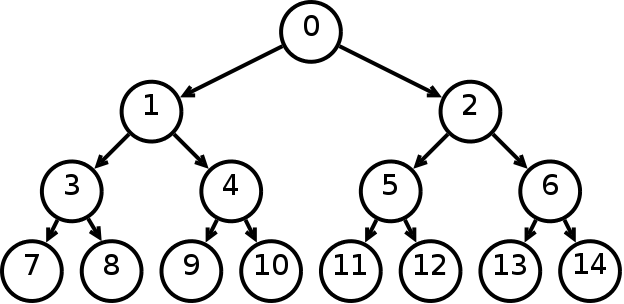
\includegraphics[width=4in]{images/heap.png}
\caption{Example of a heap data structure. The number represents not the data in the heap but the numbering of the nodes.}
\end{figure}

It starts from the top node, called the {\it root}. Each node has zero, one, or two children. It is called complete because nodes have been added from top to bottom and left to right, filling available slots. We can think of each level of the tree as a generation, where the older generation consists of one node, the next generation of two, the next of four, and so on. We can also number nodes from top to bottom and left to right, as in the image. This allows us to map the elements of a complete binary tree into the elements of an array.

We can implement a complete binary tree using a list, and the child--parent relations are given by the following formulas:
\begin{lstlisting}
proc heapParent(i: int): int = (i - 1) div 2
proc heapLeftChild(i: int): int = 2 * i + 1
proc heapRightChild(i: int): int = 2 * i + 2
\end{lstlisting}

We can store data (e.g., numbers) in the nodes (or in the corresponding array). If the data are
stored in such a way that the value at one node is always greater or equal than the value at its children, the array is called a {\it heap} and also a {\it priority queue}.

First of all, we need an algorithm to convert a list into a heap:

\begin{lstlisting}
proc heapifyOne*[T](a: var seq[T], i: int, heapsize = -1) =
  let heapsize = if heapsize < 0: a.len else: heapsize
  let left = 2 * i + 1
  let right = 2 * i + 2
  var largest = i
  if left < heapsize and a[left] > a[largest]:
    largest = left
  if right < heapsize and a[right] > a[largest]:
    largest = right
  if largest != i:
    swap(a[i], a[largest])
    heapifyOne(a, largest, heapsize)

proc heapify*[T](a: var seq[T]) =
  for i in countdown(a.len div 2 - 1, 0):
    heapifyOne(a, i)
\end{lstlisting}

Now we can call {\ft build\_heap} on any array or list and turn it into a heap.
Because the first element is by definition the smallest, we can use the heap to sort numbers in three steps:
\begin{itemize}
\item We turn the array into a heap
\item We extract the largest element
\item We apply recursion by sorting the remaining elements
\end{itemize}
Instead of using the preceding divide-and-conquer approach, it is better to use a dynamic programming approach. When we extract the largest element, we swap it with the last element of the array and make the heap one element shorter. The new, shorter heap does not need a full {\ft build\_heap} step because the only element out of order is the root node. We can fix this by a single call to {\ft heapify}.

This is a possible implementation for the {\ft heapsort}~\cite{heapsort}:

\begin{lstlisting}
proc heapsort*[T](a: var seq[T]) =
  heapify(a)
  for i in countdown(a.len - 1, 1):
    swap(a[0], a[i])
    heapifyOne(a, 0, i)
\end{lstlisting}

In the average and worst cases, it runs as fast as the quicksort, but in the best case, it is linear:

\begin{eqnarray}
T_{best} &\in &\Theta (n) \\
T_{average} &\in &\Theta (n\log n) \\
T_{worst} &\in &\Theta (n\log n) \\
T_{memory} &\in &\Theta (1)
\end{eqnarray}

\index{priority queue}

A heap can be used to implement a priority queue, for example, storage from which we can efficiently extract the largest element.

All we need is a function that allows extracting the root element from a heap (as we did in the {\ft heapsort} and {\ft heapify} of the remaining data) and a function to push a new value into the heap:

\begin{lstlisting}
proc heapPop*[T](a: var seq[T]): T =
  if a.len < 1:
    raise newException(IndexDefect, "Heap Underflow")
  result = a[0]
  a[0] = a[^1]
  a.setLen(a.len - 1)
  if a.len > 0:
    heapifyOne(a, 0)

proc heapPush*[T](a: var seq[T], value: T) =
  a.add value
  var i = a.len - 1
  while i > 0:
    let j = heapParent(i)
    if a[j] < a[i]:
      swap(a[i], a[j])
      i = j
    else:
      break
\end{lstlisting}

The running times for {\ft heap\_pop} and {\ft heap\_push} are the same:

\begin{eqnarray}
T_{best} &\in &\Theta (1) \\
T_{average} &\in &\Theta (\log n) \\
T_{worst} &\in &\Theta (\log n) \\
T_{memory} &\in &\Theta (1)
\end{eqnarray}

Here is an example:

\begin{lstlisting}
let a = @[6, 2, 7, 9, 3]
var heap: seq[int] = @[]
for element in a: heapPush(heap, element)
while heap.len > 0: echo heapPop(heap)
# 9
# 7
# 6
# 3
# 2
\end{lstlisting}

Heaps find application in many numerical algorithms. Nim's standard library provides {\ft std/heapqueue}, which offers similar functionality, except that {\ft HeapQueue} is a min-heap (pops the smallest element) while we defined a max-heap above:

\begin{lstlisting}
import std/heapqueue
let a = @[6, 2, 7, 9, 3]
var heap = initHeapQueue[int]()
for element in a: heap.push(element)
while heap.len > 0: echo heap.pop()
# 2
# 3
# 6
# 7
# 9
\end{lstlisting}

Notice that the order of {\ft pop} results is reversed because {\ft HeapQueue} is a min-heap.

\subsection{Binary search trees}

\index{binary tree}\index{binary search}

A binary tree is a tree in which each node has at most two children (left and right). A binary tree is called a {\it binary search tree} if the value of a node is always greater than or equal to the value of its left child and less than or equal to the value of its right child.

A binary search tree is a kind of storage that can efficiently be used for searching if a particular value is in the storage. In fact, if the value for which we are looking is less than the value of the root node, we only have to search the left branch of the tree, and if the value is greater, we only have to search the right branch. Using divide-and-conquer, searching each branch of the tree is even simpler than searching the entire tree because it is also a tree, but smaller.

This means that we can search simply by traversing the tree from top to bottom along some path down the tree. We choose the path by moving down and turning left or right at each node, until we find the element for which we are looking or we find the end of the tree. We can search $T(d)$, where $d$ is the depth of the tree. We will see later that it is possible to build binary trees where $d=\log n$.

To implement it, we need to have a class to represent a binary tree:

\begin{lstlisting}
type
  BinarySearchTree*[K, V] = ref object
    key*: K
    value*: V
    hasKey*: bool
    left*, right*: BinarySearchTree[K, V]

proc newBinarySearchTree*[K, V](): BinarySearchTree[K, V] =
  BinarySearchTree[K, V]()

proc `[]=`*[K, V](t: BinarySearchTree[K, V], key: K, value: V) =
  if not t.hasKey:
    t.key = key; t.value = value; t.hasKey = true
  elif key == t.key:
    t.value = value
  elif key < t.key:
    if t.left.isNil: t.left = newBinarySearchTree[K, V]()
    t.left[key] = value
  else:
    if t.right.isNil: t.right = newBinarySearchTree[K, V]()
    t.right[key] = value

proc `[]`*[K, V](t: BinarySearchTree[K, V], key: K): V =
  if not t.hasKey: return default(V)
  if key == t.key: return t.value
  elif key < t.key and not t.left.isNil: return t.left[key]
  elif key > t.key and not t.right.isNil: return t.right[key]
  else: return default(V)

proc min*[K, V](t: BinarySearchTree[K, V]): (K, V) =
  var node = t
  while not node.left.isNil:
    node = node.left
  (node.key, node.value)

proc max*[K, V](t: BinarySearchTree[K, V]): (K, V) =
  var node = t
  while not node.right.isNil:
    node = node.right
  (node.key, node.value)
\end{lstlisting}

The binary tree can be used as follows:

\begin{lstlisting}
let root = newBinarySearchTree[int, string]()
root[5] = "aaa"
root[3] = "bbb"
root[8] = "ccc"
echo root.left.key      # 3
echo root.left.value    # "bbb"
echo root[3]            # "bbb"
echo root.max()         # (8, "ccc")
\end{lstlisting}

Notice that an empty tree is treated as an exception, where {\ft key = None}.

\goodbreak\subsection{Other types of trees}

There are many other types of trees. \index{AVL tree}

For example, AVL trees are binary search trees that are rebalanced after each
insertion or deletion. They are rebalanced in such a way that for each node, the
height of the left subtree minus the height of the right subtree is more or less the same. The rebalance operation can be done in $O(\log n)$.

For an AVL tree, the time for inserting or removing an element is given by

\begin{eqnarray}
T_{best} &\in &\Theta (1) \\
T_{average} &\in &\Theta (\log n) \\
T_{worst} &\in &\Theta (\log n) \\
\end{eqnarray}

\index{k-tree}\index{B-tree}

Until now, we have considered binary trees (each node has two children and
stores one value). We can generalize this to $k$ trees, for which each node has $k$
children and stores more than one value.

B-trees are a type of k-tree optimized to read and write large blocks of data. They are normally used to implement database indices and are designed to minimize the amount of data to move when the tree is rebalanced.

\goodbreak\section{Graph algorithms}

\index{graphs}\index{links}\index{vertices}\index{walk}\index{path}\index{cycle}

A {\it graph} $G$ is a set of {\it vertices} $V$ and a set of {\it links} (also called {\it edges}) connecting those vertices $E$. Each link connects one vertex to another.

As an example, you can think of a set of cities connected by roads. The cities are the vertices and the roads are the links.

A link may have attributes. In the case of a road, it could be the name of the road or its length.

In general, a link, indicated with the notation $e_{ij}$, connecting vertex $%
i $ with vertex $j$ is called a {\it directed link}. If the link has no
direction $e_{ij}=e_{ji}$, it is called an undirected link. A graph that
contains only undirected links is an {\it undirected graph}; otherwise, it is
a {\it directed graph}.

In the road analogy, some roads can be ``one way'' (directed links) and some can be ``two way'' (undirected links).

A {\it walk} is an alternating sequence of vertices and links, with each
link being incident to the vertices immediately preceding and succeeding it
in the sequence. A {\it trail} is a walk with no repeated links.

A {\it path} is a walk with no repeated vertices. A walk is closed if the
initial vertex is also the terminal vertex.

A {\it cycle} is a closed trail with at least one edge and with no repeated
vertices, except that the initial vertex is also the terminal vertex.

A graph that contains no cycles is an {\it acyclic graph}. Any connected
acyclic undirected graph is also a {\it tree}.

\index{graph loop}

A {\it loop} is a one-link path connecting a vertex with itself.

\index{connected graph}

A non null graph is {\it connected} if, for every pair of vertices, there is
a walk whose ends are the given vertices. Let us write $i%
\symbol{126}j$ if there is a path from $i$ to $j$. Then $\symbol{126}$ is an
equivalence relation. The equivalence classes under $\symbol{126}$ are the
vertex sets of the connected components of $G$. A connected graph is therefore
a graph with exactly one connected component.

\index{complete graph}

A graph is called {\it complete} when every pair of vertices is connected by
a link (or edge).

\index{clique}

A {\it \ clique } of a graph is a subset of vertices in which every pair is an
edge.

\index{degree of a graph}

The {\it degree} of a vertex of a graph is the number of edges incident to
it.

If $i$ and $j$ are vertices, the {\it distance} from $i$ to $j$, written $%
d_{ij}$, is the minimum length of any path from $i$ to $j$. In a connected
undirected graph, the length of links induces a metric because for every two vertices, we can define their distance as the length of the shortest path connecting them.

The {\it eccentricity}, $e(i)$, of the vertex $i$ is the maximum value of $%
d_{ij}$, where $j$ is allowed to range over all of the vertices of the graph.  This gives the largest shortest distance to any connected node in the graph.

The {\it subgraph} of $G$ induced by a subset $W$ of its vertices $V$ ($%
W\subseteq V$) is the graph formed by the vertices in $W$ and all edges
whose two endpoints are in $W$.

The graph is the more complex of the data structures considered so far because it includes the tree as a particular case (yes, a tree is also a graph, but in general, a graph is not a tree), and the tree includes a list as a particular case (yes, a list is a tree in which every node has no more than one child); therefore a list is also a particular case of a graph.

The graph is such a general data structure that it can be used to model the brain. Think of neurons as vertices and synapses as links connecting them. We push this analogy later by implementing a simple neural network simulator.

In what follows, we represent a graph in the following way, where links are edges:

\begin{lstlisting}
let vertices = @["A", "B", "C", "D", "E"]
let links = @[(0, 1), (1, 2), (1, 3), (2, 5), (3, 4), (3, 2)]
let graph = (vertices, links)
\end{lstlisting}

Vertices are stored in a list or array and so are links. Each link is a tuple containing the ID of the source vertex, the ID of the target vertex, and perhaps optional parameters.  Optional parameters are discussed later, but for now, they may include link details such as length, speed, reliability, or billing rate.

\subsection{Breadth-first search}

\index{breadth-first search}

The breadth-first search~\cite{bfs} (BFS) is an algorithm designed to visit all vertices in a connected graph. In the cities analogy, we are looking for a travel strategy to make sure we visit every city reachable by roads, once and only once.

The algorithm begins at one vertex, the origin, and expands out, eventually visiting each node in the graph that is somehow connected to the origin vertex. Its main feature is that it explores the neighbors of the current vertex before moving on to explore remote vertices and their neighbors. It visits other vertices in the same order in which they are discovered.

The algorithm starts by building a table of neighbors so that for each vertex, it knows which other vertices it is connected to. It then maintains two lists, a list of blacknodes (defined as vertices that have been visited) and graynodes (defined as vertices that have been discovered because the algorithm has visited its neighbor). It returns a list of blacknodes in the order in which they have been visited.

Here is the algorithm:

%%% META:FILE:nlib/graph.nim
\begin{lstlisting}[caption={in file: {\ft nlib/graph.nim}}]
proc breadthFirstSearch*[V](
    graph: tuple[vertices: seq[V], links: seq[(int, int)]],
    start: int): seq[int] =
  var blacknodes: seq[int] = @[]
  var graynodes = @[start]
  var neighbors = newSeq[seq[int]](graph.vertices.len)
  for link in graph.links:
    neighbors[link[0]].add link[1]
  while graynodes.len > 0:
    let current = graynodes.pop()
    for neighbor in neighbors[current]:
      if neighbor notin blacknodes and neighbor notin graynodes:
        graynodes.insert(neighbor, 0)
    blacknodes.add current
  result = blacknodes
\end{lstlisting}

The BFS algorithm scales as follows:
\begin{eqnarray}
T_{best} &\in &\Theta (n_E+n_V) \\
T_{average} &\in &\Theta (n_E+n_V) \\
T_{worst} &\in &\Theta (n_E+n_V) \\
T_{memory} &\in &\Theta (n)
\end{eqnarray}

\subsection{Depth-first search}

\index{depth-first search}

The depth-first search~\cite{dfs} (DFS) algorithm is very similar to the BFS, but it takes the opposite approach and explores as far as possible along each branch before backtracking.

In the cities analogy, if the BFS was exploring cities in the neighborhood before moving farther away, the DFS does the opposite and brings us first to distant places before visiting other nearby cities.

Here is a possible implementation:

%%% META:FILE:nlib/graph.nim
\begin{lstlisting}[caption={in file: {\ft nlib/graph.nim}}]
proc depthFirstSearch*[V](
    graph: tuple[vertices: seq[V], links: seq[(int, int)]],
    start: int): seq[int] =
  var blacknodes: seq[int] = @[]
  var graynodes = @[start]
  var neighbors = newSeq[seq[int]](graph.vertices.len)
  for link in graph.links:
    neighbors[link[0]].add link[1]
  while graynodes.len > 0:
    let current = graynodes.pop()
    for neighbor in neighbors[current]:
      if neighbor notin blacknodes and neighbor notin graynodes:
        graynodes.add neighbor
    blacknodes.add current
  result = blacknodes
\end{lstlisting}

Notice that the BFS and the DFS differ by a single line, which determines whether graynodes is a queue (BSF) or a stack (DFS). When graynodes is a queue, the first vertex discovered is the first visited. When it is a stack, the last vertex discovered is the first visited.

The DFS algorithm goes as follows:
\begin{eqnarray}
T_{best} &\in &\Theta (n_E+n_V) \\
T_{average} &\in &\Theta (n_E+n_V) \\
T_{worst} &\in &\Theta (n_E+n_V) \\
T_{memory} &\in &\Theta (1)
\end{eqnarray}

\subsection{Disjoint sets}

\index{disjoint sets}

This is a data structure that can be used to store a set of sets and implements efficiently the join operation between sets.
Each element of a set is identified by a representative element. The algorithm starts by placing each element in a set of its own, so there are $n$ initial disjoint sets. Each is represented by itself. When two sets are joined, the representative element of the latter is made to point to the representative element of the former. The set of sets is stored as an array of integers. If at position $i$ the array stores a negative number, this number is interpreted as being the representative element of its own set. If the number stored at position $i$ is instead a nonnegative number $j$, it means that it belongs to a set that was joined with the set containing $j$.

Here is the implementation:

\index{class!DisjointSets}

%%% META:FILE:nlib/graph.nim
\begin{lstlisting}[caption={in file: {\ft nlib/graph.nim}}]
type
  DisjointSets* = ref object
    sets*: seq[int]
    counter*: int

proc newDisjointSets*(n: int): DisjointSets =
  result = DisjointSets(sets: newSeq[int](n), counter: n)
  for i in 0 ..< n: result.sets[i] = -1

proc parent*(d: DisjointSets, i: int): int =
  var i = i
  while true:
    let j = d.sets[i]
    if j < 0: return i
    i = j

proc join*(d: DisjointSets, i, j: int): bool =
  let pi = d.parent(i)
  let pj = d.parent(j)
  if pi != pj:
    d.sets[pi] += d.sets[pj]
    d.sets[pj] = pi
    dec d.counter
    return true   # they have been joined
  return false    # they were already joined

proc joined*(d: DisjointSets, i, j: int): bool =
  d.parent(i) == d.parent(j)

proc len*(d: DisjointSets): int = d.counter
\end{lstlisting}

Notice that we added a member variable counter that is initialized to the number of disjoint sets and is decreased by one every time two sets are merged. This allows us to keep track of how many disjoint sets exist at each time. We also override the {\ft \_\_len\_\_} operator so that we can check the value of the counter using the {\ft len} function on a {\ft DisjointSet}.

As an example of application, here is a code that builds a $n^d$ maze. It may be easier to picture it with $d=2$, a two-dimensional maze. The algorithm works by assuming there is a wall connecting any couple of two adjacent cells. It labels the cells using an integer index.
It puts all the cells into a {\ft DisjointSets} data structure and then keeps tearing down walls at random. Two cells on the maze belong to the same set if they are connected, for example, if there is a path that connects them. At the beginning, each cell is its own set because it is isolated by walls.
Walls are torn down by being removed from the list {\ft wall} if the wall was separating two disjoint sets of cells. Walls are torn down until all cells belong to the same set, for example, there is a path connecting any cell to any cell:

%%% META:FILE:nlib/graph.nim
\begin{lstlisting}[caption={in file: {\ft nlib/graph.nim}}]
proc makeMaze*(n, d: int): tuple[walls, tornDownWalls: seq[(int, int)]] =
  var walls: seq[(int, int)] = @[]
  let total = n ^ d
  for i in 0 ..< n * n:
    for j in 0 ..< d:
      if (i div (n ^ j)) mod n + 1 < n:
        walls.add (i, i + n ^ j)
  var tornDownWalls: seq[(int, int)] = @[]
  let ds = newDisjointSets(total)
  shuffle(walls)
  for wall in walls:
    if ds.join(wall[0], wall[1]):
      tornDownWalls.add wall
    if ds.len == 1:
      break
  var remaining: seq[(int, int)] = @[]
  for wall in walls:
    if wall notin tornDownWalls:
      remaining.add wall
  (remaining, tornDownWalls)
\end{lstlisting}

Here is an example of how to use it. This example also draws the walls and the border of the maze:

\begin{lstlisting}
let (walls, tornDownWalls) = makeMaze(n = 20, d = 2)
\end{lstlisting}

The following figure shows a representation of a generated maze:

\begin{figure}[ht]
\centering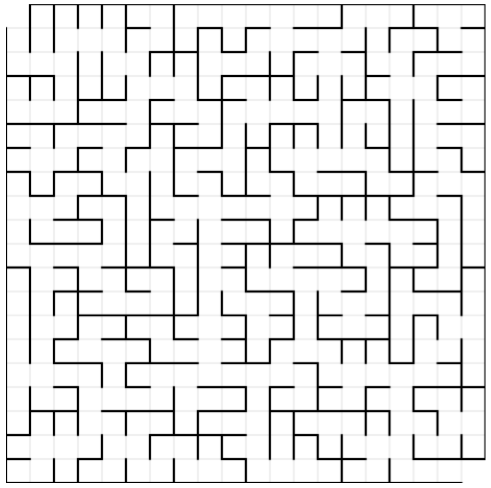
\includegraphics[width=2in]{images/maze1.png}
\caption{Example of a maze as generated using the {\ft DisjointSets} algorithm.}
\end{figure}

\subsection{Minimum spanning tree: Kruskal}

\index{minimum spanning tree}\index{Kruskal}

Given a connected graph with weighted links (links with a weight or length), a {\it minimum spanning tree} is a subset of that graph that connects all vertices of the original graph, and the sum of the link weights is minimal. This subgraph is also a tree because the condition of minimal weight implies that there is only one path connecting each couple of vertices.

\begin{figure}[ht]
\centering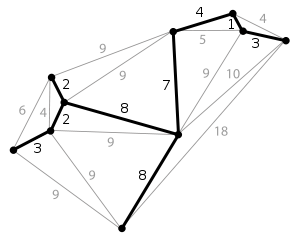
\includegraphics[width=2in]{images/mst.png}
\caption{Example of a minimum spanning tree subgraph of a larger graph. The numbers on the links indicate their weight or length.}
\end{figure}

One algorithm to build the minimal spanning tree of a graph is the Kruskal~\cite{kruskal} algorithm. It works by placing all vertices in a {\ft DisjointSets} structure and looping over links in order of their weight. If the link connects two vertices belonging to different sets, the link is selected to be part of the minimum spanning tree, and the two sets are joined, else the link is ignored. The Kruskal algorithm assumes an undirected graph, for example, all links are bidirectional, and the weight of a link is the same in both directions:

%%% META:FILE:nlib/graph.nim
\begin{lstlisting}[caption={in file: {\ft nlib/graph.nim}}]
import std/algorithm

proc kruskal*[V](
    graph: tuple[vertices: seq[V],
                 links: seq[(int, int, float)]]
    ): seq[(int, int, float)] =
  var links = graph.links
  links.sort(proc(a, b: (int, int, float)): int = cmp(a[2], b[2]))
  let s = newDisjointSets(graph.vertices.len)
  for link in links:
    let (source, dest, length) = link
    if s.join(source, dest):
      result.add (source, dest, length)
\end{lstlisting}

The Kruskal algorithm goes as follows:
\begin{eqnarray}
T_{worst} &\in &\Theta (n_E\log n_V) \\
T_{memory} &\in &\Theta (n_E)
\end{eqnarray}

We provide an example of application in the next subsection.

\goodbreak\subsection{Minimum spanning tree: Prim}

The Prim~\cite{prim} algorithm solves the same problem as the Kruskal algorithm, but the Prim algorithm works on a directed graph. It works by placing all vertices in a minimum priority queue where the queue metric for each vertex is the length, or weighted value, of a link connecting the vertex to the closest known neighbor vertex. At each iteration, the algorithm pops a vertex from the priority queue, loops over its neighbors (adjacent links), and, if it finds that one of its neighbors is already in the queue and it is possible to connect it to the current vertex using a shorter link than the one connecting the neighbor to its current closest vertex, the neighbor information is then updated. The algorithm loops until there are no vertices in the priority queue.

The Prim algorithm also differs from the Kruskal algorithm because the former needs a starting vertex, whereas the latter does not. The result when interpreted as a subgraph does not depend on the starting vertex:

%%% META:FILE:nlib/graph.nim
\begin{lstlisting}[caption={in file: {\ft nlib/graph.nim}}]
const PRIM_INFINITY* = 1e100

type
  PrimVertex* = ref object
    id*: int
    closest*: PrimVertex
    closestDist*: float
    neighbors*: seq[(int, float)]

proc newPrimVertex*(id: int, links: seq[(int, int, float)]): PrimVertex =
  result = PrimVertex(id: id, closest: nil, closestDist: PRIM_INFINITY)
  for link in links:
    if link[0] == id:
      result.neighbors.add (link[1], link[2])

proc `<`*(a, b: PrimVertex): bool = a.closestDist < b.closestDist

proc prim*[V](
    graph: tuple[vertices: seq[V], links: seq[(int, int, float)]],
    start: int): seq[(int, int, float)] =
  var p: seq[PrimVertex] = @[]
  for i in 0 ..< graph.vertices.len:
    p.add newPrimVertex(i, graph.links)
  var q: seq[PrimVertex] = @[]
  for i in 0 ..< graph.vertices.len:
    if i != start: q.add p[i]
  var vertex = p[start]
  while q.len > 0:
    for (neighborId, length) in vertex.neighbors:
      let neighbor = p[neighborId]
      if neighbor in q and length < neighbor.closestDist:
        neighbor.closest = vertex
        neighbor.closestDist = length
    q.sort(proc(a, b: PrimVertex): int = cmp(a.closestDist, b.closestDist))
    vertex = q[0]
    q.delete(0)
  for v in p:
    if v.id != start:
      result.add (v.id, v.closest.id, v.closestDist)
\end{lstlisting}

\begin{lstlisting}
let vertices = toSeq(0 ..< 10)
var links: seq[(int, int, float)] = @[]
for i in vertices:
  for j in vertices:
    links.add (i, j, abs(sin(float(i + j + 1))))
let graph = (vertices, links)
let mst = prim(graph, 0)
for link in mst: echo link
# (1, 4, 0.279...)
# (2, 0, 0.141...)
# (3, 2, 0.279...)
# (4, 1, 0.279...)
# (5, 0, 0.279...)
# (6, 2, 0.412...)
# (7, 8, 0.287...)
# (8, 7, 0.287...)
# (9, 6, 0.287...)
\end{lstlisting}

The Prim algorithm, when using a priority queue for $Q$, goes as follows:
\begin{eqnarray}
T_{worst} &\in &\Theta (n_E+n_V\log n_V) \\
T_{memory} &\in &\Theta (n_E)
\end{eqnarray}

One important application of the minimum spanning tree is in evolutionary biology. Consider, for example, the DNA for the genes that produce hemoglobin, a molecule responsible for the transport of oxygen in blood. This protein is present in every animal, and the gene is also present in the DNA of every known animal. Yet its DNA structure is a little different. One can select a pool of animals and, for each two of them, compute the similarity of the DNA of their hemoglobin genes using the {\ft lcs} algorithm discussed later. One can then link each two animals by a metric that represents how similar the two animals are. We can then run the Prim or the Kruskal algorithm to find the minimum spanning tree. The tree represents the most likely evolutionary tree connecting those animal species. Actually, three genes are responsible for hemoglobin ({\it HBA1}, {\it HBA2}, and {\it HBB}). By performing the analysis on different genes and comparing the results, it is possible to establish a consistency check of the results.~\cite{evolutionary}

Similar studies are performed routinely in evolutionary biology. They can also be applied to viruses to understand how viruses evolved over time.~\cite{korber}

\subsection{Single-source shortest paths: Dijkstra}

\index{single-source shortest paths}\index{Dijkstra}

The Dijkstra~\cite{dijkstra} algorithm solves a similar problem to the Kruskal and Prim algorithms. Given a graph, it computes, for each vertex, the shortest path connecting the vertex to a starting (or source, or root) vertex. The collection of links on all the paths defines the {\it single-source shortest paths}.

It works, like Prim, by placing all vertices in a min priority queue where the queue metric for each vertex is the length of the path connecting the vertex to the source. At each iteration, the algorithm pops a vertex from the priority queue, loops over its neighbors (adjacent links), and, if it finds that one of its neighbors is already in the queue and it is possible to connect it to the current vertex using a link that makes the path to the source shorter, the neighbor information is updated. The algorithm loops until there are no more vertices in the priority queue.

The implementation of this algorithm is almost identical to the Prim algorithm, except for two lines:

%%% META:FILE:nlib/graph.nim
\begin{lstlisting}[caption={in file: {\ft nlib/graph.nim}}]
proc dijkstra*[V](
    graph: tuple[vertices: seq[V], links: seq[(int, int, float)]],
    start: int): seq[(int, int, float)] =
  var p: seq[PrimVertex] = @[]
  for i in 0 ..< graph.vertices.len:
    p.add newPrimVertex(i, graph.links)
  var q: seq[PrimVertex] = @[]
  for i in 0 ..< graph.vertices.len:
    if i != start: q.add p[i]
  var vertex = p[start]
  vertex.closestDist = 0
  while q.len > 0:
    for (neighborId, length) in vertex.neighbors:
      let neighbor = p[neighborId]
      let dist = length + vertex.closestDist
      if neighbor in q and dist < neighbor.closestDist:
        neighbor.closest = vertex
        neighbor.closestDist = dist
    q.sort(proc(a, b: PrimVertex): int = cmp(a.closestDist, b.closestDist))
    vertex = q[0]
    q.delete(0)
  for v in p:
    if v.id != start:
      result.add (v.id, v.closest.id, v.closestDist)
\end{lstlisting}

\begin{lstlisting}
let vertices = toSeq(0 ..< 10)
var links: seq[(int, int, float)] = @[]
for i in vertices:
  for j in vertices:
    links.add (i, j, abs(sin(float(i + j + 1))))
let graph = (vertices, links)
let paths = dijkstra(graph, 0)
for link in paths: echo link
# (1, 2, 0.897...)
# (2, 0, 0.141...)
# (3, 2, 0.420...)
# (4, 2, 0.798...)
# (5, 0, 0.279...)
# (6, 2, 0.553...)
# (7, 2, 0.685...)
# (8, 0, 0.412...)
# (9, 0, 0.544...)
\end{lstlisting}

The Dijkstra algorithm goes as follows:
\begin{eqnarray}
T_{worst} &\in &\Theta (n_E+n_V\log n_V) \\
T_{memory} &\in &\Theta (n_E)
\end{eqnarray}

An application of the Dijkstra is in solving a maze such as the one built when discussing disjoint sets. To use the Dijkstra algorithm, we need to generate a maze, take the links representing torn-down walls, and use them to build an undirected graph. This is done by symmetrizing the links (if $i$ and $j$ are connected, $j$ and $i$ are also connected) and adding to each link a length (1, because all links connect next-neighbor cells):


\begin{lstlisting}
let (n, d) = (4, 2)
let (mazeWalls, tornDown) = makeMaze(n, d)
var symmetrizedLinks: seq[(int, int, float)] = @[]
for (i, j) in tornDown: symmetrizedLinks.add (i, j, 1.0)
for (i, j) in tornDown: symmetrizedLinks.add (j, i, 1.0)
let graph = (toSeq(0 ..< n * n), symmetrizedLinks)
let mst = dijkstra(graph, 0)
var paths = initTable[int, (int, float)]()
for (i, j, dd) in mst: paths[i] = (j, dd)
\end{lstlisting}

Given a maze cell {\ft i}, {\ft path[i]} gives us a tuple $(j, d)$ where $d$ is the number of steps for the shortest path to reach the origin (0) and $j$ is the ID of the next cell along this path.
The following figure shows a generated maze and a reconstructed path connecting an arbitrary cell to the origin:

\begin{figure}[ht]
\centering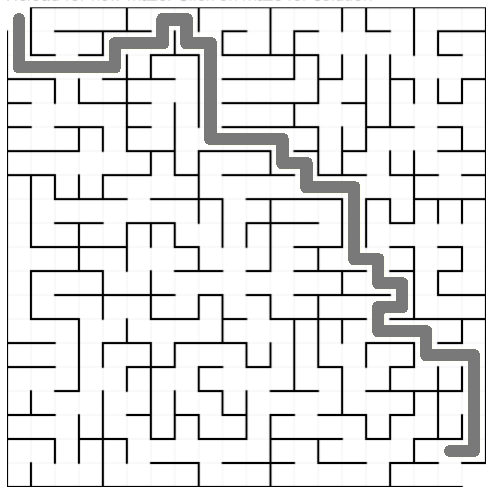
\includegraphics[width=2in]{images/maze2.png}
\caption{The result shows an application of the Dijkstra algorithm for the single source shortest path applied to solve a maze.}
\end{figure}

\goodbreak\section{Greedy algorithms}

\subsection{Huffman encoding}

\index{greedy algorithms}
\index{Huffman encoding}\index{Shannon-Fano}

The {\it Shannon--Fano encoding}~\cite{shannon}\cite{fano} (also known as {\bf minimal prefix code}) is a lossless data compression algorithm.
In this encoding, each character in a string is mapped into a sequence of bits
so characters that appear with less frequency are encoded with a longer
sequence of bits, whereas characters that appear with more frequency are
encoded with a shorter sequence.

The {\it Huffman encoding}~\cite{huffman} is an implementation of the Shannon--Fano encoding, but the sequence of bits into which each character is mapped is chosen such that the length of the compressed string is minimal.
This choice is constructed in the following way.
We associate a tree with each character
in the string to compress. Each tree is a trivial tree containing only one
node: the root node. We then associate with the root node the frequency of the
character representing the tree. We then extract from the list of trees the
two trees with rarest or lowest frequency: t1 and t2. We form a new tree, t3, we attach
t1 and t2 to t3, and we associate a frequency with t3 equal to the sum of the
frequencies of t1 and t2. We repeat this operation until the list of trees
contains only one tree. At this point, we associate a sequence of bits with
each node of the tree. Each bit corresponds to one level on the tree. The
more frequent characters end up being closer to the root and are encoded
with a few bits, while rare characters are far from the root and encoded with
more bits.

PKZIP, ARJ, ARC, JPEG, MPEG3 (mp3), MPEG4, and other
compressed file formats all use the Huffman coding algorithm for compressing
strings. Note that Huffman is a compression algorithm with
no information loss. In the JPEG and MPEG compression algorithms, Huffman algorithms are
combined with some form or cut of the Fourier spectrum (e.g., MP3 is
an audio compression format in which frequencies below 2 KHz are dumped and not
compressed because they are not audible). Therefore the JPEG and MPEG
formats are referred to as compression with information loss.

Here is a possible implementation of Huffman encoding using the {\ft std/heapqueue} module. For the priority-queue ordering to be correct we wrap each tree (the set of symbols it represents and their cumulative frequency) into a {\ft HuffmanNode} record and overload the {\ft <} operator on it.

%%% META:FILE:nlib/compression.nim
\begin{lstlisting}[caption={in file: {\ft nlib/compression.nim}}]
import std/heapqueue

type
  HuffmanTreeKind* = enum hkLeaf, hkNode
  HuffmanTree* = ref object
    frequency*: int
    case kind*: HuffmanTreeKind
    of hkLeaf: symbol*: char
    of hkNode: left*, right*: HuffmanTree

  HuffmanNode* = object
    frequency*: int
    tree*: HuffmanTree

proc `<`*(a, b: HuffmanNode): bool = a.frequency < b.frequency

proc inorderTreeWalk(t: HuffmanTree, key: string,
                     keys: var Table[char, string]) =
  case t.kind
  of hkLeaf: keys[t.symbol] = key
  of hkNode:
    inorderTreeWalk(t.left, key & "0", keys)
    inorderTreeWalk(t.right, key & "1", keys)

proc encodeHuffman*(input: string): (Table[char, string], string) =
  var symbols = initTable[char, int]()
  for s in input:
    symbols[s] = symbols.getOrDefault(s, 0) + 1
  var heap = initHeapQueue[HuffmanNode]()
  for k, f in symbols:
    heap.push(HuffmanNode(frequency: f,
              tree: HuffmanTree(kind: hkLeaf, frequency: f, symbol: k)))
  while heap.len > 1:
    let n1 = heap.pop()
    let n2 = heap.pop()
    let merged = HuffmanTree(kind: hkNode,
                             frequency: n1.frequency + n2.frequency,
                             left: n1.tree, right: n2.tree)
    heap.push(HuffmanNode(frequency: merged.frequency, tree: merged))
  var symbolMap = initTable[char, string]()
  inorderTreeWalk(heap[0].tree, "", symbolMap)
  var encoded = ""
  for s in input: encoded.add symbolMap[s]
  (symbolMap, encoded)

proc decodeHuffman*(keys: Table[char, string], encoded: string): string =
  var reversed = initTable[string, char]()
  for k, v in keys: reversed[v] = k
  var i = 0
  for j in 1 .. encoded.len:
    let chunk = encoded[i ..< j]
    if chunk in reversed:
      result.add reversed[chunk]
      i = j
\end{lstlisting}

We can use it as follows:

\begin{lstlisting}
let input = "this is a nice day"
let (keys, encoded) = encodeHuffman(input)
echo encoded
# 00100101110011101100111011111000111100001111010000011110100
let decoded = decodeHuffman(keys, encoded)
echo decoded == input            # true
echo 1.0 * float(input.len) / (float(encoded.len) / 8.0)
# 2.44...
\end{lstlisting}

We managed to compress the original data by a factor 2.57.

\index{entropy}

We can ask how good is this compression factor.
The maximum theoretical best compression factor is given by the Shannon {\it entropy}, defined as

\begin{equation}
E = -\sum_u w_i \log_2 w_i
\end{equation}
where $w_i$ is the relative frequency of each symbol.
In our case, this is easy to compute as

\begin{lstlisting}
import std/[math, sets]
let input = "this is a nice day"
var alphabet: HashSet[char]
for c in input: alphabet.incl c
var w: seq[float] = @[]
for c in alphabet:
  w.add float(input.count(c)) / float(input.len)
var entropy = 0.0
for wi in w: entropy -= wi * log2(wi)
echo entropy   # 3.23...
\end{lstlisting}

How could we have done better? Notice for example that the Huffman encoding does not take into account the order in which symbols appear. The original string contains the triple ``is'' twice, and we could have taken advantage of that pattern, but we did not.

Our choice of using characters as symbols is arbitrary. We could have used a couple of characters as symbols or triplets or any other subsequences of bytes of the original input. We could also have used symbols of different lengths for different parts of the input (we could have used a single symbol for ``is''). A different choice would have given a different compression ratio, perhaps better, perhaps worse.

\subsection{Longest common subsequence}

\index{longest common subsequence}\index{DNA}

Given two sequences of characters $S_1$ and $S_2$, this is the problem of determining the length of the longest common subsequence (LCS) that is a subsequence of both $S_1$ and $S_2$.

There are several applications for the LCS~\cite{bergroth} algorithm:

\begin{itemize}
\item  {\bf Molecular biology}: DNA sequences (genes) can be represented as sequences of four letters ACGT, corresponding to the four sub-molecules forming DNA. When biologists find a new sequence, they want to find similar sequences or ones that are close. One way of computing how similar two sequences are is to find the length of their LCS.

\item  {\bf File comparison}: The Unix program {\ft diff} is used to compare
two different versions of the same file, to determine what changes have been
made to the file. It works by finding a LCS of the
lines of the two files and displays the set of lines that have changed. In
this instance of the problem, we should think of each line of a file as being
a single complicated character.

\item  {\bf Spelling correction}: If some text contains a word, w, that is not
in the dictionary, a ``close'' word (e.g., one with a small edit distance to w)
may be suggested as a correction. Transposition errors are common in written
text. A transposition can be treated as a deletion plus an insertion, but a
simple variation on the algorithm can treat a transposition as a single
point mutation.

\item  {\bf Speech recognition}: Algorithms similar to the LCS are used in
some speech recognition systems---find a close match between a new utterance
and one in a library of classified utterances.
\end{itemize}

Let"s start with some simple observations about the LCS problem. If we have
two strings, say, ``ATGGCACTACGAT'' and ``ATCGAGC, '' we can represent a
subsequence as a way of writing the two so that certain letters line up:
\begin{lstlisting}
     ATGGCACTACGAT
     || | |   |
     ATCG AG  C
\end{lstlisting}

From this we can observe the following simple fact: if the two strings start
with the same letter, it"s always safe to choose that starting letter as the
first character of the subsequence. This is because, if you have some other
subsequence, represented as a collection of lines as drawn here, you can
``push'' the leftmost line to the start of the two strings without causing
any other crossings and get a representation of an equally long subsequence
that does start this way.

Conversely, suppose that, like in the preceding example, the two first
characters differ. Then it is not possible for both of them to be part of a
common subsequence.  There are three possible choices: remove the first letter from
either one of the strings or remove the letter from both strings.

Finally, observe that once we"ve decided what to do with the first
characters of the strings, the remaining subproblem is again a LCS problem on two shorter strings. Therefore we can solve
it recursively. However, because we don"t know which choice of the three to take, 
we will take them all and see which choice returns the best result.

Rather than finding the subsequence itself, it turns out to be more
efficient to find the length of the longest subsequence. Then, in
the case where the first characters differ, we can determine which
subproblem gives the correct solution by solving both and taking the max of
the resulting subsequence lengths. Once we turn this into a dynamic
programming algorithm, we get the following:

%%% META:FILE:nlib/text.nim
\begin{lstlisting}[caption={in file: {\ft nlib/text.nim}}]
proc lcs*(a, b: string): int =
  var previous = newSeq[int](b.len)
  var current = newSeq[int](b.len)
  for i, r in a:
    for j, c in b:
      var e: int
      if r == c:
        e = (if i * j > 0: previous[j-1] + 1 else: 1)
      else:
        let up = if i > 0: previous[j] else: 0
        let lf = if j > 0: current[j-1] else: 0
        e = max(up, lf)
      current[j] = e
    previous = current
  result = current[^1]
\end{lstlisting}

Here is an example:

\begin{lstlisting}
let dna1 = "ATGCTTTAGAGGATGCGTAGATAGCTAAATAGCTCGCTAGA"
let dna2 = "GATAGGTACCACAATAATAAGGATAGCTCGCAAATCCTCGA"
echo lcs(dna1, dna2)   # 26
\end{lstlisting}

The algorithms can be shown to be $O(nm)$ (where $m=$ len(a) and $n=$ len(b)).

Another application of this algorithm is in the Unix {\ft diff} utility. Here is a simple example to find the number of common lines between two files:

\begin{lstlisting}
let a = readFile("file1.txt")
let b = readFile("file2.txt")
echo lcs(a, b)
\end{lstlisting}

\subsection{Needleman--Wunsch}

\index{Needleman--Wunsch}\index{global alignment}

With some minor changes to the LCS algorithm, we obtain the Needleman--Wunsch algorithm~\cite{needleman}, which solves the problem of {\it global sequence alignment}. The changes are that, instead of using only two alternating rows ({\ft c} and {\ft d} for storing the temporary results, we store all temporary results in an array {\ft z}; when two matching symbols are found and they are not consecutive, we apply a penalty equal to $p^m$, where $m$ is the distance between the two matches and is also the size of the gap in the matching subsequence:


%%% META:FILE:nlib/text.nim
\begin{lstlisting}[caption={in file: {\ft nlib/text.nim}}]
proc needlemanWunsch*(a, b: string, p = 0.97): seq[seq[float]] =
  var z: seq[seq[float]] = @[]
  for i, r in a:
    var row: seq[float] = @[]
    for j, c in b:
      var e: float
      if r == c:
        e = if i * j > 0: z[i-1][j-1] + 1.0 else: 1.0
      else:
        let up = if i > 0: z[i-1][j] else: 0.0
        let lf = if j > 0: row[j-1] else: 0.0
        e = p * max(up, lf)
      row.add e
    z.add row
  result = z
\end{lstlisting}

This algorithm can be used to identify common subsequences of DNA between chromosomes (or in general common similar subsequences between any two strings of binary data). Here is an example in which we look for common genes in two randomly generated chromosomes:

\begin{lstlisting}
let bases = "ATGC"
randomize()
proc randString(n: int): string =
  for _ in 0 ..< n: result.add bases[rand(bases.len - 1)]
var genes: seq[string] = @[]
for _ in 0 ..< 20: genes.add randString(10)
var chromosome1, chromosome2 = ""
for _ in 0 ..< 10:
  chromosome1.add genes[rand(genes.len - 1)]
  chromosome2.add genes[rand(genes.len - 1)]
let z = needlemanWunsch(chromosome1, chromosome2)
# `z` is a 2D scoring matrix; the helper `saveHeatmap` (defined
# alongside `savePlot` in nlib.nim) renders it to an image file.
\end{lstlisting}

The output of the algorithm is the following image:

\begin{figure}[ht]
\centering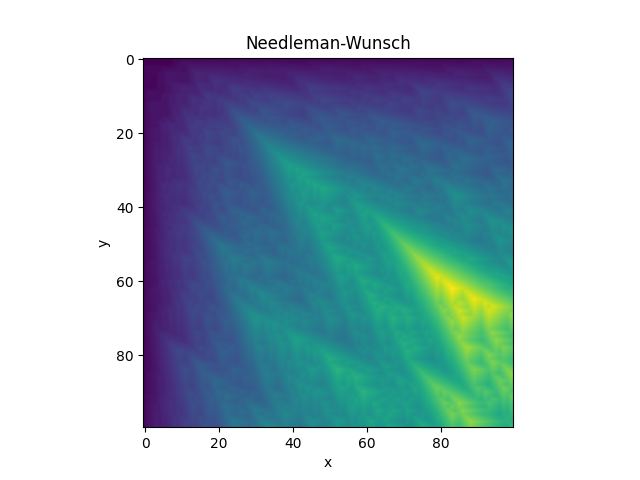
\includegraphics[width=4in]{images/needleman.png}
\caption{A Needleman and Wunsch plot sequence alignment. The arrow-like patterns indicate the point in the two sequences (represented by the $X$- and $Y$-coordinates) where the two sequences are more likely to align.}
\end{figure}

The arrow-like patterns in the figure correspond to locations where {\ft chromosome1} (Y coordinate) and where {\ft chromosome2} (X coordinate) have DNA in common. Those are the places where the sequences are more likely to be aligned for a more detailed comparison.

Optimized implementations of LCS and Needleman--Wunsch exist in many bioinformatics toolkits; in Nim, specialized packages wrap battle-tested C alignment tools through the foreign-function interface and expose comparable APIs.

\subsection{Continuous Knapsack}
\index{continuous knapsack}

Assume you want to fill your knapsack such that you will maximize the value of its contents~\cite{knapsack}.  However, you are limited by the volume your knapsack can hold. In the continuous knapsack, the amount of each product can vary continuously. In the discrete one, each product has a finite size, and you either carry it or no.

The continuous knapsack problem can be formulated as the problem of
maximizing
\begin{equation}
f(x)=a_0x_0+a_1x_1+...+a_nx_n
\end{equation}
given the constraint
\begin{equation}
b_0x_0+b_1x_1+...+b_nx_n\leq c
\end{equation}
where coefficients $a_i$, $b_i$, and $c$ are provided and $x_i\in [0, 1]$ are
to be determined.

Using financial terms, we can say that

\begin{itemize}
\item  The set $\{x_0, x_1, ..., x_n\}$ forms a portfolio

\item  $b_i$ is the cost of investment $i$

\item  $c$ is the total investment capital available

\item  $a_i$ is the expected return of investment for investment $i$

\item  $f(x)$ is the expected value of our portfolio $\{x_0, x_1, ..., x_n\}$
\end{itemize}

Here is the solving algorithm:

%%% META:FILE:nlib/finance.nim
\begin{lstlisting}[caption={in file: {\ft nlib/finance.nim}}]
proc continuumKnapsack*(a, b: seq[float], c: float):
                       (float, seq[(int, float)]) =
  var table: seq[(float, int)] = @[]
  for i in 0 ..< a.len: table.add (a[i] / b[i], i)
  table.sort(SortOrder.Descending)
  var f = 0.0
  var x: seq[(int, float)] = @[]
  var c = c
  for (y, i) in table:
    let quantity = min(c / b[i], 1.0)
    x.add (i, quantity)
    c -= b[i] * quantity
    f += a[i] * quantity
  (f, x)
\end{lstlisting}

This algorithm is dominated by the sort; therefore
\begin{equation}
T_{worst}(x)\in O(n\log n)
\end{equation}

\subsection{Discrete Knapsack}
\index{discrete knapsack}

The discrete Knapsack problem is very similar to the continuous knapsack
problem but $x_i\in \{0, 1\}$ (can only be 0 or 1).

Consider the jars of liquids replaced with baskets of objects, say, a basket each of gold bars, silver coins, copper beads, and Rolex watches.  How many of each item do you take?  The discrete knapsack problem does not consider ``baskets of items'' but rather all the items together.  In this example, dump out all the baskets and you have individual objects to take.  Which objects do you take, and which do you leave behind?

In this case, a greedy approach does not apply and the problem is, in general, 
NP complete. This concept is defined formally later but it means that there is no known algorithm that can solve this problem and that its order of growth is a polynomial. The best known algorithm has an exponential running time.

This kind of problem is unsolvable for large input.

If we assume that $c$ and $b_i$ are all multiples of a finite factor $\varepsilon$, then it is possible to solve the problem in $O(c/\varepsilon )$.
Even when there is not a finite factor $\varepsilon$, 
we can always round $c$ and $b_i$ to some finite precision $\varepsilon$, 
and we can conclude that, for any finite precision $\varepsilon$, we can
solve the problem in linear time. The algorithm that solves this problem
follows a dynamic programming approach.

We can reformulate the problem in terms of a simple capital budgeting
problem. We have to invest \$5M. We assume $\varepsilon =$\$1M. We are in
contact with three investment firms. Each offers a number of investment
opportunities characterized by an investment cost $c[i, j]$ and an expected
return of investment $r[i, j]$. The index $i$ labels the investment firm and
the index $j$ labels the different investment opportunities offered by the
firm. We have to build a portfolio that maximizes the return of investment.
We cannot select more than one investment for each firm, and we cannot select
fractions of investments.

Without loss of generality, we will assume that
\begin{equation}
c[i, j]\leq c[i, j+1]\text{ and }r[i, j]\leq r[i, j+1]
\end{equation}
which means that investment opportunities for each firm are sorted according
to their cost.

\medskip Consider the following explicit case:
\begin{equation}
\begin{tabular}{|l|l|l|l|l|l|l|}
\hline
& Firm & $i=0$ & Firm & $i=1$ & Firm & $i=2$ \\ \hline
proposal & $c[0, j]$ & $r[0, j]$ & $c[1, j]$ & $r[1, j]$ & $c[2, j]$ & $r[2, j]$
\\ \hline
$j=0$ & 0 & 0 & 0 & 0 & 0 & 0 \\ \hline
$j=1$ & 1 & 5 & 2 & 8 & 1 & 4 \\ \hline
$j=2$ & 2 & 6 & 3 & 9 & - & - \\ \hline
$j=3$ & - & - & 4 & 12 & - & - \\ \hline
\end{tabular}
\tag{Table 1}
\end{equation}
(table values are always multiples of $\varepsilon =$\$1M).

Notice that we can label each possible portfolio by a triplet $%
\{j_0, j_1, j_2\}$.

A straightforward way to solve this is to try all possibilities and choose
the best. In this case, there are only $3\times 4\times 2=24$ possible
portfolios. Many of these are infeasible (e.g., portfolio $\{2, 3, 0\}$
costs \$6M and we cannot afford it). Other portfolios are feasible but very
poor (like portfolio $\{0, 0, 1\}$, which is feasible but returns only \$4M).

Here are some disadvantages of total enumeration:

\begin{itemize}
\item  For larger problems, the enumeration of all possible solutions may not
be computationally feasible.

\item  Infeasible combinations may not be detectable a priori, leading to
inefficiency.

\item  Information about previously investigated combinations is not used to
eliminate inferior or infeasible combinations (unless we use memoization, 
but in this case the algorithm would grow polynomially in memory space).
\end{itemize}

We can, instead, use a dynamic programming approach.

We break the problem into three stages, and at each stage, we fill a table of
optimal investments for each discrete amount of money. At each stage $i$, we
only consider investments from firm $i$ and the table during the previous
stage.

So stage $0$ represents the money allocated to firm $0$, stage $1$ the money
to firm $1$, and stage $2$ the money to firm $2$.

STAGE\ ZERO: we maximize the return of investment considering only offers
from firm 0. We fill a table $f[0, k]$ with the maximum return of investment
if we invest $k$ million dollars in firm $0$:
\begin{equation}
f[0, k]=\max_{j|c[0, j]<k}r[0, j]  \label{stage0}
\end{equation}
\begin{equation*}
\begin{tabular}{|l|l|}
\hline
$k$ & $f[0, k]$ \\ \hline
0 & 0 \\ \hline
1 & 5 \\ \hline
2$^{ * }$ & 6$^{ * }$ \\ \hline
3 & 6 \\ \hline
4 & 6 \\ \hline
5 & 6 \\ \hline
\end{tabular}
\label{table0}
\end{equation*}

STAGE TWO: we maximize the return of investment considering offers from firm $%
1$ and the prior table. We fill a table $f[1, k]$ with the maximum return of
investment if we invest $k$ million dollars in firm $0$ and firm $1$:
\begin{equation}
f[1, k]=\max_{j|c[1, j]<k}r[1, j]+f[0, k-c[0, j]]  \label{stage1}
\end{equation}
\begin{equation*}
\begin{tabular}{|l|l|l|l|}
\hline
$k$ & $c[2, j]$ & $f[0, k-c[0, j]]$ & $f[1, k]$ \\ \hline
0 & 0 & 0 & 0 \\ \hline
1 & 0 & 1 & 5 \\ \hline
2 & 2 & 0 & 8 \\ \hline
3 & 2 & 1 & 9 \\ \hline
4 & 3 & 1 & 13 \\ \hline
5$^{ * }$ & 4$^{ * }$ & 1$^{ * }$ & 18$^{ * }$ \\ \hline
\end{tabular}
\label{table_stage2}
\end{equation*}

STAGE THREE: we maximize the return of investment considering offers from
firm $2$ and the preceding table. We fill a table $f[2, k]$ with the maximum
return of investment if we invest $k$ million dollars in firm $0$, firm $1$, 
and firm $2$:
\begin{equation}
f[2, k]=\max_{j|c[2, j]<k}r[2, j]+f[1, k-c[1, j]]  \label{stage2}
\end{equation}
\begin{equation*}
\begin{tabular}{|l|l|l|l|}
\hline
$k$ & $c[2, j]$ & $f[1, k-c[1, j]]$ & $f[2, k]$ \\ \hline
0 & 0 & 0 & 0 \\ \hline
1 & 0 & 1 & 5 \\ \hline
2 & 2 & 0 & 8 \\ \hline
3 & 2 & 1 & 9 \\ \hline
4 & 1 & 3 & 13 \\ \hline
5$^{ * }$ & 2$^{ * }$ & 3$^{ * }$ & 18$^{ * }$ \\ \hline
\end{tabular}
\label{table_stage3}
\end{equation*}
The maximum return of investment with \$5M is therefore \$18M. It can be
achieved by investing \$2M in firm 2 and \$3M in firms 0 and 1. The optimal
choice is marked with a star in each table. Note that to determine
how much money has to be allocated to maximize the return of
investment requires storing past tables to be able to look up the
solution to subproblems.

We can generalize eq.(\ref{stage1}) and eq.(\ref{stage2}) for any number of
investment firms (decision stages):

\begin{equation}
f[i, k]=\max_{j|c[i, j]<k}r[i, j]+f[i-1, k-c[i-1, j]]
\end{equation}

\goodbreak\section{Artificial intelligence and machine learning}

\index{artificial intelligence}\index{machine learning}

\goodbreak\subsection{Clustering algorithms}

\index{clustering}\index{hierarchical clustering}\index{k-means}

There are many algorithms available to cluster data~\cite{clustering}. They are all based on empirical principles because the clusters themselves are defined by the algorithm used to identify them. Normally we distinguish three categories:
\begin{itemize}
\item {\it Hierarchical clustering}: These algorithms start by considering each point a cluster of its own. At each iteration, the two clusters closest to each other are joined together, forming a larger cluster. Hierarchical clustering algorithms differ from each other about the rule used to determine the distance between clusters. The algorithm returns a tree representing the clusters that are joined, called a {\it dendrogram}.
\item {\it Centroid-based clustering}: These algorithms require that each point be represented by a vector and each cluster also be represented by a vector (centroid of the cluster). With each iteration, a better estimation for the centroids is given. An example of centroid-based clustering is {\it k-means} clustering. These algorithms require an a priori knowledge of the number of clusters and return the position of the centroids as well the set of points belonging to each cluster.
\item {\it Distribution-based clustering}: These algorithms are based on statistics (more than the other two categories). They assume the points are generated from a distribution (which must be known a priori) and determine the parameters of the distribution. It provides clustering because the distribution may be a sum of more than one localized distribution (each being a cluster).
\end{itemize}

Both {\it k}-means and distribution-based clustering assume an a priori knowledge about the data that often defies the purpose of using clustering: learn something we do not know about the data using an empirical algorithm. They also require that the points be represented by vectors in a Euclidean space, which is not always the case. Consider the case of clustering DNA sequences or financial time series. Technically the latter can be presented as vectors, but their dimensionality can be very large, thus making the algorithms impractical.

Hierarchical clustering only requires the notion of a distance between points, for some of the points.

\begin{figure}[ht]
\centering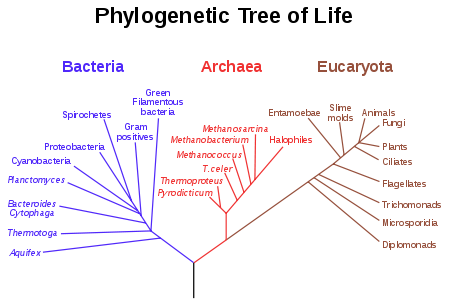
\includegraphics[width=4in]{images/dendrogram.png}
\caption{Example of a dendrogram.}
\end{figure}

The following algorithm is a hierarchical clustering algorithm with the following characteristics:

\begin{itemize}
\item Individual points do not need to be vectors (although they can be).
\item Points may have a weight used to determine their relative importance in identifying the characteristics of the cluster (think of clustering financial assets based on the time series of their returns; the weight could the average traded volume).
\item The distance between points is computed by a metric function provided by the user. The metric can return {\ft None} if there is no known connection between two points.
\item The algorithm can be used to build the entire {\it dendrogram} \index{dendrogram}, or it can stop for a given value of $k$, a target number of clusters.
\item For points that are vectors and a given $k$, the result is similar to the result of the $k$-means clustering.
\end{itemize}

The algorithm works like any other hierarchical clustering algorithm. At the beginning, all-to-all distances are computed and stored in a list {\ft d}. Each point is its own cluster. At each iteration, the two clusters closer together are merged to form one bigger cluster. The distance between each other cluster and the merged cluster is computed by performing a weighted average of the distances between the other cluster and the two merged clusters. The weight factors are provided as input. This is equivalent to what the $k$-means algorithm does by computing the position of a centroid based on the vectors of the member points.

The algorithm {\ft self.q} implements disjointed sets representing the set of clusters. The algorithm {\ft self.q} is a dictionary. If {\ft self.q[i]} is a list, then {\ft i} is its own cluster, and the list contains the IDs of the member points. If  {\ft self.q[i]} is an integer, then cluster {\ft i} is no longer its own cluster as it was merged to the cluster represented by the integer.

At each point in time, each cluster is represented by one element, which can be found recursively by {\ft self.parent(i)}. This function returns the ID of the cluster containing element {\ft i} and returns a list of IDs of all points in the same cluster:

\index{class!Cluster}

%%% META:FILE:nlib/cluster.nim
\begin{lstlisting}[caption={in file: {\ft nlib/cluster.nim}}]
type
  ClusterEntry = object
    case isList: bool
    of true: members: seq[int]
    of false: parentId: int

  Cluster*[T] = ref object
    points*: seq[T]
    metric*: proc(a, b: T): float
    k*: int
    w*: seq[float]
    q*: Table[int, ClusterEntry]
    d*: seq[(float, int, int)]
    dd*: seq[(float, int)]
    r*: float
    v*: seq[seq[int]]

proc newCluster*[T](points: seq[T],
                    metric: proc(a, b: T): float,
                    weights: seq[float] = @[]): Cluster[T] =
  result = Cluster[T](points: points, metric: metric, k: points.len)
  result.w = if weights.len > 0: weights
             else: newSeqWith(points.len, 1.0)
  for i in 0 ..< points.len:
    result.q[i] = ClusterEntry(isList: true, members: @[i])
  for i in 0 ..< points.len:
    for j in i + 1 ..< points.len:
      let m = metric(points[i], points[j])
      if not m.isNaN:
        result.d.add (m, i, j)
  result.d.sort()

proc parent*[T](c: Cluster[T], i: int): (int, seq[int]) =
  var i = i
  while c.q[i].isList == false:
    i = c.q[i].parentId
  (i, c.q[i].members)

proc step*[T](c: Cluster[T]): (float, seq[seq[int]]) =
  if c.k > 1:
    let head = c.d[0]
    c.r = head[0]
    var i = head[1]
    var j = head[2]
    c.d.delete(0)
    let (pi, x) = c.parent(i)
    let (pj, y) = c.parent(j)
    var merged = x & y
    c.q[pi] = ClusterEntry(isList: true, members: merged)
    c.q[pj] = ClusterEntry(isList: false, parentId: pi)
    dec c.k
    var newD: seq[(float, int, int)] = @[]
    var oldD = initTable[int, (float, float)]()
    for (r, h, k) in c.d:
      if h in [pi, pj]:
        let (a, b) = oldD.getOrDefault(k, (0.0, 0.0))
        oldD[k] = (a + c.w[k] * r, b + c.w[k])
      elif k in [pi, pj]:
        let (a, b) = oldD.getOrDefault(h, (0.0, 0.0))
        oldD[h] = (a + c.w[h] * r, b + c.w[h])
      else:
        newD.add (r, h, k)
    for k, ab in tables.pairs(oldD):
      newD.add (ab[0] / ab[1], pi, k)
    newD.sort()
    c.d = newD
    c.w[pi] = c.w[pi] + c.w[pj]
    var v: seq[seq[int]] = @[]
    for _, e in tables.pairs(c.q):
      if e.isList: v.add e.members
    c.v = v
    c.dd.add (c.r, c.v.len)
  (c.r, c.v)

proc find*[T](c: Cluster[T], k: int): (float, seq[seq[int]]) =
  while c.k > k:
    discard c.step()
  (c.r, c.v)
\end{lstlisting}

Given a set of points, we can determine the most likely number of clusters representing the data, and we can make a plot of the number of clusters versus distance and look for a plateau in the plot. In correspondence with the plateau, we can read from the $y$-coordinate the number of clusters. This is done by the function {\ft cluster} in the preceding algorithm, which returns the average distance between clusters and a list of clusters.

For example:

\begin{lstlisting}
proc metric(a, b: seq[float]): float =
  for i in 0 ..< a.len: result += (a[i] - b[i]) ^ 2
  result = sqrt(result)

randomize()
var points: seq[seq[float]] = @[]
for i in 0 ..< 200:
  var p = newSeq[float](10)
  for j in 0 ..< 10:
    p[j] = gauss(float(i mod 5), 0.3)
  points.add p
let c = newCluster[seq[float]](points, metric)
let (r, clusters) = c.find(1)
# Render the dendrogram using `savePlot` on (distance, count).
\end{lstlisting}

With our sample data, we obtain the following plot (``clustering1.png''):

\begin{figure}[ht]
\centering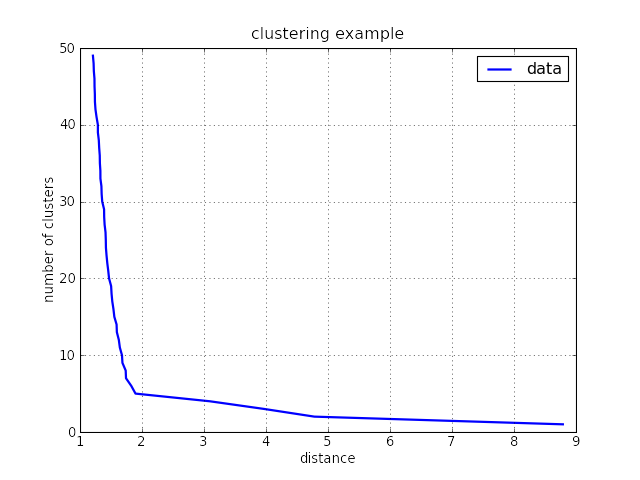
\includegraphics[width=4in]{images/clustering1.png}
\caption{Number of clusters found as a function of the distance cutoff.}
\end{figure}

and the location where the curve bends corresponds to five clusters. Although our points live in 10 dimensions, we can try to project them into two dimensions and see the five clusters (``clustering2.png''):

\begin{figure}[ht]
\centering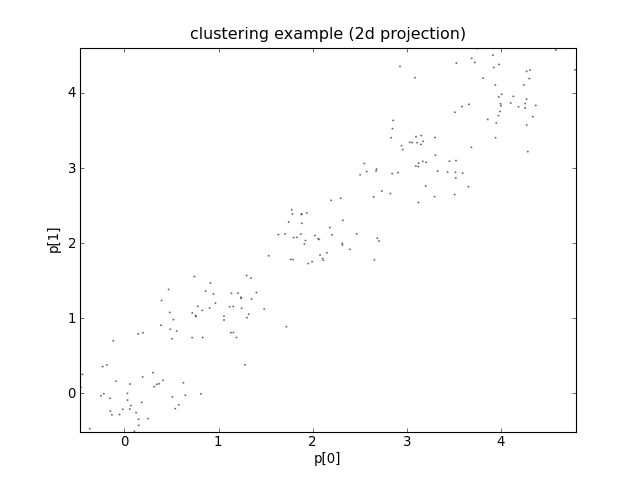
\includegraphics[width=4in]{images/clustering2.png}
\caption{Visual representation of the clusters where the points coordinates are projected in 2D.}
\end{figure}

\goodbreak\subsection{Neural network}

\index{neural network}

An artificial {\it neural network} is an electrical circuit (usually simulated in software) that mimics the functionality of the neurons in the animal (and human) brain~\cite{neural}. It is usually employed in pattern recognition. The network consists of a set of simulated neurons, connected by links (synapses). Some links connect the neurons with each other, some connect the neurons with the input and some with the output. Neurons are usually organized in the layers with one {\it input layer} of neurons connected only with the input and the next layer.  Another one, the {\it output layer}, comprises neurons connected only with the output and previous layers, or many {\it hidden layers} of neurons connected only with other neurons.
Each neuron is characterized by input links and output links. Each output of a neuron is a function of its inputs. The exact shape of that function depends on the network and on parameters that can be adjusted. Usually this function is chosen to be a monotonic increasing function on the sum of the inputs, where both the inputs and the outputs take values in the [0, 1] range. The inputs can be thought as electrical signals reaching the neuron. The output is the electrical signal emitted by the neuron. Each neuron is defined by a set of parameters {\ft a} which determined the relative weight of the input signals. A common choice for this characteristic function is:

\begin{equation}
\textrm{output}_{ij} = \tanh(\sum_k a_{ijk} \textrm{input}_{ik})
\end{equation}

where $i$ labels the neuron, $j$ labels the output, $k$ labels the input, and $a_{ijk}$ are characteristic parameters describing the neurons.

The network is trained by providing an input and adjusting the characteristics $a_{ijk}$ of each neuron $k$ to produce the expected output. The network is trained iteratively until its parameters converge (if they converge), and then it is ready to make predictions. We say the network has learned from the training data set.

\begin{figure}[ht]
\centering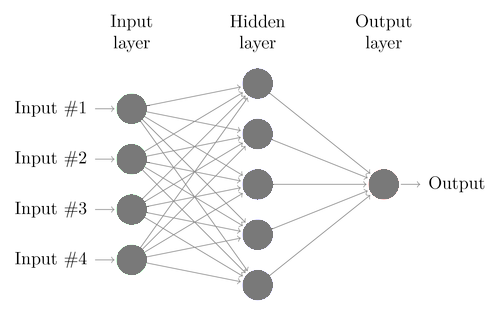
\includegraphics[width=4in]{images/neural.png}
\caption{Example of a minimalist neural network.}
\end{figure}

\index{class!NeuralNetwork}

%%% META:FILE:nlib/neural.nim
\begin{lstlisting}[caption={in file: {\ft nlib/neural.nim}}]
type
  NeuralNetwork* = ref object
    ni*, nh*, no*: int
    ai*, ah*, ao*: seq[float]
    wi*, wo*: Matrix       # weights
    ci*, co*: Matrix       # last weight change (momentum)

proc nnRand(a, b: float): float = (b - a) * rand(1.0) + a
proc sigmoid(x: float): float = tanh(x)
proc dsigmoid(y: float): float = 1.0 - y * y

proc newNeuralNetwork*(ni, nh, no: int): NeuralNetwork =
  result = NeuralNetwork(
    ni: ni + 1,    # +1 for bias node
    nh: nh,
    no: no,
    ai: newSeqWith(ni + 1, 1.0),
    ah: newSeqWith(nh, 1.0),
    ao: newSeqWith(no, 1.0),
    wi: newMatrix(ni + 1, nh,
                  proc(r, c: int): float = nnRand(-0.2, 0.2)),
    wo: newMatrix(nh, no,
                  proc(r, c: int): float = nnRand(-2.0, 2.0)),
    ci: newMatrix(ni + 1, nh),
    co: newMatrix(nh, no))

proc update*(n: NeuralNetwork, inputs: seq[float]): seq[float] =
  if inputs.len != n.ni - 1:
    raise newException(ValueError, "wrong number of inputs")
  for i in 0 ..< n.ni - 1:
    n.ai[i] = inputs[i]
  for j in 0 ..< n.nh:
    var s = 0.0
    for i in 0 ..< n.ni: s += n.ai[i] * n.wi[i, j]
    n.ah[j] = sigmoid(s)
  for k in 0 ..< n.no:
    var s = 0.0
    for j in 0 ..< n.nh: s += n.ah[j] * n.wo[j, k]
    n.ao[k] = sigmoid(s)
  result = n.ao

proc backPropagate*(n: NeuralNetwork, targets: seq[float],
                    N, M: float): float =
  if targets.len != n.no:
    raise newException(ValueError, "wrong number of target values")
  var outputDeltas = newSeq[float](n.no)
  for k in 0 ..< n.no:
    let error = targets[k] - n.ao[k]
    outputDeltas[k] = dsigmoid(n.ao[k]) * error
  var hiddenDeltas = newSeq[float](n.nh)
  for j in 0 ..< n.nh:
    var error = 0.0
    for k in 0 ..< n.no: error += outputDeltas[k] * n.wo[j, k]
    hiddenDeltas[j] = dsigmoid(n.ah[j]) * error
  for j in 0 ..< n.nh:
    for k in 0 ..< n.no:
      let change = outputDeltas[k] * n.ah[j]
      n.wo[j, k] = n.wo[j, k] + N * change + M * n.co[j, k]
      n.co[j, k] = change
  for i in 0 ..< n.ni:
    for j in 0 ..< n.nh:
      let change = hiddenDeltas[j] * n.ai[i]
      n.wi[i, j] = n.wi[i, j] + N * change + M * n.ci[i, j]
      n.ci[i, j] = change
  var error = 0.0
  for k in 0 ..< targets.len:
    error += 0.5 * (targets[k] - n.ao[k]) ^ 2
  return error

proc test*(n: NeuralNetwork, patterns: seq[(seq[float], seq[float])]) =
  for p in patterns:
    echo p[0], " -> ", n.update(p[0])

proc weights*(n: NeuralNetwork) =
  echo "Input weights:"
  for i in 0 ..< n.ni:
    var row: seq[float]
    for j in 0 ..< n.nh: row.add n.wi[i, j]
    echo row
  echo ""
  echo "Output weights:"
  for j in 0 ..< n.nh:
    var row: seq[float]
    for k in 0 ..< n.no: row.add n.wo[j, k]
    echo row

proc train*(n: NeuralNetwork,
            patterns: seq[(seq[float], seq[float])],
            iterations = 1000, N = 0.5, M = 0.1,
            check = false) =
  for i in 0 ..< iterations:
    var error = 0.0
    for p in patterns:
      discard n.update(p[0])
      error += n.backPropagate(p[1], N, M)
    if check and i mod 100 == 0:
      echo "error ", error
\end{lstlisting}

In the following example, we teach the network the XOR function, and we create a network with two inputs, two intermediate neurons, and one output. We train it and check what it learned:

\begin{lstlisting}
let pat = @[(@[0.0, 0.0], @[0.0]),
            (@[0.0, 1.0], @[1.0]),
            (@[1.0, 0.0], @[1.0]),
            (@[1.0, 1.0], @[0.0])]
let n = newNeuralNetwork(2, 2, 1)
n.train(pat)
n.test(pat)
# @[0.0, 0.0] -> @[0.00...]
# @[0.0, 1.0] -> @[0.98...]
# @[1.0, 0.0] -> @[0.98...]
# @[1.0, 1.0] -> @[-0.00...]
\end{lstlisting}

Now, we use our neural network to learn patterns in stock prices and predict the next day return. We then check what it has learned, comparing the sign of the prediction with the sign of the actual return for the same days used to train the network:
%%% META:FILE:test.nim
\begin{lstlisting}[caption={in file: {\ft test.nim}}]
let storage = newPersistentDictionary("sp100.json")
var v: seq[float] = @[]
for day in storage["AAPL/2011"][1 .. ^1]:
  v.add day["arithmetic_return"].getFloat * 300.0
var pat: seq[(seq[float], seq[float])] = @[]
for i in 0 ..< v.len - 5:
  pat.add (v[i ..< i + 5], @[v[i + 5]])
let n = newNeuralNetwork(5, 5, 1)
n.train(pat)
var predictions: seq[seq[float]] = @[]
for item in pat: predictions.add n.update(item[0])
var hits = 0.0
for i, e in predictions:
  if e[0] * v[i + 5] > 0: hits += 1.0
let successRate = hits / float(pat.len)
\end{lstlisting}
The learning process depends on the random number generator; therefore, sometimes, for this small training data set, the network succeeds in predicting the sign of the next day arithmetic return of the stock with more than 50\% probability, and sometimes it does not. We leave it to the reader to study the significance of this result but using a different subset of the data for the training of the network and for testing its success rate.

\goodbreak\subsection{Genetic algorithms}

\index{genetic algorithms}

Here we consider a simple example of genetic algorithms~\cite{barricelli}.

We have a population of chromosomes in which each chromosome is just a data structure, in our example, a string of random ``ATGC'' characters.

We also have a metric to measure the fitness of each chromosome.

At each iteration, only the top-ranking chromosomes in the population survive. The top 10 mate with each other, and their offspring constitute the population for the next iteration. When two members of the population mate, the newborn member of the population has a new DNA sequence, half of which comes from the father and half from the mother, with two randomly mutated DNA basis.

The algorithm stops when we reach a maximum number of generations or we find a chromosome of the population with maximum fitness.

In the following example, the fitness is measured by the similarity between a chromosome and a random target chromosome. The population evolves to approximate better and better that one random target chromosome:

\index{class!Chromosome}

%%% META:FILE:genetic.nim
\begin{lstlisting}[caption={in file: {\ft genetic.nim}}]
import std/[random, algorithm, sequtils]

const
  ALPHABET = "ATGC"
  SIZE = 32
  MUTATIONS = 2

type
  Chromosome* = ref object
    dna*: string

proc randomChar(): char = ALPHABET[rand(ALPHABET.len - 1)]

proc newChromosome*(): Chromosome =
  result = Chromosome(dna: newString(SIZE))
  for i in 0 ..< SIZE: result.dna[i] = randomChar()

proc newChromosome*(father, mother: Chromosome): Chromosome =
  result = Chromosome(
    dna: father.dna[0 ..< SIZE div 2] & mother.dna[SIZE div 2 .. ^1])
  for _ in 0 ..< MUTATIONS:
    result.dna[rand(SIZE - 1)] = randomChar()

proc fitness*(c, target: Chromosome): int =
  for i, ch in c.dna:
    if ch == target.dna[i]: inc result

proc top*(population: seq[Chromosome], target: Chromosome,
          n = 10): seq[Chromosome] =
  var table: seq[(int, Chromosome)] = @[]
  for chromo in population:
    table.add (chromo.fitness(target), chromo)
  table.sort(proc(a, b: (int, Chromosome)): int = cmp(b[0], a[0]))
  for i in 0 ..< min(n, table.len):
    result.add table[i][1]

proc oneof*(population: seq[Chromosome]): Chromosome =
  population[rand(population.len - 1)]

proc main() =
  const GENERATIONS = 10000
  const OFFSPRING = 20
  const SEEDS = 20
  let target = newChromosome()

  var population: seq[Chromosome] = @[]
  for _ in 0 ..< SEEDS: population.add newChromosome()
  for i in 0 ..< GENERATIONS:
    echo "\n\nGENERATION: ", i
    echo 0, " ", target.dna
    let fittest = top(population, target)
    for chromosome in fittest: echo i, " ", chromosome.dna
    var best = 0
    for chromo in fittest: best = max(best, chromo.fitness(target))
    if best == SIZE:
      echo "SOLUTION FOUND"
      break
    population = @[]
    for _ in 0 ..< OFFSPRING:
      population.add newChromosome(oneof(fittest), oneof(fittest))

when isMainModule:
  randomize()
  main()
\end{lstlisting}

Notice that this algorithm can easily be modified to accommodate other fitness metrics and DNA that consists of a data structure other than a sequence of ``ATGC'' symbols. The only trickery is finding a proper mating algorithm that preserves some of the fitness features of the parents in the DNA of their offspring. If this does not happen, each next generation loses the fitness properties gained by its parents, thus causing the algorithm not to converge. In our case, it works because if the parents are ``close'' to the target, then half of the DNA of each parent is also close to the corresponding half of the target DNA. Therefore the DNA of the offspring is as fit as the average of their parents. On top of this, the two random mutations allow the algorithm to further explore the space of all possible DNA sequences.

\goodbreak\section{Long and infinite loops}
\index{P}\index{NP}\index{NPC}\index{EXP}
\goodbreak\subsection{P, NP, and NPC}

We say a problem is in P if it can be solved in polynomial time: $%
T_{worst}\in O(n^\alpha )$ for some $\alpha $.

We say a problem is in NP if an input string can be verified to be a
solution in polynomial time: $T_{worst}\in O(n^\alpha )$ for some $\alpha $.

We say a problem is in co-NP if an input string can be verified not to be a
solution in polynomial time: $T_{worst}\in O(n^\alpha )$ for some $\alpha $.

We say a problem is in NPH (NP Hard) if it is harder than any other problem
in NP.

We say a problem is in NPC (NP Complete) if it is in NP and in NPH.
Consequences:
\begin{equation}
\text{if }\exists x\text{ }|\text{ }x\in NPC\text{ and }x\in P\Rightarrow
\forall y\in NP, y\in P
\end{equation}

There are a number of open problems about the relations among these sets.
Is the set co-NP equivalent to NP? Or perhaps is the intersection between co-NP and NP equal to P?
Are NP and NPC the same set? These questions are very important in computer science because if, for example, NP turns out to be the same set as NPC, it means that it must be possible to find algorithms that solve in polynomial time problems that currently do not have a polynomial time solution. Conversely, if one could prove that NP is not equivalent to NPC, we would know that a polynomial time solution to NPC problems does not exist~\cite{pnp}.

\subsection{Cantor"s argument}

\index{Cantor"s argument}

Cantor proved that the real numbers in any interval (e.g., in $[0, 1)$)
are more than the integer numbers, therefore real numbers are uncountable~\cite{hofstadter}.
The proof proceeds as follows:

\begin{enumerate}
\item  Consider the real numbers in the interval $[0, 1)$ not including 1$.$

\item  Assume that these real numbers are countable. Therefore it is
possible to associate each of them to an integer
\begin{equation}
\begin{tabular}{lll}
1 & $\longleftrightarrow $ & $0.xxxxxxxxxxx...$ \\
2 & $\longleftrightarrow $ & $0.xxxxxxxxxxx...$ \\
3 & $\longleftrightarrow $ & $0.xxxxxxxxxxx...$ \\
4 & $\longleftrightarrow $ & $0.xxxxxxxxxxx...$ \\
5 & $\longleftrightarrow $ & $0.xxxxxxxxxxx...$ \\
... & ... & ...
\end{tabular}
\label{cantor}
\end{equation}
(here $x$ represent a decimal digit of a real numbers)

\item  Now construct a number $\alpha =0.yyyyyyyy....$ where the first
decimal digit differs from the first decimal digit of the first real number
of table \ref{cantor}, the second decimal digit differs from the second
decimal digit of the second real number of table \ref{cantor}, and so on and
so on for all the infinite decimal digits:
\begin{equation}
\begin{tabular}{lll}
1 & $\longleftrightarrow $ & $0.\overline{x}xxxxxxxxxx...$ \\
2 & $\longleftrightarrow $ & $0.x\overline{x}xxxxxxxxx...$ \\
3 & $\longleftrightarrow $ & $0.xx\overline{x}xxxxxxxx...$ \\
4 & $\longleftrightarrow $ & $0.xxx\overline{x}xxxxxxx...$ \\
5 & $\longleftrightarrow $ & $0.xxxx\overline{x}xxxxxx...$ \\
... & ... & ...
\end{tabular}
\label{cantor2}
\end{equation}

\item  The new number $\alpha $ is a real number, and by construction, it is
not in the table. In fact, it differs with each item by at least one decimal
digit. Therefore the existence of $\alpha $ disproves the assumption that
all real numbers in the interval $[0, 1)$ are listed in the table.
\end{enumerate}

There is a very practical consequence of this argument. In fact, in chapter 2, we have seen the distinction between type {\ft float} and class {\ft Decimal}. We have seen about pitfalls of {\ft float} and how {\ft Decimal} can represent floating point numbers with arbitrary precision (assuming we have the memory to do so). Cantor"s argument tells us there are numbers that cannot even be represented as {\ft Decimal} because they would require an infinite amount of storage; $\pi$ and $e$ are examples of these numbers.

\subsection{G\"odel"s theorem}

\index{G\"odel"s theorem}

G\"odel used a similar diagonal argument to prove that there are as many
problems (or theorems) as real numbers and as many algorithms (or proofs) as
natural numbers~\cite{hofstadter}. Because there is more of the former than the latter, it
follows that there are problems for which there is no corresponding solving
algorithm. Another interpretation of G\"odel"s theorem is that, in any formal
language, for example, mathematics, there are theorems that cannot be proved.

Another consequence of G\"odel"s theorem is the following:
it is impossible to write a computer program to test if a given algorithm
stops or enters into an infinite loop.

Consider the following code:

\begin{lstlisting}
import std/sets

proc next(i: int) =
  var i = i
  while toHashSet($($(i * i))).card > 2:
    i += 2
  echo i

next(81621)
\end{lstlisting}

This code check searches for a number equal or greater than 81621 whose square is comprised of only two digits. 
Nobody knows whether such number exists, therefore nobody knows if this code stops.

Although one day this problem may be solved, there are many other problems that
are still unsolved; actually, there are an infinite number of them.

\chapter{Numerical Algorithms}

\goodbreak\section{Well-posed and stable problems}

\index{well-posed problems}
\index{stable problems}

Numerical algorithms deal mostly with well-posed and stable problems.

A problem is well posed if
\begin{itemize}
\item The solution exists and is unique
\item The solution has a continuous dependence on input data (a small change in the input causes a small change in the output)
\end{itemize}

\index{critical points}\index{chaos}

Most physical problems are well posed, except at {\it critical points}, where any infinitesimal variation in one of the input parameters of the system can cause a large change in the output and therefore in the behavior of the system. This is called {\it chaos}.

Consider the case of dropping a ball on a triangular-shaped mountain. Let the input of the problem be the horizontal position where the drop occurs and the output the horizontal position of the ball after a fixed amount of time. Almost anywhere the ball is dropped, it will roll down the mountain following deterministic and classical laws of physics, thus the position is calculable and a continuous function of the input position. This is true everywhere, except when the ball is dropped on top of the peak of the mountain. In this case, a minor infinitesimal variation to the right or to the left can make the ball roll to the right or to the left, respectively.  Therefore this is not a well posed problem.

A problem is said to be {\it stable} if the solution is not just continuous but also weakly sensitive to input data. This means that the change of the output (in percent) is smaller than the change in the input (in percent).

Numerical algorithms work best with stable problems.

We can quantify this as follows. Let $x$ be an input and $y$ be the output of a function:
\begin{equation}
y = f(x)
\end{equation}
We define the condition number of $f$ in $x$ as

\index{condition number}

\begin{equation}
\func{cond}(f, x) \equiv \frac{|dy/y|}{|dx/x|} = |x f'(x)/f(x)|
\end{equation}
(the latter equality only holds if $f$ is differentiable in $x$).

A problem with a low condition number is said to be well-conditioned, while a problem with a high condition number is said to be ill-conditioned. XXX

We say that a problem characterized by a function $f$ is well conditioned in a domain $D$ if the condition number is less than 1 for every input in the domain. We also say that a problem is stable if it is well conditioned.

In this book, we are mostly concerned with stable (well-conditioned) problems. If a problem is well-conditioned in for all input in a domain, it is also stable.


\goodbreak\section{Approximations and error analysis}

\index{error analysis}

Consider a physical quantity, for example, the length of a nail. Given one nail, we can measure its length by choosing a measuring instrument. Whatever instrument we choose, we will be able to measure the length of the nail within the resolution of the instrument. For example, with a tape measure with a resolution of 1 mm, we will only be able to determine the length of the nail within 1 mm of resolution. Repeated measurements performed at different times, by different people, using different instruments may bring different results. We can choose a more precise instrument, but it would not change the fact that different measures will bring different values compatible with the resolution of the instrument. Eventually one will have to face the fact that there may not be such a thing as the length of a nail. For example, the length varies with the temperature and the details of how the measurement is performed. In fact, a nail (as everything else) is made out of atoms, which are made of protons, neutrons, and electrons, which determine an electromagnetic cloud that fluctuates in space and time and depends on the surrounding objects and interacts with the instrument of measure. The length of the nail is the result of a measure.

For each measure there is a result, but the results of multiple measurements are not identical. The results of many measurements performed with the same resolution can be summarized in a distribution of results. This distribution will have a mean $\bar x$ and a standard deviation $\delta x$, which we call uncertainty. From now on, unless otherwise specified, we assume that the distribution of results is Gaussian so that $\bar x$ can be interpreted as the mean and $\delta x$ as the standard deviation.

Now let us consider a system that, given an input $x$, produces the output $y$; $x$ and $y$ are physical quantities that we can measure, although only with a finite resolution. We can model the system with a function $f$ such that $y = f(x)$ and, in general, $f$ is not known.

We have to make various approximations:
\begin{itemize}
\item We can replace the ``true'' value for the input with our best estimate, $\bar x$, and its associated uncertainty, $\delta x$.

\item We can replace the ``true'' value for the output with our best estimate, $\bar y$, and its associated uncertainty, $\delta y$.

\item Even if we know there is a ``true'' function $f$ describing the system, our implementation for the function is always an approximation, $\bar f$. In fact,  we may not have a single approximation but a series of approximations of increasing precision, $f_n$, which become more and more accurate (usually) as $n$ increases. If we are lucky, up to precision errors, as $n$ increases, our approximations will become closer and closer to $f$, but this will take an infinite amount of time. We have to stop at some finite $n$.
\end{itemize}

\index{data error}\index{computational error}\index{statistical error}\index{systematic error}\index{total error}\index{propagated data error}

With the preceding definition, we can define the following types of errors:

\begin{itemize}
\item {\bf Data error}: the difference between $x$ and $\bar x$.

\item {\bf Computational error}: the difference between $\bar f(\bar x)$ and $y$.
Computational error includes two parts systematic error and statistical error.

\item {\bf Statistical error}: due to the fact that, often, the computation of $\bar f(x) = \lim_{n\rightarrow\infty} f_n(x)$ is too computationally expensive and we must approximate $\bar f(x)$ with $f_n(x)$. This error can be estimated and controlled.

\item {\bf Systematic error}: due to the fact that $\bar f(x) = \lim_{n\rightarrow\infty} f_n(x) \neq f(x)$. This is for two reasons: modeling errors (we do not know $f(x)$) and rounding errors (we do not implement $f(x)$ with arbitrary precision arithmetics).

\item {\bf Total error}: defined as the computational error + the propagated data error and in a formula:
\begin{equation}
\delta y = |f(\bar x)-f_n(\bar x)| + |f'_n(\bar x)|\delta x
\end{equation}
The first term is the computational error (we use $f_n$ instead of the true $f$), and the second term is the propagated data error ($\delta x$, the uncertainty in $x$, propagates through $f_n$).
\end{itemize}


\goodbreak\subsection{Error propagation}

\index{error propagation}

When a variable $x$ has a finite Gaussian uncertainty $\delta x$, how does the uncertainty propagate through a function $f$? Assuming the uncertainty is small, we can always expand using a Taylor series:

\begin{equation}
y+\delta y = f(x+\delta x) = f(x) + f'(x)\delta x + O(\delta x^2)
\end{equation}
And because we interpret $\delta y$ as the width of the distribution $y$, it should be positive:
\begin{equation}
  \delta y = |f'(x)|\delta x
\end{equation}

We have used this formula before for the propagated data error.
For functions of two variables $z = f(x, y)$ and assuming the uncertainties in $x$ and $y$ are independent, 

\begin{equation}
  \delta z = \sqrt{\left|\frac{\partial f(x, y)}{\partial x}\right|^2\delta x^2 +
\left|\frac{\partial f(x, y)}{\partial y}\right|^2\delta y^2 }
\end{equation}

which for simple arithmetic operations reduces to

\begin{tabular}{ll}
  $z = x + y$ &
  $\delta z = \sqrt{\delta x^2 + \delta y^2 }$ \\
  $z = x - y$ &
  $\delta z = \sqrt{\delta x^2 + \delta y^2 }$ \\
  $z = x * y$ &
  $\delta z = |x * y|\sqrt{(\delta x/x)^2 + (\delta y/y)^2 }$ \\
  $z = x / y$ &
  $\delta z = |x/y|\sqrt{(\delta x/x)^2 + (\delta y/y)^2 }$ \\
\end{tabular}

Notice that when $z=x-y$ approaches zero, the uncertainty in $z$ is larger than the uncertainty in $x$ and $y$ and can overwhelm the result.
Also notice that if $z=x/y$ and $y$ is small compared to $x$, then the uncertainty in $z$ can be large.
Bottom line: try to avoid differences between numbers that are in proximity of each other and try to avoid dividing by small numbers.

\goodbreak\section{Standard strategies}

Here are some strategies that are normally employed in numerical algorithms:

\begin{itemize}
\item Approximate a continuous system with a discrete system
\item Replace integrals with sums
\item Replace derivatives with finite differences
\item Replace nonlinear with linear + corrections
\item Transform a problem into a different one
\item Approach the true result by iterations
\end{itemize}

Here are some examples of each of the strategies.

\goodbreak\subsection{Approximate continuous with discrete}

Consider a ball in a one-dimensional box of size $L$, and let $x$ be the position of the ball in the box. Instead of treating $x$ as a continuous variable, we can assume a finite resolution of $h = L/n$ (where $h$ is the minimum distance we can distinguish without instruments and $n$ is the maximum number of distinct discrete points we can discriminate), and set $x \equiv h i$, where $i$ is an integer in between $0$ and $n$; $x=0$ when $i=0$ and $x=L$ when $i=n$.


\goodbreak\subsection{Replace derivatives with finite differences}

\index{derivative}\index{finite differences}

Computing $\textrm{d}f(x)/\textrm{d}x$ analytically is only possible when the function $f$ is expressed in simple analytical terms. Computing it analytically is not possible when $f(x)$ is itself implemented as a numerical algorithm. Here is an example:

\begin{lstlisting}
proc f(x: float): float =
  var s = 1.0
  var t = 1.0
  for i in 1 ..< 10:
    (s, t) = (s + t, t * x / float(i))
  return s
\end{lstlisting}

What is the derivative of $f(x)$?

The most common ways to define a derivative are the right derivative

\begin{equation}
  \frac{\textrm{d}f^{+}(x)}{\textrm{d}x} = \lim_{h\rightarrow 0}
  \frac{f(x+h)-f(x)}{h}
\end{equation}
the left derivative
\begin{equation}
  \frac{\textrm{d}f^{-}(x)}{\textrm{d}x} = \lim_{h\rightarrow 0}\
  \frac{f(x)-f(x-h)}{h}
\end{equation}
and the average of the two
\begin{equation}
  \frac{\textrm{d}f(x)}{\textrm{d}x} = \frac12\left(
  \frac{\textrm{d}f^{+}(x)}{\textrm{d}x} +
  \frac{\textrm{d}f^{-}(x)}{\textrm{d}x} \right) =
  \lim_{h\rightarrow 0}\frac{f(x+h)-f(x-h)}{2h}
\end{equation}

If the function is differentiable in $x$, then, by definition of ``differentiable, '' the left and right definitions are equal, and the three prior definitions are equivalent. We can pick one or the other, and the difference will be a systematic error.

If the limit exists, then it means that

\begin{equation}
\frac{\textrm{d}f(x)}{\textrm{d}x} = \frac{f(x+h)-f(x-h)}{2h} + O(h)
\end{equation}

where $O(h)$ indicates a correction that, at most, is proportional to $h$.

The three definitions are equivalent for functions that are differentiable in $x$, and the latter is preferable because it is more symmetric.

Notice that even more definitions are possible as long as they agree in the limit $h\rightarrow 0$. Definitions that converge faster as $h$ goes to zero are referred to as ``improvement.''


\index{functional}

We can easily implement the concept of a numerical derivative in code by creating a {\it functional} $D$ that takes a function $f$ and returns the function $\frac{\textrm{d}f(x)}{\textrm{d}x}$ (a functional is a function that returns another function):

%%% META:FILE:nlib/calculus.nim
\begin{lstlisting}[caption={in file: {\ft nlib/calculus.nim}}]
proc D*(f: proc(x: float): float, h = 1e-6): proc(x: float): float =
  result = proc(x: float): float = (f(x + h) - f(x - h)) / 2.0 / h
\end{lstlisting}

We can do the same with the second derivative:

\begin{equation}
  \frac{\textrm{d}^2f(x)}{\textrm{d}x^2} = \frac{f(x+h)-2f(x)-f(x-h)}{h^2} + O(h)
\end{equation}

%%% META:FILE:nlib/calculus.nim
\begin{lstlisting}[caption={in file: {\ft nlib/calculus.nim}}]
proc DD*(f: proc(x: float): float, h = 1e-6): proc(x: float): float =
  result = proc(x: float): float =
    (f(x + h) - 2.0 * f(x) + f(x - h)) / (h * h)
\end{lstlisting}

Here is an example:

\begin{lstlisting}
proc f(x: float): float = x * x - 5.0 * x
echo f(0.0)            # 0.0
let f1 = D(f)          # first derivative
echo f1(0.0)           # -5.0
let f2 = DD(f)         # second derivative
echo f2(0.0)           # 2.00000...
let f2b = D(f1)        # second derivative (composing)
echo f2b(0.0)          # 1.99999...
\end{lstlisting}

Notice how composing the first derivative twice or computing the second derivative directly yields a similar result.

We could easily derive formulas for higher-order derivatives and implement them, but they are rarely needed.

\goodbreak\subsection{Replace nonlinear with linear}

\index{linear approximation}

Suppose we are interested in the values of $f(x)=\sin(x)$ for values of $x$ between $0$ and $0.1$:

\begin{lstlisting}
import std/math
for i in 0 .. 10:
  let x = 0.01 * float(i)
  echo x, " ", sin(x), " ",
       formatFloat(abs(x - sin(x)) / sin(x) * 100, ffDecimal, 2)
# 0.01 0.009999833... 0.00
# 0.02 0.019998666... 0.01
# 0.03 0.029995500... 0.02
# 0.04 0.039989334... 0.03
# 0.05 0.049979169... 0.04
# 0.06 0.059964006... 0.06
# 0.07 0.069942847... 0.08
# 0.08 0.079914693... 0.11
# 0.09 0.089878549... 0.14
# 0.1 0.0998334166... 0.17
\end{lstlisting}
Here the first column is the value of $x$, the second column is the corresponding $\sin(x)$, and the third column is the relative difference (in percent) between $x$ and $\sin(x)$. The difference is always less than $20\%$; therefore, if we are happy with this precision, then we can replace $\sin(x)$ with $x$.

This works because any function $f(x)$ can be expanded using a Taylor series. The first order of the Taylor expansion is linear. For values of $x$ sufficiently close to the expansion point, the function can therefore be approximated with its Taylor expansion.

Expanding on the previous example, consider the following code:

\begin{lstlisting}
import std/math
for i in 0 .. 10:
  let x = 0.01 * float(i)
  let s = x - x * x * x / 6.0
  echo x, " ", sin(x), " ", s, " ",
       formatFloat(abs(s - sin(x)) / sin(x) * 100, ffDecimal, 6)
# 0.01 0.009999833... 0.009999... 0.000000
# 0.02 0.019998666... 0.019998... 0.000000
# 0.03 0.029995500... 0.029995... 0.000001
# 0.04 0.039989334... 0.039989... 0.000002
# 0.05 0.049979169... 0.049979... 0.000005
# 0.06 0.059964006... 0.059964... 0.000011
0.07 0.069942847... 0.069942... 0.000020
0.08 0.079914693... 0.079914... 0.000034
0.09 0.089878549... 0.089878... 0.000055
0.1 0.0998334166... 0.099833... 0.000083
\end{lstlisting}

Notice that the third column $s = x - x^3/6$ is very close to $\sin(x)$. In fact, the difference is less than one part in 10, 000 (fourth column). Therefore, for $x \in [-1, +1]$, it is possible to replace the $sin(x)$ function with the $x-x^3/6$ polynomial. Here we just went one step further in the Taylor expansion, replacing the first order with the third order. The error committed in this approximation is very small.


\goodbreak\subsection{Transform a problem into a different one}

Continuing with the previous example, the polynomial approximation for the sin function works when $x$ is smaller than $1$ but fails when $x$ is greater than or equal to $1$. In this case, we can use the following relations to reduce the computation of $\sin(x)$ for large $x$ to $\sin(x)$ for $0<x<1$. In particular, we can use

\begin{equation}
\sin(x) = -\sin(-x) \textrm{when} x < 0
\end{equation}

to reduce the domain to $x \in [0, \infty]$. We can then use

\begin{equation}
\sin(x) = \sin(x - 2k\pi) \qquad k\in \mathbb{N}
\end{equation}

to reduce the domain to $x \in [0, 2\pi)$

\begin{equation}
\sin(x) = -\sin(2\pi - x)
\end{equation}

to reduce the domain to $x \in [0, \pi)$

\begin{equation}
\sin(x) = \sin(\pi - x)
\end{equation}

to reduce the domain to $x \in [0, \pi/2)$, and

\begin{equation}
\sin(x) = \sqrt{1 - \sin(\pi/2 - x)^2}
\end{equation}

to reduce the domain to $x \in [0, \pi/4)$, where the latter is a subset of $[0, 1)$.

\goodbreak\subsection{Approximate the true result via iteration}

\index{approximations}

The approximations $\sin(x) \simeq x$ and $\sin(x) \simeq x - x^3/6$ came from linearizing the function $\sin(x)$ and adding a correction to the previous approximation, respectively. In general, we can iterate the process of finding corrections and approximating the true result.

Here is an example of a general iterative algorithm:
\begin{lstlisting}
result=guess
loop:
    compute correction
    result=result+correction
    if result sufficiently close to true result:
        return result
\end{lstlisting}

For the $\sin$ function:

\begin{lstlisting}
proc mysin(x: float): float =
  var s = 0.0
  var t = x
  var i = 3
  while i < 10:
    s += t
    t = -t * x * x / float(i) / float(i - 1)
    i += 2
  return s
\end{lstlisting}

Where do these formulas come from? How do we decide how many iterations we need? We address these problems in the next section.


\goodbreak\subsection{Taylor series}

\index{Taylor series}\index{Taylor Theorem}

A function $f(x):\mathbb{R}\rightarrow\mathbb{R}$ is said to be a {\it real analytical} in $\bar x$ if it is continuous in $x=\bar x$ and all its derivatives exist and are continuous in $x=\bar x$.

When this is the case, the function can be locally approximated with a local power series:

\begin{equation}
f(x) = f(\bar x) + f^{(0)}(\bar x)(x-\bar x) + ... + \frac{f^{(k)}(\bar x)}{n!}(x-\bar x)^k + R_k
\end{equation}

The remainder $R_k$ can be proven to be (Taylor"s theorem):
\begin{equation}
R_k = \frac{f^{(k+1)}(\xi)}{(k+1)!}(x-\bar x)^{k+1}
\end{equation}
where $\xi$ is a point in between $x$ and $\bar x$. Therefore, if $f^{(k+1)}$ exists and is limited within a neighborhood $D = \{x~\textrm{for}~|x-\bar x|<\epsilon\}$, then
\begin{equation}
|R_k| < \left| max_{x\in D} f^{(k+1)} \right| |(x-\bar x)^{k+1}|
\end{equation}

If we stop the Taylor expansion at a finite value of $k$, the preceding formula gives us the statistical error part of the computational error.

Some Taylor series are very easy to compute:

Exponential for $\bar x = 0$:

\begin{eqnarray}
f(x) &=& e^x \\
f^{(1)}(x) &=& e^x \\
... && ... \\
f^{(k)}(x) &=& e^x \\
e^x &=&  1 + x + \frac12 x^2 + ... + \frac1{k!}x^k + ...
\end{eqnarray}

Sin for $\bar x = 0$:

\begin{eqnarray}
f(x) &=& sin(x) \\
f^{(1)}(x) &=& cos(x) \\
f^{(2)}(x) &=& -sin(x) \\
f^{(3)}(x) &=& -cos(x) \\
... && ... \\
sin(x) &=&  x - \frac1{3!}x^3 + ... + \frac{(-1)^n}{(2k+1)!}x^{(2k+1)} + ...
\end{eqnarray}

We can show the effects of the various terms:

\begin{lstlisting}
var X: seq[float] = @[]
for i in 0 ..< 200: X.add 0.03 * float(i)

savePlot("images/sin.png", X, X.mapIt(sin(it)),
         title = "sin(x) approximations")
# Plot Taylor approximations on the same set of axes; in nlib.nim,
# `savePlot` accepts an optional list of additional curves.
\end{lstlisting}

\begin{figure}[ht]
\centering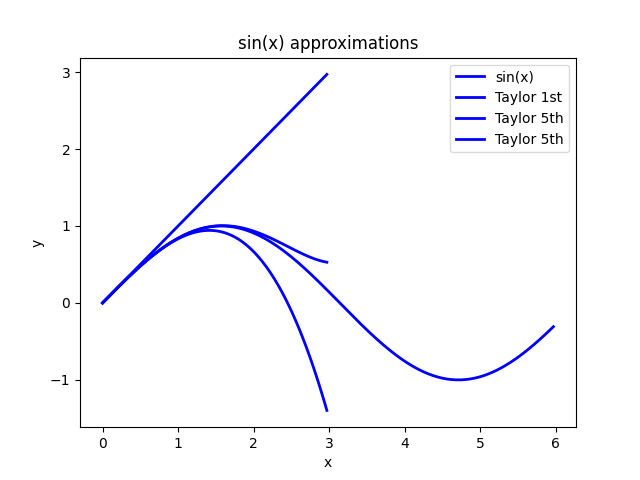
\includegraphics[width=4in]{images/sin.png}
\caption{The figure shows the $\sin$ function and its approximation using the Taylor expansion around $x=0$ at different orders.}
\end{figure}

Notice that we can very well expand in Taylor around any other point, for example, $\bar x = \pi/2$, and we get

\begin{equation}
sin(x) =  1 - \frac1{2}(x-\frac{\pi}{2})^2 + ... + \frac{(-1)^n}{(2k)!}(x-\frac{\pi}{2})^{(2k)} + ...
\end{equation}

and a plot would show:

\begin{lstlisting}
let a = PI / 2.0
var X: seq[float] = @[]
for i in 0 ..< 200: X.add 0.03 * float(i)
savePlot("images/sin2.png", X, X.mapIt(sin(it)),
         title = "sin(x) approximations")
# overlay Taylor expansions around `a` (orders 2, 4, 6) using
# the multi-curve form of `savePlot`.
\end{lstlisting}

\begin{figure}[ht]
\centering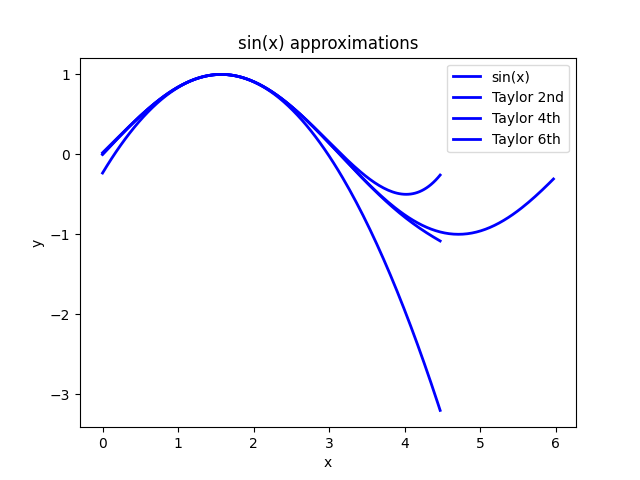
\includegraphics[width=4in]{images/sin2.png}
\caption{The figure shows the $\sin$ function and its approximation using the Taylor expansion around $x=\pi/2$ at different orders.}
\end{figure}

Similarly we can expand the $\cos$ function around $\bar x = 0$. Not accidentally, we would get the same coefficients as the Taylor expansion of the $\sin$ function around $\bar x = \pi/2$. In fact, $\sin(x) = \cos(x-\pi/2)$:

\begin{eqnarray}
f(x) &=& cos(x) \\
f^{(1)}(x) &=& -sin(x) \\
f^{(2)}(x) &=& -cos(x) \\
f^{(3)}(x) &=& sin(x) \\
... && ... \\
cos(x) &=&  1 - \frac1{2}x^2 + ... + \frac{(-1)^n}{(2k)!}x^{(2k)} + ...
\end{eqnarray}

With a simple replacement, it is easy to prove that
\begin{equation}
e^{ix} = \cos(x) + i \sin(x)
\end{equation}
which will be useful when we talk about Fourier and Laplace transforms.

Now let"s consider the $k$th term in Taylor expansion of $e^x$. It can be rearranged as a function of the previous $(k-1)-th$ term:

\begin{equation}
T_k(x) = \frac1{k!}x^n = \frac{x}{k} \frac1{(k-1)!}x^{k-1} = \frac{x}{k} T_{k-1}(x)
\end{equation}

For $x<0$, the terms in the sign have alternating sign and are decreasing in magnitude; therefore, for $x<0$, $R_k<T_{k+1}(1)$. This allows for an easy implementation of the Taylor expansion and its stopping condition:

%%% META:FILE:nlib/taylor.nim
\begin{lstlisting}[caption={in file: {\ft nlib/taylor.nim}}]
proc myexp*(x: float, precision = 1e-6, maxSteps = 40): float =
  if x == 0:
    return 1.0
  if x > 0:
    return 1.0 / myexp(-x, precision, maxSteps)
  var t = 1.0
  var s = 1.0
  for k in 1 ..< maxSteps:
    t = t * x / float(k)
    s = s + t
    if abs(t) < precision: return s
  raise newException(ArithmeticDefect, "no convergence")
\end{lstlisting}

This code presents all the features of many of the algorithms we see later in the chapter:
\begin{itemize}
\item It deals with the special case $e^0=1$.
\item It reduces difficult problems to easier problems (exponential of a positive number to the exponential of a negative number via $e^x = 1/e^{-x}$).
\item It approximates the ``true'' solution by iterations.
\item The max number of iterations is limited.
\item There is a stopping condition.
\item It detects failure to converge.
\end{itemize}

Here is a test of its convergence:

\begin{lstlisting}
for i in 0 ..< 10:
  let x = 0.1 * float(i)
  doAssert abs(myexp(x) - exp(x)) < 1e-4
\end{lstlisting}

We can do the same for the $\sin$ function:
\begin{equation}
T_k(x) = -\frac{x^2}{(2k)(2k+1)}T_{k-1}(x)
\end{equation}
In this case, the residue is always limited by
\begin{equation}
|R_k| < |x^{2k+1}|
\end{equation}

because the derivatives of $\sin$ are always $\sin$ and $\cos$ and their image is always between [$-$1, 1].

Also notice that the stopping condition is only true when $0\leq x<1$. Therefore, for other values of $x$, we must use trigonometric relations to reduce the problem to a domain where the Taylor series converges.

Hence we write:

%%% META:FILE:nlib/taylor.nim
\begin{lstlisting}[caption={in file: {\ft nlib/taylor.nim}}]
proc mysin*(x: float, precision = 1e-6, maxSteps = 40): float =
  if x == 0:
    return 0
  if x < 0:
    return -mysin(-x, precision, maxSteps)
  if x > 2.0 * PI:
    return mysin(x mod (2.0 * PI), precision, maxSteps)
  if x > PI:
    return -mysin(2.0 * PI - x, precision, maxSteps)
  if x > PI / 2:
    return mysin(PI - x, precision, maxSteps)
  if x > PI / 4:
    return sqrt(1.0 - mysin(PI / 2 - x, precision, maxSteps) ^ 2)
  var t = x
  var s = x
  for k in 1 ..< maxSteps:
    t = t * (-1.0) * x * x / float(2 * k) / float(2 * k + 1)
    s = s + t
    let r = x ^ (2 * k + 1)
    if r < precision: return s
  raise newException(ArithmeticDefect, "no convergence")
\end{lstlisting}

Here we test it:
\begin{lstlisting}
for i in 0 ..< 10:
  let x = 0.1 * float(i)
  doAssert abs(mysin(x) - sin(x)) < 1e-4
\end{lstlisting}

Finally, we can do the same for the $\cos$ function:

%%% META:FILE:nlib/taylor.nim
\begin{lstlisting}[caption={in file: {\ft nlib/taylor.nim}}]
proc mycos*(x: float, precision = 1e-6, maxSteps = 40): float =
  if x == 0:
    return 1.0
  if x < 0:
    return mycos(-x, precision, maxSteps)
  if x > 2.0 * PI:
    return mycos(x mod (2.0 * PI), precision, maxSteps)
  if x > PI:
    return mycos(2.0 * PI - x, precision, maxSteps)
  if x > PI / 2:
    return -mycos(PI - x, precision, maxSteps)
  if x > PI / 4:
    return sqrt(1.0 - mycos(PI / 2 - x, precision, maxSteps) ^ 2)
  var t = 1.0
  var s = 1.0
  for k in 1 ..< maxSteps:
    t = t * (-1.0) * x * x / float(2 * k) / float(2 * k - 1)
    s = s + t
    let r = x ^ (2 * k)
    if r < precision: return s
  raise newException(ArithmeticDefect, "no convergence")
\end{lstlisting}

Here is a test of convergence:

\begin{lstlisting}
for i in 0 ..< 10:
  let x = 0.1 * float(i)
  doAssert abs(mycos(x) - cos(x)) < 1e-4
\end{lstlisting}

\goodbreak\subsection{Stopping Conditions}

\index{stopping conditions}\index{absolute error}\index{relative error}

To implement a stopping condition, we have two options. We can look at the absolute error, defined as

\begin{equation}
\textrm{[absolute error]}=\textrm{[approximate value]}-\textrm{[true value]}
\end{equation}

or we can look at the relative error

\begin{equation}
\textrm{[relative error]}=\textrm{[absolute error]}/\textrm{[true value]}
\end{equation}

or better, we can consider both. Here is an example of pseudo-code:

\begin{lstlisting}
result = guess
loop:
    compute correction
    result = result+correction
    compute remainder
    if |remainder| < target_absolute_precision return result
    if |remainder| < target_relative_precision * |result| return result
\end{lstlisting}

In the code, we use the computed {\ft result} as an estimate of the [true value] and, occasionally, the computed {\ft correction} is an estimate of the [absolute error]. The target absolute precision is an input value that we use as an upper limit for the absolute error. The target relative precision is an input value we use as an upper limit for the relative error. When absolute error falls below the target absolute precision or the relative error falls below the target relative precision, we stop looping and assume the result is sufficiently precise:

\begin{lstlisting}
proc genericLoopingFunction(guess: float, ap, rp: float, ns: int): float =
  result = guess
  for k in 0 ..< ns:
    let correction = ...   # compute correction
    result = result + correction
    let remainder = ...    # compute remainder
    if norm(remainder) < max(ap, norm(result) * rp): return result
  raise newException(ArithmeticDefect, "no convergence")
\end{lstlisting}

In the preceding code, 
\begin{itemize}
\item {\ft ap} is the target absolute precision.
\item {\ft rp} is the target relative precision.
\item {\ft ns} is the maximum number of steps.
\end{itemize}
From now on, we will adopt this naming convention.


Consider, for example, a financial algorithm that outputs a dollar amount. If it converges to a number very close to $1$ or $0$, the concept of relative precision loses significance for a result equal to zero, and the algorithm never detects convergence. In this case, setting an absolute precision of \$1 or 1c is the right thing to do. Conversely, if the algorithm converges to a very large dollar amount, setting a precision of \$1 or 1c may be a too strong requirement, and the algorithm will take too long to converge. In this case, setting a relative precision of 1\% or 0.1\% is the correct thing to do.

 Because in general we do not know in advance the output of the algorithm, we should use both stopping conditions. We should also detect which of the two conditions causes the algorithm to stop looping and return, so that we can estimate the uncertainty in the result.

\goodbreak\section{Linear algebra}

\index{linear algebra}

In this section, we consider the following algorithms:
\begin{itemize}
\item Arithmetic operation among matrices
\item Gauss--Jordan elimination for computing the inverse of a matrix $A$
\item Cholesky decomposition for factorizing a symmetric positive definite matrix $A$ into $L L^t$, where $L$ is a lower triangular matrix
\item The Jacobi algorithms for finding eigenvalues
\item Fitting algorithms based on linear least squares
\end{itemize}
We will provide examples of applications.

\goodbreak\subsection{Linear systems}

In mathematics, a system described by a function $f$ is linear if it is additive:
\begin{equation}
f(x+y) = f(x) + f(y)
\end{equation}
and if it is homogeneous, 
\begin{equation}
f(\alpha x) = \alpha f(x)
\end{equation}

In simpler words, we can say that the output is proportional to the input.

As discussed in the introduction to this chapter, one of the simplest techniques for approximating any unknown system consists of approximating it with a linear system (and this approximation will be correct for some system and not for others).

When we try to model a new system, approximating the system with a linear system is often the first step in describing it in a quantitative way, even if it may turn out that this is not a good approximation.

This is the same as approximating the function $f$ describing the system with the first-order Taylor expansions $f(x+h) - f(x) = f'(x) h$.

For a multidimensional system with input $\mathbf{x}$ (now a vector) and output $\mathbf{y}$ (also a vector, not necessarily of the same size as $\mathbf{x}$), we can still approximate $\mathbf{y}=f(\mathbf{x})$ with
$f(\mathbf{y}+\mathbf{h}) - \mathbf{y} \simeq A \mathbf{h}$, yet we need to clarify what this latter equation means.

Given
\begin{equation}
\mathbf{x} \equiv \left(\begin{tabular}{c}$x_0$\\$x_1$\\...\\$x_{n-1}$\end{tabular}\right)\qquad
\mathbf{y} \equiv \left(\begin{tabular}{c}$y_0$\\$y_1$\\...\\$y_{m-1}$\end{tabular}\right)
\end{equation}
\begin{equation}
A \equiv \left(\begin{tabular}{cccc}
$a_{00}$ & $a_{01}$ & ... & $a_{0, n-1}$ \\
$a_{10}$ & $a_{11}$ & ... & $a_{1, n-1}$ \\
... & ... & ... & ... \\
$a_{m-1, 0}$ & $a_{m-1, 1}$ & ... & $a_{m-1, n-1}$
\end{tabular}\right)
\end{equation}

the following equation means
\begin{equation}
\mathbf{y} = f(\mathbf{x}) \simeq A \mathbf{x}
\end{equation}
which means
\begin{eqnarray}
y_0 &= f_0(\mathbf(x) &\simeq a_{00} x_0 + a_{01} x_1 + ... + a_{0, n-1}x_{n-1} \\
y_1 &= f_1(\mathbf(x) &\simeq a_{10} x_0 + a_{11} x_1 + ... + a_{1, n-1}x_{n-1} \\
y_2 &= f_2(\mathbf(x) &\simeq a_{20} x_0 + a_{21} x_1 + ... + a_{2, n-1}x_{n-1} \\
... &=& ... \\
y_{m-1} &= f_{m-1}(\mathbf(x) &\simeq a_{m-1, 0} x_0 + a_{m-1, 1} x_1 + ...
a_{m-1, n-1}x_{n-1}
\end{eqnarray}
which says that every output variable $y_j$ is approximated with a function proportional to each of the input variables $x_i$.

A system is linear if the $\simeq$ relations turn out to be exact and can be replaced by $=$ symbols.

As a corollary of the basic properties of a linear system discussed earlier, linear systems have one nice additional property. If we combine two linear systems $y=Ax$ and $z=By$, the combined system is also a linear system $z = (BA)x$.

\index{elementary algebra}\index{abstract algebra}

{\it Elementary algebra} is defined as a set of numbers (e.g., real numbers) endowed with the ordinary four elementary operations ($+$, $-$, $\times$, $/$).

{\it Abstract algebra} is a generalization of the concept of elementary algebra to other sets of objects (not necessarily numbers) by definition operations among them such as addition and multiplication.

{\it Linear algebra} is the extension of elementary algebra to matrices (and vectors, which can be seen as special types of matrices) by defining the four elementary operations among them.

We will implement them in code using Nim.
A matrix can naively be stored as a sequence of sequences:
\begin{lstlisting}
let a = @[@[1, 2, 3], @[4, 5, 6], @[7, 8, 9]]
\end{lstlisting}
But such an object (a list of lists) does not have the mathematical properties we want, so we have to define them.

First, we define a class representing a matrix:

\index{class!Matrix}

%%% META:FILE:nlib/matrix.nim
\begin{lstlisting}[caption={in file: {\ft nlib/matrix.nim}}]
type
  Matrix* = ref object
    nrows*, ncols*: int
    data*: seq[float]    # row-major

proc newMatrix*(rows: int, cols = 1, fill = 0.0): Matrix =
  ## A `rows x cols` matrix filled with `fill`.
  Matrix(nrows: rows, ncols: cols,
         data: newSeqWith(rows * cols, fill))

proc newMatrix*(rows, cols: int, fill: proc(r, c: int): float): Matrix =
  ## A `rows x cols` matrix where element (r, c) is `fill(r, c)`.
  result = Matrix(nrows: rows, ncols: cols,
                  data: newSeq[float](rows * cols))
  for r in 0 ..< rows:
    for c in 0 ..< cols:
      result.data[r * cols + c] = fill(r, c)

proc newMatrix*(rows: seq[seq[float]]): Matrix =
  ## Build from a list of rows.
  let n = rows.len
  let m = rows[0].len
  result = newMatrix(n, m)
  for r in 0 ..< n:
    for c in 0 ..< m:
      result.data[r * m + c] = rows[r][c]

proc newMatrix*(values: seq[float]): Matrix =
  ## Build a column vector from a flat list.
  newMatrix(values.len, 1, proc(r, c: int): float = values[r])
\end{lstlisting}

Notice that the constructor takes the number of rows and columns (cols) of the matrix but also a {\ft fill} value, which can be used to initialize the matrix elements and defaults to zero. It can be callable in case we need to initialize the matrix with row, col dependent values.

The actual matrix elements are stored as a list or array into the {\ft data} member variable. If {\ft optimize=True}, the data are stored in an {\ft array} of double precision floating point numbers (``d''). This optimization will prevent you from building matrices of complex numbers or matrices of arbitrary precision decimal numbers.

Now we define a getter method, a setter method, and a string representation for the matrix elements:
\index{\_\_getitem\_\_}\index{\_\_setitem\_\_}

%%% META:FILE:nlib/matrix.nim
\begin{lstlisting}[caption={in file: {\ft nlib/matrix.nim}}]
proc `[]`*(a: Matrix, i, j: int): float =
  ## `x = a[i, j]`
  a.data[i * a.ncols + j]

proc `[]=`*(a: Matrix, i, j: int, value: float) =
  ## `a[i, j] = value`
  a.data[i * a.ncols + j] = value

proc tolist*(a: Matrix): seq[seq[float]] =
  for r in 0 ..< a.nrows:
    var row = newSeq[float](a.ncols)
    for c in 0 ..< a.ncols: row[c] = a[r, c]
    result.add row

proc `$`*(a: Matrix): string = $a.tolist()

proc flatten*(a: Matrix): seq[float] = a.data

proc reshape*(a: Matrix, n, m: int): Matrix =
  if n * m != a.nrows * a.ncols:
    raise newException(ValueError, "Impossible reshape")
  let flat = a.data
  newMatrix(n, m, proc(r, c: int): float = flat[r * m + c])

proc swapRows*(a: Matrix, i, j: int) =
  for c in 0 ..< a.ncols:
    swap(a.data[i * a.ncols + c], a.data[j * a.ncols + c])
\end{lstlisting}

\index{matrix!identity}\index{matrix!diagonal}

We also define some convenience functions for constructing the identity matrix (given its size) and a diagonal matrix (given the diagonal elements). We make these methods static because they do not act on an existing matrix.

%%% META:FILE:nlib/matrix.nim
\begin{lstlisting}[caption={in file: {\ft nlib/matrix.nim}}]
proc identity*(rows = 1, e = 1.0): Matrix =
  newMatrix(rows, rows,
    proc(r, c: int): float = (if r == c: e else: 0.0))

proc diagonal*(d: seq[float]): Matrix =
  newMatrix(d.len, d.len,
    proc(r, c: int): float = (if r == c: d[r] else: 0.0))
\end{lstlisting}

Now we are ready to define arithmetic operations among matrices. We start with addition and subtraction:

\index{matrix!addition}\index{matrix!subtraction}

%%% META:FILE:nlib/matrix.nim
\begin{lstlisting}[caption={in file: {\ft nlib/matrix.nim}}]
proc `+`*(a, b: Matrix): Matrix =
  ## Element-wise addition. Dimensions must match.
  if a.nrows != b.nrows or a.ncols != b.ncols:
    raise newException(ArithmeticDefect, "incompatible dimensions")
  result = newMatrix(a.nrows, a.ncols)
  for i in 0 ..< a.data.len:
    result.data[i] = a.data[i] + b.data[i]

proc `+`*(a: Matrix, x: float): Matrix =
  ## `a + x`: scalar `x` is treated as `x * I` for square `a`,
  ## or as a constant column for column vectors.
  if a.nrows == a.ncols:
    return a + identity(a.nrows, x)
  if a.nrows == 1 or a.ncols == 1:
    return a + newMatrix(a.nrows, a.ncols, x)
  raise newException(ArithmeticDefect, "incompatible dimensions")

proc `+`*(x: float, a: Matrix): Matrix = a + x

proc `-`*(a: Matrix): Matrix =
  newMatrix(a.nrows, a.ncols,
    proc(r, c: int): float = -a[r, c])

proc `-`*(a, b: Matrix): Matrix = a + (-b)

proc `-`*(a: Matrix, x: float): Matrix = a + (-x)

proc `-`*(x: float, a: Matrix): Matrix = (-a) + x
\end{lstlisting}
With the preceding definitions, we can add matrices to matrices, subtract matrices from matrices, but also add and subtract scalars to and from matrices and vectors
(scalars are interpreted as diagonal matrices when added to square matrices and as constant vectors when added to vectors).

Here are some examples:

\begin{lstlisting}
let A = newMatrix(@[@[1.0, 2.0], @[3.0, 4.0]])
echo A + A          # @[@[2.0, 4.0], @[6.0, 8.0]]
echo A + 2.0        # @[@[3.0, 2.0], @[3.0, 6.0]]
echo A - 1.0        # @[@[0.0, 2.0], @[3.0, 3.0]]
echo -A             # @[@[-1.0, -2.0], @[-3.0, -4.0]]
echo 5.0 - A        # @[@[4.0, -2.0], @[-3.0, 1.0]]
let b = newMatrix(@[1.0, 2.0, 3.0])
echo b + 2.0        # @[@[3.0], @[4.0], @[5.0]]
\end{lstlisting}

For complex matrices we would parameterize {\ft Matrix} on a numeric type {\ft T} (e.g., {\ft Matrix[Complex]}). For brevity, the implementation in this book uses {\ft float} only; extending it to a generic element type is a straightforward exercise.


\index{matrix!multiplication}\index{scalar product}
Now we implement multiplication. We are interested in three types of multiplication: multiplication of a scalar by a matrix ({\ft \_\_rmul\_\_}), multiplication of a matrix by a matrix ({\ft \_\_mul\_\_}), and scalar product between two vectors (also handled by {\ft \_\_mul\_\_}):

%%% META:FILE:nlib/matrix.nim
\begin{lstlisting}[caption={in file: {\ft nlib/matrix.nim}}]
proc `*`*(x: float, a: Matrix): Matrix =
  ## Scalar times matrix.
  result = newMatrix(a.nrows, a.ncols)
  for i in 0 ..< a.data.len:
    result.data[i] = x * a.data[i]

proc `*`*(a: Matrix, x: float): Matrix = x * a

proc `*`*(a, b: Matrix): Matrix =
  ## Matrix product (or scalar product for two same-length column vectors).
  if a.ncols == 1 and b.ncols == 1 and a.nrows == b.nrows:
    var s = 0.0
    for r in 0 ..< a.nrows: s += a[r, 0] * b[r, 0]
    result = newMatrix(1, 1, s)
    return result
  if a.ncols != b.nrows:
    raise newException(ArithmeticDefect, "Incompatible dimension")
  result = newMatrix(a.nrows, b.ncols)
  for r in 0 ..< a.nrows:
    for c in 0 ..< b.ncols:
      var s = 0.0
      for k in 0 ..< a.ncols:
        s += a[r, k] * b[k, c]
      result[r, c] = s
\end{lstlisting}

This allows us the following operations:
\begin{lstlisting}
let A = newMatrix(@[@[1.0, 2.0], @[3.0, 4.0]])
echo 2.0 * A        # scalar * matrix    @[@[2.0, 4.0], @[6.0, 8.0]]
echo A * A          # matrix * matrix    @[@[7.0, 10.0], @[15.0, 22.0]]
let b = newMatrix(@[1.0, 2.0, 3.0])
echo b * b          # scalar product (returns 1x1 matrix containing 14)
\end{lstlisting}


\goodbreak\subsection{Examples of linear transformations}

\index{linear transformation}

In this section, we try to provide an intuitive understanding of two-dimensional linear transformations.

In the following code, we consider an image (a set of points) containing a circle and two orthogonal axes. We then apply the following linear transformations to it:
\begin{itemize}
\item $A_1$, which scales the $X$-axis
\item $A_2$, which scales the $Y$-axis
\item $S$, which scales both axes
\item $B_1$, which scales the $X$-axis and then rotates ($R$) the image 0.5 rad
\item $B_2$, which is neither a scaling nor a rotation; as it can be seen from the image, it does not preserve angles
\end{itemize}

\begin{lstlisting}
var points: seq[(float, float)] = @[]
for t in 0 ..< 200:
  points.add (cos(0.0628 * float(t)), sin(0.0628 * float(t)))
for t in 0 ..< 50: points.add (0.02 * float(t), 0.0)
for t in 0 ..< 50: points.add (0.0, 0.02 * float(t))

proc plotXY(filename: string, points: seq[(float, float)]) =
  savePlot(filename, points.mapIt(it[0]), points.mapIt(it[1]),
           title = "Linear Transformation")

plotXY("la1.png", points)
proc f(A: Matrix, points: seq[(float, float)], filename: string) =
  var data: seq[(float, float)] = @[]
  for (x, y) in points:
    data.add (A[0, 0] * x + A[0, 1] * y, A[1, 0] * x + A[1, 1] * y)
  plotXY(filename, points & data)

let A1 = newMatrix(@[@[0.2, 0.0], @[0.0, 1.0]]); f(A1, points, "la2.png")
let A2 = newMatrix(@[@[1.0, 0.0], @[0.0, 0.2]]); f(A2, points, "la3.png")
let S  = newMatrix(@[@[0.3, 0.0], @[0.0, 0.3]]); f(S, points, "la4.png")
let s = sin(0.5)
let c = cos(0.5)
let R  = newMatrix(@[@[c, -s], @[s, c]])
let B1 = R * A1;                                  f(B1, points, "la5.png")
let B2 = newMatrix(@[@[0.2, 0.4], @[0.5, 0.3]]);  f(B2, points, "la6.png")
\end{lstlisting}

\newpage

\begin{figure}[ht]
\centering
\begin{tabular}{cc}
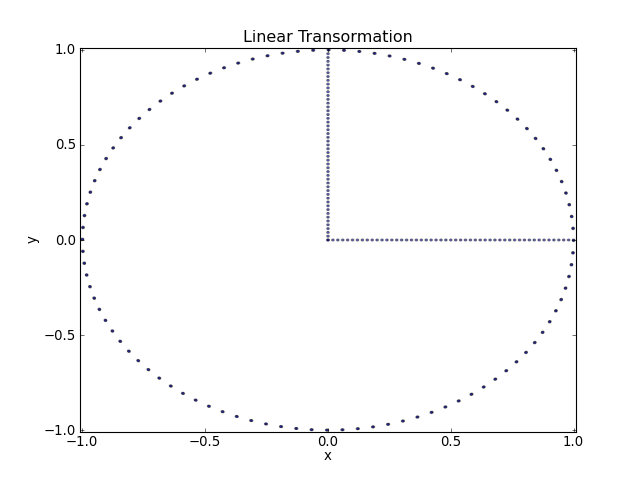
\includegraphics[width=1.5in]{images/la1.png} &
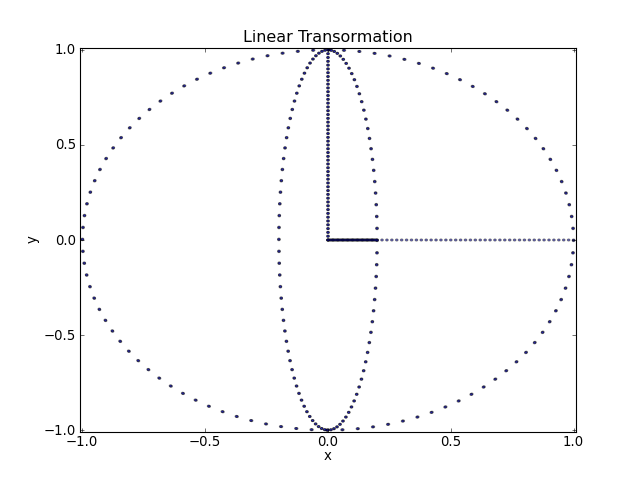
\includegraphics[width=1.5in]{images/la2.png} \\
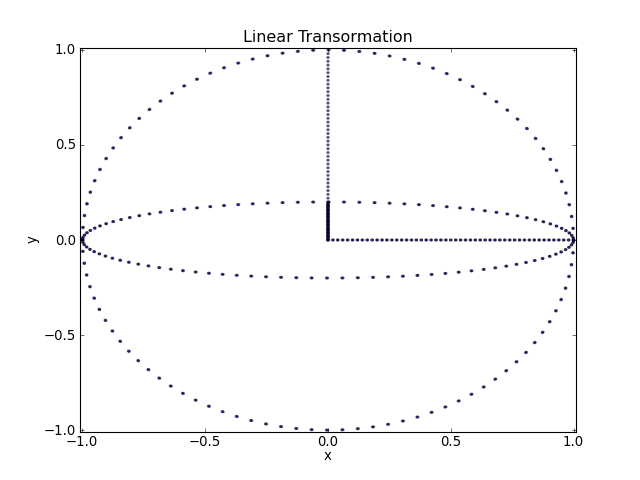
\includegraphics[width=1.5in]{images/la3.png} &
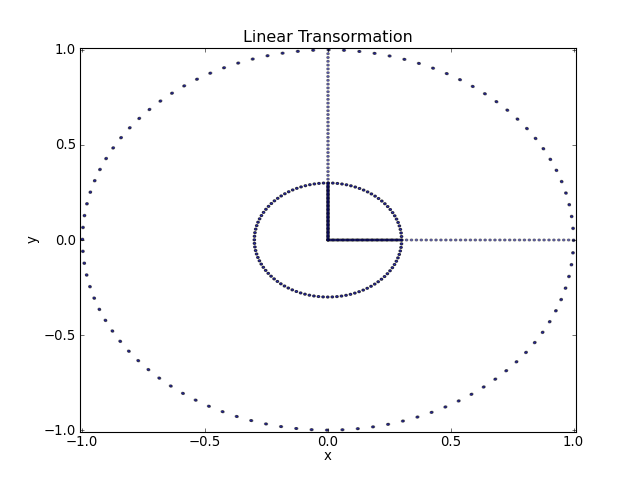
\includegraphics[width=1.5in]{images/la4.png} \\
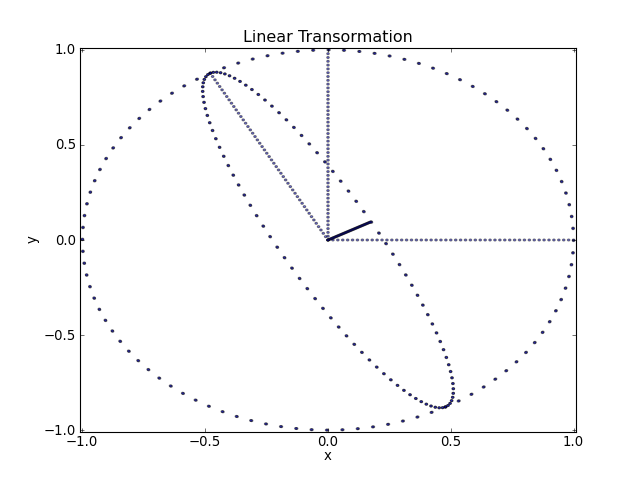
\includegraphics[width=1.5in]{images/la5.png} &
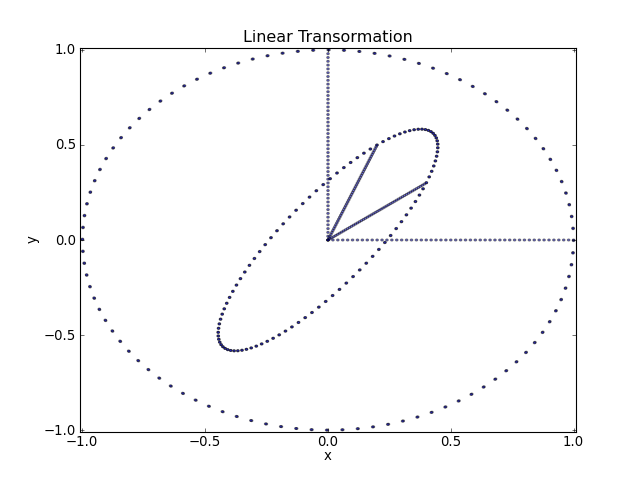
\includegraphics[width=1.5in]{images/la6.png}
\end{tabular}
\caption{Example of the effect of different linear transformations on the same set of points. From left to right, top to bottom, they show stretching along both the $X$- and $Y$-axes, scaling across both axes, a rotation, and a generic transformation that does not preserve angles.}
\end{figure}

\goodbreak\subsection{Matrix inversion and the Gauss--Jordan algorithm}

\index{matrix!inversion}\index{Gauss-Jordan}

Implementing the inverse of the multiplication (division) is a more challenging task.

We define $A^{-1}$, the inverse of the square matrix $A$, as that matrix such that for every vector $b$, $A\mathbf(x)=\mathbf{b}$ implies $\mathbf(x)=A^{-1}\mathbf{b}$. The Gauss--Jordan algorithm computes $A^{-1}$ given $A$.

To implement it, we must first understand how it works. Consider the following equation:

\begin{equation}
A \mathbf{x} = \mathbf{b}
\end{equation}
We can rewrite it as:
\begin{equation}
A \mathbf{x} = B \mathbf{b}
\end{equation}
where $B=1$, the identity matrix. This equation remains true if we multiply both terms by a nonsingular matrix $S_0$:
\begin{equation}
S_0 A \mathbf{x} = S_0 B \mathbf{b}
\end{equation}
The trick of the Gauss--Jordan elimination consists in finding a series of matrices $S_0$, $S_1$, ..., $S_{n-1}$ so that
\begin{equation}
S_{n-1} ... S_1 S_0 A \mathbf{x} = S_{n-1} ... S_1 S_0 B \mathbf{b} = \mathbf{x}
\end{equation}
Because the preceding expression must be true for every $b$ and because $x$ is the solution of $A x=b$, by definition, 
$S_{n-1} \ldots S_1 S_0 B \equiv A^{-1}$.

The Gauss-Jordan algorithm works exactly this way: given $A$, it computes $A^{-1}$:

%%% META:FILE:nlib/matrix.nim
\begin{lstlisting}[caption={in file: {\ft nlib/matrix.nim}}]
proc inv*(a0: Matrix, x = 1.0): Matrix =
  ## Returns x * a^-1 using Gauss-Jordan elimination.
  let n = a0.ncols
  if a0.nrows != n:
    raise newException(ArithmeticDefect, "matrix not squared")
  let a = newMatrix(a0.tolist())   # copy
  let b = identity(n, x)
  for c in 0 ..< n:
    for r in c + 1 ..< n:
      if abs(a[r, c]) > abs(a[c, c]):
        a.swapRows(r, c)
        b.swapRows(r, c)
    let p = a[c, c]
    for k in 0 ..< n:
      a[c, k] = a[c, k] / p
      b[c, k] = b[c, k] / p
    for r in 0 ..< n:
      if r == c: continue
      let pr = a[r, c]
      for k in 0 ..< n:
        a[r, k] = a[r, k] - a[c, k] * pr
        b[r, k] = b[r, k] - b[c, k] * pr
  result = b

proc `/`*(x: float, a: Matrix): Matrix = inv(a, x)
proc `/`*(a: Matrix, x: float): Matrix = (1.0 / x) * a
proc `/`*(a, b: Matrix): Matrix = a * (1.0 / b)
\end{lstlisting}

Here is an example, and we will see many more applications later:

\begin{lstlisting}
let A = newMatrix(@[@[1.0, 2.0], @[4.0, 9.0]])
echo 1.0 / A    # @[@[9.0, -2.0], @[-4.0, 1.0]]
echo A / A      # @[@[1.0, 0.0], @[0.0, 1.0]]
echo A / 2.0    # @[@[0.5, 1.0], @[2.0, 4.5]]
\end{lstlisting}

\goodbreak\subsection{Transposing a matrix}

\index{matrix!transpose}

Another operation that we will need is transposition:

%%% META:FILE:nlib/matrix.nim
\begin{lstlisting}[caption={in file: {\ft nlib/matrix.nim}}]
proc T*(a: Matrix): Matrix =
  ## Transpose of `a`.
  newMatrix(a.ncols, a.nrows,
    proc(r, c: int): float = a[c, r])
\end{lstlisting}

Notice the new matrix is defined with the number of rows and columns switched from matrix A. In Nim, a no-argument procedure can be called as either {\ft a.T()} or {\ft a.T} thanks to the uniform-call-syntax rule.
This can be used as follows:

\begin{lstlisting}
let A = newMatrix(@[@[1.0, 2.0], @[3.0, 4.0]])
echo A.T()      # @[@[1.0, 3.0], @[2.0, 4.0]]
\end{lstlisting}

For later use, we define two functions to check whether a matrix is symmetrical or zero within a given precision.

Another typical transformation for matrices of complex numbers is the Hermitian operation, which is a transposition combined with complex conjugation of the elements. Since our {\ft Matrix} type stores {\ft float} values, the Hermitian coincides with the transpose; for a complex {\ft Matrix[Complex]} the same template would apply {\ft conj} element-wise.

\index{matrix!symmetric}

In later algorithms we will need to check whether a matrix is symmetrical (or almost symmetrical given precision) or zero (or almost zero):

%%% META:FILE:nlib/matrix.nim
\begin{lstlisting}[caption={in file: {\ft nlib/matrix.nim}}]
proc isAlmostSymmetric*(a: Matrix, ap = 1e-6, rp = 1e-4): bool =
  if a.nrows != a.ncols: return false
  for r in 0 ..< a.nrows:
    for c in 0 ..< r:
      let delta = abs(a[r, c] - a[c, r])
      if delta > ap and delta > max(abs(a[r, c]), abs(a[c, r])) * rp:
        return false
  return true

proc isAlmostZero*(a: Matrix, ap = 1e-6, rp = 1e-4): bool =
  for r in 0 ..< a.nrows:
    for c in 0 ..< a.ncols:
      let delta = abs(a[r, c] - a[c, r])
      if delta > ap and delta > max(abs(a[r, c]), abs(a[c, r])) * rp:
        return false
  return true
\end{lstlisting}

\goodbreak\subsection{Solving systems of linear equations}

\index{linear equations}\index{systems}

Linear algebra is fundamental for solving systems of linear equations such as the following:

\begin{eqnarray}
&x_0+2x_1+2x_2=&3 \\
&4x_0+4x_1+2x_2=&6 \\
&4x_0+6x_1+4x_2=&10
\end{eqnarray}
This can be rewritten using the equivalent linear algebra notation:
\begin{equation}
A \textrm{x} = \textrm{b}
\end{equation}
where
\begin{equation}
A = \left(\begin{tabular}{ccc}
1 & 2 & 2 \\
4 & 4 & 2 \\
4 & 6 & 4 \\
\end{tabular}\right) \qquad and \qquad
b =
\left(\begin{tabular}{c}
3 \\
6 \\
10 \\
\end{tabular}\right)
\end{equation}

The solution of the equation can now be written as
\begin{equation}
\textrm{x} = A^{-1}\textrm{b}
\end{equation}

We can easily solve the system with our library:

\begin{lstlisting}
let A = newMatrix(@[@[1.0, 2.0, 2.0], @[4.0, 4.0, 2.0], @[4.0, 6.0, 4.0]])
let b = newMatrix(@[3.0, 6.0, 10.0])
let x = (1.0 / A) * b
echo x          # @[@[-1.0], @[3.0], @[-1.0]]
\end{lstlisting}

Notice that $b$ is a column vector and therefore

\begin{lstlisting}
let b = newMatrix(@[3.0, 6.0, 10.0])
\end{lstlisting}

but not

\begin{lstlisting}
let b = newMatrix(@[@[3.0, 6.0, 10.0]])  # wrong: row vector
\end{lstlisting}

We can also obtain a column vector by performing a transposition of a row vector:

\begin{lstlisting}
let b = newMatrix(@[@[3.0, 6.0, 10.0]]).T()
\end{lstlisting}

\goodbreak\subsection{Norm and condition number again}

\index{matrix!norm}\index{condition number}\index{matrix!condition number}

By norm of a vector, we often refer to the 2-norm defined using the Pythagoras theorem:
\begin{equation}
||x||_2 = \sqrt{\sum_i x_i^2}
\end{equation}

For a vector, we can define the $p$-norm as a generalization of the $2$-norm:

\begin{equation}
||x||_p \equiv \left(\sum_i abs(x_i)^p \right)^{\frac1p}
\end{equation}

We can extend the notation of a norm to any function that maps a vector into a vector, as follows:

\begin{equation}
||f||_p \equiv \textrm{max}_x ||f(x)||_p / ||x||_p
\end{equation}

An immediate application is to functions implemented as linear transformations:

\begin{equation}
||A||_p \equiv \textrm{max}_x ||Ax||_p / ||x||_p
\end{equation}

This can be difficult to compute in the general case, but it reduces to a simple formula for the 1-norm:

\begin{equation}
||A||_1 \equiv \textrm{max}_j \sum_i abs(A_{ij})
\end{equation}

The 2-norm is difficult to compute for a matrix, but the 1-norm provides an approximation. It is computed by adding up the magnitude of the elements per each column and finding the maximum sum.

This allows us to define a generic function to compute the norm of lists, matrices/vectors, and scalars:

%%% META:FILE:nlib/linalg.nim
\begin{lstlisting}[caption={in file: {\ft nlib/linalg.nim}}]
proc norm*(x: float, p = 1): float = abs(x)

proc norm*(xs: seq[float], p = 1): float =
  var s = 0.0
  for x in xs: s += abs(x).pow(float(p))
  result = s.pow(1.0 / float(p))

proc norm*(a: Matrix, p = 1): float =
  if a.nrows == 1 or a.ncols == 1:
    var s = 0.0
    for r in 0 ..< a.nrows:
      for c in 0 ..< a.ncols:
        s += abs(a[r, c]).pow(float(p))
    return s.pow(1.0 / float(p))
  if p == 1:
    var best = 0.0
    for c in 0 ..< a.ncols:
      var s = 0.0
      for r in 0 ..< a.nrows: s += abs(a[r, c])
      if s > best: best = s
    return best
  raise newException(ValueError, "norm not implemented for p != 1 on matrix")
\end{lstlisting}

Now we can implement a function that computes the condition number for ordinary functions as well as for linear transformations represented by a matrix:

%%% META:FILE:nlib/linalg.nim
\begin{lstlisting}[caption={in file: {\ft nlib/linalg.nim}}]
proc conditionNumber*(f: proc(x: float): float, x: float,
                      h = 1e-6): float =
  D(f, h)(x) * x / f(x)

proc conditionNumber*(a: Matrix): float =
  norm(a) * norm(1.0 / a)
\end{lstlisting}

Here are some examples:

\begin{lstlisting}
proc f(x: float): float = x * x - 5.0 * x
echo formatFloat(conditionNumber(f, 1.0), ffDecimal, 2)
# 0.75
let A = newMatrix(@[@[1.0, 2.0], @[3.0, 4.0]])
echo formatFloat(conditionNumber(A), ffDecimal, 2)
# 21.0
\end{lstlisting}

\index{matrix!exponential}

Having the norm for matrices also allows us to extend the definition of convergence of a Taylor series to a series of matrices:

%%% META:FILE:nlib/linalg.nim
\begin{lstlisting}[caption={in file: {\ft nlib/linalg.nim}}]
proc exp*(a: Matrix, ap = 1e-6, rp = 1e-4, ns = 40): Matrix =
  ## Matrix exponential by Taylor series.
  var t = identity(a.ncols)
  var s = identity(a.ncols)
  for k in 1 ..< ns:
    t = t * a * (1.0 / float(k))
    s = s + t
    if norm(t) < max(ap, norm(s) * rp):
      return s
  raise newException(ArithmeticDefect, "no convergence")
\end{lstlisting}

\begin{lstlisting}
let A = newMatrix(@[@[1.0, 2.0], @[3.0, 4.0]])
echo exp(A)
# @[@[51.96..., 74.73...], @[112.10..., 164.07...]]
\end{lstlisting}

\goodbreak\subsection{Cholesky factorization}

\index{Cholesky}\index{matrix!positive definite}\index{positive definite}

A matrix is said to be positive definite if $x^t Ax>0$ for every $x\neq0$.

If a matrix is symmetric and positive definite, then there exists a lower triangular matrix $L$ such that $A=L L^t$. A lower triangular matrix is a matrix that has zeros above the diagonal elements.

The Cholesky algorithm takes a matrix $A$ as input and returns the matrix $L$:

%%% META:FILE:nlib/linalg.nim
\begin{lstlisting}[caption={in file: {\ft nlib/linalg.nim}}]
proc cholesky*(a: Matrix): Matrix =
  ## Cholesky decomposition: returns lower-triangular `L`
  ## such that `L * L.T == a`.
  if not isAlmostSymmetric(a):
    raise newException(ArithmeticDefect, "not symmetric")
  let l = newMatrix(a.tolist())   # copy
  for k in 0 ..< l.ncols:
    if l[k, k] <= 0:
      raise newException(ArithmeticDefect, "not positive definite")
    let p = sqrt(l[k, k])
    l[k, k] = p
    for i in k + 1 ..< l.nrows:
      l[i, k] = l[i, k] / p
    for j in k + 1 ..< l.nrows:
      let pj = l[j, k]
      for i in k + 1 ..< l.nrows:
        l[i, j] = l[i, j] - pj * l[i, k]
  for i in 0 ..< l.nrows:
    for j in i + 1 ..< l.ncols:
      l[i, j] = 0
  result = l
\end{lstlisting}

Here we provide an example and a check that indeed $A=L L^t$:

\begin{lstlisting}
let A = newMatrix(@[@[4.0, 2.0, 1.0],
                    @[2.0, 9.0, 3.0],
                    @[1.0, 3.0, 16.0]])
let L = cholesky(A)
echo isAlmostZero(A - L * L.T())   # true
\end{lstlisting}

The Cholesky algorithm fails if and only if the input matrix is not symmetric or not positive definite, therefore it can be used to check whether a symmetric matrix is positive definite.

Consider for example a generic covariance matrix $A$. It is supposed to be positive definite, but sometimes it is not, because it is computed incorrectly by taking different subsets of the data to compute $A_{ij}$, $A_{jk}$, and $A_{ik}$. The Cholesky algorithm provides an algorithm to check whether a matrix is positive definite:

%%% META:FILE:nlib/linalg.nim
\begin{lstlisting}[caption={in file: {\ft nlib/linalg.nim}}]
proc isPositiveDefinite*(a: Matrix): bool =
  if not isAlmostSymmetric(a):
    return false
  try:
    discard cholesky(a)
    return true
  except Defect:        # cholesky raises ArithmeticDefect on indefinites
    return false
  except CatchableError:
    return false
\end{lstlisting}

Another application of the Cholesky is in generating vectors $\mathbf{x}$ with probability distribution

\begin{equation}
p(\mathbf{x}) \propto \exp\left(-\frac12 \mathbf{x}^t A^{-1} \mathbf{x}\right)
\end{equation}
where $A$ is a symmetric and positive definite matrix. In fact, if $A=LL^t$, then
\begin{equation}
p(\mathbf{x}) \propto \exp\left(-\frac12 (L^{-1}\mathbf{x})^t (L^{-1}\mathbf{x})\right)
\end{equation}
and with a change of variable $\mathbf{u}=\mathbf{L^{-1}x}$, we obtain
\begin{equation}
p(\mathbf{x}) \propto \exp\left(-\frac12 \mathbf{u}^t \mathbf{u}\right)
\end{equation}
and
\begin{equation}
p(\mathbf{x}) \propto e^{-\frac12 u_0^2}e^{-\frac12 u_1^2}e^{-\frac12 u_2^2}...
\end{equation}
Therefore the $u_i$ components are Gaussian random variables.

In summary, given a covariance matrix $A$, we can generate random vectors $x$ or random numbers with the same covariance simply by doing

%%% META:FILE:nlib/finance.nim
\begin{lstlisting}[caption={in file: {\ft nlib/finance.nim}}]
iterator randomList*(a: Matrix): seq[float] =
  ## Yields successive random vectors with covariance matrix `a`.
  let l = cholesky(a)
  while true:
    var u = newMatrix(l.nrows, 1)
    for c in 0 ..< l.nrows: u[c, 0] = gauss(0.0, 1.0)
    yield (l * u).flatten()
\end{lstlisting}

Here is an example of how to use it:

\begin{lstlisting}
let A = newMatrix(@[@[1.0, 0.1], @[0.2, 3.0]])
for v in randomList(A):
  echo v
\end{lstlisting}

The {\ft RandomList} is a generator. You can iterate over it. The {\ft yield} keyword is used like {\ft return}, except the function will return a generator.

\goodbreak\subsection{Modern portfolio theory}

\index{Modern Portfolio Theory}\index{tangency portfolio}\index{Markowitz}\index{Sharpe ratio}

Modern portfolio theory~\cite{mpt} is an investment approach that tries to maximize return given a fixed risk. Many different metrics have been proposed. One of them is the {\it Sharpe ratio}.

For a stock or a portfolio with an average return $r$ and risk $\sigma$, the Sharpe ratio is defined as
\begin{equation}
\textrm{Sharpe}(r, \sigma) \equiv (r-\bar r)/\sigma
\end{equation}
Here $\bar r$ is the current risk-free investment rate. Usually the risk is measured as the standard deviation of its daily (or monthly or yearly) return.

Consider the stock price $p_{it}$ of stock $i$ at time $t$ and its arithmetic daily return
$r_{it}=(p_{i, t+1}-p_{it})/p_{it}$ given a risk-free interest equal to $\bar r$.

For each stock, we can compute the average return and average risk (variance of daily returns) and display it in a risk-return plot as we did in chapter 2.

We can try to build arbitrary portfolios by investing in multiple stocks at the same time. Modern portfolio theory states that there is a maximum Sharpe ratio and there is one portfolio that corresponds to it. It is called the tangency portfolio.

A portfolio is identified by fractions of \$1 invested in each stock in the portfolio. Our goal is to determine the tangent portfolio.

If we assume that daily returns for the stocks are Gaussian, then the solving algorithm is simple.

All we need is to compute the average return for each stock, defined as
\begin{equation}
r_i = 1/T \sum_t r_{it}
\end{equation}
and the covariance matrix
\begin{equation}
A_{ij} = \frac1T \sum_t (r_{it}-r_i)(r_{jt}-r_j)
\end{equation}

Modern portfolio theory tells us that the tangent portfolio is given by
\begin{equation}
\mathbf{x}=A^{-1} ( \mathbf{r}-\bar{r}\mathbf{1})
\end{equation}

The inputs of the formula are the covariance matrix ($A$), a vector or arithmetic returns for the assets in the portfolio ($r$), the risk free rate ($\bar{r}$). The output is a vector ($x$) whose elements are the percentages to be invested in each asset to obtain a tangency portfolio. Notice that some elements of $x$ can be negative and this corresponds to short position (sell, not buy, the asset).

Here is the algorithm:

%%% META:FILE:nlib/finance.nim
\begin{lstlisting}[caption={in file: {\ft nlib/finance.nim}}]
proc markowitz*(mu, a: Matrix, rFree: float):
                (seq[float], float, float) =
  ## Markowitz tangency portfolio. Returns (weights, return, risk).
  var x = (1.0 / a) * (mu - rFree)
  var s = 0.0
  for r in 0 ..< x.nrows: s += x[r, 0]
  x = x / s
  var portfolio: seq[float] = @[]
  for r in 0 ..< x.nrows: portfolio.add x[r, 0]
  let ret = (mu.T * x)[0, 0]
  let risk = sqrt((x.T * (a * x))[0, 0])
  (portfolio, ret, risk)
\end{lstlisting}

Here is an example.
We consider three assets (0, 1, 2) with the following covariance matrix:
\begin{lstlisting}
let cov = newMatrix(@[@[0.04, 0.006, 0.02],
                      @[0.006, 0.09, 0.06],
                      @[0.02, 0.06, 0.16]])
\end{lstlisting}
and the following expected returns (arithmetic returns, not log returns, because the former are additive, whereas the latter are not):
\begin{lstlisting}
let mu = newMatrix(@[0.10, 0.12, 0.15])
\end{lstlisting}
Given the risk-free interest rate
\begin{lstlisting}
let rFree = 0.05
\end{lstlisting}
we compute the tangent portfolio (highest Sharpe ratio), its return, and its risk with one function call:
\begin{lstlisting}
let (x, ret, risk) = markowitz(mu, cov, rFree)
echo x
# @[0.5566343042071198, 0.27508090614886727, 0.16828478964401297]
echo ret, " ", risk
# 0.113915857605 0.186747095412
echo (ret - rFree) / risk
# 0.34225891152
for r in 0 ..< 3:
  echo (mu[r, 0] - rFree) / sqrt(cov[r, r])
# 0.25
# 0.233333333333
# 0.25
\end{lstlisting}

Investing 55\% in asset 0, 27\% in asset 1, and 16\% in asset 2, the resulting portfolio has an expected return of 11.39\% and a risk of 18.67\%, which corresponds to a Sharpe ratio of 0.34, much higher than 0.25, 0.23, and 0.23 for the individual assets.

Notice that the tangency portfolio is not the only one with the highest Sharpe ratio (return for unit of risk). In fact, any linear combination of the tangency portfolio with a risk-free asset (putting money in the bank) has the same Sharpe ratio. For any target risk, one can find a linear combination of the risk-free asset and the tangent portfolio that has a better Sharpe ratio than any other possible portfolio comprising the same assets.

If we call $\alpha$ the fraction of the money to invest in the tangency portfolio and $1-\alpha$ the fraction to keep in the bank at the risk free rate, the resulting combined portfolio has return:

\begin{equation}
\alpha \mathbf{x}\cdot\mathbf{r} + (1-\alpha) \bar r
\end{equation}

and risk

\begin{equation}
\alpha \sqrt{\mathbf{x}^t A \mathbf{x}}
\end{equation}

We can determine $\alpha$ by deciding how much risk we are willing to take, and these formulas tell us the optimal portfolio for that amount of risk.


\goodbreak\subsection{Linear least squares, $\chi^2$}

\index{linear least squares}\index{$\chi^2$}\index{fitting}\index{Regression}

Consider a set of data points $(x_J, y_j) = (t_j, o_j \pm do_j)$. We want to fit them with a linear combination of linear independent functions $f_i$ so that

\begin{eqnarray}
c_0 f_0(t_0) + c_1 f_1(t_0) + c_2 f_2(t_0) +  ... & = & e_0 \simeq o_0 \pm do_0\\
c_0 f_0(t_1) + c_1 f_1(t_1) + c_2 f_2(t_1) +  ... & = & e_1 \simeq o_1 \pm do_1\\
c_0 f_0(t_2) + c_1 f_1(t_2) + c_2 f_2(t_2) +  ... & = & e_2 \simeq o_2 \pm do_2\\
... &=& ...
\end{eqnarray}

We want to find the $\{c_i\}$ that minimizes the sum of the squared distances between the actual ``observed'' data $o_j$ and the predicted ``expected'' data $e_j$, in units of $do_j$. This metric is called $\chi^2$ in general~\cite{chi2}. An algorithm that minimizes the $\chi^2$  and is linear in the $c_i$ coefficients (our case here) is called {\it linear least squares} or {\it linear regression}.

\begin{equation}
\chi^2 = \sum_j \left|\frac{e_j - o_j}{do_j}\right|^2
\end{equation}

If we define the matrix $A$ and $B$ as

\begin{equation}
A=\left(
\begin{tabular}{cccc}
$\frac{f_0(t_0)}{do_0}$ & $\frac{f_1(t_0)}{do_0}$ & $\frac{f_2(t_0)}{do_0}$ &...\\
$\frac{f_0(t_1)}{do_1}$ & $\frac{f_1(t_1)}{do_1}$ & $\frac{f_2(t_1)}{do_1}$ &...\\
$\frac{f_0(t_2)}{do_2}$ & $\frac{f_1(t_2)}{do_2}$ & $\frac{f_2(t_2)}{do_2}$ &...\\
...& ...& ... & ...
\end{tabular}
\right) \qquad b =
\left(
\begin{tabular}{c}
$\frac{o_0}{do_0}$ \\
$\frac{o_1}{do_1}$ \\
$\frac{o_2}{do_2}$ \\
...
\end{tabular}
\right)
\end{equation}

then the problem is reduced to

\begin{eqnarray}
\min_{\mathbf{c}}\chi^2 &=& \min_{\mathbf{c}} |A\mathbf{c}-\mathbf{b}|^2 \\
  &=& \min_{\mathbf{c}} (A\mathbf{c}-\mathbf{b})^t (A\mathbf{c}-\mathbf{b}) \\
  &=& \min_{\mathbf{c}} (\mathbf{c}^t A^t A \mathbf x - 2\mathbf{b}^t A \mathbf{c} + \mathbf{b}^t \mathbf{b})
\end{eqnarray}
This is the same as solving the following equation:

\begin{eqnarray}
\nabla_{c} (\mathbf{c}^t A^t A \mathbf x - 2\mathbf{c}^t A^t \mathbf{b} + \mathbf{b}^t\mathbf{b}) &=& 0 \\
A^t A \mathbf{c} - A^t \mathbf{b} &=& 0
\end{eqnarray}

Its solution is

\begin{equation}
\mathbf{c} = (A^t A)^{-1} (A^t \mathbf{b})
\end{equation}

The following algorithm implements a fitting function based on the preceding procedure. It takes as input a list of functions $f_i$ and a list of points $p_j=(t_j, o_j, do_j)$ and returns three objects---a list with the $c$ coefficients, the value of $\chi^2$ for the best fit, and the fitting function:

%%% META:FILE:nlib/fitting.nim
\begin{lstlisting}[caption={in file: {\ft nlib/fitting.nim}}]
type
  FitFunc* = proc(x: float): float

proc fitLeastSquares*(points: seq[(float, float, float)],
                      f: seq[FitFunc]):
                      (seq[float], float, proc(x: float): float) =
  ## Linear least-squares fit of `points = (x, y, dy)` to
  ## `\sum_j c_j f[j](x)`. Returns (coefficients, chi2, fit function).
  let n = points.len
  let m = f.len
  let a = newMatrix(n, m)
  let b = newMatrix(n, 1)
  for i in 0 ..< n:
    let weight = 1.0 / points[i][2]
    b[i, 0] = weight * points[i][1]
    for j in 0 ..< m:
      a[i, j] = weight * f[j](points[i][0])
  let c = (1.0 / (a.T * a)) * (a.T * b)
  let chi = a * c - b
  let chi2Val = norm(chi, 2) ^ 2
  let cs = c.flatten()
  let fittingF = proc(x: float): float =
    var s = 0.0
    for i in 0 ..< f.len: s += f[i](x) * cs[i]
    s
  (cs, chi2Val, fittingF)

# examples of fitting functions
proc polynomial*(n: int): seq[FitFunc] =
  proc monomial(power: int): FitFunc =
    # Wrap closure creation in a separate proc so each closure
    # captures its own `power` parameter (rather than sharing a
    # single mutable loop variable).
    result = proc(x: float): float = x ^ power
  for p in 0 .. n:
    result.add monomial(p)

let CONSTANT*  = polynomial(0)
let LINEAR*    = polynomial(1)
let QUADRATIC* = polynomial(2)
let CUBIC*     = polynomial(3)
let QUARTIC*   = polynomial(4)
\end{lstlisting}

As an example, we can use it to perform a polynomial fit: given a set of points, we want to find the coefficients of a polynomial that best approximate those points.

In other words, we want to find the $c_i$ such that, given $t_j$ and $o_j$, 
\begin{eqnarray}
c_0  + c_1 t_0^{1} + c_2 t_0^{2} +  ... & = & e_0 \simeq o_0 \pm do_0 \\
c_0  + c_1 t_1^{1} + c_2 t_1^{2} +  ... & = & e_1 \simeq o_1 \pm do_1\\
c_0  + c_1 t_2^{1} + c_2 t_2^{2} +  ... & = & e_2 \simeq o_2 \pm do_2\\
... &  &... \\
\end{eqnarray}

Here is how we can generate some random points and solve the problem for a polynomial of degree 2 (or quadratic fit):

\begin{lstlisting}
var points: seq[(float, float, float)] = @[]
for k in 0 ..< 100:
  let kf = float(k)
  points.add (kf, 5.0 + 0.8 * kf + 0.3 * kf * kf + sin(kf), 2.0)
let (a, chi2, fittingF) = fitLeastSquares(points, QUADRATIC)
for p in points[^10 .. ^1]:
  echo p[0], " ",
       formatFloat(p[1], ffDecimal, 2), " ",
       formatFloat(fittingF(p[0]), ffDecimal, 2)
# 90 2507.89 2506.98
# ...

# Render the first 10 observations with their error bars and the
# fitted polynomial through them.
savePlot("images/polynomialfit.png",
         points[0 ..< 10].mapIt(it[0]),
         points[0 ..< 10].mapIt(fittingF(it[0])),
         title = "polynomial fit", xlab = "t", ylab = "e(t), o(t)")
\end{lstlisting}

Fig.~\ref{fit} is a plot of the first 10 points compared with the best fit:

\begin{figure}[ht]
\centering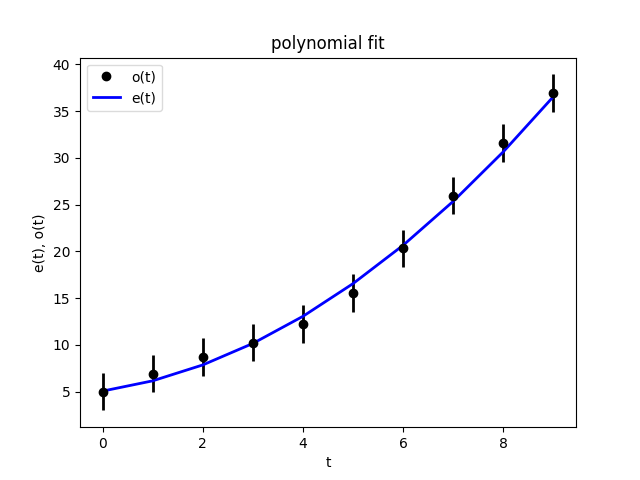
\includegraphics[width=4in]{images/polynomialfit.png}
\caption{Random data with their error bars and the polynomial best fit.\label{fit}}
\end{figure}

We can also define a $\chi^2_{dof} = \chi^2/(N-1)$ where $N$ is the number of $c$ parameters determined by the fit. A value of $\chi^2_{dof} \simeq 1$ indicates a good fit. In general, the smaller $\chi^2_{dof}$, the better the fit. A large value of $\chi^2_{dof}$ is a symptom of poor modeling (the assumptions of the fit are wrong), whereas a value $\chi^2_{dof}$ much smaller than 1 is a symptom of an overestimate of the errors $do_j$ (or perhaps manufactured data).

\goodbreak\subsection{Trading and technical analysis}

\index{trading strategy}\index{technical analysis}

In finance, {\it technical analysis} is an empirical discipline that consists of forecasting the direction of prices through the study of patterns in historical data (in particular, price and volume). As an example, we implement a simple strategy that consists of the following steps:

\begin{itemize}
\item We fit the adjusted closing price for the previous seven days and use our fitting function to predict the adjusted close for the next day.
\item If we have cash and predict the price will go up, we buy the stock.
\item If we hold the stock and predict the price will go down, we sell the stock.
\end{itemize}

\index{class!Trader}

%%% META:FILE:nlib/finance.nim
\begin{lstlisting}[caption={in file: {\ft nlib/finance.nim}}]
type
  Trader* = ref object

proc model*(t: Trader, window: seq[float]): float =
  ## Fit the last few days quadratically and extrapolate tomorrow's price.
  var points: seq[(float, float, float)] = @[]
  for i, v in window:
    points.add (float(i), v, 1.0)
  let (_, _, fittingF) = fitLeastSquares(points, QUADRATIC)
  fittingF(float(points.len))

proc strategy*(t: Trader, history: seq[float], ndays = 7): string =
  if history.len < ndays: return ""
  let todayClose = history[^1]
  let tomorrowPrediction = t.model(history[^ndays .. ^1])
  if tomorrowPrediction > todayClose: "buy" else: "sell"

proc simulate*(t: Trader, data: seq[float],
               cash = 1000.0, shares = 0.0,
               dailyRate = 0.03 / 360.0): float =
  var cash = cash
  var shares = shares
  for tIdx in 0 ..< data.len:
    let suggestion = t.strategy(data[0 ..< tIdx])
    let todayClose = data[max(tIdx - 1, 0)]
    if cash > 0 and suggestion == "buy":
      let sharesBought = float(int(cash / todayClose))
      shares += sharesBought
      cash -= sharesBought * todayClose
    elif shares > 0 and suggestion == "sell":
      cash += shares * todayClose
      shares = 0.0
    cash *= exp(dailyRate)
  cash + shares * data[^1]
\end{lstlisting}

Now we back test the strategy using fake financial data. We can generate fake financial data with this function:

%%% META:FILE:nlib/finance.nim
\begin{lstlisting}[caption={in file: {\ft nlib/finance.nim}}]
proc fakeStockPrices*(startPrice = 100.0, averageReturn = 0.05,
                     volatility = 0.30, days = 100): seq[float] =
  let dailyVolatility = volatility / sqrt(250.0)
  let dailyReturn = averageReturn / 250.0
  var s: seq[float] = @[]
  for _ in 0 ..< days - 1: s.add gauss(0.0, dailyVolatility)
  var sumS = 0.0
  for v in s: sumS += v
  let mu = dailyReturn - sumS / float(days - 1)
  var v = @[startPrice]
  for item in s:
    v.add v[^1] * exp(mu + item)
  result = v
\end{lstlisting}

\begin{lstlisting}
let initialCash = 1000.0
let data = fakeStockPrices(averageReturn = 0.05)
let finalCash = Trader().simulate(data, cash = initialCash)
let naiveProfit = initialCash * (exp(0.05) - 1.0)
let strategyProfit = finalCash - initialCash
\end{lstlisting}

If {\ft strategy\_profit} > {\ft naive\_profit} then our strategy outperforms the naive buy and hold strategy.

Of course, we can always engineer a strategy based on historical data that will outperform holding the stock, but {\it past performance is never a guarantee of future performance}.

According to the definition from investopedia.com, ``technical analysts believe that the historical performance of stocks and markets is an indication of future performance.''

The efficacy of both technical and fundamental analysis is disputed by the efficient-market hypothesis, which states that stock market prices are essentially unpredictable~\cite{andrew}.

It is easy to extend the previous class to implement other strategies and back test them.

\goodbreak\subsection{Eigenvalues and the Jacobi algorithm}

\index{eigenvalues}\index{eigenvectors}\index{Jacobi}

Given a matrix $A$, an eigenvector is defined as a vector $\mathbf{x}$ such that
$A\mathbf{x}$ is proportional to $\mathbf{x}$.
The proportionality factor is called an eigenvalue, $e$. One matrix may have many eigenvectors $\mathbf{x}_i$ and associated eigenvalues $e_i$:

\begin{equation}
A\mathbf{x}_i = e_i\mathbf{x}_i
\end{equation}

For example:
\begin{equation}
A = \left(\begin{tabular}{ccc}
1 & -2  \\
1 & 4  \\
\end{tabular}\right) \qquad and \qquad
x_i =
\left(\begin{tabular}{c}
-1 \\
1 \\
\end{tabular}\right)
\end{equation}

\begin{equation}
\left(\begin{tabular}{ccc}
1 & -2  \\
1 & 4  \\
\end{tabular}\right) * 
\left(\begin{tabular}{c}
-1 \\
1 \\
\end{tabular}\right) \qquad =  \qquad
3 * \left(\begin{tabular}{c}
-1 \\
1 \\
\end{tabular}\right)
\end{equation}

In this case, $x_i$ is an eigenvector and the corresponding eigenvalue is $e=3$.

Some eigenvalues may be zero ($e_i=0$), which means the matrix $A$ is singular. A matrix is singular if it maps a nonzero vector into zero.

Given a square matrix $A$, if the space generated by the linear independent eigenvalues has the same dimensionality as the number of rows (or columns) of $A$, then its eigenvalues are real and the matrix can we written as

\begin{equation}
A = U D U^t
\end{equation}
where
$D$ is a diagonal matrix with eigenvalues on the diagonal $D_{ii} = e_i$ and
$U$ is a matrix whose column $i$ is the $\mathbf{x}_i$ eigenvalue.

The following algorithm is called the Jacobi algorithm. It takes as input a symmetric matrix $A$ and returns the matrix $U$ and a list of corresponding eigenvalues $e$, sorted from smallest to largest:


%%% META:FILE:nlib/linalg.nim
\begin{lstlisting}[caption={in file: {\ft nlib/linalg.nim}}]
proc jacobiEigenvalues*(a: Matrix): (Matrix, seq[float]) =
  ## Returns (U, e) so that `a == U * diagonal(e) * U.T`.
  ## The i-th column of U is the eigenvector for eigenvalue `e[i]`.
  proc maxind(m: Matrix, k: int): int =
    var j = k + 1
    for i in k + 2 ..< m.ncols:
      if abs(m[k, i]) > abs(m[k, j]): j = i
    j
  let n = a.nrows
  if n != a.ncols:
    raise newException(ArithmeticDefect, "matrix not squared")
  let s = newMatrix(a.tolist())
  let eMat = identity(n)
  var state = n
  var ind = newSeq[int](n)
  var e = newSeq[float](n)
  var changed = newSeq[bool](n)
  for k in 0 ..< n:
    ind[k] = maxind(s, k)
    e[k] = s[k, k]
    changed[k] = true
  while state > 0:
    var m = 0
    for k in 1 ..< n - 1:
      if abs(s[k, ind[k]]) > abs(s[m, ind[m]]): m = k
    let k = m
    let h = ind[m]
    let p = s[k, h]
    var y = (e[h] - e[k]) / 2.0
    var t = abs(y) + sqrt(p * p + y * y)
    var sv = sqrt(p * p + t * t)
    var c = t / sv
    var ss = p / sv
    t = p * p / t
    if y < 0:
      ss = -ss
      t = -t
    s[k, h] = 0
    y = e[k]
    e[k] = y - t
    if changed[k] and y == e[k]:
      changed[k] = false; dec state
    elif (not changed[k]) and y != e[k]:
      changed[k] = true; inc state
    y = e[h]
    e[h] = y + t
    if changed[h] and y == e[h]:
      changed[h] = false; dec state
    elif (not changed[h]) and y != e[h]:
      changed[h] = true; inc state
    for i in 0 ..< k:
      let a1 = c * s[i, k] - ss * s[i, h]
      let a2 = ss * s[i, k] + c * s[i, h]
      s[i, k] = a1; s[i, h] = a2
    for i in k + 1 ..< h:
      let a1 = c * s[k, i] - ss * s[i, h]
      let a2 = ss * s[k, i] + c * s[i, h]
      s[k, i] = a1; s[i, h] = a2
    for i in h + 1 ..< n:
      let a1 = c * s[k, i] - ss * s[h, i]
      let a2 = ss * s[k, i] + c * s[h, i]
      s[k, i] = a1; s[h, i] = a2
    for i in 0 ..< n:
      let a1 = c * eMat[k, i] - ss * eMat[h, i]
      let a2 = ss * eMat[k, i] + c * eMat[h, i]
      eMat[k, i] = a1; eMat[h, i] = a2
    ind[k] = maxind(s, k)
    ind[h] = maxind(s, h)
  # sort vectors
  for i in 1 ..< n:
    var j = i
    while j > 0 and e[j - 1] > e[j]:
      swap(e[j], e[j - 1])
      eMat.swapRows(j, j - 1)
      dec j
  # normalize vectors
  let u = newMatrix(n, n)
  for i in 0 ..< n:
    var s2 = 0.0
    for j in 0 ..< n: s2 += eMat[i, j] ^ 2
    let nrm = sqrt(s2)
    for j in 0 ..< n: u[j, i] = eMat[i, j] / nrm
  (u, e)
\end{lstlisting}

Here is an example that shows, for a particular case, the relation between the input, $A$, of the output of the $U, e$ of the Jacobi algorithm:

\begin{lstlisting}
randomize()
let A = newMatrix(4, 4)
for r in 0 ..< A.nrows:
  for c in r ..< A.ncols:
    A[r, c] = gauss(10.0, 10.0)
    A[c, r] = A[r, c]
let (U, e) = jacobiEigenvalues(A)
echo isAlmostZero(U * diagonal(e) * U.T() - A)   # true
\end{lstlisting}

Eigenvalues can be used to filter noise out of data and find hidden dependencies in data. Following are some examples.

\goodbreak\subsection{Principal component analysis}

\index{principal component analysis}\index{correlation}

One important application of the Jacobi algorithm is for principal component analysis (PCA). This is a mathematical procedure that converts a set of observations of possibly correlated vectors into a set of uncorrelated vectors called {\it principal components}.

Here we consider, as an example, the time series of the adjusted arithmetic returns for the S\&P100 stocks that we downloaded and stored in chapter 2.

Each time series is a vector. We know they are not independent because there are correlations. Our goal is to model each time series and a vector plus noise where the vector is the same for all series. We also want find that vector that has maximal superposition with the individual time series, the principal component.

First, we compute the correlation matrix for all the stocks. This is a nontrivial task because we have to make sure that we only consider those days when all stocks were traded. %%%% FIXME EXPLAIN MORE

%%%% FIXME EXAMPLE?

%%% META:FILE:nlib/linalg.nim
\begin{lstlisting}[caption={in file: {\ft nlib/linalg.nim}}]
proc computeCorrelationMatrix*(v: seq[seq[float]]): Matrix =
  ## Pearson correlation matrix of `v` (rows are series).
  let m = v.len
  let n = v[0].len
  var mus = newSeq[float](m)
  var vars = newSeq[float](m)
  for i in 0 ..< m:
    var s = 0.0
    for k in 0 ..< n: s += v[i][k]
    mus[i] = s / float(n)
    var s2 = 0.0
    for k in 0 ..< n: s2 += v[i][k] ^ 2
    vars[i] = s2 / float(n) - mus[i] ^ 2
  result = newMatrix(m, m,
    proc(i, j: int): float =
      var s = 0.0
      for k in 1 ..< n: s += v[i][k] * v[j][k]
      (s / float(n) - mus[i] * mus[j]) / sqrt(vars[i] * vars[j]))
\end{lstlisting}

We use the preceding function to compute the correlation and pass it as input to the Jacobi algorithm and plot the output eigenvalues:

\begin{lstlisting}
var stocks: seq[seq[float]] = @[]
for _ in 0 ..< 5: stocks.add fakeStockPrices()
let corr = computeCorrelationMatrix(stocks)
let (U, e) = jacobiEigenvalues(corr)
savePlot("images/correlations.png",
         (0 ..< e.len).toSeq().mapIt(float(it)),
         e, title = "Fake Stock Correlations",
         xlab = "i", ylab = "e[i]")
\end{lstlisting}

\begin{figure}[ht]
\centering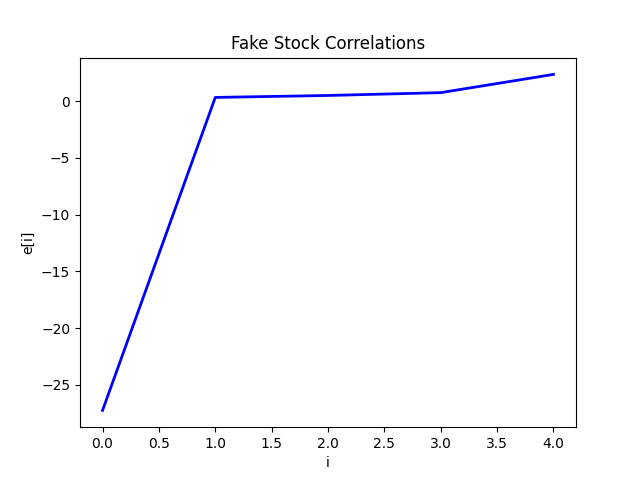
\includegraphics[width=4in]{images/correlations.png}
\caption{Eigenvalues of the correlation matrix for 5 fake stocks stocks, sorted by their magnitude.}
\end{figure}

\index{alpha}\index{beta}

The image shows that one eigenvalue, the last one, is much larger than the others. It tells us that the data series have something in common. In fact, the arithmetic returns for stock $j$ at time $t$ can be written as

\begin{equation}
r_{it} = \beta_i p_t + \alpha_{it}
\end{equation}
where $p$ is the principal component given by

\begin{eqnarray}
p_t &=& \sum_i U_{n-1, j} r_{jt} \\
\beta_i &=& \sum_t r_{it} p_t \\
\alpha_{it} &=& r_{it} - \beta_i p_t
\end{eqnarray}

Here $\mathbf{p}$ is the vector of adjusted arithmetic returns that better correlates with the returns of the individual assets and therefore best represents the market. The $\beta_i$ coefficient tells us how much $\mathbf{r}_i$ overlaps with $\mathbf{p}$; $\alpha$, at first approximation, measures leftover noise.

\goodbreak\section{Sparse matrix inversion}

\index{sparse matrix}

Sometimes we have to invert matrices that are very large, and the Gauss-Jordan algorithm fails. Yet, if the matrix is sparse, in the sense that most of its elements are zeros, then two algorithms come to our rescue: the {\it minimum residual} and the {\it biconjugate gradient} (for which we consider a variant called the {\it stabilized bi-conjugate gradient}).

We will also assume that the matrix to be inverted is given in some implicit algorithmic as $\mathbf{y}=f(\mathbf{x})$ because this is always the case for sparse matrices. There is no point to storing all its elements because most of them are zero.

%%%% FIXME CODE

\goodbreak\subsection{Minimum residual}

\index{minimum residual}

Given a linear operator $f$, the Krylov space spanned by a vector $x$ is defined as

\begin{equation}
K(f, y, i) = \{y, f(y), f(f(y)), f(f(f(y))), (f^i)(y)\}
\end{equation}
The {\it minimum residual}~\cite{minres} algorithm works by solving $x=f^{-1}(y)$ iteratively. At each iteration, it computes a new orthogonal basis vector $q_i$ for the Krylov space $K(f, y, i)$ and computes the coefficients $\alpha_i$ that project $x_i$ into component $i$ of the Krylov space:
\begin{equation}
x_i = y + \alpha_1 q_1 + \alpha_2 q_2 + ... + \alpha_i q_i \in K(f, y, i+1)
\end{equation}
which minimizes the norm of the residue defined as:
\begin{equation}
r = f(x_i) - y
\end{equation}
Therefore $\lim_{i\rightarrow\infty} f(x_i) = y$.
If a solution to the original problem exists, ignoring precision issues, the minimum residual converges to it, and the residue decreases at each iteration.

Notice that in the following code, $x$ and $y$ are exchanged because we adopt the convention that $y$ is the output and $x$ is the input:

%%% META:FILE:nlib/linalg.nim
\begin{lstlisting}[caption={in file: {\ft nlib/linalg.nim}}]
proc invertMinimumResidual*(f: proc(x: Matrix): Matrix,
                            x: Matrix,
                            ap = 1e-4, rp = 1e-4, ns = 200): Matrix =
  ## Minimum residual iterative solver for `f(x) = y` (sparse linear ops).
  var y = newMatrix(x.tolist())
  var r = x - f(x)
  for k in 0 ..< ns:
    let q = f(r)
    let alpha = (q.T * r)[0, 0] / (q.T * q)[0, 0]
    y = y + alpha * r
    r = r - alpha * q
    let residue = sqrt((r.T * r)[0, 0] / float(r.nrows))
    if residue < max(ap, norm(y) * rp): return y
  raise newException(ArithmeticDefect, "no convergence")
\end{lstlisting}

\goodbreak\subsection{Stabilized biconjugate gradient}

\index{bi-conjugate gradient}

The stabilized biconjugate gradient~\cite{bicgstab} method is also based on constructing a Krylov subspace and minimizing the same residue as in the minimum residual algorithm, yet it is faster than the minimum residual and has a smoother convergence than other conjugate gradient methods:

%%% META:FILE:nlib/linalg.nim
\begin{lstlisting}[caption={in file: {\ft nlib/linalg.nim}}]
proc invertBicgstab*(f: proc(x: Matrix): Matrix,
                     x: Matrix,
                     ap = 1e-4, rp = 1e-4, ns = 200): Matrix =
  ## Stabilized bi-conjugate gradient iterative solver.
  var y = newMatrix(x.tolist())
  var r = x - f(x)
  let q = newMatrix(r.tolist())
  var p = newMatrix(r.nrows, 1)
  var s = newMatrix(r.nrows, 1)
  var rhoOld = 1.0
  var alpha = 1.0
  var omega = 1.0
  for k in 0 ..< ns:
    let rho = (q.T * r)[0, 0]
    let beta = (rho / rhoOld) * (alpha / omega)
    rhoOld = rho
    p = beta * p + r - (beta * omega) * s
    s = f(p)
    alpha = rho / (q.T * s)[0, 0]
    r = r - alpha * s
    let tt = f(r)
    omega = (tt.T * r)[0, 0] / (tt.T * tt)[0, 0]
    y = y + omega * r + alpha * p
    let residue = sqrt((r.T * r)[0, 0] / float(r.nrows))
    if residue < max(ap, norm(y) * rp): return y
    r = r - omega * tt
  raise newException(ArithmeticDefect, "no convergence")
\end{lstlisting}

Notice that the minimum residual and the stabilized biconjugate gradient, if they converge, converge to the same value.

As an example, consider the following. We take a picture using a camera, but we take the picture out of focus. The image is represented by a set of $m^2$ pixels. The defocusing operation can be modeled as a first approximation with a linear operator acting on the ``true'' image, $x$, and turning it into an ``out of focus'' image, $y$. We can store the pixels in a one-dimensional vector (both for $x$ and $y$) as opposed to a matrix by mapping the pixel $(r, c)$ into vector component $i$ using the relation $(r, c) = (i/m, i\%m)$.

Hence we can write

\begin{equation}
\mathbf{y} = A \mathbf{x}
\end{equation}

Here the linear operator $A$ represents the effects of the lens, which transforms one set of pixels into another.

We can model the lens as a sequence of $\beta$ smearing operators:

\begin{equation}
A = S^{\beta}
\end{equation}

where a smearing operator is a next neighbor interaction among pixels:

\begin{equation}
S_{ij} = (1-\alpha/4) \delta_{i, j} + \alpha \delta_{i, j\pm 1} + \alpha \delta_{i, j\pm m}
\end{equation}

Here $\alpha$ and $\beta$ are smearing coefficients. When $\alpha=0$ or $\beta=0$, the lens has no effect, and $A = I$. The value of $\alpha$ controls how much the value of light at point $i$ is averaged with the value at its four neighbor points: left ($j-1$), right ($j+1$), top ($j+m$), and bottom ($j-m$). The coefficient $\beta$ determines the width of the smearing radius. The larger the values of $\beta$ and $\alpha$, the more out of focus is the original image.

\index{image manipulation}\index{smearing}

In the following code, we generate an image $x$ and filter it through a lens operator {\ft smear}, obtaining a smeared image $y$. We then use the sparse matrix inverter to reconstruct the original image $x$ given the smeared image $y$. We use the {\ft color2d} plotting function to represent the images:

\begin{lstlisting}
let m = 30
let x = newMatrix(m * m, 1,
  proc(r, c: int): float =
    if r div m in [10, 20] or r mod m in [10, 20]: 1.0 else: 0.0)

proc smear(x: Matrix): Matrix =
  let alpha = 0.4
  let beta = 8
  var x = x
  for _ in 0 ..< beta:
    let y = newMatrix(x.nrows, 1)
    for r in 0 ..< m:
      for c in 0 ..< m:
        y[r * m + c, 0] = (1.0 - alpha / 4.0) * x[r * m + c, 0]
        if c < m - 1: y[r * m + c, 0] += alpha * x[r * m + c + 1, 0]
        if c > 0:     y[r * m + c, 0] += alpha * x[r * m + c - 1, 0]
        if r < m - 1: y[r * m + c, 0] += alpha * x[r * m + c + m, 0]
        if r > 0:     y[r * m + c, 0] += alpha * x[r * m + c - m, 0]
    x = y
  result = x

let y = smear(x)
let z = invertMinimumResidual(smear, y, ns = 1000)
saveHeatmap("images/defocused.png", y.reshape(m, m).tolist(),
            title = "Defocused image")
saveHeatmap("images/refocused.png", z.reshape(m, m).tolist(),
            title = "refocus image")
\end{lstlisting}

\begin{figure}[ht]
\centering
\begin{tabular}{cc}
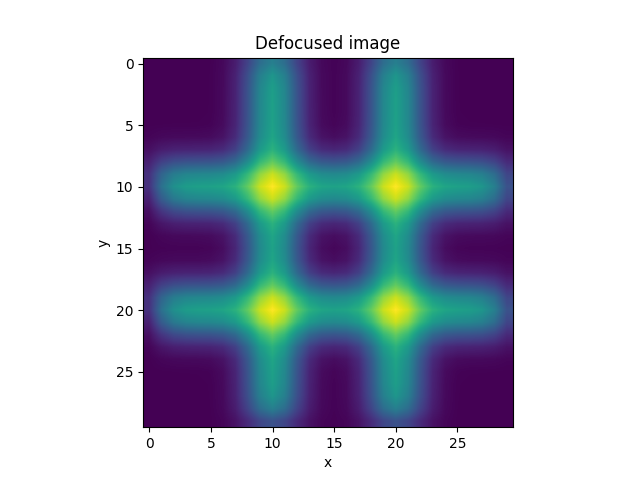
\includegraphics[width=2.2in]{images/defocused.png} &
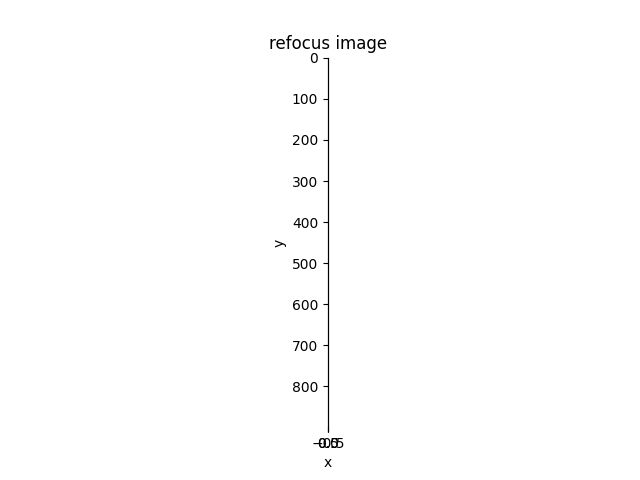
\includegraphics[width=2.2in]{images/refocused.png}
\end{tabular}
\caption{An out-of-focus image (left) and the original image (image) computed from the out-of-focus one, using sparse matrix inversion.}
\end{figure}

When the Hubble telescope was first put into orbit, its mirror was not installed properly and caused the telescope to take pictures out of focus. Until the defect was physically corrected, scientists were able to fix the images using a similar algorithm.

\goodbreak\section{Solvers for nonlinear equations}

\index{non-linear equations}

In this chapter, we are concerned with the problem of solving in $x$ the equation of one variable:

\begin{equation}
f(x) = 0
\end{equation}

\goodbreak\subsection{Fixed-point method}

\index{fixed point method}

It is always possible to reformulate $f(x)=0$ as $g(x)=x$ using, for example, one of the following definitions:
\begin{itemize}
\item $g(x) = f(x)/c+x$ for some constant $c$
\item $g(x) = f(x)/q(x)+x$ for some $q(x)>0$ at the solution of $f(x)=0$
\end{itemize}

We start at $x_0$, an arbitrary point in the domain, and close to the solution we seek. We compute
\begin{eqnarray}
x_1 &=& g(x_0) \\
x_2 &=& g(x_1) \\
x_3 &=& g(x_2) \\
... &=& ...
\end{eqnarray}
We can compute the distance between $x_i$ and $x$ as
\begin{eqnarray}
|x_i - x| &=& |g(x_{i-1})-g(x)| \\
          &=& |g(x)+g"(\xi)(x_{i-1}-x)-g(x)| \\
          &=& |g"(\xi)||x_{i-1}-x|
\end{eqnarray}
where we use {\it de l"Hopital rule} and $\xi$ is a point in between $x$ and $x_{i-1}$.

If the magnitude of the first derivative of $g$, $|g"|$, is less than 1 in a neighborhood of $x$, and if $x_0$ is in such a neighborhood, then

\begin{equation}
|x_i - x| = |g"(\xi)||x_{i-1}-x| < |x_{i-1}-x|
\end{equation}

The $x_i$ series will get closer and closer to the solution $x$.

Here is the process implemented into an algorithm:

%%% META:FILE:nlib/solvers.nim
\begin{lstlisting}[caption={in file: {\ft nlib/solvers.nim}}]
proc solveFixedPoint*(f: proc(x: float): float, x0: float,
                      ap = 1e-6, rp = 1e-4, ns = 100): float =
  let g = proc(x: float): float = f(x) + x
  let Dg = D(g)
  var x = x0
  for k in 0 ..< ns:
    if abs(Dg(x)) >= 1:
      raise newException(ArithmeticDefect, "error D(g)(x)>=1")
    let xOld = x
    x = g(x)
    if k > 2 and norm(xOld - x) < max(ap, norm(x) * rp):
      return x
  raise newException(ArithmeticDefect, "no convergence")
\end{lstlisting}

And here is an example:

\begin{lstlisting}
proc f(x: float): float = (x - 2.0) * (x - 5.0) / 10.0
echo formatFloat(solveFixedPoint(f, 1.0, rp = 0.0), ffDecimal, 4)
# 2.0000
\end{lstlisting}

\goodbreak\subsection{Bisection method}

\index{bisection method}

The goal of the bisection~\cite{bisection} method is to solve $f(x)=0$ when the function is continuous and it is known to change sign in between $x=a$ and $x=b$. The bisection method is the continuous equivalent of the binary search algorithm seen in chapter 3. The algorithm iteratively finds the middle point of the domain $x=(b+a)/2$, evaluates the function there, and decides whether the solution is on the left or the right, thus reducing the size of the domain from $(a, b)$ to $(a, x)$ or $(x, b)$, respectively:

%%% META:FILE:nlib/solvers.nim
\begin{lstlisting}[caption={in file: {\ft nlib/solvers.nim}}]
proc solveBisection*(f: proc(x: float): float, a0, b0: float,
                     ap = 1e-6, rp = 1e-4, ns = 100): float =
  var a = a0
  var b = b0
  var fa = f(a)
  var fb = f(b)
  if fa == 0: return a
  if fb == 0: return b
  if fa * fb > 0:
    raise newException(ArithmeticDefect,
                       "f(a) and f(b) must have opposite sign")
  for k in 0 ..< ns:
    let x = (a + b) / 2.0
    let fx = f(x)
    if fx == 0 or norm(b - a) < max(ap, norm(x) * rp):
      return x
    if fx * fa < 0:
      b = x; fb = fx
    else:
      a = x; fa = fx
  raise newException(ArithmeticDefect, "no convergence")
\end{lstlisting}

Here is how to use it:

\begin{lstlisting}
proc f(x: float): float = (x - 2.0) * (x - 5.0)
echo formatFloat(solveBisection(f, 1.0, 3.0), ffDecimal, 4)
# 2.0000
\end{lstlisting}

\goodbreak\subsection{Newton method}

\index{Newton solver}

The Newton~\cite{newton} algorithm also solves $f(x)=0$. It is faster (on average) than the bisection method because it makes the additional assumption that the function is also differentiable. This algorithm starts from an arbitrary point $x_0$ and approximates the function at that point with its first-order Taylor expansion
\begin{equation}
f(x) \simeq f(x_0) + f'(x_0)(x-x_0)
\end{equation}
and solves it exactly:
\begin{equation}
f(x) = 0 \rightarrow x = x_0 - \frac{f(x_0)}{f'(x_0)}
\end{equation}
thus finding a new and better estimate for the solution. The algorithm iterates the preceding equation, and when it converges, it approximates the exact solution better and better:

%%% META:FILE:nlib/solvers.nim
\begin{lstlisting}[caption={in file: {\ft nlib/solvers.nim}}]
proc solveNewton*(f: proc(x: float): float, x0: float,
                  ap = 1e-6, rp = 1e-4, ns = 20): float =
  var x = x0
  for k in 0 ..< ns:
    let fx = f(x)
    let Dfx = D(f)(x)
    if norm(Dfx) < ap:
      raise newException(ArithmeticDefect, "unstable solution")
    let xOld = x
    x = x - fx / Dfx
    if k > 2 and norm(x - xOld) < max(ap, norm(x) * rp):
      return x
  raise newException(ArithmeticDefect, "no convergence")
\end{lstlisting}

The algorithm is guaranteed to converge if $|f'(x)|>1$ in some neighborhood of the solution and if the starting point is in this neighborhood. It may also converge if this condition is not true. It is likely to fail when $|f'(x)|\simeq 0$ is in the neighborhood of the solution or the starting point because the terms {\ft fx/Dfx} would become very large.

Here is an example:

\begin{lstlisting}
proc f(x: float): float = (x - 2.0) * (x - 5.0)
echo formatFloat(solveNewton(f, 1.0), ffDecimal, 4)
# 2.0000
\end{lstlisting}

\goodbreak\subsection{Secant method}

\index{secant method}

The secant method is very similar to the Newton method, except that $f'(x)$ is replaced by a numerical estimate computed using the current point $x$ and the previous point visited by the algorithm:
\begin{eqnarray}
f'(x_i) &=& \frac{f(x_i)-f(x_{i-1})}{x_i-x_{i-1}} \\
x_{i+i} &=& x_i - \frac{f(x_i)}{f'(x_i)}
\end{eqnarray}
As the algorithm approaches the exact solution, the numerical derivative becomes a better and better approximation for the derivative:

%%% META:FILE:nlib/solvers.nim
\begin{lstlisting}[caption={in file: {\ft nlib/solvers.nim}}]
proc solveSecant*(f: proc(x: float): float, x0: float,
                  ap = 1e-6, rp = 1e-4, ns = 20): float =
  var x = x0
  var fx = f(x)
  var Dfx = D(f)(x)
  for k in 0 ..< ns:
    if norm(Dfx) < ap:
      raise newException(ArithmeticDefect, "unstable solution")
    let xOld = x
    let fxOld = fx
    x = x - fx / Dfx
    if k > 2 and norm(x - xOld) < max(ap, norm(x) * rp):
      return x
    fx = f(x)
    Dfx = (fx - fxOld) / (x - xOld)
  raise newException(ArithmeticDefect, "no convergence")
\end{lstlisting}

Here is an example:

\begin{lstlisting}
proc f(x: float): float = (x - 2.0) * (x - 5.0)
echo formatFloat(solveSecant(f, 1.0), ffDecimal, 4)
# 2.0000
\end{lstlisting}

\goodbreak\section{Optimization in one dimension}

\index{optimization}

While a solver is an algorithm that finds $x$ such that $f(x)=0$, an optimization algorithm is one that finds the maximum or minimum of the function $f(x)$. If the function is differentiable, this is achieved by solving $f'(x)=0$.

For this reason, if the function is differentiable twice, we can simply rename all previous solvers and replace $f(x)$ with $f'(x)$ and $f'(x)$ with $f''(x)$.

\goodbreak\subsection{Bisection method}

\index{bisection method}

%%% META:FILE:nlib/solvers.nim
\begin{lstlisting}[caption={in file: {\ft nlib/solvers.nim}}]
proc optimizeBisection*(f: proc(x: float): float, a, b: float,
                        ap = 1e-6, rp = 1e-4, ns = 100): float =
  solveBisection(D(f), a, b, ap, rp, ns)
\end{lstlisting}

Here is an example:

\begin{lstlisting}
proc f(x: float): float = (x - 2.0) * (x - 5.0)
echo formatFloat(optimizeBisection(f, 2.0, 5.0), ffDecimal, 4)
# 3.5000
\end{lstlisting}

\goodbreak\subsection{Newton method}

\index{Newton optimization}

%%% META:FILE:nlib/solvers.nim
\begin{lstlisting}[caption={in file: {\ft nlib/solvers.nim}}]
proc optimizeNewton*(f: proc(x: float): float, x0: float,
                     ap = 1e-6, rp = 1e-4, ns = 20): float =
  var x = x0
  let f1 = D(f)
  let f2 = DD(f)
  for k in 0 ..< ns:
    let fx = f1(x)
    let Dfx = f2(x)
    if Dfx == 0: return x
    if norm(Dfx) < ap:
      raise newException(ArithmeticDefect, "unstable solution")
    let xOld = x
    x = x - fx / Dfx
    if norm(x - xOld) < max(ap, norm(x) * rp): return x
  raise newException(ArithmeticDefect, "no convergence")
\end{lstlisting}

\begin{lstlisting}
proc f(x: float): float = (x - 2.0) * (x - 5.0)
echo formatFloat(optimizeNewton(f, 3.0), ffDecimal, 3)
# 3.500
\end{lstlisting}

\goodbreak\subsection{Secant method}

\index{secant method}

As in the Newton case, the secant method can also be used to find extrema, by replacing $f$ with $f'$:

%%% META:FILE:nlib/solvers.nim
\begin{lstlisting}[caption={in file: {\ft nlib/solvers.nim}}]
proc optimizeSecant*(f: proc(x: float): float, x0: float,
                     ap = 1e-6, rp = 1e-4, ns = 100): float =
  var x = x0
  let f1 = D(f)
  let f2 = DD(f)
  var fx = f1(x)
  var Dfx = f2(x)
  for k in 0 ..< ns:
    if fx == 0: return x
    if norm(Dfx) < ap:
      raise newException(ArithmeticDefect, "unstable solution")
    let xOld = x
    let fxOld = fx
    x = x - fx / Dfx
    if norm(x - xOld) < max(ap, norm(x) * rp): return x
    fx = f1(x)
    Dfx = (fx - fxOld) / (x - xOld)
  raise newException(ArithmeticDefect, "no convergence")
\end{lstlisting}

\begin{lstlisting}
proc f(x: float): float = (x - 2.0) * (x - 5.0)
echo formatFloat(optimizeSecant(f, 3.0), ffDecimal, 3)
# 3.500
\end{lstlisting}

\goodbreak\subsection{Golden section search}

\index{golden section search}

If the function we want to optimize is continuous but not differentiable, then the previous algorithms do not work. In this case, there is one algorithm that comes to our rescue, the golden section~\cite{golden} search. It is similar to the bisection method, with one caveat; in the bisection method, at each point, we need to know if a function changes sign in between two points, therefore two points are all we need. If instead we are looking for a max or min, we need to know if the function is concave or convex in between those two points. This requires one extra point in between the two. So while the bisection method only needs one point in between $[a, b]$, the golden search needs two points, $x_1$ and $x_2$, in between $[a, b]$, and from them it can determine whether the extreme is in $[a, x_2]$ or in $[x_1, b]$. This is also represented pictorially in fig.~\ref{golden-pic}. The two points are chosen in an optimal way so that at the next iteration, one of the two points can be recycled by leaving the ratio between $x_1-a$ and $b-x_2$ fixed and equal to 1:

%%% META:FILE:nlib/solvers.nim
\begin{lstlisting}[caption={in file: {\ft nlib/solvers.nim}}]
proc optimizeGoldenSearch*(f: proc(x: float): float, a0, b0: float,
                           ap = 1e-6, rp = 1e-4, ns = 100): float =
  var a = a0
  var b = b0
  let tau = (sqrt(5.0) - 1.0) / 2.0
  var x1 = a + (1.0 - tau) * (b - a)
  var x2 = a + tau * (b - a)
  var fa = f(a); var f1 = f(x1); var f2 = f(x2); var fb = f(b)
  for k in 0 ..< ns:
    if f1 > f2:
      a = x1; fa = f1; x1 = x2; f1 = f2
      x2 = a + tau * (b - a); f2 = f(x2)
    else:
      b = x2; fb = f2; x2 = x1; f2 = f1
      x1 = a + (1.0 - tau) * (b - a); f1 = f(x1)
    if k > 2 and norm(b - a) < max(ap, norm(b) * rp): return b
  raise newException(ArithmeticDefect, "no convergence")
\end{lstlisting}

Here is an example:

\begin{lstlisting}
proc f(x: float): float = (x - 2.0) * (x - 5.0)
echo formatFloat(optimizeGoldenSearch(f, 2.0, 5.0), ffDecimal, 3)
# 3.500
\end{lstlisting}

\begin{figure}[ht]
\centering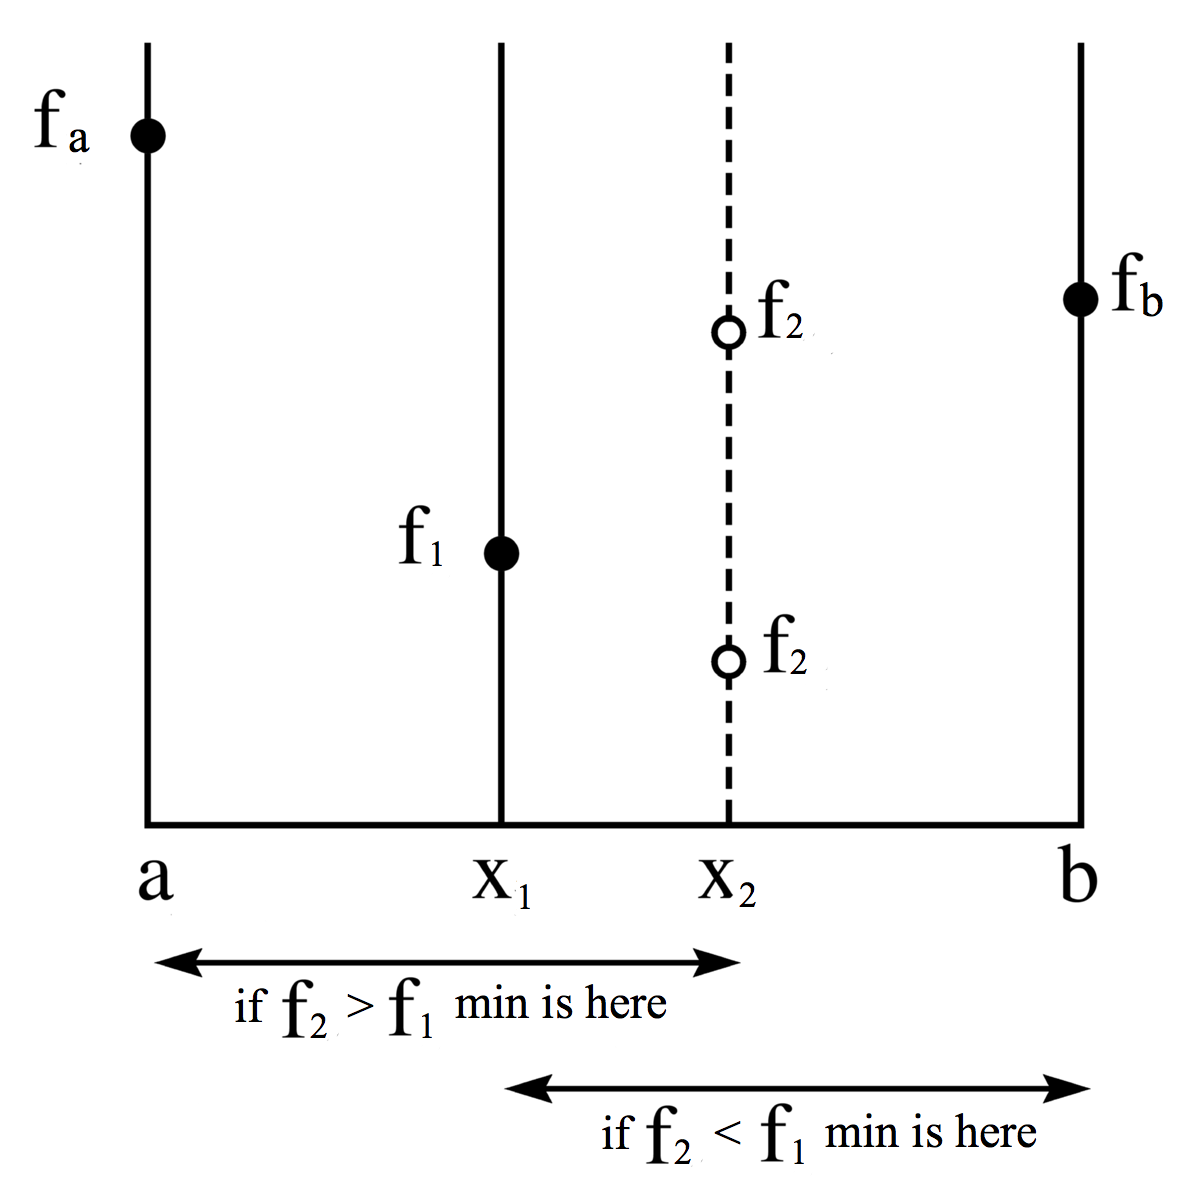
\includegraphics[width=2in]{images/golden.png}
\caption{Pictorial representation of the golden search method. If the function is concave ($f''(x)>0$), then knowledge of the function in 4 points ($a$, $x_1$, $x_2$, $b$) permits us to determine whether a minimum is between $[a, x_2]$ or between $[x_1, b]$.\label{golden-pic}}.
\end{figure}

\goodbreak\section{Functions of many variables}

\index{partial derivative}

To be able to work with functions of many variables, we need to introduce the concept of the partial derivative:

\begin{equation}
\frac{\partial f(\mathbf{x})}{\partial x_i} = \lim_{h \rightarrow 0} \frac{f(\mathbf{x}+\mathbf{h}_i) - f(\mathbf{x}-\mathbf{h}_i)}{2h}
\end{equation}
where $\mathbf{h}_i$ is a vector with components all equal to zero but $h_i = h > 0$.

We can implement it as follows:

%%% META:FILE:nlib/calculus.nim
\begin{lstlisting}[caption={in file: {\ft nlib/calculus.nim}}]
proc partial*(f: proc(x: seq[float]): float, i: int, h = 1e-4):
              proc(x: seq[float]): float =
  result = proc(x: seq[float]): float =
    var x = x
    x[i] += h
    let fPlus = f(x)
    x[i] -= 2.0 * h
    let fMinus = f(x)
    (fPlus - fMinus) / (2.0 * h)

proc partial*(f: proc(x: seq[float]): seq[float], i: int, h = 1e-4):
              proc(x: seq[float]): seq[float] =
  result = proc(x: seq[float]): seq[float] =
    var x = x
    x[i] += h
    let fPlus = f(x)
    x[i] -= 2.0 * h
    let fMinus = f(x)
    result = newSeq[float](fPlus.len)
    for k in 0 ..< fPlus.len:
      result[k] = (fPlus[k] - fMinus[k]) / (2.0 * h)
\end{lstlisting}

Similarly to {\ft D(f)}, we have implemented it in such a way that {\ft partial(f, i)} returns a function that can be evaluated at any point $x$. Also notice that the function $f$ may return a scalar, a matrix, a list, or a tuple. The {\ft if} condition allows the function to deal with the difference between two lists or tuples.

Here is an example:

\begin{lstlisting}
proc f(x: seq[float]): float = 2.0*x[0] + 3.0*x[1] + 5.0*x[1]*x[2]
let df0 = partial(f, 0)
let df1 = partial(f, 1)
let df2 = partial(f, 2)
let x = @[1.0, 1.0, 1.0]
echo (formatFloat(df0(x), ffDecimal, 4),
      formatFloat(df1(x), ffDecimal, 4),
      formatFloat(df2(x), ffDecimal, 4))
# ("2.0000", "8.0000", "5.0000")
\end{lstlisting}

\goodbreak\subsection{Jacobian, gradient, and Hessian}

\index{Jacobian}\index{Gradient}\index{Hessian}

A generic function $f(x_0, x_1, x_2, ...)$ of multiple variables $\mathbf{x}=(x_0, x_1, x_2, ..)$ can be expanded in Taylor series to the second order as

\begin{eqnarray}
f(x_0, x_1, x_2, ...) &=& f(\bar x_0, \bar x_1, \bar x_2, ...) + \\
&& \sum_i \frac{\partial f(\mathbf{\bar x})}{\partial x_i}(x_i-\bar x_i) + \\
&& \sum_{ij} \frac12 \frac{\partial^2 f}{\partial x_i\partial x_j}(\mathbf{\bar x})(x_i-\bar x_i)(x_j-\bar x_j) + ...
\end{eqnarray}

We can rewrite the above expression in terms of the vector $\mathbf{x}$ as follows:

\begin{equation}
f(\mathbf{x}) = f(\mathbf{\bar x}) + \nabla_f(\mathbf{\bar x})(\mathbf{x}-\mathbf{\bar x})
+ \frac12 (\mathbf{x}-\mathbf{\bar x})^t H_f(\mathbf{\bar x})(\mathbf{x}-\mathbf{\bar x}) + ...
\end{equation}

where we introduce the gradient vector

\begin{equation}
\nabla_f(x) \equiv \left(
\begin{tabular}{c}
$\partial f(x)/\partial x_0$ \\
$\partial f(x)/\partial x_1$ \\
$\partial f(x)/\partial x_2$ \\
...
\end{tabular}
\right)
\end{equation}

and the Hessian matrix

\begin{equation}
H_f(x) \equiv \left(
\begin{tabular}{cccc}
$\partial^2 f(x)/\partial x_0\partial x_0$ &
$\partial^2 f(x)/\partial x_0\partial x_1$ &
$\partial^2 f(x)/\partial x_0\partial x_2$ &
... \\
$\partial^2 f(x)/\partial x_1\partial x_0$ &
$\partial^2 f(x)/\partial x_1\partial x_1$ &
$\partial^2 f(x)/\partial x_1\partial x_2$ &
... \\
$\partial^2 f(x)/\partial x_2\partial x_0$ &
$\partial^2 f(x)/\partial x_2\partial x_1$ &
$\partial^2 f(x)/\partial x_2\partial x_2$ &
... \\
... & ... & ... & ...
\end{tabular}
\right)
\end{equation}

Given the definition of partial, we can compute the gradient and the Hessian using the two functions

%%% META:FILE:nlib/calculus.nim
\begin{lstlisting}[caption={in file: {\ft nlib/calculus.nim}}]
proc gradient*(f: proc(x: seq[float]): float,
               x: seq[float], h = 1e-4): Matrix =
  newMatrix(x.len, 1,
    proc(r, c: int): float = partial(f, r, h)(x))

proc hessian*(f: proc(x: seq[float]): float,
              x: seq[float], h = 1e-4): Matrix =
  newMatrix(x.len, x.len,
    proc(r, c: int): float = partial(partial(f, r, h), c, h)(x))
\end{lstlisting}

Here is an example:

\begin{lstlisting}
proc f(x: seq[float]): float = 2.0*x[0] + 3.0*x[1] + 5.0*x[1]*x[2]
echo gradient(f, @[1.0, 1.0, 1.0])
# @[@[1.999999...], @[7.999999...], @[4.999999...]]
echo hessian(f, @[1.0, 1.0, 1.0])
# @[@[0.0, 0.0, 0.0], @[0.0, 0.0, 5.000000...], @[0.0, 5.000000..., 0.0]]
\end{lstlisting}

When dealing with functions returning multiple values like
\begin{equation}
f(\mathbf{x}) = (f_0(\mathbf{x}), f_1(\mathbf{x}), f_2(\mathbf{x}), ...)
\end{equation}

we need to Taylor expand each component:

\begin{equation}
f(\mathbf{x}) =
\left(
\begin{tabular}{c}
$f_0(\mathbf{x})$ \\
$f_1(\mathbf{x})$ \\
$f_2(\mathbf{x})$ \\
...
\end{tabular}
\right) =
\left(
\begin{tabular}{c}
$f_0(\mathbf{\bar x}) + \nabla_{f_0}(\mathbf{x}-\mathbf{\bar x}) + ...$ \\
$f_1(\mathbf{\bar x}) + \nabla_{f_1}(\mathbf{x}-\mathbf{\bar x}) + ...$ \\
$f_2(\mathbf{\bar x}) + \nabla_{f_2}(\mathbf{x}-\mathbf{\bar x}) + ...$ \\
...
\end{tabular}
\right)
\end{equation}

which we can rewrite as

\begin{equation}
f(\mathbf{x}) = f(\mathbf{\bar x}) + J_f(\mathbf{\bar x})(\mathbf{x}-\mathbf{\bar x}) + ... \label{jacobian2}
\end{equation}

where $J_f$ is called Jacobian and is defined as

\begin{equation}
J_f \equiv
\left(
\begin{tabular}{cccc}
$\partial f_0(x)/\partial x_0$ &
$\partial f_0(x)/\partial x_1$ &
$\partial f_0(x)/\partial x_2$ &
... \\
$\partial f_1(x)/\partial x_0$ &
$\partial f_1(x)/\partial x_1$ &
$\partial f_1(x)/\partial x_2$ &
... \\
$\partial f_2(x)/\partial x_0$ &
$\partial f_2(x)/\partial x_1$ &
$\partial f_2(x)/\partial x_2$ &
... \\
... & ... & ... & ...
\end{tabular}
\right)
\end{equation}

which we can implement as follows:

%%% META:FILE:nlib/calculus.nim
\begin{lstlisting}[caption={in file: {\ft nlib/calculus.nim}}]
proc jacobian*(f: proc(x: seq[float]): seq[float],
               x: seq[float], h = 1e-4): Matrix =
  var partials: seq[seq[float]] = @[]
  for c in 0 ..< x.len:
    partials.add partial(f, c, h)(x)
  newMatrix(partials[0].len, x.len,
    proc(r, c: int): float = partials[c][r])
\end{lstlisting}

Here is an example:

\begin{lstlisting}
proc f(x: seq[float]): seq[float] =
  @[2.0*x[0] + 3.0*x[1] + 5.0*x[1]*x[2], 2.0*x[0]]
echo jacobian(f, @[1.0, 1.0, 1.0])
# @[@[1.9999999..., 7.999999..., 4.9999999...], @[1.9999999..., 0.0, 0.0]]
\end{lstlisting}

\goodbreak\subsection{Newton method (solver)}

\index{Newton solver!multidimensional}

We can now solve eq.~\ref{jacobian2} iteratively as we did for the one-dimensional Newton solver with only one change---the first derivative of $f$ is replaced by the Jacobian:

%%% META:FILE:nlib/solvers.nim
\begin{lstlisting}[caption={in file: {\ft nlib/solvers.nim}}]
proc solveNewtonMulti*(f: proc(x: seq[float]): seq[float],
                       x0: seq[float],
                       ap = 1e-6, rp = 1e-4, ns = 20): seq[float] =
  ## Multidimensional Newton solver. Finds `x` such that `f(x) == 0`.
  var x = newMatrix(x0)
  for k in 0 ..< ns:
    let fx = newMatrix(f(x.flatten()))
    let J = jacobian(f, x.flatten())
    if norm(J) < ap:
      raise newException(ArithmeticDefect, "unstable solution")
    let xOld = x
    x = x - (1.0 / J) * fx
    if k > 2 and norm(x - xOld) < max(ap, norm(x) * rp):
      return x.flatten()
  raise newException(ArithmeticDefect, "no convergence")
\end{lstlisting}

Here is an example:

\begin{lstlisting}
proc f(x: seq[float]): seq[float] =
  @[x[0] + x[1], x[0] + x[1] ^ 2 - 2.0]
echo solveNewtonMulti(f, @[0.0, 0.0])
# @[1.0..., -1.0...]
\end{lstlisting}

\goodbreak\subsection{Newton method (optimize)}

\index{Newton optimizer!multi-dimensional}

As for the one-dimensional case, we can approximate $f(\mathbf{x})$ with its Taylor expansion at the first order, 
\begin{equation}
f(\mathbf{x}) = f(\mathbf{\bar x}) + \nabla_f(\mathbf{\bar x})(\mathbf{x}-\mathbf{\bar x}) +
\frac12 (\mathbf{x}-\mathbf{\bar x})^t H_f(\mathbf{\bar x})(\mathbf{x}-\mathbf{\bar x})
\end{equation}
set its derivative to zero, and solve it, thus obtaining
\begin{equation}
\mathbf{x} = \mathbf{\bar x} - H^{-1}_f \nabla_f
\end{equation}
which constitutes the core of the multidimensional Newton optimizer:

%%% META:FILE:nlib/solvers.nim
\begin{lstlisting}[caption={in file: {\ft nlib/solvers.nim}}]
proc optimizeNewtonMulti*(f: proc(x: seq[float]): float,
                          x0: seq[float],
                          ap = 1e-6, rp = 1e-4, ns = 20): seq[float] =
  ## Multidimensional Newton optimizer. Finds extremum of `f`.
  var x = newMatrix(x0)
  for k in 0 ..< ns:
    let grad = gradient(f, x.flatten())
    let H = hessian(f, x.flatten())
    if norm(H) < ap:
      raise newException(ArithmeticDefect, "unstable solution")
    let xOld = x
    x = x - (1.0 / H) * grad
    if k > 2 and norm(x - xOld) < max(ap, norm(x) * rp):
      return x.flatten()
  raise newException(ArithmeticDefect, "no convergence")
\end{lstlisting}

\begin{lstlisting}
proc f(x: seq[float]): float = (x[0] - 2.0) ^ 2 + (x[1] - 3.0) ^ 2
echo optimizeNewtonMulti(f, @[0.0, 0.0])
# @[2.0, 3.0]
\end{lstlisting}

\goodbreak\subsection{Improved Newton method (optimize)}

We can further improve the Newton multidimensional optimizer by using the following technique. At each step, if the next guess does not reduce the value of $f$, we revert to the previous point, and we perform a one-dimensional Newton optimization along the direction of the gradient. This method greatly increases the stability of the multidimensional Newton optimizer:

%%% META:FILE:nlib/solvers.nim
\begin{lstlisting}[caption={in file: {\ft nlib/solvers.nim}}]
proc optimizeNewtonMultiImproved*(
    f: proc(x: seq[float]): float, x0: seq[float],
    ap = 1e-6, rp = 1e-4, ns = 20, hStart = 10.0): seq[float] =
  ## Newton optimizer with line-search fallback to steepest descent.
  var x = newMatrix(x0)
  var fx = f(x.flatten())
  var h = hStart
  for k in 0 ..< ns:
    let grad = gradient(f, x.flatten())
    let H = hessian(f, x.flatten())
    if norm(H) < ap:
      raise newException(ArithmeticDefect, "unstable solution")
    var fxOld = fx
    var xOld = x
    x = x - (1.0 / H) * grad
    fx = f(x.flatten())
    while fx > fxOld:
      fx = fxOld; x = xOld
      let normGrad = norm(grad)
      xOld = x
      x = x - grad * (h / normGrad)
      fxOld = fx
      fx = f(x.flatten())
      h = h / 2.0
    h = norm(x - xOld) * 2.0
    if k > 2 and h / 2.0 < max(ap, norm(x) * rp):
      return x.flatten()
  raise newException(ArithmeticDefect, "no convergence")
\end{lstlisting}

\goodbreak\section{Nonlinear fitting}

Finally, we have all the ingredients to implement a very generic fitting function that will work linear and nonlinear least squares.

Here we consider a generic experiment or simulated experiment that generates points of the form $(x_i, y_i \pm \delta y_i)$. Our goal is to minimize the $\chi^2$ defined as
\begin{equation}
\chi^2(\mathbf{a}, \mathbf{b}) = \sum _i \left|
\frac{y_i - f(x_i, \mathbf{a}, \mathbf{b})}{\delta y_i}
\right|^2
\end{equation}
where the function $f$ is known but depends on unknown parameters $\mathbf{a}=(a_0, a_1, ...)$ and $\mathbf{b}=(b_0, b_1, ...)$. In terms of these parameters, the function $f$ can be written as follows:
\begin{equation}
f(x, \mathbf{a}, \mathbf{b}) = \sum_j a_j f_j(x, \mathbf{b})
\end{equation}
Here is an example:
\begin{equation}
f(x, \mathbf{a}, \mathbf{b}) = a_0 e^{-b_0 x} + a_1 e^{-b_1 x} + a_2 e^{-b_2 x} + ...
\end{equation}
The goal of our algorithm is to efficiently determine the parameters $\mathbf{a}$ and $\mathbf{b}$ that minimize the $\chi^2$.

We proceed by defining the following two quantities:

\begin{equation}
\mathbf{z} = \left(
\begin{tabular}{c}
$y_0$ / $\delta y_0$ \\
$y_1$ / $\delta y_1$ \\
$y_2$ / $\delta y_2$ \\
...
\end{tabular}
\right)
\end{equation}

and

\begin{equation}
A(\mathbf{b}) = \left(
\begin{tabular}{cccc}
$f_0(x_0, \mathbf{b})/\delta y_0$ &
$f_1(x_0, \mathbf{b})/\delta y_0$ &
$f_2(x_0, \mathbf{b})/\delta y_0$ & ... \\
$f_0(x_1, \mathbf{b})/\delta y_1$ &
$f_1(x_1, \mathbf{b})/\delta y_1$ &
$f_2(x_1, \mathbf{b})/\delta y_1$ & ... \\
$f_0(x_2, \mathbf{b})/\delta y_2$ &
$f_1(x_2, \mathbf{b})/\delta y_2$ &
$f_2(x_2, \mathbf{b})/\delta y_2$ & ... \\
... & ... & ... & ...
\end{tabular}
\right)
\end{equation}

In terms of $A$ and $z$, the $\chi^2$ can be rewritten as

\begin{equation}
\chi^2(\mathbf{a}, \mathbf{b}) = \left| A(\mathbf{b}) \mathbf{a} - \mathbf{z} \right|^2
\end{equation}

We can minimize this function in $a$ using the linear least squares algorithm, exactly:

\begin{equation}
\mathbf{a}(\mathbf{b}) = (A(\mathbf{b}) A(\mathbf{b})^t)^{-1}(A(\mathbf{b})^t z)
\end{equation}

We define a function that returns the minimum $\chi^2$ for a fixed input $\mathbf{b}$:

\begin{equation}
g(\mathbf{b}) =
\min_{\mathbf{a}}
\chi^2(\mathbf{a}, \mathbf{b}) =
\chi^2(\mathbf{a}(\mathbf{b}), \mathbf{b}) = \left|
A(\mathbf{b})\mathbf{a}(\mathbf{b}) - \mathbf{z}
\right|^2
\end{equation}

Therefore we have reduced the original problem to a simple problem by reducing the number of unknown parameters from $N_a+N_b$ to $N_b$.

The following code takes as input the {\ft data} as a list of $(x_i, y_i, \delta y_i)$, a list of functions (or a single function), and a guess for the $\mathbf{b}$ values. If the {\ft fs} argument is not a list but a single function, then there is no $\mathbf{a}$ to compute, and the function proceeds by minimizing the $\chi^2$ using the improved Newton optimizer (the one-dimensional or the improved multidimensional one, as appropriate). If the argument $\mathbf{b}$ is missing, then the fitting parameters are all linear, and the algorithm reverts to regular linear least squares. Otherwise, run the more complex algorithm described earlier:

%%% META:FILE:nlib/fitting.nim
\begin{lstlisting}[caption={in file: {\ft nlib/fitting.nim}}]
type
  NonlinearFit* = proc(b: seq[float], x: float): float

proc fit*(data: seq[(float, float, float)],
          fs: seq[NonlinearFit],
          b0: seq[float],
          ap = 1e-6, rp = 1e-4, ns = 200,
          constraint: proc(b: seq[float]): float = nil
          ): (seq[float], float) =
  ## Generic linear/nonlinear chi^2 fit. Returns (parameters, chi2).
  let na = fs.len
  proc core(b: seq[float]): (seq[float], float) =
    let A = newMatrix(data.len, na,
      proc(r, c: int): float = fs[c](b, data[r][0]) / data[r][2])
    let z = newMatrix(data.len, 1,
      proc(r, c: int): float = data[r][1] / data[r][2])
    let a = (1.0 / (A.T * A)) * (A.T * z)
    let chi2Val = norm(A * a - z) ^ 2
    (a.flatten(), chi2Val)
  proc g(b: seq[float]): float =
    let (_, chi2v) = core(b)
    var s = chi2v
    if constraint != nil: s += constraint(b)
    s
  let b = optimizeNewtonMultiImproved(g, b0, ap, rp, ns)
  let (a, chi2v) = core(b)
  (a & b, chi2v)
\end{lstlisting}

Here is an example:

\begin{lstlisting}
var data: seq[(float, float, float)] = @[]
for i in 1 ..< 10:
  let fi = float(i)
  data.add (fi, fi + 2.0 * fi^2 + 300.0 / (fi + 10.0), 2.0)
let fs: seq[NonlinearFit] = @[
  proc(b: seq[float], x: float): float = x,
  proc(b: seq[float], x: float): float = x * x,
  proc(b: seq[float], x: float): float = 1.0 / (x + b[0]),
]
let (ab, chi2) = fit(data, fs, @[5.0])
echo ab, " ", chi2
# @[0.999..., 2.000..., 300.000..., 10.000...] ...
\end{lstlisting}

\index{a priori}\index{Bayesian statistics}

In the preceding implementation, we added a somewhat mysterious argument {\ft constraint}. This is a function of $\mathbf{b}$, and its output gets added to the value of $\chi^2$, which we are minimizing. By choosing the appropriate function, we can set constraints about the expected values $b$. These constraints represent a priori knowledge about the parameters, that is, knowledge that does not come from the data being fitted.

For example, if we know that $b_i$ must be close to some $\bar b_i$ with some uncertainty $\delta b_i$, then we can use
\begin{lstlisting}
proc constraint(b, barB, deltaB: seq[float]): float =
  for i in 0 ..< b.len:
    result += ((b[i] - barB[i]) / deltaB[i]) ^ 2
\end{lstlisting}

and pass the preceding function as a constraint.
From a practical effect, this stabilizes our fit. From a theoretical point of view, the $\bar b_i$ are the {\it priors} of Bayesian statistics.

\goodbreak\section{Integration}

\index{integration!numerical}\index{integration!trapezoid}

Consider the integral of $f(x)$ for $x$ in domain $[a, b]$, which we normally represent as

\begin{equation}
I = \int_a^b f(x)dx
\end{equation}
 and which measures the area under the curve $y=f(x)$ delimited on the left by $x=a$ and on the right by $x=b$.

\begin{figure}[ht]
\centering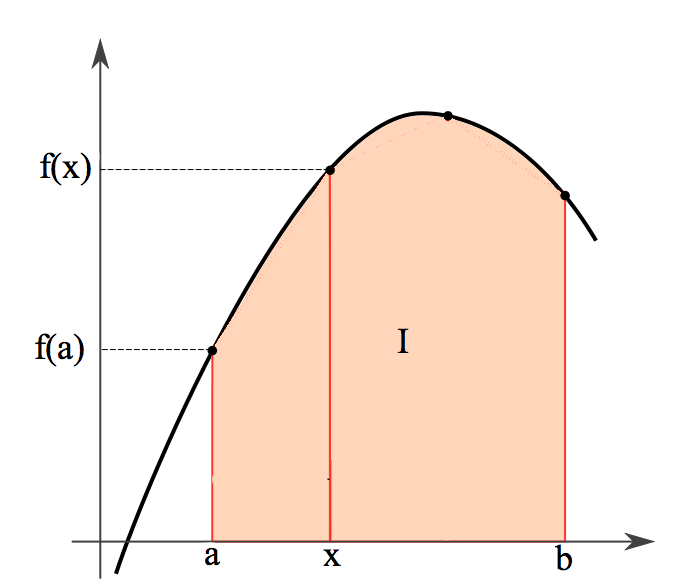
\includegraphics[width=2in]{images/integral1.png}
\caption{Visual representation of the concept of an integral as the area under a curve.}
\end{figure}

As we did in the previous subsection, we can approximate the possible values taken by $x$ as discrete values $x\equiv h i$, where $h=(b-a)/n$. At those values, the function $f$ evaluates to $f_i \equiv f(h i)$. Thus the integral can be approximated as a sum of trapezoids:

\begin{equation}
  I_n \simeq \sum_{i=0}^{i<n} \frac{h}{2}(f_i+f_{i+1})
\end{equation}

\begin{figure}[ht]
\centering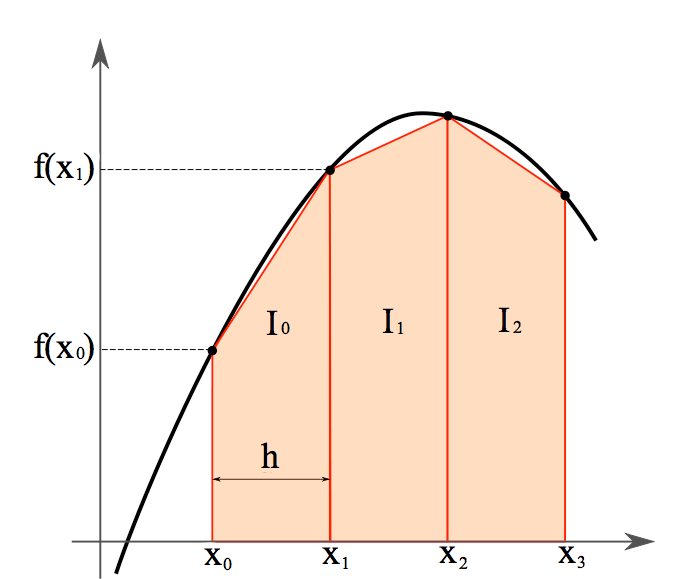
\includegraphics[width=2in]{images/integral2.png}
\caption{Visual representation of the trapezoid method for numerical integration.}
\end{figure}

If a function is discontinuous only in a finite number of points in the domain $[a, b]$, then the following limit exists:

\begin{equation}
\lim_{n\rightarrow\infty} I_n \rightarrow I
\end{equation}

We can implement the naive integration as a function of $N$ as follows:

%%% META:FILE:nlib/integration.nim
\begin{lstlisting}[caption={in file: {\ft nlib/integration.nim}}]
proc integrateNaive*(f: proc(x: float): float,
                     a, b: float, n = 20): float =
  ## Trapezoidal-rule integration of `f` over `[a, b]` with `n` slices.
  let h = (b - a) / float(n)
  result = h / 2.0 * (f(a) + f(b))
  for i in 1 ..< n:
    result += h * f(a + h * float(i))
\end{lstlisting}

And here we implement the limit by doubling the number of points until convergence is achieved:

%%% META:FILE:nlib/integration.nim
\begin{lstlisting}[caption={in file: {\ft nlib/integration.nim}}]
proc integrate*(f: proc(x: float): float, a, b: float,
                ap = 1e-4, rp = 1e-4, ns = 20): float =
  ## Iteratively-refined trapezoidal integration.
  var I = integrateNaive(f, a, b, 1)
  for k in 1 ..< ns:
    let IOld = I
    I = integrateNaive(f, a, b, 2 ^ k)
    if k > 2 and norm(I - IOld) < max(ap, norm(I) * rp):
      return I
  raise newException(ArithmeticDefect, "no convergence")
\end{lstlisting}

We can test the convergence as follows:

\begin{lstlisting}
echo integrateNaive(sin, 0.0, 3.0, n = 2)   # 1.6020...
echo integrateNaive(sin, 0.0, 3.0, n = 4)   # 1.8958...
echo integrateNaive(sin, 0.0, 3.0, n = 8)   # 1.9666...
echo integrate(sin, 0.0, 3.0)               # 1.9899...
echo 1.0 - cos(3.0)                         # 1.9899...
\end{lstlisting}

\goodbreak\subsection{Quadrature}

\index{integration!quadrature}

In the previous integration, we divided the domain $[a, b]$ into subdomains, and we computed the area under the curve $f$ in each subdomain by approximating it with a trapezoid; for example, we approximated the function in between $x_i$ and $x_{i+1}$ with a straight line. We can do better by approximating the function with a polynomial of arbitrary degree $n$ and then compute the area in the subdomain by explicitly integrating the polynomial.

This is the basic idea of quadrature. For a subdomain delimited by $(0, 1)$, we can impose
\begin{eqnarray}
\int_0^1 1\textrm{d}x &= h &= \sum_i c_i (i/n)^0 \\
\int_0^1 x\textrm{d}x &= h^2/2 &= \sum_i c_i (i/n)^1 \\
... & ... & ... \\
\int_0^1 x^{n-1}\textrm{d}x &= h^n/n &= \sum_i c_i (i/n)^2
\end{eqnarray}
where $c_i$ are coefficients to be determined:

\index{class!QuadratureIntegrator}

%%% META:FILE:nlib/integration.nim
\begin{lstlisting}[caption={in file: {\ft nlib/integration.nim}}]
type
  QuadratureIntegrator* = ref object
    w*: Matrix

proc newQuadratureIntegrator*(order = 4): QuadratureIntegrator =
  let h = 1.0 / float(order - 1)
  let A = newMatrix(order, order,
    proc(r, c: int): float = (float(c) * h) ^ r)
  let s = newMatrix(order, 1,
    proc(r, c: int): float = 1.0 / float(r + 1))
  result = QuadratureIntegrator(w: (1.0 / A) * s)

proc integrate*(q: QuadratureIntegrator,
                f: proc(x: float): float, a, b: float): float =
  let order = q.w.nrows
  let h = (b - a) / float(order - 1)
  for i in 0 ..< order:
    result += q.w[i, 0] * f(a + float(i) * h)
  result *= (b - a)

proc integrateQuadratureNaive*(f: proc(x: float): float,
                               a, b: float, n = 20, order = 4): float =
  let h = (b - a) / float(n)
  let q = newQuadratureIntegrator(order = order)
  for i in 0 ..< n:
    result += q.integrate(f, a + float(i) * h,
                            a + float(i) * h + h)
\end{lstlisting}

Here is an example of usage:

\begin{lstlisting}
echo integrateQuadratureNaive(sin, 0.0, 3.0, n = 2, order = 2) # 1.602...
echo integrateQuadratureNaive(sin, 0.0, 3.0, n = 2, order = 3) # 1.993...
echo integrateQuadratureNaive(sin, 0.0, 3.0, n = 2, order = 4) # 1.991...
\end{lstlisting}

\newpage
\section{Fourier transforms}

A function with a domain over a finite interval $[a, b]$ can be approximated with a vector. For example, consider a function $f(x)$ with domain $[0, T]$. We can sample the function at points $x_k = a+(b-a)k/N$ and represent the discretized function with a vector
\begin{equation}
\mathbf{u}_f \equiv \{cf(x_0), cf(x_1), cf(x_2), ... cf(x_N)\}
\end{equation}
where $c$ is an arbitrary constant that we choose to be $c=\sqrt{(b-a)/N}$. This choice simplifies our later algebra.
Summarizing, we define
\begin{equation}
u_{fk} \equiv \sqrt{\frac{b-a}{N}}f(x_k)
\end{equation}

Given any two functions, we can define their scalar product as the limit of $N\rightarrow\infty$ of the scalar product between their corresponding vectors:

\begin{equation}
f \cdot g \equiv \lim_{N\rightarrow\infty} \mathbf{u}_f \cdot \mathbf{u}_g =
\lim_{N\rightarrow\infty} \frac{b-a}{N} \sum_k f(x_k) g(x_k)
\end{equation}

Using the definition of integral, it can be proven that, in the limit $N\rightarrow\infty$, this is equivalent to

\begin{equation}
f \cdot g = \int_a^b f(x) g(x) dx
\end{equation}

This is because we have chosen $c$ such that $c^2$ is the width of a rectangle in the Riemann integration.

From now on, we will omit the $f$ subscript in $\mathbf{u}$ and simply use different letters for vectors representing different sampled functions ($\mathbf{u}$, $\mathbf{v}$, $\mathbf{b}$, etc.).

Because we are interested in numerical algorithms, we will keep $N$ finite and work with the sum instead of the integral.

Given a fixed $N$, we can always find $N$ vectors $\mathbf{b}_0, \mathbf{b}_1...\mathbf{b}_{N_1}$ that are linearly independent, normalized, and orthogonal, that is, 

\begin{equation}
\mathbf{b}_i \cdot \mathbf{b}_j = \sum_k b_{ik} b_{ik} = \delta_{ij}
\end{equation}

Here $b_{jk}$ is the $k$ component of vector $\mathbf{b}_j$ and $\delta_{ij}$ is the Kroneker delta defined as 0 when $i\neq j$ and 1 when $i == j$.

Any set of vectors $\{\mathbf{b}_j\}$ meeting the preceding condition is called an orthonormal basis. Any other vector $\mathbf{u}$ can be represented by its projections over the basis vectors:

\begin{equation}
  u_i = \sum_i v_j b_{ji}
\end{equation}

where $v_j$ is the projection of $u$ along $\mathbf{b}_j$, which can be computed as
\begin{equation}
  v_j = \sum_i u_i b_{ji}
\end{equation}

In fact, by direct substitution, we obtain

\begin{eqnarray}
  v_j &=& \sum_k u_k b_{jk} \\
      &=& \sum_k (\sum_i v_i b_{ik}) b_{jk} \\
      &=& \sum_i v_i (\sum_k b_{ik} b_{jk}) \\
      &=& \sum_i v_i \delta_{ij} \\
      &=& v_j
\end{eqnarray}

In other words, once we have a basis of vectors, the vector $\mathbf{u}$ can be represented in terms of the vector $\mathbf{v}$ of $v_j$ coefficients and, conversely, $\mathbf{v}$ can be computed from $\mathbf{u}$; $\mathbf{u}$ and $\mathbf{v}$ contain the same information.

The transformation from $\mathbf{u}$ to $\mathbf{v}$, and vice versa, is a linear transformation. We call $T^+$ the transformation from $\mathbf{u}$ to $\mathbf{v}$  and $T^-$ its inverse:

\begin{equation}
\mathbf{v} = T^+(\mathbf{u}) \qquad
\mathbf{u} = T^-(\mathbf{v})
\end{equation}

From the definition, and without attempting any optimization, we can implement these operators as follows:

\begin{lstlisting}
proc transform(u: seq[float], b: seq[seq[float]]): seq[float] =
  for bi in b:
    var s = 0.0
    for k in 0 ..< u.len: s += u[k] * bi[k]
    result.add s

proc antitransform(v: seq[float], b: seq[seq[float]]): seq[float] =
  result = newSeq[float](v.len)
  for k in 0 ..< v.len:
    var s = 0.0
    for i, bi in b: s += v[i] * bi[k]
    result[k] = s
\end{lstlisting}

Here is an example of usage:

\begin{lstlisting}
proc makeBasis(N: int): seq[seq[float]] =
  for j in 0 ..< N:
    var row = newSeq[float](N)
    row[j] = 1.0
    result.add row
let b = makeBasis(4)
echo b
# @[@[1.0, 0.0, 0.0, 0.0], @[0.0, 1.0, 0.0, 0.0], ...]
let u = @[1.0, 2.0, 3.0, 4.0]
let v = transform(u, b)
echo antitransform(v, b)
# @[1.0, 2.0, 3.0, 4.0]
\end{lstlisting}

Of course, this example is trivial because of the choice of basis which makes $v$ the same as $u$. Yet our argument works for any basis $\mathbf{b}_i$. In particular, we can make the following choice:


\begin{equation}
b_{ji} = \frac{1}{\sqrt{2\pi}} e^{2\pi I ij/N}
\end{equation}

where $I$ is the imaginary unit. With this choice, the $T^+$ and $T^-$ functions become

\begin{eqnarray}
v_j &\stackunder{FT^+}{=}& N^{-\frac12} \sum_i u_i e^{2\pi I ij/N} \\
\label{fourierd1}
u_i &\stackunder{FT^-}{=}& N^{-\frac12} \sum_j v_j e^{-2\pi I ij/N}
\label{fourierd2}
\end{eqnarray}

and they take the names of Fourier transform and anti-transform~\cite{fourier}, respectively;
we can implement them as follows:

\begin{lstlisting}
import std/complex

proc fourier(u: seq[Complex64], sign = 1): seq[Complex64] =
  let N = u.len
  let coeff = 1.0 / sqrt(float(N))
  let omega = complex(0.0, 2.0 * PI * float(sign) / float(N))
  result = newSeq[Complex64](N)
  for j in 0 ..< N:
    var s = complex(0.0, 0.0)
    for i in 0 ..< N:
      s = s + complex(coeff, 0.0) * u[i] *
              exp(omega * complex(float(i * j), 0.0))
    result[j] = s

proc antiFourier(v: seq[Complex64]): seq[Complex64] = fourier(v, sign = -1)
\end{lstlisting}

Here {\ft complex(0.0, 1.0)} represents the imaginary unit $I$ in Nim's {\ft std/complex} module, and {\ft exp} on a {\ft Complex64} is the complex exponential.

Notice how the transformation works even when $\mathbf{u}$ is a vector of complex numbers.

Something special happens when $u$ is real:
\begin{eqnarray}
Re(v_j) &=& +Re(v_{N-j-1}) \\
Im(v_j) &=& -Im(v_{N-j-1})
\end{eqnarray}

We can speed up the code even more using recursion and by observing that if $N$ is a power of $2$, then

\begin{eqnarray}
v_j &=& N^{-\frac12} \sum_i u_{2i} e^{2\pi I (2i)j/N} + \\
             &&  N^{-\frac12} \sum_i u_{2i+1} e^{2\pi I (2i+1)j/N} \\
             &=& 2^{-\frac12} ( v_j^{even} + e^{2\pi j/N} v_j^{even} )
\end{eqnarray}

where $v_j^{even}$ is the Fourier transform of the even terms and $v_j^{odd}$ is the Fourier transform of the odd terms.

The preceding recursive expression can be implemented using dynamic programming, thus obtaining


\begin{lstlisting}
import std/complex

proc fastFourier(u: seq[Complex64], sign = 1): seq[Complex64] =
  let N = u.len
  let sqrtN = sqrt(float(N))
  result = newSeq[Complex64](N)
  for i in 0 ..< N:
    result[i] = u[i] / complex(sqrtN, 0.0)
  var k = N div 2
  while k > 0:
    let omega = exp(complex(0.0, 2.0 * PI * float(sign * k) / float(N)))
    for i in 0 ..< N:
      let j = i xor k
      if i < k:
        let ik = i div k
        let jk = j div k
        let vi = result[i]
        let vj = result[j]
        result[i] = vi + pow(omega, complex(float(ik), 0.0)) * vj
        result[j] = vi + pow(omega, complex(float(jk), 0.0)) * vj
    k = k div 2

proc fastAntiFourier(v: seq[Complex64]): seq[Complex64] =
  fastFourier(v, sign = -1)
\end{lstlisting}

This implementation of the Fourier transform is equivalent to the previous one in the sense that it produces the same result (up to numerical issues), but it is faster as it runs in $\Theta(N \log_2 N)$ versus $\Theta(N^2)$ of the naive implementation. Here \verb!i ^ j!
is a binary operator, specifically a XOR. For each binary digit of $i$, it returns a flipped bit if the corresponding bit in $j$ is 1. For example:

\begin{lstlisting}
i  : 10010010101110
j  : 00010001000010
i^j: 10000011001110
\end{lstlisting}

\section{Differential equations}

In this section, we deal specifically with differential equations of the following form:

\begin{equation}
a_0 f(x) + a_1 f'(x) + a_2 f''(x) + ... = g(x) \label{diffeq}
\end{equation}

where $f(x)$ is an unknown function to be determined; $f'$, $f''$, and so on, are its derivatives; $a_i$ are known input coefficients; and $g(x)$ is a known input function:

\begin{equation}
f''(x) - 4 f'(x) + f(x) = sin(x)
\end{equation}

In this case, $a_2(x) = 1$, $a_1(x) = -4$, $a_0(x) = 1$, and $g(x) = \sin(x)$.

This can be solved using Fourier transforms by observing that if the Fourier transform of $f(x)$ is $\tilde f(y)$, then the Fourier transform of $f'(x)$ is $iy\tilde f(y)$.

Hence, if we Fourier transform both the left and right side of

\begin{equation}
\sum _k a_k f^{(k)}(x) = g(x)
\end{equation}

we obtain

\begin{equation}
(\sum _k a_k (i y)^k) \tilde f(y) = \tilde g(y)
\end{equation}

therefore $f(x)$ is the anti-Fourier transform of

\begin{equation}
\tilde f(y) = \frac{\tilde g(y)}{(\sum _k a_k (i y)^k)}
\end{equation}

In one equation, the solution of eq.~\ref{diffeq} is

\begin{equation}
f(x) = T^-(T^+(g)/(\sum _k a_k (iy)^k))
\end{equation}

This is fine and useful when the Fourier transformations are easy to compute.

A more practical numerical solution is the following. We define

\begin{equation}
y_i(x) \equiv f^{(i)}(x)
\end{equation}

and we rewrite the differential equation as

\begin{eqnarray}
y"_0 &=& y_1 \\
y"_1 &=& y_2 \\
y"_2 &=& y_3 \\
... && ... \\
y"_{N-1} &=& y_N = (g(x)-\sum_{k<N} a_k y_k(x))/a_N(x)
\end{eqnarray}

or equivalently

\begin{equation}
\mathbf{y}" = F(\mathbf{y})
\end{equation}

where

\begin{equation}
F(\mathbf{y}) = \mathbf{y}+\left(\begin{tabular}{c}
$y_1$ \\
$y_2$ \\
$y_3$ \\
... \\
$(g(x)-\sum_{k<N} a_k(x)y_k(x))/a_N(x)$
\end{tabular}\right)
\end{equation}

\index{Euler method}
The naive solution is due to Euler:

\begin{equation}
\mathbf{y}(x+h) = \mathbf{y}(x) + hF(\mathbf{y}, x)\label{euler}
\end{equation}

The solution is found by iterating the latest equation. Here $h$ is an arbitrary discretization step. Euler"s method works even if the $a_k$ coefficients depend on $x$.

\index{Runge--Kutta method}
 Although the Euler integrator works in theory, its systematic error adds up and does not disappear in the limit $h\rightarrow 0$. More accurate integrators are the Runge--Kutta and the Adams--Bashforth. In the fourth-order Runge--Kutta, the {\it classical Runge--Kutta method}, we also solve the differential equation by iteration, except that eq.~\ref{euler} is replaced with

\begin{equation}
\mathbf{y}(x+h) = \mathbf{y}(x) + h/6 (\mathbf{k}_1+2\mathbf{k}_2+2\mathbf{k}_3+\mathbf{k}_4)\label{rungekatta}
\end{equation}
where
\begin{eqnarray}
\mathbf{k}_1 &=& F(\mathbf{y}, x) \\
\mathbf{k}_2 &=& F(\mathbf{y}+h k_1/2, x+h/2) \\
\mathbf{k}_3 &=& F(\mathbf{y}+h k_2/2, x+h/2) \\
\mathbf{k}_4 &=& F(\mathbf{y}+h k_3, x+h)
\end{eqnarray}

\chapter{Probability and Statistics}

\goodbreak\section{Probability}

\index{probability}\index{statistics}

Probability derives from the Latin {\it probare} (to prove or to test). The word
probably means roughly ``likely to occur'' in the case of possible future
occurrences or ``likely to be true'' in the case of inferences from
evidence. See also probability theory.

What mathematicians call probability is the mathematical theory we use to
describe and quantify uncertainty. In a larger context, the word {\it probability}
is used with other concerns in mind. Uncertainty can be due to our
ignorance, deliberate mixing or shuffling, or due to the essential
randomness of Nature. In any case, we measure the uncertainty of events on a
scale from zero (impossible events) to one (certain events or no
uncertainty).

There are three standard ways to define probability:

\begin{itemize}
\item  (frequentist) Given an experiment and a set of possible outcomes $S$, 
the probability of an event $A\subset S$ is computed by repeating the
experiment $N$ times, counting how many times the event $A$ is realized, $N_A
$, then taking the limit
\begin{equation}
\textrm{Prob}(A)\equiv \lim_{N\rightarrow \infty }\frac{N_A}N
\end{equation}
This definition actually requires that one performs an experiment, 
if not an infinite, then a number of times.

\item  (a priori) Given an experiment and a set of possible outcomes $S$
with cardinality $c(S)$, the probability of an event $A\subset S$ is defined
as
\begin{equation}
\textrm{Prob}(A)\equiv \frac{c(A)}{c(S)}
\end{equation}
This definition is ambiguous because it assumes that each ``atomic'' event $%
x\in S$ has the same a priori probability and therefore the definition
itself is circular. Nevertheless we use this definition in many practical
circumstances. What is the probability that when rolling a dice we will get an even
number? The space of possible outcomes is $S=\{1, 2, 3, 4, 5, 6\}$ and $A=\{2, 4, 6\}
$ therefore $\textrm{Prob}(A)=c(A)/c(S)=3/6=1/2$. This analysis works for an ideal die
and ignores the fact that a real dice may be biased. The former definition
takes into account this possibility, whereas the latter does not.

\item  (axiomatic definition) Given an experiment and a set of possible
outcomes $S$, the probability of an event $A\subset S$ is a number $\textrm{Prob}(A)\in
[0, 1]$ that satisfies the following conditions: $\textrm{Prob}(S)=1$; $\textrm{Prob}(A_1\cup
A_2)=\textrm{Prob}(A_1)+\textrm{Prob}(A_2)$ if $A_1\cap A_2=0$.
\end{itemize}

In some sense, probability theory is a physical theory because it applies to
the physical world (this is a nontrivial fact). While the axiomatic
definition provides the mathematical foundation, the a priori
definition provides a method to make predictions based on combinatorics.
Finally the {\em frequentist} definition provides an experimental
technique to confront our predictions with experiment (is our dice a perfect
dice, or is it biased?).

We will differentiate between an ``atomic'' event defined as an event that
can be realized by a single possible outcome of our experiment and a general
event defined as a subset of the space of all possible outcomes. In the case
of a dice, each possible number (from 1 to 6) is an event and is also an
atomic event. The event of getting an even number is an event but not an
atomic event because it can be realized in three possible ways.

The axiomatic definition makes it easy to prove theorems, for example, 

{\it If $S=A\cup A^c$ and $A\cap A^c=0$ then $\textrm{Prob}(A)=1-\textrm{Prob}(A^c)$}

Nim's standard library includes the {\ft std/random} module, which can generate random numbers; we can use it to perform some experiments.
Let"s simulate a dice with six possible outcomes.
We can use the frequentist definition:

\begin{lstlisting}
import std/random
randomize()
let S = @[1, 2, 3, 4, 5, 6]

proc Prob[T](A, S: seq[T], N = 1000): float =
  var hits = 0
  for _ in 0 ..< N:
    if S[rand(S.len - 1)] in A: inc hits
  hits / N

echo Prob(@[6], S)        # 0.166
echo Prob(@[1, 2], S)     # 0.308
\end{lstlisting}
Here {\ft \textrm{Prob}(A)} computes the probability that the event is set {\ft A} using {\ft N=1000} simulated experiments.
The {\ft random.choice} function picks one of the choices at random with equal probability.

We can compute the same quantity using the a priori definition:

\begin{lstlisting}
proc Prob[T](A, S: seq[T]): float = float(A.len) / float(S.len)
echo Prob(@[6], S)        # 0.16666666666666666
echo Prob(@[1, 2], S)     # 0.3333333333333333
\end{lstlisting}

As stated before, the latter is more precise because it produces results for an ``ideal'' dice while the frequentist"s approach produces results for a real dice (in our case, a simulated dice).

\goodbreak\subsection{Conditional probability and independence}

We define $\textrm{Prob}(A|B)$ as the probability of event $A$ given event $B$, and we
write
\begin{equation}
\textrm{Prob}(A|B)\equiv \frac{\textrm{Prob}(AB)}{\textrm{Prob}(B)}  \label{pab}
\end{equation}
where $\textrm{Prob}(AB)$ is the probability that $A$ and $B$ both occur and $\textrm{Prob}(B)$ is
the probability that $B$ occurs. Note that if $\textrm{Prob}(A|B)=\textrm{Prob}(A)$, then we say
that $A$ and $B$ are independent. From eq.(\ref{pab})
we conclude $\textrm{Prob}(AB)=\textrm{Prob}(A)\textrm{Prob}(B)$; therefore the probability that two
independent events occur is the product of the probability that each individual event
occurs.

We can experiment with conditional probability programmatically. Let's consider two dices, X and Y.
The space of all possible outcomes is given by $S^2 = S \times S$.
And we are interested in the probability of the second die giving a $6$ given that the first dice is also a $6$:

\begin{lstlisting}
proc cross[T](u, v: seq[T]): seq[(T, T)] =
  for i in u:
    for j in v:
      result.add (i, j)

proc probConditional[T](A, B, S: seq[T]): float =
  Prob(cross(A, B), cross(S, S)) / Prob(B, S)

echo probConditional(@[6], @[6], S)   # 0.16666666666666666
\end{lstlisting}

Because we are only considering cases in which the second die is 6, we will pretend that when the second die is 1 through 5 didn"t occur.
Not surprisingly, we find that {\ft Prob\_conditional([6], [6], S)} produces the same result as
{\ft Prob([6], S)} because the two dices are independent.

In fact, we say that two sets of events $A$ and $B$ are independent if and only if $\textrm{P}(A|B) = \textrm{P}(A)$.


\goodbreak\subsection{Discrete random variables}
\index{discrete random variable}\index{expectation value}

If $S$ is in the space of all possible outcomes of an experiment and we
associate an integer number $X$ to each element of $S$, we say that $X$ is a
{\it discrete random variable}. If $X$ is a discrete variable, we define $%
p(x)$, the {\it probability mass function} or {\it distribution}, as the
probability that $X=x$:
\begin{equation}
p(x) \equiv \textrm{Prob}(X=x)
\end{equation}

We also define the {\it expectation value} of any function of a discrete
random variable $f(X)$ as
\begin{equation}
E[f(X)] \equiv  \sum_i f(x_i)p(x_i)
\end{equation}
where $i$ loops all possible variables $x_i$ of the random variable $X$.

For example, if $X$ is the random variable associated with the outcome of rolling a dice, $p(x)=1/6$ if $x=1, 2, 3, 4, 5$ or $6$ and $p(x)=0$ otherwise:
\begin{equation}
E[X]=\sum_ix_ip(x_i)=\sum_{x_i\in \{1, 2, 3, 4, 5, 6\}}x_i\frac 16=3.5
\end{equation}

and
\begin{equation}
E[(X-3.5)^2]=\sum_i(x_i-3.5)^2p(x_i)=\sum_{x_i\in
\{1, 2, 3, 4, 5, 6\}}(x_i-3.5)^2\frac 16=2.9167
\end{equation}

We call $E[X]$ the {\it mean} of $X$ and usually denote it with $\mu _X$.
We call $E[(X-\mu _X)^2]$ the {\it variance} of $X$ and denote it with $\sigma _X^2$. Note that
\begin{equation}
\sigma _X=E[X^2]-E[X]^2
\end{equation}

For discrete random variables, we can implement these definitions as follows:
\index{mean}\index{variance}\index{standard deviation}

%%% META:FILE:nlib/stats.nim
\begin{lstlisting}[caption={in file: {\ft nlib/stats.nim}}]
proc E*(f: proc(x: float): float, S: seq[float]): float =
  if S.len == 0: return 0.0
  for x in S: result += f(x)
  result /= float(S.len)

proc mean*(X: seq[float]): float =
  E(proc(x: float): float = x, X)

proc variance*(X: seq[float]): float =
  let mu = mean(X)
  E(proc(x: float): float = (x - mu) ^ 2, X)

proc sd*(X: seq[float]): float = sqrt(variance(X))
\end{lstlisting}

As an example, let"s consider a simple bet on a dice. We roll the dice once and win \$20 if the dice returns 6; we lose \$5 otherwise:

\begin{lstlisting}
let S = @[1.0, 2.0, 3.0, 4.0, 5.0, 6.0]
echo mean(S)            # 3.5
echo sd(S)              # 1.707...
proc payoff(x: float): float = (if x == 6.0: 20.0 else: -5.0)
echo E(payoff, S)       # -0.83333...
\end{lstlisting}

The average expected payoff is $-0.83...$, which means that on average, we should expect to lose 83 cents at this game.

\goodbreak\subsection{Continuous random variables}
\index{continuous random variable}
\index{cumulative distribution function}
\index{probability density}
\index{probability}

If $S$ is the space of all possible outcomes of an experiment and we
associate a real number $X$ with each element of $S$, we say that $X$ is a {\it %
continuous random variable}. We also define a {\it cumulative distribution
function} $F(x)$ as the probability that $X\leq x$:
\begin{equation}
F(x)\equiv \textrm{Prob}(X\leq x)
\end{equation}

If $S$ is a continuous set and $X$ is a continuous random variable, then we
define a {\it probability density} or {\it distribution} $p(x)$ as
\begin{equation}
p(x)\equiv \frac{dF(x)}{dx}
\end{equation}
and the probability that $X$ falls into an interval $[a, b]$ can be computed
as
\begin{equation}
\textrm{Prob}(a\leq X\leq b)=\int_a^bp(x)dx
\end{equation}

\index{expectation value}

We also define the {\it expectation value} of any function of a random
variable $f(X)$ as
\begin{equation}
E[f(X)]=\int_{-\infty }^\infty f(x)p(x)dx
\end{equation}

For example, if $X$ is a uniform random variable (probability density $p(x)$ equal to $1$ if
$x\in [0, 1]$, equal to $0$ otherwise)
\begin{equation}
E[X]=\int_{-\infty }^\infty xp(x)dx=\int_0^1xdx=\frac 12
\end{equation}
and
\begin{equation}
E[(X-\frac 12)^2]=\int_{-\infty }^\infty (x-\frac
12)^2p(x)dx=\int_0^1(x^2-x+\frac 14)dx=\frac 1{12}
\end{equation}

We call $E[X]$ the {\bf mean} of $X$ and usually denote it with $\mu _X$.
We call $E[(X-\mu _X)^2]$ the {\bf variance} of $X$ and denote it with $%
\sigma _X^2$. Note that
\begin{equation}
\sigma _X^2=E[X^2]-E[X]^2
\end{equation}

By definition, 
\begin{equation}
F(\infty )\equiv \textrm{Prob}(X\leq \infty )=1
\end{equation}
therefore
\begin{equation}
\textrm{Prob}(-\infty \leq X\leq \infty )=\int_{-\infty }^\infty p(x)dx=1
\end{equation}
The distribution $p$ is always normalized to 1.

Moreover, 

\begin{eqnarray}
E[aX+b] &=&\int_{-\infty }^\infty (ax+b)p(x)dx \\
&=&a\int_{-\infty }^\infty xp(x)dx+b\int_{-\infty }^\infty p(x)dx \\
&=&aE[X]+b
\end{eqnarray}

therefore $E[X]$ is a linear operator.

One important consequence of all these formulas is that if we have a function $f$ and a domain $[a, b]$, we can compute its integral by choosing $p$ to be a uniform distribution with values exclusively between $a$ and $b$:

\begin{equation}
  E[f] = \int_{-\infty }^\infty f(x) p(x) dx = \frac1{b-a}\int_a^b f(x) dx
\end{equation}

We can also compute the same integral by using the definition of expectation value for a discrete distribution:

\begin{equation}
  E[f] = \sum_{x_i} f(x_i) p(x_i) = \frac1N \sum_{x_i} f(x_i)
\end{equation}

where $x_i$ are $N$ random points drawn from the uniform distribution $p$ defined earlier. In fact, in the large $N$ limit, 

\begin{equation}
  \lim_{N\rightarrow \infty}  \frac1N \sum_{x_i} f(x_i) = \int_{-\infty }^\infty f(x) p(x)dx = \frac1{b-a}\int_a^b f(x) dx
\end{equation}

We can verify the preceding relation numerically for a special case:

%%% META:FILE:nlib/montecarlo.nim
\begin{lstlisting}[caption={in file: {\ft nlib/montecarlo.nim}}]
proc integrateMc*(f: proc(x: float): float, a, b: float,
                  N = 1000): float =
  for _ in 0 ..< N: result += f(rand(b - a) + a)
  result = result / float(N) * (b - a)

echo integrateMc(sin, 0.0, PI, N = 10000)  # 2.00...
\end{lstlisting}

This is the simplest case of Monte Carlo integration, which is the subject of a following chapter.

\goodbreak\subsection{Covariance and correlations}

Given two random variables, $X$ and $Y$, we define the covariance (cov)  and the correlation (corr)
between
them as
\begin{eqnarray}
\textrm{cov}(X, Y) &\equiv  &E[(X-\mu _X)(Y-\mu _Y)]=E[XY]-E[X]E[Y] \\
\textrm{corr}(X, Y) &\equiv & \textrm{cov}(X, Y)/(\sigma_X \sigma_Y)
\end{eqnarray}

Applying the definitions:
\begin{eqnarray}
E[XY] &=&\int \int xyp(x, y)dxdy \\
&=&\int \int xyp(x)p(y)dxdy \\
&=&\left[ \int xp(x)dx\right] \left[ \int yp(y)dy\right] \\
&=&E[X]E[Y]
\end{eqnarray}
therefore
\begin{equation}
\textrm{cov}(X, Y) =E[XY]-E[X]E[Y]=0
\end{equation}

Therefore
\begin{equation}
\sigma _{X+Y}^2=\sigma _X^2+\sigma _Y^2+2 \textrm{cov}(X, Y)
\end{equation}
and if $X$ and $Y$ are independent, then $\textrm{cov}(X, Y)=\textrm{corr}(X, Y)=0$.

Notice that the reverse is not true. Even if the correlation and the covariance are zero, $X$ and $Y$ may be dependent.

Moreover, 
\begin{eqnarray}
\textrm{cov}(X, Y) &=&E[(X-\mu _X)(Y-\mu _Y)] \\
&=&E[(X-\mu _X)(\pm X\mp \mu _X)] \\
&=&\pm E[(X-\mu _X)(X-\mu _X)] \\
&=&\pm \sigma _X^2
\end{eqnarray}

Therefore, if $X$ and $Y$ are completely correlated or anti-correlated ($Y=\pm X$), then $\textrm{cov}(X, Y)=\pm \sigma _X^2$ and $\textrm{corr}(X, Y) = \pm 1$.
Notice that the correlation lies always in the range $[-1, 1]$.

Finally, notice that for uncorrelated random variables $X_i$, 
\begin{eqnarray}
E[\sum_ia_iX_i] &=&\sum_ia_iE[X_i] \\
E[(\sum_iX_i)^2] &=&\sum_iE[X_i^2]
\end{eqnarray}


We can define covariance and correlation for discrete distributions:
%%% META:FILE:nlib/stats.nim
\begin{lstlisting}[caption={in file: {\ft nlib/stats.nim}}]
proc covariance*(X, Y: seq[float]): float =
  for i in 0 ..< X.len: result += X[i] * Y[i]
  result = result / float(X.len) - mean(X) * mean(Y)

proc correlation*(X, Y: seq[float]): float =
  covariance(X, Y) / sd(X) / sd(Y)
\end{lstlisting}

\goodbreak\subsection{Strong law of large numbers}

If $X_1, X_2, ...X_n$ are a sequence of independent and identically
distributed random variables with $E[X_i]=$ $\mu $ and finite variance, then
\begin{equation}
\lim_{n\rightarrow \infty }\frac{X_1+X_2+...+X_n}n=\mu
\end{equation}

This theorem means that ``the average of the results obtained from a large number of trials should be close to the expected value, and will tend to become closer as more trials are performed.'' The name of this law is due to Poisson~\cite{largenumbers}.

\goodbreak\subsection{Central limit theorem}

This is one of the most important theorems concerning distributions~\cite{central}:
if $X_1, X_2, ...X_n$ are a sequence of random variables with finite means, $\mu_i$, and finite variance, $\sigma^2_i$, then
\begin{equation}
Y = \lim_{N\rightarrow\infty}\frac1N \sum_{i=0}^{i<N} X_i
\end{equation}
follows a Gaussian distribution with mean and variance:
\begin{eqnarray}
\mu &=& \lim_{N\rightarrow\infty}\frac1N \sum_{i=0}^{i<N} \mu_i \\
\sigma^2 &=& \lim_{N\rightarrow\infty}\frac1N \sum_{i=0}^{i<N} \sigma^2_i
\end{eqnarray}

We can numerically verify this for the simple case in which $X_i$ are uniform random variables with mean equal to 0:

\begin{lstlisting}
proc addedUniform(n: int): float =
  for _ in 0 ..< n: result += rand(2.0) - 1.0
  result /= float(n)

proc makeSet(n: int, m = 10000): seq[float] =
  for _ in 0 ..< m: result.add addedUniform(n)

for (n, name) in [(1, "central1.png"), (2, "central3.png"),
                  (4, "central4.png"), (8, "central8.png")]:
  saveHistogram("images/" & name, makeSet(n),
                title = "Central Limit Theorem (N=" & $n & ")",
                xlab = "y", ylab = "p(y)")
\end{lstlisting}

\begin{figure}[ht]
\begin{center}
\begin{tabular}{cc}
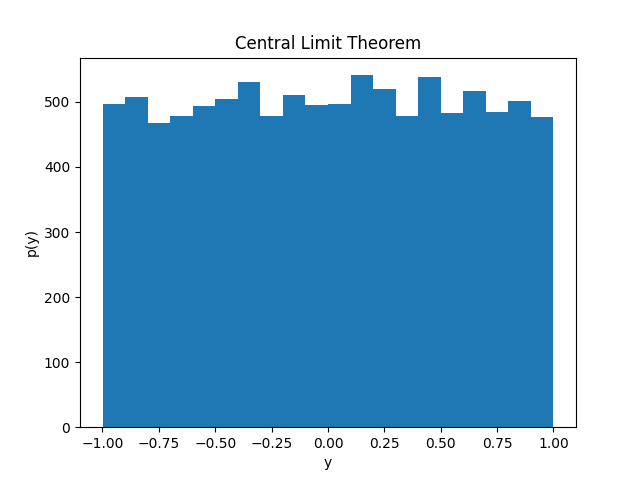
\includegraphics[width=2in]{images/central1.png} &
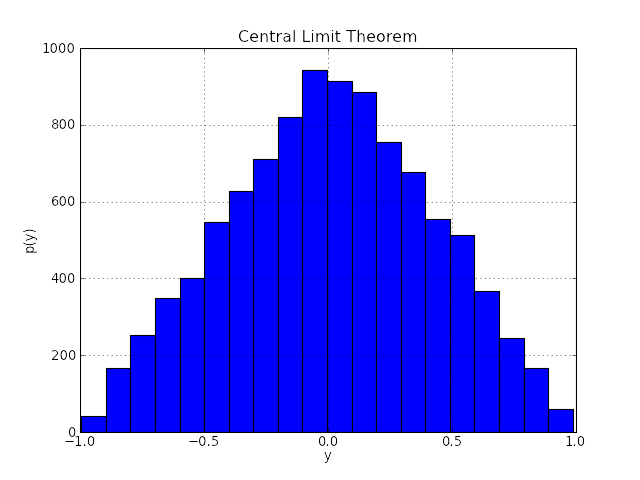
\includegraphics[width=2in]{images/central2.png} \\
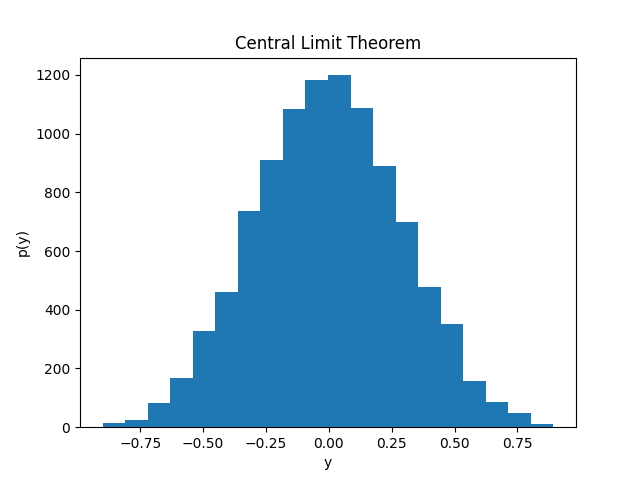
\includegraphics[width=2in]{images/central4.png} &
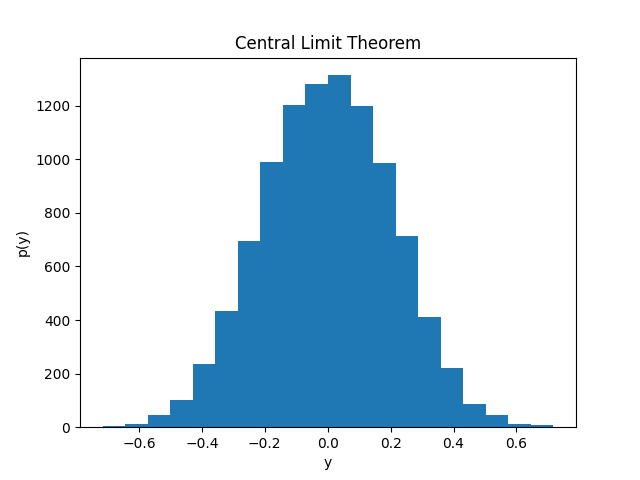
\includegraphics[width=2in]{images/central8.png}
\end{tabular}
\end{center}
\caption{Example of distributions for sums of 1, 2, 4, and 8 uniform random variables. The more random variables are added, the better the result approximates a Gaussian distribution.\label{central}}
\end{figure}

This theorem is of fundamental importance for stochastic calculus. Notice that the theorem does not apply when the $X_i$ follow distributions that do not have a finite mean or a finite variance.

\index{Levy distributions}

Distributions that do not follow the central limit are called {\it Levy distributions}.
They are characterized by fat tails for the form

\begin{equation}
p(x) \stackunder{x\rightarrow\infty}{\sim} \frac1{\left|x\right|^{1+\alpha}}, \qquad 0<\alpha<2
\end{equation}

An example is the Pareto distribution.

\goodbreak\subsection{Error in the mean}
\index{error in the mean}

One consequence of the Central Limit Theorem is a useful formula for evaluating the error in the mean.
Let"s consider the case of $N$ repeated experiments with outcomes $X_i$.
Let"s also assume that each $X_i$ is supposed to be equal to an unknown
value $\mu $, but in practice, $X_i=\mu +\varepsilon $, where $\varepsilon $ is
a random variable with Gaussian distribution centered at zero. One could
estimate $\mu $ by $\mu =E[X]=\frac 1N\Sigma _iX_i$.
In this case, statistical error in the mean is given by
\begin{equation}
\delta \mu =\sqrt{\frac{\sigma ^2}{N}}
\label{error}
\end{equation}
where $\sigma ^2=E[(X-\mu )^2]=\frac 1N\Sigma _i(X_i-\mu )^2$.



\goodbreak\section{Combinatorics and discrete random variables}
\index{combinatorics}

Often, to compute the probability of discrete random variables, one
has to confront the problem of calculating the number of possible finite
outcomes of an experiment. Often this problem is solved by combinatorics.

\goodbreak\subsection{Different plugs in different sockets}

If we have $n$ different plugs and $m$ different sockets; in how many ways
can we place the plugs in the sockets?

\begin{itemize}
\item  Case 1, $n\geq m$. All sockets will be filled. We consider the first
socket, and we can select any of the $n$ plugs ($n$ combinations). We
consider the second socket, and we can select any of the remaining $n-1$
plugs ($n-1$ combinations), and so on, until we are left with no free sockets
and $n-m$ unused plugs; therefore there are
\begin{equation}
n!/(n-m)!=n(n-1)(n-2)...(n-m+1)
\end{equation}
combinations.

\item  Case 2, $n\leq m$. All plugs have to be used. We consider the first
plug, and we can select any of the $m$ sockets ($m$ combinations). We
consider the second plug, and we can select any of the remaining $m-1$
sockets ($m-1$ combinations), and so on, until we are left with no spare
plugs and $m-n$ free sockets; therefore there are
\begin{equation}
m!/(m-n)!=m(m-1)(m-2)...(m-n+1)
\end{equation}
combinations. Note that if $m=n\, $ then case 1 and case 2 agree, as
expected.
\end{itemize}

\goodbreak\subsection{Equivalent plugs in different sockets}

If we have $n$ equivalent plugs and $m$ different sockets, in how many ways
can we place the plugs in the sockets?

\begin{itemize}
\item  Case 1, $n\geq m$. All sockets will be filled. We cannot distinguish
one combination from the other because all plugs are the same. There is only
one combination.

\item  Case 2, $n\leq m$. All plugs have to be used but not all sockets.
There are $m!/(m-n)!$ ways to fill the sockets with different plugs, and
there are $n!$ ways to arrange the plugs within the same filled sockets.
Therefore there are
\begin{equation}
\binom mn=\frac{m!}{(m-n)!n!}
\end{equation}
ways to place $n$ equivalent plugs into $m$ different sockets. Note that if $%
m=n$%
\begin{equation}
\binom nn=\frac{n!}{(n-n)!n!}=1
\end{equation}
in agreement with case 1.
\end{itemize}

Here is another example. A club has 20 members and has to elect a president, a vice president, 
a secretary, and a treasurer. In how many different ways can they select the
four officeholders? Think of each office as a socket and each person as a
plug; therefore the number combination is $20!/(20-4)!\simeq \allowbreak
1.\, 2\times 10^5$.

\goodbreak\subsection{Colored cards}

We have 52 cards, 26 black and 26 red. We shuffle the cards and pick three.

\begin{itemize}
\item  What is the probability that they are all red?
\begin{equation}
\textrm{Prob}(3red)=\frac{26}{52}\times \frac{25}{51}\times \frac{24}{50}=\frac{2}{17}
\end{equation}

\item  What is the probability that they are all black?
\begin{equation}
\textrm{Prob}(3black)=\textrm{Prob}(3red)=\frac{2}{17}
\end{equation}

\item  What is the probability that they are not all black or all red?
\begin{eqnarray}
\textrm{Prob}(mixture) &=&1-\textrm{Prob}(3red\cup 3black) \\
&=&1-\textrm{Prob}(3red)-\textrm{Prob}(3black) \\
&=&1-2\frac{2}{17} \\
&=&\frac{13}{17}
\end{eqnarray}
\end{itemize}

Here is an example of how we can simulate the deck of cards to compute an answer to the last question:

\begin{lstlisting}
proc makeDeck(): seq[string] =
  for i in 0 ..< 26:
    result.add "red"
    result.add "black"

proc makeShuffledDeck(): seq[string] =
  result = makeDeck()
  shuffle(result)

proc pickThreeCards(): seq[string] = makeShuffledDeck()[0 ..< 3]

proc simulateCards(n = 1000): float =
  var counter = 0
  for _ in 0 ..< n:
    let c = pickThreeCards()
    if not (c[0] == c[1] and c[1] == c[2]):
      counter += 1
  result = counter / n

echo simulateCards()
\end{lstlisting}

\goodbreak\subsection{Gambler"s fallacy}

The typical error in computing probabilities is mixing a priori probability
with information about past events.
This error is called the {\it gambler"s fallacy}~\cite{gambler}.
For example, we consider the preceding problem. We see the first two cards, and they are both red. What is the
probability that the third one is also red?

\begin{itemize}
\item  {\bf Wrong answer}: The probability that they are all red is $%
\textrm{Prob}(3red)=2/17$; therefore the probability that the third one is also $2/17$.

\item  {\bf Correct answer}: Because we know that the first two cards are red, the third card must belong to a set of (26 black cards + 24 red cards);
therefore the probability that it is red is
\begin{equation}
\textrm{Prob}(red)=\frac{24}{24+26}=\frac{12}{25}
\end{equation}
\end{itemize}




\chapter{Random Numbers and Distributions}

In the previous chapters, we have seen how using the {\ft std/random} module, we can generate uniform random numbers. This module can also
generate random numbers following other distributions.
The point of this chapter is to understand how random numbers are generated.

\goodbreak\section{Randomness, determinism, chaos and order}
\index{randomness}\index{determinism}\index{chaos}\index{order}

Before we proceed further, there are four important concepts that should be defined because of their implications:

\begin{itemize}
\item  {\bf Randomness} is the characteristic of a process whose outcome is
unpredictable (e.g., at the moment I am writing this sentence, I cannot
predict the exact time and date when you will be reading it).

\item  {\bf Determinism} is the characteristic of a process whose outcome
can be predicted from the initial conditions of the system (e.g., if I throw a
ball from a known position, at a known velocity and in a known direction, I
can predict---calculate---its entire future trajectory).

\item  {\bf Chaos} is the emergence of randomness from order~\cite{lorenz}
(e.g., if I am on the
top of a hill and I throw the ball in a vertical direction, I cannot predict on
which side of the hill it is going to end up). Even if the equations that
describe a phenomenon are known and are deterministic, it may happen that a
small variation in the initial conditions causes a large difference in the
possible deterministic evolution of the system. Therefore the outcome of a
process may depend on a tiny variation of the initial parameters. These
variations may not be measurable in practice, thus making the process
unpredictable and chaotic. Chaos is generally regarded as a characteristic
of some differential equations.

\item  {\bf Order} is the opposite of chaos. It is the emergence of regular
and reproducible patterns from a process that, in itself, may be random or
chaotic (e.g., if I keep throwing my ball in a vertical direction from
the top of a hill and I record the final location of the ball, I eventually
find a regular pattern, a probability distribution associated with my
experiment, which depends on the direction of the wind, the shape of the
hill, my bias in throwing the ball, etc.).
\end{itemize}

These four concepts are closely related, and they do not necessarily come in
opposite pairs as one would expect.

A deterministic process may cause chaos. We can use chaos to generate
randomness (we will see examples when covering random number generation). We
can study randomness and extract its ordered properties (probability
distributions), and we can use randomness to solve deterministic problems
(Monte Carlo) such as computing integrals and simulating a system.

\goodbreak\section{Real randomness}
\index{radioactive decay}

Note that randomness does not necessarily come from chaos.
Randomness exists in nature~\cite{determinism}\cite{decay}.
For example, a radioactive atom ``decays'' into a different atom
at some random point in time. For example, an atom of carbon 14 decays into nitrogen 14 by emitting an electron and a neutrino
\begin{equation}
_6^{14}C\longrightarrow _7^{14}N+e^{-}+\overline{\nu }_e
\end{equation}
at some random time $t$; $t$ is unpredictable. It can be proven that the
randomness in the nuclear decay time is not due to any underlying
deterministic process. In fact, constituents of matter are
described by quantum physics, and randomness is a fundamental characteristic
of quantum systems. Randomness is not a consequence of our ignorance.

This is not usually the case for macroscopic systems. Typically the
randomness we observe in some macroscopic systems is not always a
consequence of microscopic randomness. Rather, order and determinism
emerge from the microscopic randomness, while chaos originates from the complexity of
the system.

Because randomness exists in nature, we can use it to produce random numbers
with any desired distribution. In particular, we want to use the randomness
in the decay time of radioactive atoms to produce random numbers with
uniform distribution. We assemble a system consisting of many
atoms, and we record the time when we observe atoms decay:

\begin{equation}
t_0, t_1, t_2, t_3, t_4, t_5, ...
\end{equation}

One could study the probability distribution of the $t_i$ and find
that it follows an exponential probability distribution like

\begin{equation}
\textrm{Prob}(t_i = t)=\lambda e^{-\lambda t}
\end{equation}

where $t_0=1/\lambda $ is the decay time characteristic of the particular
type of atom. One characteristic of this distribution is that it is a memoryless process: $t_i$ does not depend on $t_{i-1}$ and therefore the probability that $t_i>t_{i-1}$ is the same as the probability that $t_i<t_{i-1}$.

\goodbreak\subsection{Memoryless to Bernoulli distribution}

\index{distribution!memoryless}
\index{distribution!Bernoulli}

Given the sequence $\{t_i\}$ with exponential distribution, we can build a
random sequence of zeros and ones (Bernoulli distribution) by applying the following formula, known as the Von Neumann procedure~\cite{bits}:
\begin{equation}
x_i=\left\{
\begin{array}{ll}
1 & \text{if }t_{i}>t_{i-1} \\
0 & \text{otherwise}
\end{array}
\right.
\end{equation}

Note that the procedure can be applied to map any random sequence into
a Bernoulli sequence even if the numbers in the original sequence do not
follow an exponential distribution, as long as $t_i$ is independent of $t_j$
for any $j<i$ (memoryless distribution).

\goodbreak\subsection{Bernoulli to uniform distribution}

\index{distribution!uniform}

To map a Bernoulli distribution into a uniform distribution, we need
to determine the precision (resolution in number of bits) of the numbers we wish
to generate. In this example, we will assume 8 bits.

We can think of each number as a point in a [0, 1) segment. We generate the
uniform number by making a number of choices: we break the segment in two
and, according to the value of the binary digit (0 or 1), we select the first
part or the second part and repeat the process on the subsegment. Because
at each stage we break the segment into two parts of equal length and we
select one or the other with the same probability, the final distribution of
the selected point is uniform. As an example, we consider the Bernoulli
sequence
\begin{equation}
01011110110101010111011010
\end{equation}
and we perform the following steps:

\begin{itemize}
\item  break the sequence into chunks of 8 bits
\begin{equation}
\text{01011110-11010101-01110110-.....}
\end{equation}

\item  map each chunk $a_0a_1a_2a_3a_4a_5a_6a_7$ into $x=\sum_{k=0}^{k<8}a_k/2^{k+1}$
thus obtaining:

\begin{equation}
0.3671875 - 0.83203125 - 0.4609375 - ...
\end{equation}
\end{itemize}

A uniform random number generator is usually the first step toward building
any other random number generator.

\index{entropy source}

Other physical processes can be used to generate real random numbers using a similar process.
Some microprocessors can generate random numbers from random temperature fluctuations.
An unpredictable source of randomness is called an {\it entropy source}.

\goodbreak\section{Entropy generators}

The Linux/Unix operating system provides its own entropy source accessible via {\ft /dev/urandom}. From Nim, we read it as a regular file using {\ft std/streams}.

Here we define a class that can access this entropy source and use it to generate uniform random numbers. It follows the same process outlined for the radioactive days:

\index{class!URANDOM}

\begin{lstlisting}
import std/[os, streams]

type URANDOM* = ref object

proc newURANDOM*(data = ""): URANDOM =
  result = URANDOM()
  if data.len > 0:
    let s = newFileStream("/dev/urandom", fmWrite)
    if not s.isNil:
      s.write(data); s.close()

proc random*(u: URANDOM): float =
  const n = 16
  var bytes = newString(n)
  let s = newFileStream("/dev/urandom", fmRead)
  doAssert s.readData(addr bytes[0], n) == n
  s.close()
  var randomInteger = 0'u64
  for k in 0 ..< n:
    randomInteger += uint64(byte(bytes[k])) * (256'u64 ^ k)
  result = float(randomInteger) / (256.0 ^ n)
\end{lstlisting}

Notice how the constructor allows us to further randomize the data by contributing input to the entropy source. Also notice how the {\ft random()} method reads 16 bytes from the stream (using {\ft os.urandom()}), converts each into $8$-bit integers, combines them into a $128$-bit integer, and then converts it to a float by dividing by $256^{16}$.

\goodbreak\section{Pseudo-randomness}

In many cases we do not have a physical device to generate random numbers, 
and we require a software solution. Software is deterministic, the outcome
is reproducible, therefore it cannot be used to generate randomness, but it
can generate pseudo-randomness. The outputs of pseudo random number
generators are not random, yet they may be considered random for practical purposes.
John von Neumann observed in 1951 that ``anyone who
considers arithmetical methods of producing random digits is, of course, in
a state of sin.'' (For attempts to generate ``truly random'' numbers, see
the article on hardware random number generators.) Nevertheless, 
pseudo random numbers are a critical part of modern computing, from
cryptography to the Monte Carlo method for simulating physical systems.

Pseudo random numbers are relatively easy to generate with software, and they
provide a practical alternative to random numbers. For some applications, 
this is adequate.



\goodbreak\subsection{Linear congruential generator}

Here is probably the simplest possible pseudo random number generator:

\begin{eqnarray}
x_i &=&(a x_{i-1} + c) \textrm{mod}m \\
y_i &=&x_i/m
\end{eqnarray}
With the choice $a=65539$, $c=0$, and $m=2^{31}$, this generator is called RANDU. It is of historical importance
because it is implemented in the C {\ft rand()} function.
The RANDU generator is particularly fast because the modulus can
be implemented using the finite 32-bit precision.

Here is a possible implementation for $c=0$:
%%% META:FILE:nlib/randomgen.nim
\begin{lstlisting}[caption={in file: {\ft nlib/randomgen.nim}}]
type
  MCG* = ref object
    x*, a*, m*: int

proc newMCG*(seed: int, a = 66539, m = 1 shl 31): MCG =
  MCG(x: seed, a: a, m: m)

proc next*(g: MCG): int =
  g.x = (g.a * g.x) mod g.m
  g.x

proc random*(g: MCG): float =
  float(g.next()) / float(g.m)
\end{lstlisting}

which we can test with
\begin{lstlisting}
let randu = newMCG(seed = 1071914055)
for i in 0 ..< 10: echo randu.random()
\end{lstlisting}

The output numbers ``look'' random but are not truly random. Running the same code with the same seed generates the same output. Notice the following:

\begin{itemize}
\item  PRNGs are typically implemented as a recursive expression that, given $%
x_{i-1}$, produces $x_i$.

\index{seed}


\item  PRNGs have to start from an initial value, $x_0$, called the {\it seed}.
A typical choice is to set the seed equal to the number of seconds from the
conventional date and time ``Thu Jan 01 01:00:00 1970.'' This is not always
a good choice.

\item PRNGs are periodic. They generate numbers in a finite set and then they repeat themselves. It is desirable to have this set as large as possible.

\item  PRNGs depend on some parameters (e.g., $a$ and $m$). Some
parameter choices lead to trivial random number generators. In
general, some choices are better than others, and a few are optimal. In
particular, the values of $a$ and $m$ determine the period of the random
number generator. An optimal choice is the one with the longest period.
\end{itemize}

For a linear congruential generator, because of the {\ft mod} operation, the period is always less than or equal to $m$. When $c$ is nonzero, the period is equal to $m$ only if $c$ and $m$ are relatively prime, $a-1$ is divisible by all prime factors of $m$, and $a-1$ is a multiple of 4 when $m$ is a multiple of $4$.

In the case of RANDU, the period is $m/4$. A better choice is using $a=7^5$ and $m=2^{31}-1$ (known as the Marsenne prime number) because it can be proven that $m$ is in fact the period of the generator:
\begin{equation}
x_i=(7^5x_{i-1})\textrm{mod}(2^{31}-1)  \label{Marsenne}
\end{equation}

Here are some examples of MCG used by various systems:

\begin{tabular}{|lrrr|} \hline
Source & $m$ & $a$ & $c$ \\ \hline
Numerical Recipes & $2^{32}$ & 1664525 & 1013904223 \\
glibc (used by GCC) & $2^{32}$ & 1103515245 & 12345 \\
Apple CarbonLib & $2^{31} - 1$ & 16807 & 0 \\
java.util.Random & $2^{48}$ & 25214903917 & 11 \\ \hline
\end{tabular}

When $c$ is set to zero, a linear congruential generator is also called a multiplicative congruential generator.

\goodbreak\subsection{Defects of PRNGs}

The non-randomness of pseudo random number generators manifests itself in at
least two different ways:

\begin{itemize}
\item  The sequence of generated numbers is periodic, therefore only a finite
set of numbers can come out of the generator, and many of the numbers will never be
generated. This is not a major problem if the period is much larger (some
order of magnitude) than the number of random numbers needed in the Monte
Carlo computation.

\item  The sequence of generated numbers presents bias in the form of
``patterns.'' Sometimes
these patterns are evident, sometimes they are not evident. Patterns exist
because the pseudo random numbers are not random but are generated using a
recursive formula. The existence of these patterns may introduce a bias in
Monte Carlo computations that use the generator. This is a nasty problem, and
the implications depend on the specific case.
\end{itemize}

An example of pattern/bias is discussed in ref.~\cite{randu} and can be seen in fig.~\ref{randu}.

\begin{figure}[ht]
  \centering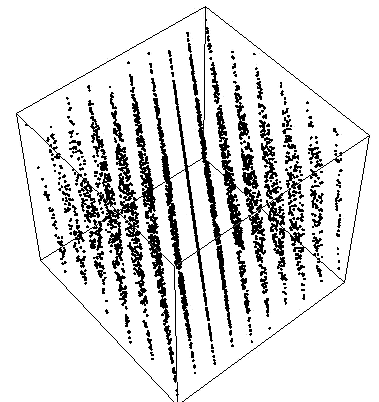
\includegraphics[width=2.5in]{images/randu.png}
\caption{In this plot, each three consecutive random numbers (from RANDU) are interpreted as $(x, y, z)$ coordinates of a random point. The image clearly shows the points are not distributed at random. Image from ref.~\cite{randu}.\label{randu}}
\end{figure}

\goodbreak\subsection{Multiplicative recursive generator}

Another modification of the multiplicative congruential generator is the following:

\begin{equation}
x_i=(a_1x_{i-1}+a_2x_{i-2}+...+a_kx_{i-k})\textrm{mod}m
\end{equation}

The advantage of this generator is that if $m$ is prime, the period of this
type of generator can be as big as $m^k-1$. This is much larger than a
simple multiplicative congruential generator.

An example is $a_1=107374182, $ $a_2=a_3=a_4=0, $ $a_5=104480$, and $m=2^{31}-1$, 
where the period is
\begin{equation}
(2^{31}-1)^5-1\simeq 4.56\times 10^{46}
\end{equation}

\goodbreak\subsection{Lagged Fibonacci generator}

\begin{equation}
x_i=(x_{i-j}+x_{i-k})\textrm{mod}m
\end{equation}

This is similar to the multiplicative recursive generator earlier. If $m$ is
prime and $j\neq k$, the period can be as large as $m^k-1$.

\goodbreak\subsection{Marsaglia"s add-with-carry generator}

\begin{equation}
x_i=(x_{i-j}+x_{i-k}+c_i)\textrm{mod}m
\end{equation}

where $c_1=0$ and $c_i=1$ if $(x_{i-1-j}+x_{i-1-k}+c_{i-1})<m$, $0$

\goodbreak\subsection{Marsaglia"s subtract-and-borrow generator}

\begin{equation}
x_i=(x_{i-j}-x_{i-k}-c_i)\textrm{mod}m
\end{equation}

where $k>j>0$, $c_1=0$, and $c_i=1$ if $(x_{i-1-j}-x_{i-1-k}-c_{i-1})<0$, $0$
otherwise.

\goodbreak\subsection{L\"uscher"s generator}

The Marsaglia"s subtract-and-borrow is a very popular generator, but it is known
to have some problems. For example, if we construct vector
\begin{equation}
v_i=(x_i, x_{i+1}, ..., x_{i+k})
\end{equation}
and the coordinates of the point $v_i$ are numbers closer to each other then
the coordinates of the point $v_{i+k}$ are also close to each other. This
indicates that there is an unwanted correlation between the points $%
x_i, x_{i+1}, ..., x_{i+k}$. L\"uscher observed~\cite{lusher} that the Marsaglia"s
subtract-and-borrow is equivalent to a chaotic discrete dynamic system, and
the preceding correlation dies off for points that distance themselves more than $k$. Therefore
he proposed to modify the generator as follows: instead of taking all $x_i$
numbers, read $k$ successive elements of the sequence, discard $p-k$
numbers, read $k$ numbers, and so on. The number $p$ has to be chosen to be
larger than $k$. When $p=k$, the original Marsaglia generator is recovered.

\goodbreak\subsection{Knuth"s polynomial congruential generator}

\begin{equation}
x_i=(ax_{i-1}^2+bx_{i-1}+c)\textrm{mod}m
\end{equation}

This generator takes the form of a more complex function. It makes it harder to guess one number in the sequence from the following numbers; therefore
it finds applications in cryptography.

Another example is the Blum, Blum, and Shub generator:
\begin{equation}
x_i=x_{i-1}^2\textrm{mod}m
\end{equation}

\goodbreak\subsection{PRNGs in cryptography}

Random numbers find many applications in cryptography. For example, consider
the problem of generating a random password, a digital signature, or random
encryption keys for the Diffie--Hellmann and the RSA encryption schemes.

A cryptographically secure pseudo random number generator (CSPRNG) is a
pseudo random number generator (PRNG) with properties that make it suitable
for use in cryptography.

In addition to the normal requirements for a PRNG (that its output
should pass all statistical tests for randomness) a CSPRNG must have two
additional properties:

\begin{itemize}
\item  It should be difficult to predict the output of the CSPRNG, wholly or
partially, from examining previous outputs.

\item  It should be difficult to extract all or part of the internal state
of the CSPRNG from examining its output.
\end{itemize}

Most PRNGs are not suitable for use as CSPRNGs. They must appear random
in statistical tests, but they are not designed to resist determined
mathematical reverse engineering.

CSPRNGs are designed explicitly to resist reverse engineering. There are a
number of examples of CSPRNGs. Blum, Blum, and Shub has the strongest security
proofs, though it is slow.

Many pseudo random number generators have the form
\begin{equation}
x_i=f(x_{i-1}, x_{i-2}, ..., x_{i-k})
\end{equation}
For example, the next random number depends on the past $k$ numbers. Requirements for CSPRNGs used in cryptography are that

\begin{itemize}
\item  Given $x_{i-1}, x_{i-2}, ..., x_{i-k}$, $x_i$ can be computed in
polynomial time, while

\item  Given $x_i, x_{i-2}, ..., x_{i-k}$, $x_{i-1}$ must not be computable in
polynomial time.
\end{itemize}

The first requirement means that the PRNG must be fast. The second
requirement means that if a malicious agent discovers a random number used
as a key, he or she cannot easily compute all previous keys generated using the
same PRNG.

\goodbreak\subsection{Inverse congruential generator}

\begin{equation}
x_i=(ax_{i-1}^{-1}+c)\textrm{mod}m
\end{equation}

where $x_{i-1}^{-1}$ is the multiplicative inverse of $x_{i-1}$ modulo $m$, 
for example, $x_{i-1}x_{i-1}^{-1}=1\textrm{mod}m$.


\goodbreak\subsection{Marsenne twister}

One of the best PRNG algorithms (because of its long period, uniform distribution, and speed) is the Marsenne twister, which produces a 53-bit random number, 
and it has a period of $2^{19937}-1$ (this number is 6002 digits long!).
Nim's {\ft std/random} module is built on top of a Mersenne-twister-style generator (specifically Xoshiro/Mersenne, depending on the implementation).
Although discussing the inner working of this algorithm is beyond the scope of these notes, we provide a
pure-Nim implementation of the Marsenne twister:

\index{class!MarsenneTwister}

%%% META:FILE:nlib/randomgen.nim
\begin{lstlisting}[caption={in file: {\ft nlib/randomgen.nim}}]
type
  MarsenneTwister* = ref object
    w*: array[625, uint32]
    wi*: int

proc newMarsenneTwister*(seed: uint32 = 4357'u32): MarsenneTwister =
  result = MarsenneTwister()
  result.w[0] = seed
  for i in 1 ..< 625:
    result.w[i] = 69069'u32 * result.w[i-1]
  result.wi = 624

proc random*(g: MarsenneTwister): float =
  const
    N = 624
    M = 397
    U = 0x80000000'u32
    L = 0x7fffffff'u32
  let K = [0'u32, 0x9908b0df'u32]
  var y: uint32 = 0
  if g.wi >= N:
    var kk = 0
    while kk < N - M:
      y = (g.w[kk] and U) or (g.w[kk + 1] and L)
      g.w[kk] = g.w[kk + M] xor (y shr 1) xor K[y and 1'u32]
      inc kk
    while kk < N - 1:
      y = (g.w[kk] and U) or (g.w[kk + 1] and L)
      g.w[kk] = g.w[kk + (M - N)] xor (y shr 1) xor K[y and 1'u32]
      inc kk
    y = (g.w[N - 1] and U) or (g.w[0] and L)
    g.w[N - 1] = g.w[M - 1] xor (y shr 1) xor K[y and 1'u32]
    g.wi = 0
  y = g.w[g.wi]; inc g.wi
  y = y xor (y shr 11)
  y = y xor ((y shl 7) and 0x9d2c5680'u32)
  y = y xor ((y shl 15) and 0xefc60000'u32)
  y = y xor (y shr 18)
  result = float(y) / float(0xffffffff'u32)
\end{lstlisting}

In the above code, numbers starting with \verb!0x! are represented in hexadecimal notation, and the {\ft 'u32} suffix fixes their type as unsigned 32-bit integers. The keywords {\ft and}, {\ft or}, {\ft xor}, {\ft shl}, and {\ft shr} are Nim's bitwise operators (when applied to integer types): {\ft and} is binary AND, {\ft xor} is binary exclusive OR, {\ft shl} shifts all bits to the left, and {\ft shr} shifts all bits to the right. The Nim manual gives the full details.

\goodbreak\section{Parallel generators and independent sequences}

It is often necessary to generate many independent sequences.

For example, you may want to generate streams or random numbers in parallel using multiple machines and processes, and you need to ensure that the streams do not overlap.

A common mistake is to generate the sequences using the same
generator with different seeds. This is not a safe procedure because it is
not obvious if the seed used to generate one sequence belongs to the
sequence generated by the other seed. The two
sequences of random numbers are not independent, but they are merely
shifted in respect to each other.

For example, here are two RANDU sequences generated with different but dependent
seeds:
\begin{equation}
\begin{tabular}{lll}
seed & 1071931562 & 50554362 \\
$y_0$ & 0.252659081481 & 0.867315522395 \\
$y_1$ & 0.0235412092879 & 0.992022250779 \\
$y_2$ & 0.867315522395 & 0.146293803118 \\
$y_3$ & 0.992022250779 & 0.949562561698 \\
$y_4$ & 0.146293803118 & 0.380731142126 \\
$y_5$ & ... & ...
\end{tabular}
\end{equation}

Note that the second sequence is the same as the first but shifted by two
lines.

Three standard techniques for generating independent sequences are
non-overlapping blocks, leapfrogging, and Lehmer trees.

\goodbreak\subsection{Non-overlapping blocks}

Let"s consider one sequence of pseudo random numbers:
\begin{equation}
x_0, x_1, ..., x_k, x_{k+1}, ..., x_{2k}, x_{2k+1}, ..., x_{3k}, x_{3k+1}, ..., 
\end{equation}
One can break it into subsequences of $k$ numbers:
\begin{eqnarray}
&&x_0, x_1, ..., x_{k-1} \\
&&x_k, x_{k+1}, ..., x_{2k-1} \\
&&x_{2k}, x_{2k+1}, ..., x_{3k-1} \\
&&...
\end{eqnarray}
If the original sequence is created with a multiplicative congruential
generator
\begin{equation}
x_i=ax_{i-1}\textrm{mod}m
\end{equation}
the subsequences can be generated independently because
\begin{equation}
x_{nk-1}=a^{nk-1}x_0\textrm{mod}m
\end{equation}
if the seed of the arbitrary sequence is $x_{nk}, x_{nk+1}, ..., x_{nk-1}$. This
is particularly convenient for parallel computers where one computer
generates the seeds for the subsequences and the processing nodes, 
independently, generated the subsequences.

\goodbreak\subsection{Leapfrogging}

Another and probably more popular technique is leapfrogging.
Let"s consider one sequence of pseudo random numbers:
\begin{equation}
x_0, x_1, ..., x_k, x_{k+1}, ..., x_{2k}, x_{2k+1}, ..., x_{3k}, x_{3k+1}, ..., 
\end{equation}
One can break it into subsequences of $k$ numbers:
\begin{eqnarray}
&&x_0, x_k, x_{2k}, x_{3k}, ... \\
&&x_1, x_{1+k}, x_{1+2k}, x_{1+3k}, ... \\
&&x_2, x_{2+k}, x_{2+2k}, x_{2+3k}, ... \\
&&...
\end{eqnarray}

The seeds $x_1, x_2, ..x_{k-1}$ are generated from $x_0$, and the independent
sequences can be generated independently using the formula
\begin{equation}
x_{i+k}=a^kx_i\textrm{mod}m
\end{equation}
Therefore leapfrogging is a viable technique for parallel random number
generators.

Here is an example of a usage of {\ft leapfrog}:

%%% META:FILE:nlib/randomgen.nim
\begin{lstlisting}[caption={in file: {\ft nlib/randomgen.nim}}]
proc leapfrog*(mcg: MCG, k: int): seq[MCG] =
  # Compute (mcg.a^k) mod mcg.m incrementally to avoid integer
  # overflow: for typical seeds, mcg.a^k overflows int64 long before
  # `k` reaches a useful number of streams.
  var a = 1
  for _ in 0 ..< k:
    a = (a * mcg.a) mod mcg.m
  for i in 0 ..< k:
    result.add newMCG(mcg.next(), a, mcg.m)
\end{lstlisting}

Here is an example of usage:
\begin{lstlisting}
let generators = leapfrog(newMCG(m), 3)
for k in 0 ..< 3:
  for i in 0 ..< 5:
    let x = generators[k].random()
    echo k, "\t", i, "\t", x
\end{lstlisting}

The Marsenne twister algorithm implemented in {\ft os.random} has leapfrogging built in. In fact, the module includes a {\ft random.jumpahead(n)} method that allows us to efficiently skip $n$ numbers.

\goodbreak\subsection{Lehmer trees}

Lehmer trees are binary trees, generated recursively, where each node
contains a random number. We start from the root containing the seed, $x_0$, and
we append two children containing, respectively, 
\begin{eqnarray}
x_i^L &=&(a_Lx_{i-1}+c_L)\textrm{mod}m \\
x_i^R &=&(a_Rx_{i-1}+c_R)\textrm{mod}m
\end{eqnarray}
then, recursively, append nodes to the children.

\goodbreak\section{Generating random numbers from a given distribution}

\index{accept-reject}\index{inversion method}

In this section and the next, we provide examples of distributions other than uniform and algorithms to generate numbers using these distributions. The general strategy consists of finding ways to map uniform random numbers into numbers following a different distribution. There are two general techniques for mapping uniform into nonuniform random numbers:

\begin{itemize}
\item accept--reject (applies to both discrete and continuous distributions)
\item inversion methods (applies to continuous distributions only)
\end{itemize}

Consider the problem of generating a random number $x$ from a given distribution $p(x)$. The {\it accept--reject method} consists of generating $x$ using a different distribution, $g(x)$, and a uniform random number, $u$, between 0, 1. If $u<p(x)/Mg(x)$ ($M$ is the max of $p(x)/g(x)$), then $x$ is the desired random number following distribution $p(x)$. If not, try another number.

To visualize why this works, imagine graphing the distribution $p$ of the random variable $x$ onto a large rectangular board and throwing darts at it, the coordinates of the dart being $(x, u)$. Assume that the darts are uniformly distributed around the board. Now take off (reject) all of the darts that are outside the curve. The remaining darts will be distributed uniformly within the curve, and the $x$-positions of these darts will be distributed according to the random variable"s density. This is because there is the most room for the darts to land where the curve is highest and thus the probability density is greatest.

The $g$ distribution is nothing but a shape so that all darts we throw are below it. There are two particular cases. In one case, $g=p$, we only throw darts below the $p$ that we want; therefore we accept them all. This is the most efficient case, but it is not of practical interest because it means the accept--reject is not doing anything, as we already know now to generate numbers according to $p$. The other case is $g(x) = constant$. This means we generate the $x$ uniformly before the accept--reject. This is equivalent to throwing the darts everywhere on the square board, without even trying to be below the curve $p$.

The inversion method instead is more efficient but requires some math. It states that if $F(x)$ is a cumulative distribution function and $u$ is a uniform random number between 0 and 1, then $x = F^{-1}(u)$ is a random number with distribution $p(x)=f'(x)$. For those distributions where $F$ can be expressed in analytical terms and inverted, the inversion method is the best way to generate random numbers. An example is the exponential distribution.

We will create a new class {\ft RandomSource} that includes methods to generate the random number.

\goodbreak\subsection{Uniform distribution}

The uniform distributions are simple probability distributions which, in the
discrete case, can be characterized by saying that all possible values are
equally probable. In the continuous case, one says that all intervals of the
same length are equally probable.

There are two types of uniform distribution: discrete and continuous.

Here we consider the discrete case as we implement it into a {\ft randint} method:

\index{class!RandomSource}

%%% META:FILE:nlib/randomgen.nim
\begin{lstlisting}[caption={in file: {\ft nlib/randomgen.nim}}]
type
  RandomSource* = ref object
    generator*: proc(): float    # any uniform `[0, 1)` source

proc newRandomSource*(generator: proc(): float = nil): RandomSource =
  let g = if generator.isNil: (proc(): float = rand(1.0)) else: generator
  RandomSource(generator: g)

proc random*(r: RandomSource): float = r.generator()

proc randint*(r: RandomSource, a, b: int): int =
  a + int(float(b - a + 1) * r.random())
\end{lstlisting}

Notice that the random {\ft RandomSource} constructor expects a generator such as {\ft MCG}, {\ft MarsenneTwister}, or simply {\ft random} (default value). The {\ft random()} method is a proxy method for the equivalent method of the underlying generator object.

We can use {\ft randint} to generate a random choice from a finite set when each option has the same probability:

%%% META:FILE:nlib/randomgen.nim
\begin{lstlisting}[caption={in file: {\ft nlib/randomgen.nim}}]
proc choice*[T](r: RandomSource, S: openArray[T]): T =
  S[r.randint(0, S.len - 1)]
\end{lstlisting}

\goodbreak\subsection{Bernoulli distribution}

The Bernoulli distribution, named after Swiss scientist James Bernoulli, is
a discrete probability distribution that takes value 1 with
probability of success $p$ and value 0 with probability of failure $q=1-p$:

\begin{equation}
p(k) \equiv \left\{
\begin{array}{ll}
p & \text{if }k=1 \\
1-p & \text{if }k=0 \\
0 & \text{if not }k \in \{0, 1\}
\end{array}
\right\}
\end{equation}
A Bernoulli random variable has an expected value of $p$ and variance of $pq$.

We implement it by adding a corresponding method to the {\ft RandomSource} class:

%%% META:FILE:nlib/randomgen.nim
\begin{lstlisting}[caption={in file: {\ft nlib/randomgen.nim}}]
proc bernoulli*(r: RandomSource, p: float): int =
  if r.random() < p: 1 else: 0
\end{lstlisting}

\goodbreak\subsection{Biased dice and table lookup}

A generalization of the Bernoulli distribution is a distribution in which we have a finite set of choices, each with an associated probability. The table can be a list of tuples {\ft (value, probability)} or a dictionary of {\ft value:probability}:

%%% META:FILE:nlib/randomgen.nim
\begin{lstlisting}[caption={in file: {\ft nlib/randomgen.nim}}]
proc lookup*[K](r: RandomSource, table: seq[(K, float)],
                epsilon = 1e-6): K =
  var u = r.random()
  for (key, p) in table:
    if u < p + epsilon: return key
    u = u - p
  raise newException(ArithmeticDefect, "invalid probability")
\end{lstlisting}

Let"s say we want a random number generator that can only produce the
outcome 0, 1 or 2 with known probabilities:
\begin{eqnarray}
\textrm{Prob}(X &=&0)=0.50 \\
\textrm{Prob}(X &=&1)=0.23 \\
\textrm{Prob}(X &=&2)=0.27
\end{eqnarray}
Because the probability of the possible outcomes are rational numbers
(fractions), we can proceed as follows:
\begin{lstlisting}
proc testLookup(nevents = 100,
                table = @[(0, 0.50), (1, 0.23), (2, 0.27)]) =
  let g = newRandomSource()
  var f = newSeq[int](table.len)
  for _ in 0 ..< nevents:
    let p = g.lookup(table)
    write(stdout, $p, " ")
    f[p] += 1
  echo ""
  for i in 0 ..< table.len:
    let freq = f[i] / nevents
    echo "frequency[", i, "]=", freq
\end{lstlisting}

which produces the following output:

\begin{lstlisting}
0 1 2 0 0 0 2 2 2 2 2 0 0 0 2 1 1 2 0 0 2 1 2 0 1
0 0 0 0 0 0 0 0 0 0 1 2 2 0 0 1 2 2 0 0 1 0 0 1 0
0 0 0 0 0 2 2 0 2 0 2 0 0 0 0 2 1 2 0 2 0 2 0 0 0
0 0 0 2 2 0 0 0 0 2 1 1 0 2 0 0 0 0 0 1 0 1 0 0 0
frequency[0]=0.600000
frequency[1]=0.140000
frequency[2]=0.260000
\end{lstlisting}

Eventually, by repeating the experiment many more times, the frequencies of
0, 1 and 2 will approach the input probabilities.

Given the output frequencies, what is the probability that they are compatible with the input frequency?
The answer to this question is given by the $\chi^2$ and its distribution. We discuss this later in the chapter.

In some sense, we can think of the table lookup as an application of the
linear search. We start with a segment of length 1, and we break it into smaller
contiguous intervals of length $\textrm{Prob}(X=0), \textrm{Prob}(X=1), ..., \textrm{Prob}(x=n-1)$ so that $\sum
\textrm{Prob}(X=i)=1.$ We then generate a random point on the initial segment, and we ask
in which of the $n$ intervals it falls. The table lookup method linearly
searches the interval.

This technique is $\Theta (n)$, where $n$ is the number of outcomes of the
computation. Therefore it becomes impractical if the number of cases is
large. In this case, we adopt one of the two possible techniques: the
Fishman--Yarberry method or the accept--reject method.

\goodbreak\subsection{Fishman--Yarberry method}

The Fishman--Yarberry~\cite{fishman}  (F-Y) method is an improvement over the naive table
lookup that runs in $O(\left\lceil \log _2n\right\rceil )$. As the naive
table lookup is an application of the linear search, the F-Y is an
application of the binary search.

Let"s assume that $n=2^t$ is an exact power of $2$. If this is not the case, 
we can always reduce to this case by adding new values to the lookup table
corresponding to $0$ probability. The basic data structure behind the F-Y
method is an array of arrays $a_{ij}$ built according to the following rules:

\begin{itemize}
\item  $\forall j\geq 0, a_{0j}=\textrm{Prob}(X=x_j)$

\item  $\forall j\geq 0$ and $i>0$, $a_{ij}=a_{i-1, 2j}+a_{i-1, 2j+1}$
\end{itemize}

Note that $0\leq i<t$ and $\forall i\geq 0$, $0\leq j<2^{t-i}$, where $t=\log
_2n$. The array of arrays $a$ can be represented as follows:

\begin{equation}
a_{ij}=\left(
\begin{array}{lllll}
a_{00} & a_{01} & a_{02} & ... & a_{0, n-1} \\
... & ... & ... & ... &  \\
a_{t-2, 0} & a_{t-2, 1} & a_{t-2, 2} & a_{t-2, 3} &  \\
a_{t-1, 0} & a_{t-1, 1} &  &  &
\end{array}
\right)
\end{equation}
In other words, we can say that

\begin{itemize}
\item  $a_{ij}$ represents the probability
\begin{equation}
\textrm{Prob}(X=x_j)
\end{equation}

\item  $a_{1j}$ represents the probability
\begin{equation}
\textrm{Prob}(X=x_{2j}orX=x_{2j+1})
\end{equation}

\item  $a_{4j}$ represents the probability
\begin{equation}
\textrm{Prob}(X=x_{4j}\text{ or }X=x_{4j+1}\text{ or }X=x_{4j+2}\text{ or }X=x_{4j+3})
\end{equation}

\item  $a_{ij}$ represents the probability
\begin{equation}
\textrm{Prob}(X\in \{x_k|2^ij\leq k<2^i(j+1)\})
\end{equation}
\end{itemize}

This algorithm works like the binary search, and at each step, it confronts the
uniform random number $u$ with $a_{ij}$ and decides if $u$ falls in the
range $\{x_k|2^ij\leq k<2^i(j+1)\}$ or in the complementary range $%
\{x_k|2^i(j+1)\leq k<2^i(j+2)\}$ and decreases $i.$

Here is the algorithm implemented as a class member function. The
constructor of the class creates an array $a$ once and for all. The method
discrete\_map maps a uniform random number $u$ into the desired discrete
integer:

\index{class!FishmanYarberry}

\begin{lstlisting}
type
  FishmanYarberry*[K] = ref object
    table*: seq[(K, float)]
    t*: int
    a*: seq[seq[float]]

proc newFishmanYarberry*[K](table0: seq[(K, float)]):
                            FishmanYarberry[K] =
  ## Pad table to a power-of-two length and precompute the F-Y tree.
  var table = table0
  var n = table.len
  while (n and (n - 1)) != 0:        # not a power of two
    table.add (default(K), 0.0)
    n = table.len
  let t = fastLog2(n)
  var a: seq[seq[float]] = @[]
  for i in 0 ..< t:
    var row: seq[float] = @[]
    if i == 0:
      for j in 0 ..< n: row.add table[j][1]
    else:
      let prev = a[i - 1]
      for j in 0 ..< (n shr i):
        row.add prev[2 * j] + prev[2 * j + 1]
    a.add row
  FishmanYarberry[K](table: table, t: t, a: a)

proc discreteMap*[K](fy: FishmanYarberry[K], u: float): K =
  var i = fy.t - 1
  var j = 0
  var b = 0.0
  var u = u
  while i > 0:
    if u > b + fy.a[i][j]:
      b += fy.a[i][j]
      j = 2 * j + 2
    else:
      j = 2 * j
    dec i
  if u > b + fy.a[i][j]:
    j += 1
  fy.table[j][0]
\end{lstlisting}


\goodbreak\subsection{Binomial distribution}

\index{distribution!binomial}

The binomial distribution is a discrete probability distribution that
describes the number of successes in a sequence of $n$ independent
experiments, each of which yields success with probability $p$. Such a
success--failure experiment is also called a Bernoulli experiment.

A typical example is the following: 7\% of the population are left-handed.
You pick 500 people randomly. How likely is it that you get 30 or more
left-handed? The number of left-handed you pick is a random variable $X$
that follows a binomial distribution with $n=500$ and $p=0.07$. We are
interested in the probability $\textrm{Prob}(X=30)$.

In general, if the random variable $X$ follows the binomial distribution with
parameters $n$ and $p$, the probability of getting exactly $k$ successes is
given by

\begin{equation}
p(k)=\textrm{Prob}(X=k) \equiv  \binom nkp^k(1-p)^{n-k}
\end{equation}
for $k=0, 1, 2, ..., n$.

The formula can be understood as follows: we want $k$ successes ($p^k$) and $%
n-k$ failures ($(1-p)^{n-k}$). However, the $k$ successes can occur anywhere
among the $n$ trials, and there are $\binom nk$ different ways of distributing
$k$ successes in a sequence of $n$ trials.

The mean is $\mu _X=np$, and the variance is $\sigma _X^2=np(1-p)$.

If $X$ and $Y$ are independent binomial variables, then $X+Y$ is again a
binomial variable; its distribution is
\begin{equation}
p(k)=\textrm{Prob}(X=k)=\binom{n_X+n_Y}kp^k(1-p)^{n-k}
\end{equation}

We can generate random numbers following binomial distribution using a table lookup with table
\begin{equation}
\text{table[}k\text{]}=\textrm{Prob}(X=k)=\binom nkp^k(1-p)^{n-k}
\end{equation}

For large $n$, it may be convenient to avoid storing the table and use the
formula directly to compute its elements on a need-to-know basis.
Moreover, because the table is accessed sequentially by the
table lookup algorithm, one may just notice that the current recursive relation holds:
\begin{eqnarray}
\textrm{Prob}(X &=&0)=(1-p)^n \\
\textrm{Prob}(X &=&k+1)=\frac n{k+1}\frac p{1-p}\textrm{Prob}(X=k)
\end{eqnarray}

This allows for a very efficient implementation:

%%% META:FILE:nlib/randomgen.nim
\begin{lstlisting}[caption={in file: {\ft nlib/randomgen.nim}}]
proc binomial*(r: RandomSource, n: int, p: float,
               epsilon = 1e-6): int =
  var u = r.random()
  var q = pow(1.0 - p, float(n))
  for k in 0 .. n:
    if u < q + epsilon: return k
    u = u - q
    q = q * float(n - k) / float(k + 1) * p / (1.0 - p)
  raise newException(ArithmeticDefect, "invalid probability")
\end{lstlisting}


\goodbreak\subsection{Negative binomial distribution}

In probability theory, the negative binomial distribution is the probability
distribution of the number of trials $n$ needed to get a fixed
(nonrandom) number of successes $k$ in a Bernoulli process. If the random
variable $X$ is the number of trials needed to get $r$ successes in a series of
trials where each trial has probability of success $p$, then $X$ follows the
negative binomial distribution with parameters $r$ and $p$:
\begin{equation}
p(n)=\textrm{Prob}(X=n)=\binom{n-1}{k-1}p^k(1-p)^{n-k}
\end{equation}

Here is an example:

John, a kid, is required to sell candy bars in his neighborhood to
raise money for a field trip. There are thirty homes in his
neighborhood, and he is told not to return home until he has sold five candy bars.
So the boy goes door to door, selling candy bars. At each home he visits, he
has a 0.4 probability of selling one candy bar and a 0.6 probability of
selling nothing.

\begin{itemize}
\item  What"s the probability of selling the last candy bar at the $n$th house?
\begin{equation}
p(n)=\binom{n-1}40.4^50.6^{n-5}
\end{equation}

\item  What"s the probability that he finishes on the tenth house?
\begin{equation}
p(10)=\binom 940.4^50.6^5=0.10
\end{equation}

\item  What"s the probability that he finishes on or before reaching the
eighth house? Answer: To finish on or before the eighth house, he must
finish at the fifth, sixth, seventh, or eighth house. Sum those
probabilities:
\begin{equation}
\sum_{i=5, 6, 7, 8}p(i)=0.1737
\end{equation}

\item  What"s the probability that he exhausts all houses in the
neighborhood without selling the five candy bars?
\begin{equation}
1-\sum_{i=5, .., 30}p(i)=0.0015
\end{equation}
\end{itemize}

As with the binomial distribution, we can find an efficient recursive formula for the 
negative binomial distribution:

\begin{eqnarray}
\textrm{Prob}(X &=& k) = p^k \\
\textrm{Prob}(X &=& n+1)=\frac{n}{n-k+1}(1-p)\textrm{Prob}(X=n)
\end{eqnarray}

This allows for a very efficient implementation:

%%% META:FILE:nlib/randomgen.nim
\begin{lstlisting}[caption={in file: {\ft nlib/randomgen.nim}}]
proc negativeBinomial*(r: RandomSource, k: int, p: float,
                       epsilon = 1e-6): int =
  var u = r.random()
  var n = k
  var q = pow(p, float(k))
  while true:
    if u < q + epsilon: return n
    u = u - q
    q = q * float(n) / float(n - k + 1) * (1.0 - p)
    n += 1
\end{lstlisting}

Notice once again that, unlike the binomial case, here $k$ is fixed, not $n$, and the random variable has a minimum value of $k$ but no upper bound.

\goodbreak\subsection{Poisson distribution}

\index{distribution!Poisson}

The Poisson distribution is a discrete probability distribution discovered
by Sim\"{e}on-Denis Poisson. It describes a random variable
$X$ that counts, among other things, the number of
discrete occurrences (sometimes called {\it arrivals}) that take place during
a time interval of given length. The probability that there are exactly $x$
occurrences ($x$ being a natural number including 0, $k=0, 1, 2, ...$) is
\begin{equation}
p(k)=\textrm{Prob}(X=k)=e^{-\lambda }\frac{\lambda ^k}{k!}
\end{equation}

The Poisson distribution arises in connection with Poisson processes. It
applies to various phenomena of discrete nature (i.e., those that may
happen 0, 1, 2, 3, ..., times during a given period of time or in a given
area) whenever the probability of the phenomenon happening is constant in
time or space. The Poisson distribution differs from the other distributions
considered in this chapter because it is different than zero for any natural
number $k$ rather than for a finite set of $k$ values.

Examples include the following:

\begin{itemize}
\item  The number of unstable nuclei that decayed within a given period of
time in a piece of radioactive substance.

\item  The number of cars that pass through a certain point on a road during
a given period of time.

\item  The number of spelling mistakes a secretary makes while typing a
single page.

\item  The number of phone calls you get per day.

\item  The number of times your web server is accessed per minute.

\item  The number of roadkill you find per mile of road.

\item  The number of mutations in a given stretch of DNA after a certain
amount of radiation.

\item  The number of pine trees per square mile of mixed forest.

\item  The number of stars in a given volume of space.
\end{itemize}

The limit of the binomial distribution with parameters $n$ and $p=\lambda /n$, for $n$ approaching infinity, is the Poisson distribution:

\begin{equation}
\frac{n!}{(n-k)!k!}\left( \frac \lambda n\right) ^k\left( 1-\frac \lambda
n\right) ^{n-k}\simeq e^{-\lambda }\frac{\lambda ^k}{k!}+O(\frac 1n)
\end{equation}

\begin{figure}[ht]
\centering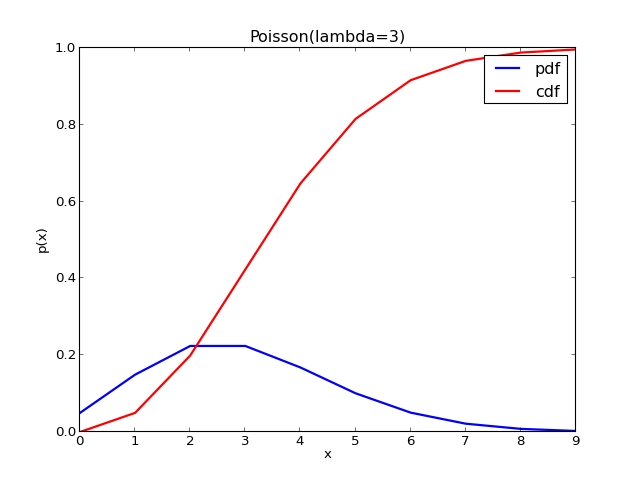
\includegraphics[width=4in]{images/poisson.png}
\caption{Example of Poisson distribution.}
\end{figure}

Intuitively, the meaning of $\lambda $ is the following:

Let"s consider a unitary time interval $T$ and divide it into
$n$ subintervals of the same size.
Let $p_n$ be the probability of one success occurring in a single
subinterval. For $T$ fixed when $n\rightarrow \infty , $ $p_n\rightarrow 0$
but the limit
\begin{equation}
\lim_{n\rightarrow \infty }pn
\end{equation}
is finite. This limit is $\lambda $.

We can use the same technique adopted for the
binomial distribution and observe that for Poisson, 
\begin{eqnarray}
\textrm{Prob}(X &=&0)=e^{-\lambda } \\
\textrm{Prob}(X &=&k+1)=\frac{^\lambda }{k+1}\textrm{Prob}(X=k)
\end{eqnarray}
therefore the preceding algorithm can be modified into

%%% META:FILE:nlib/randomgen.nim
\begin{lstlisting}[caption={in file: {\ft nlib/randomgen.nim}}]
proc poisson*(r: RandomSource, lamb: float, epsilon = 1e-6): int =
  var u = r.random()
  var q = exp(-lamb)
  var k = 0
  while true:
    if u < q + epsilon: return k
    u = u - q
    q = q * lamb / float(k + 1)
    k += 1
\end{lstlisting}

Note how this algorithm may take an arbitrary amount of time to generate a
Poisson distributed random number, but eventually it stops. If $u$ is very
close to $1$, it is possible that errors due to finite machine precision
cause the algorithm to enter into an infinite loop. The $+\varepsilon $ term
can be used to correct this unwanted behavior by choosing $\varepsilon$ relatively small compared with the precision required in the computation, but
larger than machine precision.

\goodbreak\section{Probability distributions for continuous random variables}

\goodbreak\subsection{Uniform in range}

A typical problem is generating random integers in a given range $[a, b]$, 
including the extreme. We can map uniform random numbers $y_i\in (0, 1)$
into integers by using the formula
\begin{equation}
h_i=a+\left\lfloor (b-a+1)y_i\right\rfloor
\end{equation}

%%% META:FILE:nlib/randomgen.nim
\begin{lstlisting}[caption={in file: {\ft nlib/randomgen.nim}}]
proc uniform*(r: RandomSource, a, b: float): float =
  a + (b - a) * r.random()
\end{lstlisting}

\goodbreak\subsection{Exponential distribution}
\index{distribution!exponential}

The exponential distribution is used to model Poisson processes, which are
situations in which an object initially in state A can change to state B
with constant probability per unit time $\lambda $. The time at which the
state actually changes is described by an exponential random variable with
parameter $\lambda $. Therefore the integral from $0$ to $T$ over $p(t)$ is
the probability that the object is in state $B$ at time $T$.

The probability mass function is given by

\begin{equation}
p(x)=\lambda e^{-\lambda x}
\end{equation}

The exponential distribution may be viewed as a continuous counterpart of
the geometric distribution, which describes the number of Bernoulli trials
necessary for a discrete process to change state. In contrast, the
exponential distribution describes the time for a continuous process to
change state.

Examples of variables that are approximately exponentially distributed are as follows:

\begin{itemize}
\item  the time until you have your next car accident

\item  the time until you get your next phone call

\item  the distance between mutations on a DNA strand

\item  the distance between roadkill
\end{itemize}

An important property of the exponential distribution is that it is
memoryless: the chance that an event will occur $s$ seconds from now does not depend on the past. In particular, it does not depend on how much time we have been waiting already. In a formula we can write this condition as

\begin{equation}
\textrm{Prob}(X>s+t|X>t)=\textrm{Prob}(X>s)
\end{equation}

Any process satisfying the preceding condition is a Poisson process. The number of events per time unit is given by the Poisson distribution, and the time interval between consecutive events is described by the exponential distribution.

\begin{figure}[ht]
\centering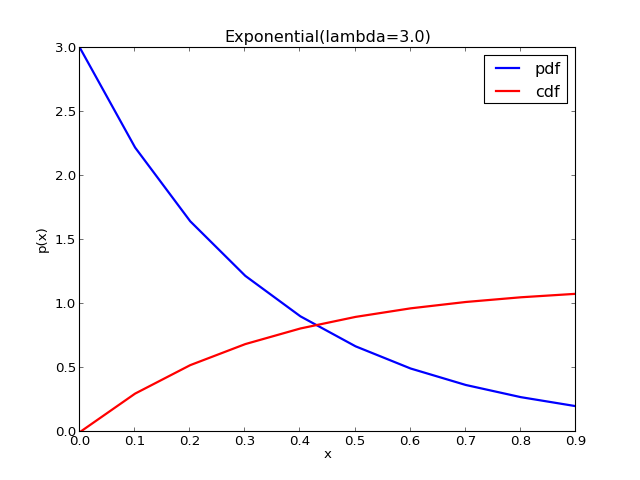
\includegraphics[width=4in]{images/exponential.png}
\caption{Example of exponential distribution.}
\end{figure}

The exponential distribution can be generated using the inversion method.
The scope is to determine a function $x=f(u)$ that maps a uniformly distributed variable $u$
into a continuous random variable $x$ with probability mass function $%
p(x)=\lambda e^{-\lambda x}$.

According to the inversion method, we proceed by computing $F$:
\begin{equation}
F(x) = \int_0^x p(y)dy=1-e^{-\lambda x}
\end{equation}
and we then invert $u=F(x)$, thus obtaining
\begin{equation}
x=-\frac 1\lambda \log (1-u)
\end{equation}
Now notice that if $u$ is uniform, $1-u$ is also uniform; therefore we can further simplify:
\begin{equation}
x=-\frac 1\lambda \log u
\end{equation}

We implement as follows:

%%% META:FILE:nlib/randomgen.nim
\begin{lstlisting}[caption={in file: {\ft nlib/randomgen.nim}}]
proc exponential*(r: RandomSource, lamb: float): float =
  -ln(r.random()) / lamb
\end{lstlisting}

This is an important distribution. Nim's {\ft std/random} does not ship with a built-in exponential generator, but the inversion-based one above ({\ft -ln(rand(1.0)) / lamb}) is a one-liner.

\goodbreak\subsection{Normal/Gaussian distribution}
\index{distribution!normal}
\index{distribution!Gaussian}

The normal distribution (also known as {\it Gaussian distribution})
is an extremely important probability distribution
considered in statistics. Here is the probability mass function:
\begin{equation}
p(x)=\frac 1{\sigma \sqrt{2\pi }}e^{-\frac{(x-\mu )^2}{2\sigma ^2}}
\end{equation}
where $E[X]=\mu $ and $E[(x-\mu )^2]=\sigma ^2$.

The standard normal distribution is the normal distribution with a mean of
0 and a standard deviation of 1. Because the graph of its probability
density resembles a bell, it is often called the {\it bell curve}.

The Gaussian distribution has two important properties:
\begin{itemize}
\item The average of many independent random variables with finite mean and finite variance tends to be a Gaussian distribution.
\item The sum of two independent Gaussian random variables with means $\mu_1$ and $\mu_2$ and variances $\sigma_1^2$ and $\sigma_2^2$ is also a Gaussian random variable with mean $\mu = \mu_1+\mu_2$ and variance $\sigma^2 = \sigma_1^2+\sigma_2^2$.
\end{itemize}

\begin{figure}[ht]
\centering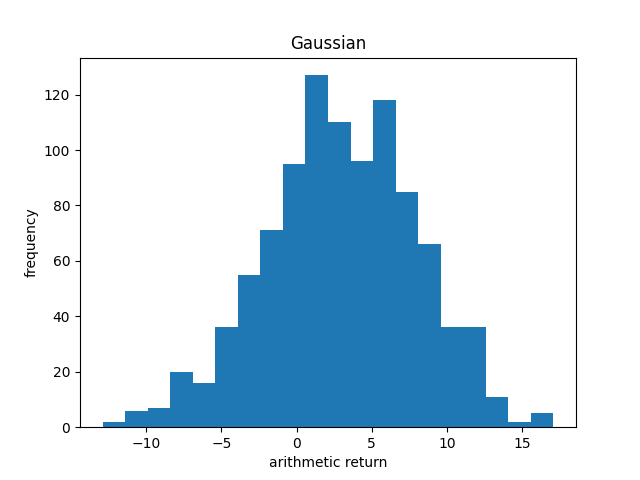
\includegraphics[width=4in]{images/gaussian.png}
\caption{Example of Gaussian distribution.}
\end{figure}

There is no way to map a uniform random number into a Gaussian number but there is an algorithm to generate two independent Gaussian random numbers ($y_1$ and $y_2$) using two independent uniform random numbers ($x_1$ and $x_2$):

\begin{itemize}
\item  computing $v_1=2x_1-1, v_2=2x_2-1$ and $s=v_1^2+v_2^2$
\item  if $s>1$ start again
\item  $y_1=v_1\sqrt{(-2/s)\log s}$ and $y_2=v_2\sqrt{(-2/s)\log s}$
\end{itemize}

%%% META:FILE:nlib/randomgen.nim
\begin{lstlisting}[caption={in file: {\ft nlib/randomgen.nim}}]
type
  GaussRandomSource* = ref object
    base*: RandomSource
    other*: Option[float]   # cached second value from Marsaglia pair

proc newGaussRandomSource*(base: RandomSource): GaussRandomSource =
  GaussRandomSource(base: base, other: none(float))

proc gauss*(g: GaussRandomSource, mu = 0.0, sigma = 1.0): float =
  ## Marsaglia polar method: produces two Gaussians per call;
  ## one is cached for the next invocation.
  var thisVal: float
  if g.other.isSome:
    thisVal = g.other.get()
    g.other = none(float)
  else:
    var v1, v2, r: float
    while true:
      v1 = g.base.uniform(-1.0, 1.0)
      v2 = g.base.uniform(-1.0, 1.0)
      r = v1 * v1 + v2 * v2
      if r < 1: break
    thisVal = sqrt(-2.0 * ln(r) / r) * v1
    g.other = some(sqrt(-2.0 * ln(r) / r) * v2)
  mu + sigma * thisVal
\end{lstlisting}

Note how the first time the method next is called, it generates two Gaussian
numbers ($this$ and $other$), stores $other$, and returns $this$. Every other
time, the method next is called if $other$ is stored, and it returns a number;
otherwise it recomputes $this$ and $other$ again.

To map a random Gaussian number $y$ with mean $0$ and standard deviation $1$
into another Gaussian number $y^{\prime }$ with mean $\mu $ and standard
deviation $\sigma $, 
\begin{equation}
y^{\prime }=\mu +y\sigma
\end{equation}
We used this relation in the last line of the code.

This is also an important distribution; Nim's {\ft std/random} provides it directly:

\begin{lstlisting}
import std/random
echo gauss(mu, sigma)
\end{lstlisting}

Given a Gaussian random variable with mean $\mu$ and standard deviation $\sigma$, it is often useful to know how many standard deviations $a$ correspond to a confidence $c$ defined as

\begin{equation}
c = \int_{\mu-a\sigma}^{\mu+a\sigma} p(x)\textrm{d}x
\end{equation}

The following algorithm generates a table of $a$ versus $c$ given $\mu$ and $\sigma$:

\index{confidence intervals}

%%% META:FILE:nlib/randomgen.nim
\begin{lstlisting}[caption={in file: {\ft nlib/randomgen.nim}}]
const CONFIDENCE* = [
  (0.68,    1.0),
  (0.80,    1.281551565545),
  (0.90,    1.644853626951),
  (0.95,    1.959963984540),
  (0.98,    2.326347874041),
  (0.99,    2.575829303549),
  (0.995,   2.807033768344),
  (0.998,   3.090232306168),
  (0.999,   3.290526731492),
  (0.9999,  3.890591886413),
  (0.99999, 4.417173413469)
]

proc confidenceIntervals*(mu, sigma: float): seq[(float, float, float)] =
  ## Returns (confidence, lower bound, upper bound) for a Gaussian.
  for (a, b) in CONFIDENCE:
    result.add (a, mu - b * sigma, mu + b * sigma)
\end{lstlisting}


\goodbreak\subsection{Pareto distribution}
\index{distribution!pareto}

The Pareto distribution, named after the economist Vilfredo Pareto, is a power law probability distribution that coincides with social, scientific, geophysical, actuarial, and many other types of observable phenomena. Outside the field of economics, it is sometimes referred to as the Bradford distribution. Its cumulative distribution function is

\begin{equation}
F(x) \equiv  \textrm{Prob}(X<x) = 1 - \left(\frac{x_m}{x}\right)^{\alpha}
\end{equation}

\begin{figure}[ht]
\centering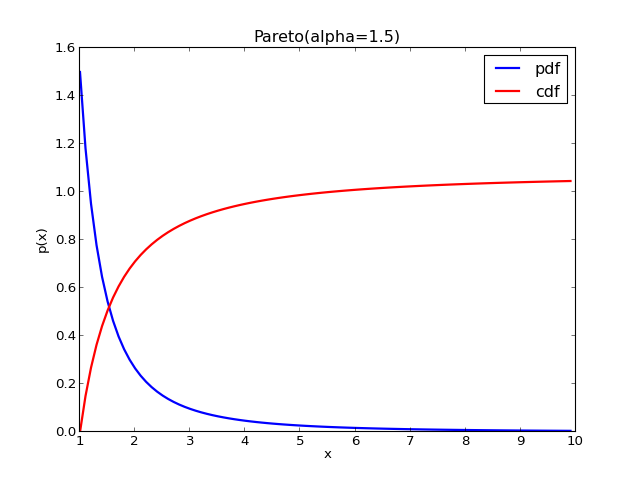
\includegraphics[width=4in]{images/pareto.png}
\caption{Example of Pareto distribution.}
\end{figure}

It can be implemented as follows using the inversion method:

%%% META:FILE:nlib/randomgen.nim
\begin{lstlisting}[caption={in file: {\ft nlib/randomgen.nim}}]
proc pareto*(r: RandomSource, alpha, xm: float): float =
  let u = r.random()
  xm * pow(1.0 - u, -1.0 / alpha)
\end{lstlisting}

When {\ft RandomSource} is not available, the same closed-form expression {\ft xm * pow(1.0 - rand(1.0), -1.0 / alpha)} can be used directly.

The Pareto distribution is an example of Levy distribution. The Central Limit theorem does not apply to it.

\goodbreak\subsection{In and on a circle}
\index{distribution!circle}

We can generate a random point $(x, y)$ uniformly distributed on a circle by generating a random angle.
\begin{eqnarray}
x &=&\cos (2\pi u) \\
y &=&\sin (2\pi u)
\end{eqnarray}

%%% META:FILE:nlib/randomgen.nim
\begin{lstlisting}[caption={in file: {\ft nlib/randomgen.nim}}]
proc pointOnCircle*(r: RandomSource, radius = 1.0): (float, float) =
  let angle = 2.0 * PI * r.random()
  (radius * cos(angle), radius * sin(angle))
\end{lstlisting}

We can generate a random point uniformly distributed inside a circle by generating, independently, the $x$ and $y$ coordinates of points inside a square and rejecting those outside the circle:

%%% META:FILE:nlib/randomgen.nim
\begin{lstlisting}[caption={in file: {\ft nlib/randomgen.nim}}]
proc pointInCircle*(r: RandomSource, radius = 1.0): (float, float) =
  while true:
    let x = r.uniform(-radius, radius)
    let y = r.uniform(-radius, radius)
    if x * x + y * y < radius * radius:
      return (x, y)
\end{lstlisting}

\goodbreak\subsection{In and on a sphere}
\index{distribution!sphere}

A random point $(x, y, z)$ uniformly distributed on a sphere of radius 1 is
obtained by generating three uniform random numbers $u_1, u_2, u_3, $; compute $%
v_i=2u_i-1$, and if $v_1^2+v_2^2+v_3^2\leq 1$, 
\begin{eqnarray}
x &=&v_1/\sqrt{v_1^2+v_2^2+v_3^2} \\
y &=&v_2/\sqrt{v_1^2+v_2^2+v_3^2} \\
z &=&v_3/\sqrt{v_1^2+v_2^2+v_3^2}
\end{eqnarray}
else start again.

%%% META:FILE:nlib/randomgen.nim
\begin{lstlisting}[caption={in file: {\ft nlib/randomgen.nim}}]
proc pointInSphere*(r: RandomSource, radius = 1.0):
                   (float, float, float) =
  while true:
    let x = r.uniform(-radius, radius)
    let y = r.uniform(-radius, radius)
    let z = r.uniform(-radius, radius)
    if x * x + y * y + z * z < radius * radius:
      return (x, y, z)

proc pointOnSphere*(r: RandomSource, radius = 1.0):
                   (float, float, float) =
  let (x, y, z) = r.pointInSphere(radius)
  let nrm = sqrt(x * x + y * y + z * z)
  (x / nrm, y / nrm, z / nrm)
\end{lstlisting}

\section{Resampling}
\index{resampling}

So far we always generated random numbers by modeling the random variable (e.g., uniform, or exponential, or Pareto) and using an algorithm to generate possible values of the random variables.

We now introduce a different methodology, which we will need later when talking about the bootstrap method.
If we have a population $S$ of equally distributed events and we need to generate an event from the same distribution as the population, we can simply draw a random element from the population. In Nim, {\ft std/random} provides the {\ft sample} procedure:

\begin{lstlisting}
import std/random
randomize()
let S = @[1, 2, 3, 4, 5, 6]
echo sample(S)
\end{lstlisting}

We can therefore generate a sample of random events by repeating this procedure. This is called {\it resampling}~\cite{resampling}:

%%% META:FILE:nlib/randomgen.nim
\begin{lstlisting}[caption={in file: {\ft nlib/randomgen.nim}}]
proc resample*[T](S: openArray[T], size = -1): seq[T] =
  let n = if size < 0: S.len else: size
  for _ in 0 ..< n: result.add sample(S)
\end{lstlisting}

\goodbreak\section{Binning}
\index{binning}

Binning is the process of dividing a space of possible events into
partitions and counting how many events fall into each partition. We can bin
the numbers generated by a pseudo random number generator and measure the
distribution of the random numbers.

Let"s consider the following program:
\begin{lstlisting}
import std/times

proc bin(generator: RandomSource, nevents: int,
         a, b: float, nbins: int): seq[float] =
  result = newSeq[float](nbins)
  for _ in 0 ..< nevents:
    let x = generator.random()
    if x >= a and x <= b:
      let k = int((x - a) / (b - a) * float(nbins))
      result[k] += 1.0
  for i in 0 ..< nbins:
    result[i] /= float(nevents)

proc testBin(nevents = 1000, nbins = 10) =
  let g = newRandomSource(
    proc(): float = newMCG(int(epochTime())).random())
  let bins = bin(g, nevents, 0.0, 1.0, nbins)
  for i, b in bins:
    echo i, " ", b

testBin()
\end{lstlisting}

It produces the following output:
\begin{lstlisting}
i frequency[i]
0 0.101
1 0.117
2 0.092
3 0.091
4 0.091
5 0.122
6 0.096
7 0.102
8 0.090
9 0.098
\end{lstlisting}

Note that

\begin{itemize}
\item  all bins have the same size 1/nbins;

\item  the size of the bins is normalized, and the sum of the values is 1

\item  the distribution of the events into bins approaches the distribution
of the numbers generated by the random number generator
\end{itemize}

As an experiment, we can do the same binning on a larger number of events, 
\begin{lstlisting}
>>> test_bin(100000)
\end{lstlisting}

which produces the following output:
\begin{lstlisting}
i frequency[i]
0 0.09926
1 0.09772
2 0.10061
3 0.09894
4 0.10097
5 0.09997
6 0.10056
7 0.09976
8 0.10201
9 0.10020
\end{lstlisting}

Note that these frequencies differ from 0.1 for less than 3\%, whereas some of
the preceding numbers differ from 0.11 for more than 20\%.

\chapter{Monte Carlo Simulations}
\index{Monte Carlo}

\goodbreak\section{Introduction}

Monte Carlo methods are a class of algorithms that rely on repeated random sampling to compute their results, which are otherwise deterministic.

\goodbreak\subsection{Computing $\pi$}

The standard way to compute $\pi $ is by applying the definition: $\pi $ is
the length of a semicircle with a radius equal to 1. From the definition, one can
derive an exact formula:
\begin{equation}
\pi =4\arctan 1
\end{equation}
The arctan has the following Taylor series expansion:\footnote{%
Taylor expansion:
\begin{equation}
f(x)=f(0)+f^{\prime }(0)x+\frac 1{2!}f^{\prime \prime }(0)x^2+...+\frac
1{i!}f^{(i)}(0)x^2+....
\end{equation}
\par
and if $f(x)=\arctan x$ then:
\begin{eqnarray}
f^{\prime }(x) &=&\frac{d\arctan x}{dx}=\frac 1{1+x^2}\rightarrow f^{\prime
}(0)=1 \\
f^{\prime \prime }(x) &=&\frac{d^2\arctan x}{d^2x}=\frac d{dx}\frac
1{1+x^2}=-\frac{2x}{(1+x^2)^2} \\
&&... \\
f^{(2i+1)}(x) &=&(-1)^i\frac{(2i)!}{(1+x^2)^{2i+1}}+x...\rightarrow
f^{(2i+1)}(0)=(-1)(2i)! \\
f^{(2i)}(x) &=&x...\rightarrow f^{(2i)}(0)=0
\end{eqnarray}
}:

\begin{equation}
\arctan x=\allowbreak \sum_{i=0}(-1)^i\frac{x^{2i+1}}{2i+1}
\end{equation}
and one can approximate $\pi $ to arbitrary precision by computing the sum
\begin{equation}
\pi =\allowbreak \sum_{i=0}(-1)^i\frac 4{2i+1}
\end{equation}

We can use the program
\begin{lstlisting}
proc piTaylor(n: int) =
  var pi = 0.0
  for i in 0 ..< n:
    pi = pi + 4.0 / float(2 * i + 1) * pow(-1.0, float(i))
    echo i, " ", pi

piTaylor(1000)
\end{lstlisting}

which produces the following output:
\begin{lstlisting}
0 4.0
1 2.66666...
2 3.46666...
3 2.89523...
4 3.33968...
...
999 3.14..
\end{lstlisting}

A better formula is due to Plauffe, 

\begin{equation}
\pi = \sum_{i=0} \frac{1}{16^i} \left(
\frac{4}{8i+1}-\frac{2}{8i+4}-\frac{1}{8i+5}-\frac{1}{8i+6}
\right)
\end{equation}

which we can implement as follows:
we can use the program
\begin{lstlisting}
# Nim does not ship with arbitrary-precision decimals in the stdlib;
# we use plain `float` here. For the high-precision form a `BigFloat`
# package such as `bignum` would replace the `float` type below.

proc piPlauffe(n: int): float =
  var pi = 0.0
  let a = 4.0
  let b = 2.0
  let c = 1.0
  let d = 1.0 / 16.0
  for i in 0 ..< n:
    let i8 = float(8 * i)
    pi += pow(d, float(i)) * (a/(i8+1.0) - b/(i8+4.0) -
                              c/(i8+5.0) - c/(i8+6.0))
  return pi

echo piPlauffe(1000)
\end{lstlisting}

The preceding formula works and converges very fast and already in 100 iterations produces
\begin{equation}
\pi = 3.1415926535897932384626433...
\end{equation}

There is a different approach based on the fact that $\pi$ is also the
area of a circle of radius 1. We can draw a square or area containing
a quarter of a circle of radius 1. We can randomly generate points $(x, y)$
with uniform distribution inside the square and check if the points fall inside
the circle. The ratio between the number of points that fall in
the circle over the total number of points is proportional to the area of
the quarter of a circle ($\pi /4$) divided by the area of the square (1).

Here is a program that implements this strategy:
\begin{lstlisting}
import std/random
randomize()

proc piMc(n: int) =
  var counter = 0
  for i in 0 ..< n:
    let x = rand(1.0)
    let y = rand(1.0)
    if x * x + y * y < 1.0:
      inc counter
    let pi = 4.0 * float(counter) / float(i + 1)
    echo i, " ", pi

piMc(1000)
\end{lstlisting}

The output of the algorithm is shown in fig.~\ref{pi-plot}.

\begin{figure}[ht]
\centering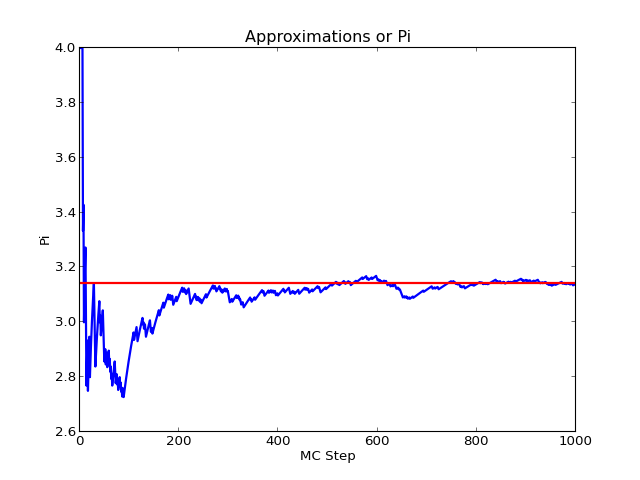
\includegraphics[width=4in]{images/pi.png}
\caption{Convergence of {\bf pi\_mc}.\label{pi-plot}}
\end{figure}

The convergence rate in this case is very slow, and this algorithm is of no practical value, but the methodology is sound, and for some problems, this method is the only one feasible.

Let"s summarize what we have done: we have formulated our problem (compute $%
\pi $) as the problem of computing an area (the area of a quarter of a
circle), and we have computed the area using random numbers. This is a
particular example of a more general technique known as a Monte Carlo
integration. In fact, the computation of an area is equivalent to the problem
of computing an integral.

Sometimes the formula is not known, or it is too complex to compute reliably, hence a Monte Carlo solution becomes preferable.


\goodbreak\subsection{Simulating an online merchant}

Let"s consider an online merchant. A website is visited many times a day.
From the logfile of the web application, we determine
that the average number of visitors in a day is 976, the number of
visitors is Gaussian distributed, and the standard deviation is 352. We also observe that each visitor has a 5\% probability of purchasing an item
if the item is in stock and a 2\% probability to buy an item if the
item is not in stock.

The merchant sells only one type of item that costs \$100 per unit. The
merchant maintains $N$ items in stock. The merchant pays \$30 a day to store
each unit item in stock. What is the optimal $N$ to maximize the average
daily income of the merchant?

This problem cannot easily be formulated analytically or reduced to
the computation of an integral, but it can easily be simulated.

In particular, we simulate many days and, for each day $i$, 
we start with $N$ items
in stock, and we loop over each simulated visitor. If the visitor
finds an item in stock, he buys it with a 5\% probability
(producing an income of \$70), whereas if the item is not in stock, 
 he buys it with 2\% probability (producing an income of \$100).
At the end of each day, we pay \$30 for each item remaining in stock.

Here is a program that takes $N$ (the number of items in stock) and $d$ (the
number of simulated days) and computes the average daily income:
\begin{lstlisting}
proc simulateOnce(N: int): float =
  var profit = 0.0
  let loss = 30.0 * float(N)
  var instock = N
  let visitors = int(gauss(976.0, 352.0))
  for _ in 0 ..< visitors:
    if instock > 0:
      if rand(1.0) < 0.05:
        instock -= 1
        profit += 100.0
    else:
      if rand(1.0) < 0.02:
        profit += 100.0
  profit - loss

proc simulateMany(N: int, ap = 1.0, rp = 0.01, ns = 1000): float =
  var s = 0.0
  var muOld = 0.0
  for k in 1 ..< ns:
    s += simulateOnce(N)
    let mu = s / float(k)
    if k > 10 and mu - muOld < max(ap, rp * mu):
      return mu
    muOld = mu
  raise newException(ArithmeticDefect, "no convergence")
\end{lstlisting}

By looping over different $N$ (items in stock), we can compute the average daily income as a function of $N$:
\begin{lstlisting}
for N in countup(0, 99, 10):
  echo N, " ", simulateMany(N, ap = 100.0)
\end{lstlisting}

The program produces the following output:
\begin{lstlisting}
n income
0 1955
10 2220
20 2529
30 2736
40 2838
50 2975
60 2944
70 2711
80 2327
90 2178
\end{lstlisting}

From this we deduce that the optimal number of items to carry in stock is
about 50. We could increase the resolution and precision of the simulation
by increasing the number of simulated days and reducing the step of the
amount of items in stock.

Note that the statement {\ft gauss(976, 352)} generates a random floating
point number with a Gaussian distribution centered at 976 and standard
deviation equal to 352, whereas the statement
\begin{lstlisting}
if random()<0.05:
\end{lstlisting}

ensures that the subsequent block is executed with a probability of 5\%.

The basic ingredients of every Monte Carlo simulation are here: (1) a function that simulates the system once and uses random variables to model unknown quantities; (2) a function that repeats the simulation many times to compute an average.

Any Monte Carlo solver comprises the following parts:

\begin{itemize}
\item A generator of random numbers (such as we have discussed in the previous chapter)
\item A function that uses the random number generator and can simulate the system once (we will call $x$ the result of each simulate once)
\item A function that calls the preceding simulation repeatedly and averages the results until they converge $\mu = \frac1N \sum x_i$
\item A function to estimate the accuracy of the result and determine when to stop the simulation, $\delta\mu < \textrm{precision}$
\end{itemize}

\section{Error analysis and the bootstrap method}

The result of any MC computation is an average:
\begin{equation}
\mu = \frac1N \sum x_i
\end{equation}

The error on this average can be estimated using the formula

\begin{equation}
\delta\mu = \frac{\sigma}{\sqrt{N}} = \sqrt{\frac1{N} \left( {\frac1N \sum x^2_i - \mu^2} \right)}
\end{equation}

This formula assumes the distribution of the $x_i$ is Gaussian. Using this formula, we can compute a 68\% confidence level for the MC computation of $\pi$, shown in fig.~\ref{pi-plot2}.

\begin{figure}[ht]
\centering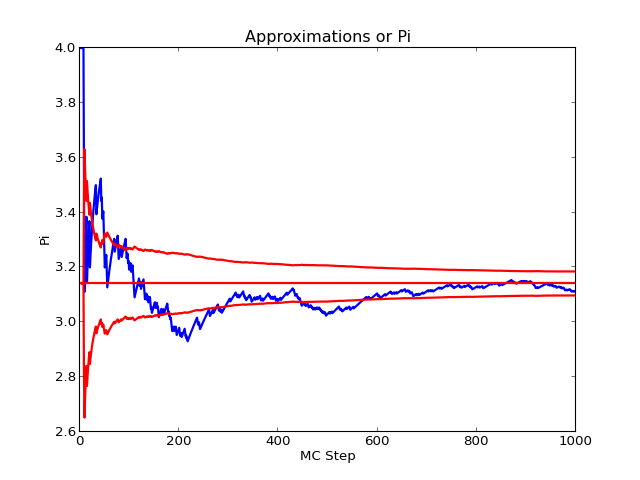
\includegraphics[width=4in]{images/pi2.png}
\caption{Convergence of $\pi$\label{pi-plot2}.}
\end{figure}

\index{bootstrap}

The purpose of the bootstrap~\cite{bootstrap} algorithm is computing the error in an average $\mu = (1/N) \sum x_i$ without making the assumption that the $x_i$ are Gaussian.

The first step of the bootstrap methodology consists of computing the average not only on the initial sample $\{x_i\}$ but also on many data samples obtained by resampling the original data. If the number of elements $N$ of the original sample were infinity, the average on each other sample would be the same. Because $N$ is finite, each of these means produces slightly different results:

\begin{equation}
\mu_k = \frac1N \sum x^{[k]}_i
\end{equation}

where $x^{[k]}_i$ is the $i$th element of resample $k$ and $\mu_k$ is the average of that resample.

The second step of the bootstrap methodology consists of sorting the $\mu_k$ and finding two values $\mu^-$ and $\mu^+$ that with a given percentage of the means follows in between those two values. The given percentage is the confidence level, and we set it to $68\%$.

Here is the complete algorithm:

%%% META:FILE:nlib/montecarlo.nim
\begin{lstlisting}[caption={in file: {\ft nlib/montecarlo.nim}}]
proc bootstrap*(x: seq[float], confidence = 0.68, nsamples = 100):
                (float, float, float) =
  ## Bootstrap confidence interval. Returns (lower, mean, upper).
  var means: seq[float] = @[]
  for _ in 0 ..< nsamples: means.add mean(resample(x))
  means.sort()
  let leftTail = int(((1.0 - confidence) / 2.0) * float(nsamples))
  let rightTail = nsamples - 1 - leftTail
  (means[leftTail], mean(x), means[rightTail])
\end{lstlisting}

Here is an example of usage:

\begin{lstlisting}
var S: seq[float] = @[]
for _ in 0 ..< 100: S.add gauss(2.0, 1.0)
echo bootstrap(S)
# (1.7767055865879007, 1.8968778392283303, 2.003420362236985)
\end{lstlisting}

In this example, the output consists of $\mu^-$, $\mu$, and $\mu^+$.

Because $S$ contains 100 random Gaussian numbers, with average 2 and standard deviation 1, we expect $\mu$ to be close to 2. We get $1.89$. The bootstrap tells us that with 68\% probability, the true average of these numbers is indeed between $1.77$ and $2.00$. The uncertainty $(2.00-1.77)/2 = 0.12$ is compatible with $\sigma/\sqrt{100} = 1/10 = 0.10$.

\goodbreak\section{A general purpose Monte Carlo engine}
\index{MCEngine}

We can now combine everything we have seen so far into a generic program that can be used to perform the most generic Monte Carlo computation/simulation:

\index{class!MCEngine}

%%% META:FILE:nlib/montecarlo.nim
\begin{lstlisting}[caption={in file: {\ft nlib/montecarlo.nim}}]
type
  MCEngine* = ref object of RootObj
    results*: seq[float]
    convergence*: bool

method simulateOnce*(e: MCEngine): float {.base.} =
  raise newException(CatchableError, "simulateOnce not implemented")

proc simulateMany*(e: MCEngine, ap = 0.1, rp = 0.1, ns = 1000):
                  (float, float, float) =
  e.results = @[]
  var s1 = 0.0
  var s2 = 0.0
  e.convergence = false
  for k in 1 ..< ns:
    let x = e.simulateOnce()
    e.results.add x
    s1 += x
    s2 += x * x
    let mu = s1 / float(k)
    let variance = s2 / float(k) - mu * mu
    let dmu = sqrt(variance / float(k))
    if k > 10 and abs(dmu) < max(ap, abs(mu) * rp):
      e.convergence = true
      break
  e.results.sort()
  bootstrap(e.results)
\end{lstlisting}

The preceding class has two methods:
\begin{itemize}
\item {\ft simulate\_once} is not implemented because the class is designed to be subclassed, and the method is supposed to be implemented for each specific computation.
\item {\ft simulate\_many} is the part that stays the same; it calls {\ft simulate\_once} repeatedly, computes average and error analysis, checks convergence, and computes bootstrap error for the result.
\end{itemize}

It is also useful to have a function, which we call {\bf var} (aka {\it value at risk}~\cite{wilmott}), which computes a numerical value so that the output of a given percentage of the simulations falls below that value:

%%% META:FILE:nlib/montecarlo.nim
\begin{lstlisting}[caption={in file: {\ft nlib/montecarlo.nim}}]
proc valueAtRisk*(e: MCEngine, confidence = 95): float =
  let index = int(0.01 * float(e.results.len) * float(confidence) + 0.999)
  if e.results.len - index < 5:
    raise newException(ArithmeticDefect, "not enough data, not reliable")
  e.results[index]
\end{lstlisting}

Now, as a first example, we can recompute $\pi$ using this class:

\index{class!PiSimulator}

\begin{lstlisting}
type PiSimulator = ref object of MCEngine
method simulateOnce(e: PiSimulator): float =
  let x = rand(1.0); let y = rand(1.0)
  if x * x + y * y < 1.0: 4.0 else: 0.0

let s = PiSimulator()
echo s.simulateMany()
# (2.1818181818181817, 2.909090909090909, 3.6363636363636362)
\end{lstlisting}

Our engine finds that the value of $\pi$ with 68\% confidence level is between $2.18$ and $3.63$, with the most likely value of $2.90$. Of course, this is incorrect, because it generates too few samples, but the bounds are correct, and that is what matters.

\subsection{Value at risk}\index{value at risk}

Let"s consider a business subject to random losses, for example, a large bank subject to theft from employees.
Here we will make the following reasonable assumptions (which have been verified with data):
\begin{itemize}
\item There is no correlation between individual events.
\item There is no correlation between the time when a loss event occurs and the amount of the loss.
\item The time interval between losses is given by the exponential distribution (this is a Poisson process).
\item The distribution of the loss amount is a Pareto distribution (there is a fat tail for large losses).
\item The average number of losses is 10 per day.
\item The minimum recorded loss is \$5000. The average loss is \$15, 000.
\end{itemize}

Our goal is to simulate one year of losses and to determine

\begin{itemize}
\item The average total yearly loss
\item How much to save to make sure that in 95\% of the simulated scenarios, the losses can be covered without going broke
\end{itemize}

From these assumptions, we determine that the $\lambda=10$ for the exponential distribution and $x_m=3000$ for the Pareto distribution. The mean of the Pareto distribution is $\alpha x_m/(\alpha-1) = 15, 000$, from which we determine that $\alpha = 1.5$.

We can answer the first questions (the average total loss) simply multiplying the average number of losses per year, $52\times5$, by the number of losses in one day, 10, and by the average individual loss, \$15, 000, thus obtaining

\begin{equation}
\textrm{[average yearly loss]} = \$39, 000, 000
\end{equation}

To answer the second question, we would need to study the width of the distribution. The problem is that, for $\alpha=1.5$, the standard deviation of the Pareto distribution is infinity, and analytical methods do not apply. We can do it using a Monte Carlo simulation:


%%% META:FILE:risk.nim
\begin{lstlisting}[caption={in file: {\ft risk.nim}}]
import nlib

type
  RiskEngine = ref object of MCEngine
    lamb*, xm*, alpha*: float

proc newRiskEngine(lamb, xm, alpha: float): RiskEngine =
  RiskEngine(lamb: lamb, xm: xm, alpha: alpha)

method simulateOnce(e: RiskEngine): float =
  var totalLoss = 0.0
  var t = 0.0
  while t < 260:
    let dt = -ln(rand(1.0)) / e.lamb
    let amount = e.xm * pow(1.0 - rand(1.0), -1.0 / e.alpha)
    t += dt
    totalLoss += amount
  totalLoss

proc main() =
  randomize()
  let s = newRiskEngine(lamb = 10.0, xm = 5000.0, alpha = 1.5)
  echo s.simulateMany(rp = 1e-4, ns = 1000)
  echo s.valueAtRisk(95)

main()
\end{lstlisting}

This produces the following output:

\begin{lstlisting}
(38740147.179054834, 38896608.25084647, 39057683.35621854)
45705881.8776
\end{lstlisting}

The output of {\ft simulate\_many} should be compatible with the true result (defined as the result after an infinite number of iterations and at infinite precision) within the estimated statistical error.

The output of the {\ft var} function answers our second questions: We have to save \$45, 705, 881 to make sure that in 95\% of cases our losses are covered by the savings.


\subsection{Network reliability}
\index{network reliability}

Let"s consider a network represented by a set of $n_{nodes}$ nodes and $%
n_{links}$ bidirectional links. Information
packets travel on the network. They can
originate at any node ({\ft start}) and be addressed to any other node ({\ft %
stop}). Each link of the network has a probability $p$ of transmitting the
packet (success) and a probability $(1-p)$ of dropping the packet (failure).
The probability $p$ is in general different for each link of the network.

We want to compute the probability that a packet
starting in {\ft start} finds a successful path to reach {\ft stop}. A path
is successful if, for a given simulation, all links in the path succeed in
carrying the packet.

The key trick in solving this problem is in finding the proper
representation for the network. Since we are not requiring to determine the
exact path but only proof of existence, we use the concept of equivalence classes.

We say that two nodes are in the same equivalence class if and only
if there is a successful path that connects the two nodes.

The optimal data structure to implement equivalence classes is {\ft DisjSets}, discussed in chapter 3.

To simulate the system, we create a class {\ft Network} that extends {\ft MCEngine}. It has a {\ft simulate\_once} method that tries to send a packet from {\ft start} to
{\ft stop} and simulates the network once. During the simulation each link of the network may be up or down with given probability. If there is a path connecting the {\ft start} node to the {\ft stop} node in which all links of the network are up, then the packet transfer succeeds. We use the DisjointSets to represent sets of nodes connected together. If there is a link up connecting a node from a set to a node in another set, then the two sets are joined. If, in the end, the {\ft start} and {\ft stop} nodes are found to belong to the same set, then there is a path and {\ft simulate\_once} returns 1, otherwise it returns 0.

\index{class!NetworkReliability}

%%% META:FILE:network.nim
\begin{lstlisting}[caption={in file: {\ft network.nim}}]
import nlib, std/random

type
  NetworkReliability = ref object of MCEngine
    nNodes*, start*, stop*: int
    links*: seq[(int, int, float)]

proc newNetworkReliability(nNodes, start, stop: int): NetworkReliability =
  NetworkReliability(nNodes: nNodes, start: start, stop: stop)

proc addLink(s: NetworkReliability, i, j: int,
             failureProbability: float) =
  s.links.add (i, j, failureProbability)

method simulateOnce(s: NetworkReliability): float =
  let nodes = newDisjointSets(s.nNodes)
  for (i, j, pf) in s.links:
    if rand(1.0) > pf:
      discard nodes.join(i, j)
  if nodes.joined(s.start, s.stop): 1.0 else: 0.0

proc main() =
  randomize()
  let s = newNetworkReliability(100, start = 0, stop = 1)
  for _ in 0 ..< 300:
    s.addLink(rand(99), rand(99), rand(1.0))
  echo s.simulateMany()

main()
\end{lstlisting}

\subsection{Critical mass}
\index{radioactive decays}\index{nuclear reactor}

Here we consider the simulation of a chain reaction in a fissile material, for example, the uranium in a nuclear reactor~\cite{neutron}. We assume a material is in a spherical shape of known radius. At each point there is a probability of a nuclear fission, which we model as the emission of two neutrons. Each of the two neutrons travels and hits an atom, thus causing another fission. The two neutrons are emitted in random opposite directions and travel a distance given by the exponential distribution. The new fissions may occur inside material itself or outside. If outside, they are ignored. If the number of fission events inside the material grows exponentially with time, we have a self-sustained chain reaction; otherwise, we do not.

Fig.~\ref{nuclear} provides a representation of the process.

\begin{figure}[ht]
\centering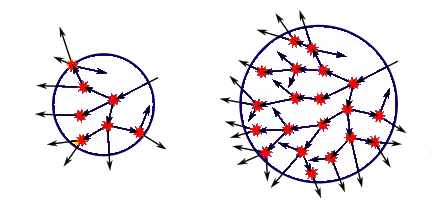
\includegraphics[width=4in]{images/critical.png}
\caption{Example of chain reaction within a fissile material. If the mass is small, most of the decay products escape (left, sub-criticality), whereas if the mass exceeds a certain critical mass, there is a self-sustained chain reaction (right).\label{nuclear}}
\end{figure}

\begin{figure}[ht]
\centering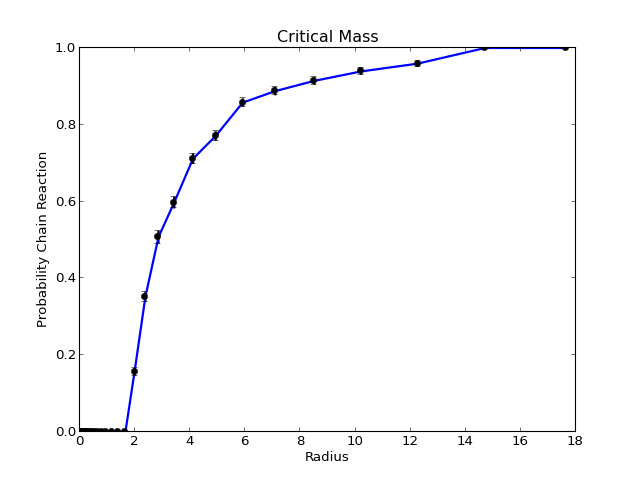
\includegraphics[width=4in]{images/nuclear.png}
\caption{Probability of chain reaction in uranium.\label{nuclear2}}
\end{figure}

Here is a possible implementation of the process. We store each event that happens inside the material in a queue ({\ft events}). For each simulation, the queue starts with one event, and from it we generate two more, and so on. If the new events happen inside the material, we place the new events back in the queue. If the size of the queue shrinks to zero, then we are subcritical. If the size of the queue grows exponentially, we have a self-sustained chain reaction. We detect this by measuring the size of the queue and whether it exceeds a threshold (which we arbitrarily set to 200). The average free flight distance for a neutron in  uranium is 1.91 cm. We use this number in our simulation. Given the radius of the material, {\ft simulate\_once} returns 1.0 if it detects a chain reaction and 0.0 if it does not. The output of {\ft simulate\_many} is the probability of a chain reaction:

\index{class!NuclearReactor}

%%% META:FILE:nuclear.nim
\begin{lstlisting}[caption={in file: {\ft nuclear.nim}}]
import nlib, std/random, std/math

type
  NuclearReactor = ref object of MCEngine
    radius*, density*: float
    threshold*: int

proc newNuclearReactor(radius: float, meanFreePath = 1.91,
                       threshold = 200): NuclearReactor =
  NuclearReactor(radius: radius, density: 1.0 / meanFreePath,
                 threshold: threshold)

proc pointOnSphereLocal(): (float, float, float) =
  while true:
    let x = rand(1.0); let y = rand(1.0); let z = rand(1.0)
    let d = sqrt(x*x + y*y + z*z)
    if d < 1: return (x/d, y/d, z/d)

method simulateOnce(s: NuclearReactor): float =
  var events: seq[(float, float, float)] = @[(0.0, 0.0, 0.0)]
  while events.len > 0:
    let p = events.pop()
    let (vx, vy, vz) = pointOnSphereLocal()
    let d1 = -ln(rand(1.0)) / s.density
    let d2 = -ln(rand(1.0)) / s.density
    let p1 = (p[0] + vx*d1, p[1] + vy*d1, p[2] + vz*d1)
    let p2 = (p[0] - vx*d2, p[1] - vy*d2, p[2] - vz*d2)
    if p1[0]^2 + p1[1]^2 + p1[2]^2 < s.radius:
      events.add p1
    if p2[0]^2 + p2[1]^2 + p2[2]^2 < s.radius:
      events.add p2
    if events.len > s.threshold:
      return 1.0
  return 0.0

proc main() =
  randomize()
  var data: seq[(float, float, float)] = @[]
  var radius = 0.01
  while radius < 21.0:
    let s = newNuclearReactor(radius)
    let r = s.simulateMany(ap = 0.01, rp = 0.01, ns = 1000)
    data.add (radius, r[1], (r[2] - r[0]) / 2.0)
    radius *= 1.2
  saveErrorbar("nuclear.png",
               data.mapIt(it[0]), data.mapIt(it[1]), data.mapIt(it[2]),
               title = "Critical Mass",
               xlab = "Radius",
               ylab = "Probability of chain reaction")

main()
\end{lstlisting}

Fig.~\ref{nuclear2} shows the output of the program, the probability of a chain reaction as function of the size of the uranium mass. We find a critical radius between 2 cm and 10 cm, which corresponds to a critical mass between 0.5 kg and 60 kg. The official number is 15 kg for uranium 233 and  60 kg for uranium 235. The lesson to learn here is that it is not safe to accumulate too much fissile material together. This simulation can be easily tweaked to determine the thickness of a container required to shield a radioactive material.

\section{Monte Carlo integration}
\index{integration!Monte Carlo}

\goodbreak\subsection{One-dimensional Monte Carlo integration}

Let"s consider a one-dimensional integral
\begin{equation}
I=\int_a^bf(x)dx
\end{equation}
Let"s now determine two functions $g(x)$ and $p(x)$ such that
\begin{equation}
p(x)=0\text{ for }x\in [-\infty , a]\cup [n, \infty ]
\end{equation}
and
\begin{equation}
\int_{-\infty }^{+\infty }p(x)dx=1
\end{equation}
and
\begin{equation}
g(x)=f(x)/p(x)
\end{equation}

We can interpret $p(x)$ as a probability mass function and
\begin{equation}
E[g(X)]=\int_{-\infty }^{+\infty }g(x)p(x)dx=\int_a^bf(x)dx=I
\end{equation}
Therefore we can compute the integral by computing the expectation value of
the function $g(X)$, where $X$ is a random variable with a distribution
(probability mass function) $p(x)$ different from zero in $[a, b]$ generated.

An obvious, although not in general an optimal choice, is
\begin{eqnarray}
&&p(x)\equiv \left\{
\begin{array}{ll}
1/(b-a) & \text{if }x\in [a, b] \\
0 & \text{otherwise}
\end{array}
\right\}   \label{defchoice} \\
&&g(x)\equiv (b-a)f(x)  \nonumber
\end{eqnarray}
so that $X$ is just a uniform random variable in $[a, b]$. Therefore
\begin{equation}
I=E\left[ g(X)\right] =\frac1N \sum_{i=0}^{i<N}g(x_i)
\end{equation}
This means that the integral can be evaluated by generating $N$ random
points $x_i$ with uniform distribution in the domain, evaluating the
integrand (the function $f$) on each point, averaging the results, and
multiplying the average by the size of the domain ($b-a$).

Naively, the error on the result can be estimated by computing the variance
\begin{equation}
\sigma ^2 = \frac 1N\sum_{i=0}^{i<N}\left[ g(x_i)-\left\langle
g\right\rangle \right] ^2
\end{equation}
with
\begin{equation}
\left\langle g\right\rangle = \frac 1N\sum_{i=0}^{i<N}g(x_i)
\end{equation}
and the error on the result is given by:
\begin{equation}
\delta I=\sqrt{\frac{\sigma ^2}{N}}
\end{equation}
The larger the set of sample points $N$, the lower the variance and the
error. The larger $N$, the better $E[g(X)]$ approximates the correct result $%
I$.

\index{class!MCIntegrator}

Here is a Nim program:

%%% META:FILE:integrate.nim
\begin{lstlisting}[caption={in file: {\ft integrate.nim}}]
import nlib, std/random, std/math

type
  MCIntegrator = ref object of MCEngine
    f*: proc(x: float): float
    a*, b*: float

proc newMCIntegrator(f: proc(x: float): float, a, b: float): MCIntegrator =
  MCIntegrator(f: f, a: a, b: b)

method simulateOnce(s: MCIntegrator): float =
  let x = s.a + (s.b - s.a) * rand(1.0)
  (s.b - s.a) * s.f(x)

proc main() =
  randomize()
  let s = newMCIntegrator(proc(x: float): float = sin(x), 0.0, 1.0)
  echo s.simulateMany()

main()
\end{lstlisting}

This technique is very general and can be extended to almost any integral
assuming the integrand is smooth enough on the integration domain.

The choice (\ref{defchoice}) is not always optimal because the integrand may
be very small in some regions of the integration domain and very large in
other regions. Clearly some regions contribute more than others to the
average, and one would like to generate points with a probability mass
function that is as close as possible to the original integrand. Therefore
we should choose a $p(x)$ according to the following conditions:

\begin{itemize}
\item  $p(x)$ is very similar and proportional to $f(x)$

\item  given $F(x)=\int_{-\infty }^xp(x)dx$, $F^{-1}(x)$ can be computed
analytically.
\end{itemize}

Any choice for $p(x)$ that makes the integration algorithm converge faster with less calls to {\ft simulate\_once} is called a {\it variance reduction technique}.

\goodbreak\subsection{Two-dimensional Monte Carlo integration}

The technique described earlier can easily be extended to two-dimensional integrals:
\begin{equation}
I=\int_{{\mathfrak D}}f(x_0, x_1)dx_0dx_1
\end{equation}
where ${\mathfrak D}$ is some two-dimensional domain. We determine two functions
$g(x_0, x_1)$ and $p_0(x_0), p_1(x_1)$ such that
\begin{equation}
p_0(x_0)=0\text{ or }p_1(x_1)=0\text{ for }x\notin {\mathfrak D}
\end{equation}
and
\begin{equation}
\int p_0(x_0)p_1(x_1)dx_0dx_1=1
\end{equation}
and
\begin{equation}
g(x_0, x_1)=\frac{f(x_0, x_1)}{p_0(x_0)p_1(x_1)}
\end{equation}

We can interpret $p(x_0, x_1)$ as a probability mass function for two
independent random variables $X_0$ and $X_1$ and
\begin{equation}
E[g(X_0, X_1)]=\int g(x_0, x_1)p_0(x_0)p_1(x_1)dx=\int_{{\mathfrak D}%
}f(x_0, x_1)dx_0dx_1=I
\end{equation}
Therefore
\begin{equation}
I = E[g(X_0, X_1)] = \frac 1N\sum_{i=0}^{i<N}g(x_{i0}, x_{i1})
\end{equation}

\goodbreak\subsection{$n$-dimensional Monte Carlo integration}

The technique described earlier can also be extended to $n$-dimensional integrals
\begin{equation}
I=\int_{{\mathfrak D}}f(x_0, ..., x_{n-1})dx_0...dx_{n-1}
\end{equation}
where ${\mathfrak D}$ is some $n$-dimensional domain identified by a function $%
domain(x_0, ..., x_{n-1})$ equal to 1 if ${\bf x}=(x_0, ..., x_{n-1})$ is in the
domain, 0 otherwise. We determine two functions $g(x_0, ..., x_{n-1})$ and $%
p(x_0, ..., x_{n-1})$ such that
\begin{equation}
p(x_0, ..., x_{n-1})=0\text{ for }x\notin {\mathfrak D}
\end{equation}
and
\begin{equation}
\int p(x_0, ..., x_{n-1})dx_0...dx_{n-1}=1
\end{equation}
and
\begin{equation}
g(x_0, ..., x_{n-1})=f(x_0, ..., x_{n-1})/p(x_0, ..., x_{n-1})
\end{equation}

We can interpret $p(x_0, ..., x_{n-1})$ as a probability mass function for $n$
independent random variables $X_0$...$X_{n-1}$ and
\begin{eqnarray}
E[g(X_0, ..., X_{n-1})] &=&\int g(x_0, ..., x_{n-1})p(x_0, ..., x_{n-1})dx \\
&=&\int_{{\mathfrak D}}f(x_0, ..., x_{n-1})dx_0...dx_{n-1}=I
\end{eqnarray}
Therefore
\begin{equation}
I=E[g(X_0, .., X_{n-1})] = \frac 1N\sum_{i=0}^{i<N}g({\bf x}_i)
\end{equation}
where for every point ${\bf x}_i$ is a tuple $(x_{i0}, x_{i1}, ..., x_{i, n-1})$.

As an example, we consider the integral
\begin{equation}
I = \int_0^1 dx_0 \int_0^1 dx_1 \int_0^1 dx_2 \int_0^1 dx_3 sin(x_0+x_1+x_2+x_3)
\end{equation}

Here is the code:
\begin{lstlisting}
type
  MCIntegrator4D = ref object of MCEngine
    f*: proc(x: array[4, float]): float

method simulateOnce(s: MCIntegrator4D): float =
  let volume = 1.0
  var x: array[4, float]
  while true:
    for d in 0 ..< 4: x[d] = rand(1.0)
    var s2 = 0.0
    for d in 0 ..< 4: s2 += x[d] * x[d]
    if s2 < 1.0: break
  volume * s.f(x)

let s = MCIntegrator4D(
  f: proc(x: array[4, float]): float = sin(x[0] + x[1] + x[2] + x[3]))
echo s.simulateMany()
\end{lstlisting}

\goodbreak\section{Stochastic, Markov, Wiener, and processes}

\index{stochastic process}
\index{Markov process}
\index{Wiener process}

A {\it stochastic process}~\cite{stochastic} is a random function, 
for example, a function that maps a
variable $n$ with domain $D$ into $X_n$, where $X_n$ is a random variable
with domain $R$. In practical applications, the domain $D$ over which the
function is defined can be a time interval (and the stochastic is called a
{\it time series}) or a region of space (and the stochastic process is
called a {\it random field}). Familiar examples of time series include {\it %
random walks}~\cite{rwalk}; stock market and exchange rate fluctuations; signals such as
speech, audio, and video; or medical data such as a patient"s EKG, EEG, blood
pressure, or temperature. Examples of random fields include static images, 
random topographies (landscapes), or composition variations of an
inhomogeneous material.

Let"s consider a grasshopper moving on a straight line, and let $X_n$ be the
position of the grasshopper at time $t=n\Delta _t$. Let"s also assume that at time 0, 
$X_0=0$. The position of the grasshopper at each future ($t>0$) time is unknown.
Therefore it is a random variable.

We can model the movements of the grasshopper as follows:

\begin{equation}
X_{n+1}=X_n + \mu + \varepsilon _n\Delta _x  \label{markov1}
\end{equation}
where $\Delta _x$ is a fixed step and $\varepsilon _n$ is a random variable
whose distribution depends on the model; $\mu$ is a constant drift term
(think of wind pushing the grasshopper in one direction).
It is clear that $X_{n+1}$ only
depends on $X_n$ and $\varepsilon _n$; therefore the probability distribution
of $X_{n+1}$ only depends on $X_n$ and the probability distribution of $%
\varepsilon _n$, but it does not depend on the past history of the grasshopper"s movements at
times $t<n\Delta _t$. We can write the statement by saying that
\begin{equation}
\textrm{Prob}(X_{n+1}=x|\{X_i\}\text{ for }i\leq n)=\textrm{Prob}(X_{n+1}=x|X_n)  \label{markov2}
\end{equation}

A process in which the probability distribution of its future state only
depends on the present state and not on the past is called a
{\it Markov process}~\cite{markov}.

To complete our model, we need to make additional assumptions about the
probability distribution of $\varepsilon _n$. We consider the two following cases:

\begin{itemize}
\item  $\varepsilon _n$ is a random variable with a Bernoulli distribution ($%
\varepsilon _n=+1$ with probability $p$ and $\varepsilon _n=-1$ with
probability $1-p$).

\item  $\varepsilon _n$ is a random variable with a normal (Gaussian)
distribution with probability mass function $p(\varepsilon
)=e^{-\varepsilon ^2/2}$. Notice that the previous case (Bernoulli) is equivalent to this case (Gaussian) over long time intervals because the sum of many independent Bernoulli variables approaches a Gaussian distribution.
\end{itemize}

A continuous time stochastic process (when
$\varepsilon _n$ is a continuous random number)
is called a {\it Wiener process}~\cite{wiener}.

The specific case when $\varepsilon _n$ is a Gaussian random variable is called an {\it Ito process}~\cite{ito}. An Ito process is also a Wiener process.

\goodbreak\subsection{Discrete random walk (Bernoulli process)}
\index{random walk}
\index{Bernoulli process}

Here we assume a discrete  random walk: $\varepsilon _n$ equal to
$+1$ with probability $p$ and equal to $-1$ with probability $1-p.$ We
consider discrete time intervals of equal length $\Delta _t$; at each time
step, if $\varepsilon _n=+1$, the grasshopper moves forward one unit ($\Delta _x$)
with probability $p$, and if $\varepsilon _n=-1$, he moves backward one
unit ($-\Delta _x$) with probability $1-p$.

For a total $n$ steps, the probability of moving $n_{+}$ steps in a positive
direction and $n_{-}=n-n_{+}$ in a negative direction is given by
\begin{equation}
\frac{n!}{n_{+}!(n-n_{+})!}p^{n_{+}}(1-p)^{n-n_{+}}
\end{equation}

The probability of going from $a=0$ to $b=k\Delta _x>0$ in a time $t=n\Delta
_t>0$ corresponds to the case when
\begin{eqnarray}
n &=&n_{+}+n_i \\
k &=&n_{+}-n_{-}
\end{eqnarray}
that solved in $n_{+}$ gives $n_{+}=(n+k)/2$, and therefore the probability
of going from $0$ to $k$ in time $t=n\Delta _t$ is given by
\begin{equation}
\textrm{Prob}(n, k)=\frac{n!}{((n+k)/2)!((n-k)/2)!}p^{(n+k)/2}(1-p)^{(n-k)/2}
\end{equation}

Note that $n+k$ has to be even, otherwise it is not possible for the
grasshopper to reach $k\Delta _x$ in exactly $n$ steps.

For large $n$, the following distribution in $k/n$ tends to a Gaussian distribution.

\goodbreak\subsection{Random walk: Ito process}
\index{Ito process}

Let"s assume an Ito process for our random walk: $\varepsilon _n$ is normally
(Gaussian) distributed. We consider discrete time intervals of equal length $%
\Delta _t$, at each time step if $\varepsilon _n=\varepsilon $ with
probability mass function $p(\varepsilon )=e^{-\varepsilon ^2/2}$. It turns
out that eq.(\ref{markov1}) gives
\begin{equation}
X_n = n \mu + \Delta _x\sum_{i=0}^{i<n}\varepsilon _i
\end{equation}
Therefore the location of the random walker at time $t=n\Delta _t$ is given
by the sum of $n$ normal (Gaussian) random variables:
\begin{equation}
p(X_n)=\frac 1{\sqrt{2\pi n\Delta _x^2}}e^{-(X_n - n\mu)^2/(2n\Delta _x^2)}
\end{equation}
Notice how the mean and the variance of $X_n$ are both proportional
to $n$, whereas the standard deviation is proportional to $\sqrt{n}$.

\begin{eqnarray}
\textrm{Prob}(a &\leq &X_n\leq b)=\frac 1{\sqrt{2\pi n\Delta _x^2}}\int_a^be^{-(X_n - n\mu)^2/(2n%
\Delta _x^2)}dx \\
&=&\frac 1{\sqrt{2\pi }}\int_{(a-n\mu)/(\sqrt{n}\Delta _x)}^{(b-n\mu)/(\sqrt{n}\Delta
_x)}e^{-x^2/2}dx \\
&=&\textrm{erf}(\frac {b-n\mu}{\sqrt{n}\Delta _x})-\textrm{erf}(\frac {a-n\mu}{\sqrt{n}\Delta
_x})
\end{eqnarray}

\goodbreak\section{Option pricing}
\index{Options}

A European call option is a contract that depends on an asset $S$. The contract gives the buyer of the contract the right (the option) to buy $S$ at a fixed price $A$ some time in the future, even if the actual price $S$ may be different. The actual current price of the asset is called the {\it spot price}. The buyer of the option hopes that the price of the asset, $S_t$, will exceed $A$, so that he will be able to buy it at a discount, sell it at market price, and make a profit. The seller of the option hopes this does not happen, so he earns the full sale price. For the buyer of the option, the worst case scenario is not to be able to recover the price paid for the option, but there is no best case because, hypothetically, he can make an arbitrarily large profit. For the seller, it is the opposite. He has an unlimited liability.

In practice, a call option allows a buyer to sell risk (the risk of the price of $S$ going up) to the seller. He pays a price for it, the cost of the option. This is a form of insurance. There are two types of people who trade options: those who are willing to pay to get rid of risk (because they need the underlying asset and want it at a guaranteed price) and those who simply speculate (buy risk and sell insurance). On average, speculators make money because, if they sell many options, risk averages out, and they collect the premiums (the cost of the options).

The European option has a term or expiration, $\tau$. It can only be exercised at expiration. The amount $A$ is called the {\it strike price}.

The value at expiration of a European call option is
\begin{equation}
\max (S_\tau -A, 0)
\end{equation}

Its present value is therefore

\begin{equation}
\max (S_\tau -A, 0) e^{-r\tau}
\end{equation}

where $r$ is the risk-free interest rate. This value corresponds to how much we would have to borrow today from a bank so that we can repay the bank at time $\tau$ with the profit from the option.

All our knowledge about the future spot price $x=S_\tau $ of the underlying
asset can be summarized into a probability mass function $p_\tau (x)$. Under
the assumption that $p_\tau (x)$ is known to both the buyer and the seller
of the option, it has to be that the averaged net present value of the
option is zero for any of the two parties to want to enter into the contract.
Therefore
\begin{equation}
C_{call}=e^{-r\tau }\int_{-\infty }^{+\infty }\max (x-A, 0)p_\tau (x)dx
\label{call_option}
\end{equation}


Similarly, we can perform the same computations for a put option. A put option gives the buyer the option to sell the asset on a given day at a fixed price. This is an insurance against the price going down instead of going up. The value of this option at expiration is

\begin{equation}
\max (A-S_\tau, 0)
\end{equation}

and its pricing formula is

\begin{equation}
C_{put}=e^{-r\tau }\int_{-\infty }^{+\infty }\max (A-x, 0)p_\tau (x)dx
\label{put_option}
\end{equation}

Also notice that $C_{call}-C_{put} = S_0 - A e^{-r\tau }$.
This relation is called the {\it call-put parity}.

Our goal is to model $p_\tau(x)$, the distribution of possible prices for the underlying asset at expiration of the option, and compute the preceding integrals using Monte Carlo.

\goodbreak\subsection{Pricing European options: Binomial tree}
\index{binomial tree}

To price an option, we need to know $p_\tau (S_\tau )$. This means we need to
know something about the future behavior of the price $S_\tau $ of the
underlying asset $S$ (a stock, an index, or something else). In absence of
other information (crystal ball or illegal insider"s information), one may
try to gather information from a statistical analysis of the past historic
data combined with a model of how the price $S_\tau $ evolves as a function of
time. The most typical model is the binomial model, which is a Wiener
process. We assume that the time evolution of the price of the asset $X$ is a
stochastic process similar to a random walk. We divide time into
intervals of size $\Delta _t$, and we assume that in each time interval $\tau
=n\Delta _t$, the variation in the asset price is
\begin{eqnarray}
S_{n+1} &=&S_nu\text{ with probability }p \\
S_{n+1} &=&S_nd\text{ with probability }1-p
\end{eqnarray}
where $u>1$ and $0<d<1$ are measures for historic data. It follows that for $%
\tau =n\Delta _t$, the probability that the spot price of the asset at
expiration is $S_uu^id^{n-i}$ is given by

\begin{equation}
\textrm{Prob}(S_\tau =S_uu^id^{n-i})=\binom nip^i(1-p)^{n-i}
\end{equation}
and therefore
\begin{equation}
C_{call}=e^{-r\tau }\frac 1n\sum_{i=0}^{i\leq n}\binom nip^i(1-p)^{n-i}\max
(S_uu^id^{n-i}-A, 0)  \label{bincall}
\end{equation}
and
\begin{equation}
C_{put}=e^{-r\tau }\frac 1n\sum_{i=0}^{i\leq n}\binom nip^i(1-p)^{n-i}\max
(A-S_uu^id^{n-i}, 0)  \label{binput}
\end{equation}

The parameters of this model are $u, d$ and $p$, and they must be determined
from historical data. For example, 

\begin{eqnarray}
p &=& \frac{e^{r\Delta_t} - d}{u-d} \\
u &=& e^{\sigma\sqrt{\Delta_t}} \\
d &=& e^{-\sigma\sqrt{\Delta_t}}
\end{eqnarray}

where $\Delta_t$ is the length of the time interval, $r$ is the risk-free rate, and $\sigma$ is the volatility of the asset, that is, the standard deviation of the log returns.

Here is the code to simulate an asset price using a binomial tree:
\begin{lstlisting}
proc binomialSimulation(S0, u, d, p: float, n: int): seq[float] =
  var S = S0
  for _ in 0 ..< n:
    result.add S
    if rand(1.0) < p: S = u * S
    else:             S = d * S
\end{lstlisting}

The function takes the present spot value, $S_0$, of the asset, the values
of $u, d$ and $p$, and the number of simulation steps and returns a list
containing the simulated evolution of the stock price. Note that because of
the exact formulas, eqs.(\ref{bincall}) and (\ref{binput}), one does not need
to perform a simulation unless the underlying asset is a stock that pays
dividends or we want to include some other variable in the model.

This method works fine for European call options, but the method is not easy to
generalize to other options, when it depends on the path of
the asset (e.g., the asset is a stock that pays dividends). Moreover, 
to increase precision, one has to decrease $\Delta _t$ or redo the
computation from the beginning.

The Monte Carlo method that we see next is slower in the simple cases but is
more general and therefore more powerful.

\goodbreak\subsection{Pricing European options: Monte Carlo}

Here we adopt the Black--Scholes model assumptions.
We assume that the time evolution of the price of the asset $X$ is
a stochastic process similar to a random walk~\cite{shreve}. We divide time into
intervals of size $\Delta _t$, and we assume that in each time interval $%
t=n\Delta _t$, the log return is a Gaussian random variable:
\begin{equation}
\log \frac{S_{n+1}}{S_n} = \textrm{gauss}(\mu\Delta_t, \sigma\sqrt{\Delta_t}) \label{BS}
\end{equation}

There are three parameters in the preceding equation:

\begin{itemize}
\item  $\Delta _t$ is the time step we use in our discretization. $\Delta _t$
is not a physical parameter; it has nothing to do with the asset. It has to
do with the precision of our computation. Let"s assume that $\Delta _t=1$ day.

\item  $\mu $ is a drift term, and it represents the expected rate of return
of the asset over a time scale of one year. It is usually set equal to the risk-free rate.

\item  $\sigma $ is called volatility, and it represents the number of
stochastic fluctuations of the asset over a time interval of one year.
\end{itemize}

Notice that this model is equivalent to the previous binomial model for large time intervals, in the same sense as the binomial distribution for large values of $n$ approximates the Gaussian distribution. For large $T$, converge to the same result.

Notice how our assumption that log-return is Gaussian is different and not compatible with Markowitz"s assumption of modern portfolio theory (the arithmetic return is Gaussian). In fact, log returns and arithmetic returns cannot both be Gaussian. It is therefore incorrect to optimize a portfolio using MPT when the portfolio includes options priced using Black--Scholes. The price of an individual asset cannot be negative, therefore its arithmetic return cannot be negative and it cannot be Gaussian. Conversely, a portfolio that includes both short and long positions (the holder is the buyer and seller of options) can have negative value. A change of sign in a portfolio is not compatible with the Gaussian log-return assumption.

If we are pricing a European call option, we are only interested in $S_T$ and not in $S_t$ for $0<t<T$; therefore we can choose $\Delta_t = T$. In this case, we obtain

\begin{equation}
S_T = S_0 exp(r_T)
\end{equation}

and

\begin{equation}
p(r_T) \propto \exp\left(-\frac{(r_T-\mu T)^2}{2\sigma^2 T}\right)
\end{equation}

This allows us to write the following:

%%% META:FILE:options.nim
\begin{lstlisting}[caption={in file: {\ft options.nim}}]
import nlib, std/random, std/math

type
  EuropeanCallOptionPricer = ref object of MCEngine
    spotPrice*, mu*, sigma*, strike*, riskFreeRate*: float
    timeToExpiration*: int

proc presentValue(p: EuropeanCallOptionPricer, payoff: float): float =
  let dailyReturn = p.riskFreeRate / 250.0
  payoff * exp(-dailyReturn * float(p.timeToExpiration))

method simulateOnce(p: EuropeanCallOptionPricer): float =
  let T = float(p.timeToExpiration)
  let S = p.spotPrice
  let rT = gauss(p.mu * T, p.sigma * sqrt(T))
  let ST = S * exp(rT)
  let payoff = max(ST - p.strike, 0.0)
  p.presentValue(payoff)

proc main() =
  randomize()
  let pricer = EuropeanCallOptionPricer(
    spotPrice: 100.0,
    mu: 0.12 / 250.0,
    sigma: 0.30 / sqrt(250.0),
    strike: 110.0,
    timeToExpiration: 90,
    riskFreeRate: 0.05)
  echo pricer.simulateMany(ap = 0.01, rp = 0.01)

main()
\end{lstlisting}

\goodbreak\subsection{Pricing any option with Monte Carlo}

An option is a contract, and one can write a contract with many different clauses. Each of them can be implemented into an algorithm. Yet we can group them into three different categories:
\begin{itemize}
\item Non-path-dependent: They depend on the price of the underlying asset at expiration but not on the intermediate prices of the asset (path).
\item Weakly path-dependent: They depend on the price of the underlying asset and events that may happen to the price before expiration, but they do not depend on when the events exactly happen.
\item Strongly path-dependent: They depend on the details of the time variation of price of the underlying asset before expiration.
\end{itemize}

 Because non-path-dependent options do not depend on details, it is often possible to find approximate analytical formulas for pricing the option. For weakly path-dependent options, usually the binomial tree approach of the previous section is a preferable approach. The Monte Carlo approach applies to the general case, for example, that of strongly path-dependent options.

We will use our {\ft MCEngine} to implement a generic option pricer.

First we need to recognize the following:\index{payoff}

\begin{itemize}
\item  The value of an option at expiration is defined by a payoff function
$f(x)$ of the spot price of the asset at the expiration date. The fact that
a call option has payoff $f(x)=\max (x-A, 0)$ is a convention that defined the European call option.
A different type of option will have a different payoff function $f(x)$.

\item  The more accurately we model the underlying asset, the more accurate will be the computed value of the option. Some options are more sensitive than others to our modeling details.
\end{itemize}

Note one never models the option. One only models the underlying asset. The option payoff is given. We only choose the most efficient algorithm based on the model and the option:

%%% META:FILE:options.nim
\begin{lstlisting}[caption={in file: {\ft options.nim}}]
import nlib, std/random, std/math

type
  GenericOptionPricer = ref object of MCEngine
    spotPrice*, mu*, sigma*, strike*, riskFreeRate*: float
    timeToExpiration*: int
    payoff*: proc(p: GenericOptionPricer, path: seq[float]): float

proc model(p: GenericOptionPricer, dt = 1.0): float =
  gauss(p.mu * dt, p.sigma * sqrt(dt))

proc presentValue(p: GenericOptionPricer, payoff: float): float =
  let dailyReturn = p.riskFreeRate / 250.0
  payoff * exp(-dailyReturn * float(p.timeToExpiration))

method simulateOnce(p: GenericOptionPricer): float =
  var S = p.spotPrice
  var path = @[S]
  for _ in 0 ..< p.timeToExpiration:
    let r = p.model()
    S = S * exp(r)
    path.add S
  p.presentValue(p.payoff(p, path))

proc payoffEuropeanCall(p: GenericOptionPricer, path: seq[float]): float =
  max(path[^1] - p.strike, 0.0)

proc payoffEuropeanPut(p: GenericOptionPricer, path: seq[float]): float =
  max(p.strike - path[^1], 0.0)

proc payoffExoticCall(p: GenericOptionPricer, path: seq[float]): float =
  let last5 = path[^5 .. ^1]
  var s = 0.0
  for v in last5: s += v
  max(s / float(last5.len) - p.strike, 0.0)

proc main() =
  randomize()
  let pricer = GenericOptionPricer(
    spotPrice: 100.0,
    mu: 0.12 / 250.0,
    sigma: 0.30 / sqrt(250.0),
    strike: 110.0,
    timeToExpiration: 90,
    riskFreeRate: 0.05,
    payoff: payoffEuropeanCall)
  echo pricer.simulateMany(ap = 0.01, rp = 0.01)

main()
\end{lstlisting}

This code allows us to price any option simply by changing the payoff function.

One can also change the model for the underlying using different assumptions. For example, a possible choice is that of including a model for market crashes, and on random days, separated by intervals given by the exponential distribution, assume a negative jump that follows the Pareto distribution (similar to the losses in our previous risk model). Of course, a change of the model requires a recalibration of the parameters.

\begin{figure}[ht]
\centering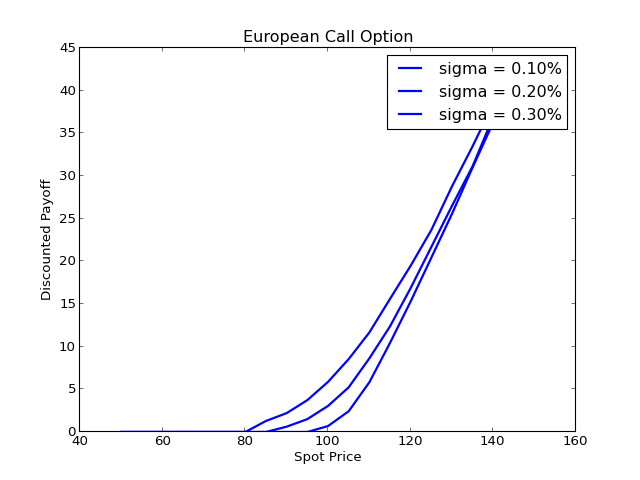
\includegraphics[width=4in]{images/option.png}
\caption{Price for a European call option for different spot prices and different values of $\sigma$.\label{options}}
\end{figure}

\section{Markov chain Monte Carlo (MCMC) and Metropolis}
\index{Markov chain}
\index{Metropolis algorithm}

Until this point, all our simulations were based on independent random
variables. This means that we were able to generate each random number
independently of the others because all the random variables were
uncorrelated. There are cases when we have the following problem.

We have to generate ${\bf x}=x_0, x_1, ..., x_{n-1}$, where $x_0, x_1, ..., x_{n-1}$
are $n$ correlated random variables whose probability mass function
\begin{equation}
p({\bf x})=p(x_0, x_1, ..., x_{n-1})
\end{equation}
cannot be factored, as in $p(x_0, x_1, ..., x_{n-1})=p(x_0)p(x_1)...p(x_{n-1})$. Consider for example the simple case of generating two random numbers $x_0$
and $x_1$ both in $[0, 1]$ with probability mass function $%
p(x_0, x_1)=6(x_0-x_1)^2$ (note that $\int_0^1\int_0^16p(x_0, x_1)dx_0dx_1=1$, 
as it should be).

In the case where each of the $x_i$ has a Gaussian distribution and the only dependence between $x_i$ and $x_j$ is their correlation, the solution was already examined in a previous section about the Cholesky algorithm. Here we examine the most general case.

The Metropolis algorithm provides a general and simpler solution to this problem. It is not always the most efficient, but more sophisticated algorithms are nothing but refinements and extensions of its simple idea.

Let"s formulate the problem once more: we want to generate ${\bf x}%
=x_0, x_1, ..., x_{n-1}$ where $x_0, x_1, ..., x_{n-1}$ are $n$ correlated random
variables whose probability mass function is given by
\begin{equation}
p({\bf x})=p(x_0, x_1, ..., x_{n-1})
\end{equation}

The procedure works as follows:

\begin{description}
\item[1]  Start with a set of independent random numbers ${\bf x}%
^{(0)}=(x_0^{(0)}, x_1^{(0)}, ..., x_{n-1}^{(0)})$ in the domain.

\item[2]  Generate another set of independent random numbers ${\bf x}%
^{(i+1)}=(x_0^{(i+1)}, x_1^{(i+1)}, ..., x_{n-1}^{(i+1)})$ in the domain. This can be done by an arbitrary random function $Q({\bf x}^{(i)})$. The only requirement for this function $Q$ is that the probability of moving from a current point $x$ to a new point $y$ be the same as that of moving from a current point $y$ to a new point $x$.

\item[3]  Generate a uniform random number $z$.

\item[4]  If $p({\bf x}^{(i+1)})/p({\bf x}^{(i)})<z$, then ${\bf x}^{(i+1)}=%
{\bf x}^{(i)}$.

\item[5]  Go back to step 2.
\end{description}

The set of random numbers ${\bf x}^{(i)}$ generated in this way for large
values of $i$ will have a probability mass function given by $p({\bf x})$.

Here is a possible implementation in Nim using an iterator:
\begin{lstlisting}
iterator metropolis(p: proc(x: seq[float]): float,
                    q: proc(x: seq[float]): seq[float],
                    x0: seq[float]): seq[float] =
  var x = x0
  while true:
    let xOld = x
    x = q(x)
    if p(x) / p(xOld) < rand(1.0):
      x = xOld
    yield x

proc P(x: seq[float]): float = 6.0 * (x[0] - x[1]) ^ 2
proc Q(x: seq[float]): seq[float] = @[rand(1.0), rand(1.0)]

var i = 0
for x in metropolis(P, Q, @[0.0, 0.0]):
  echo x
  inc i
  if i == 100: break
\end{lstlisting}

In this example, {\ft Q} is the function that generates random points in the domain (in the example, $[0, 1]\times[0, 1]$), and ${\ft P}$ is an example probability $p(x) = 6(x_0-x_1)^2$. We used a Nim {\ft iterator} with the {\ft yield} keyword instead of a {\ft proc} with {\ft return}: each {\ft yield} hands a value back to the {\ft for} loop, so values are generated lazily, one at a time, on demand.

\index{decorrelation}

Notice that the Metropolis algorithm can generate (and will generate) repeated values. This is because the next random vector $x$ is highly correlated with the previous vector. For this reason, it is often necessary to de-correlate metropolis values by skipping some of them:

\begin{lstlisting}
iterator metropolisDecorrelate(p: proc(x: seq[float]): float,
                               q: proc(x: seq[float]): seq[float],
                               x0: seq[float], ds = 100): seq[float] =
  var k = 0
  for x in metropolis(p, q, x0):
    inc k
    if k mod ds == ds - 1:
      yield x
\end{lstlisting}

The value of {\ft ds} must be fixed empirically. The value of {\ft ds} which is large enough to make the next vector independent from the previous one is called {\it decorrelation length}. This generator works as the previous one. For example:

\begin{lstlisting}
var i = 0
for x in metropolisDecorrelate(P, Q, @[0.0, 0.0]):
  echo x
  inc i
  if i == 100: break
\end{lstlisting}


\subsection{The Ising model}
\index{Ising model}

A typical example of application of the Metropolis is the Ising model. This model describes a spin system, for example, a ferromagnet. A spin system consists of a regular crystalline structure, and each vertex is an atom. Each atom is a small magnet, and its magnetic orientation can be +1 or $-$1. Each atom interacts with the external magnetic field and with the magnetic field of its six neighbors (think about the six faces of a cube). We use the index $i$ to label an atom and $s_i$ its spin.

The entire system has a total energy given by

\begin{equation}
E(s) = - \sum_i s_i h - \sum_{ij|dist_{ij}=1} s_i s_j
\end{equation}

where $h$ is the external magnetic field, the first sum is over all spin sites, and the second is about all couples of next neighbor sites. In the absence of spin-spin interaction, only the first term contributes, and the energy is lower when the direction of the $s_i$ (their sign) is the same as $h$. In absence of $h$, only the second term contributes. The contribution to each couple of spins is positive if their sign is the opposite, and negative otherwise.

In the absence of external forces, each system evolves toward the state of minimum energy, and therefore, for a spin system, each spin tends to align itself in the same direction as its neighbors and in the same direction as the external field $h$.

Things change when we turn on heat. Feeding energy to the system makes the atoms vibrate and the spins randomly flip. The higher the temperature, the more they randomly flip.

The probability of finding the system in a given state $s$ at a given temperature $T$ is given by the Boltzmann distribution:

\begin{equation}
p(s) = \exp\left(-\frac{E(s)}{KT}\right)
\end{equation}
where $K$ is the Boltzmann constant.

We can now use the Metropolis algorithm to generate possible states of the system $s$ compatible with a given temperature $T$ and measure the effects on the average magnetization (the average spin) as a function of $T$ and possibly an external field $h$.

Also notice that in the case of the Boltzmann distribution, 

\begin{equation}
\frac{p(s")}{p(s)} = exp\left(\frac{E(s)-E(s")}{KT}\right)
\end{equation}

only depends on the change in energy. The Metropolis algorithm gives us the freedom to choose a function {\ft Q} that changes the state of the system and depends on the current state. We can choose such a function so that we only try to flip one spin at a time. In this case, the {\ft P} algorithm simplifies because we no longer need to compute the total energy of the system at each iteration, but only the variation of energy due to the flipping of that one spin.

Here is the code for a three-dimensional spin system:

\index{class!Ising}

%%% META:FILE:ising.nim
\begin{lstlisting}[caption={in file: {\ft ising.nim}}]
import nlib, std/random, std/math, std/sequtils

type
  Ising* = ref object
    n*: int
    s*: seq[seq[seq[int]]]
    magnetization*: int

proc newIsing*(n: int): Ising =
  result = Ising(n: n, magnetization: n * n * n)
  result.s = newSeqWith(n, newSeqWith(n, newSeqWith(n, 1)))

proc `[]`*(ising: Ising, x, y, z: int): int =
  let n = ising.n
  ising.s[((x mod n) + n) mod n]
              [((y mod n) + n) mod n]
              [((z mod n) + n) mod n]

proc `[]=`*(ising: Ising, x, y, z, value: int) =
  let n = ising.n
  ising.s[((x mod n) + n) mod n]
              [((y mod n) + n) mod n]
              [((z mod n) + n) mod n] = value

proc step*(ising: Ising, t, h: float): int =
  let n = ising.n
  let x = rand(n - 1); let y = rand(n - 1); let z = rand(n - 1)
  let nbrs = [(x-1, y, z), (x+1, y, z),
              (x, y-1, z), (x, y+1, z),
              (x, y, z-1), (x, y, z+1)]
  var sumNbrs = 0
  for (xn, yn, zn) in nbrs: sumNbrs += ising[xn, yn, zn]
  let dE = -2.0 * float(ising[x, y, z]) * (h + float(sumNbrs))
  if dE > t * ln(rand(1.0)):
    ising[x, y, z] = -ising[x, y, z]
    ising.magnetization += 2 * ising[x, y, z]
  ising.magnetization

proc simulate*(steps = 100): Table[int, seq[(float, float, float)]] =
  let ising = newIsing(10)
  for h in 0 .. 10:
    var row: seq[(float, float, float)] = @[]
    for t in 1 .. 10:
      var m: seq[float] = @[]
      for _ in 0 ..< steps:
        m.add float(ising.step(float(t), float(h)))
      row.add (float(t), mean(m), sd(m))
    result[h] = row

proc main*(name = "ising.png") =
  randomize()
  let data = simulate(steps = 10000)
  saveErrorbarSeries(name, data,
                     xlab = "temperature",
                     ylab = "magnetization")

main()
\end{lstlisting}


Fig.~\ref{ising-mag} shows how the spins tend to align in the direction of the external magnetic field, but the larger the temperature (left to right), the more random they are, and the average magnetization tends to zero. The higher the external magnetic field (bottom to top curves), the longer it takes for the transition from order (aligned spins) to chaos (random spins).

\begin{figure}[ht]
\centering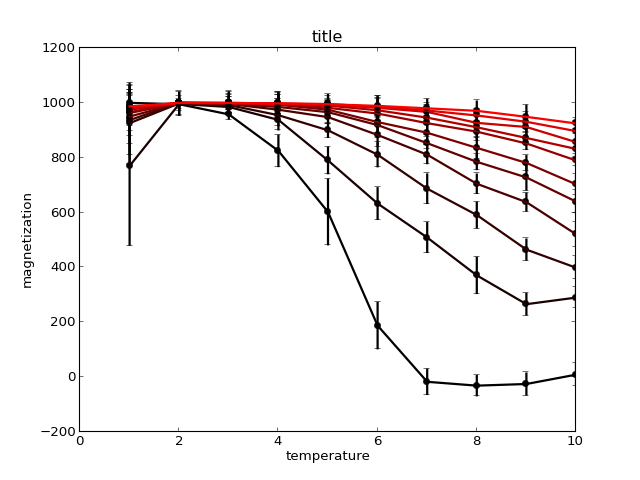
\includegraphics[width=4in]{images/ising.png}
\caption{Average magnetization as a function of the temperature for a spin system.\label{ising-mag}}
\end{figure}

Fig.~\ref{ising-state} shows the two-dimensional section of some random three-dimensional states for different values of the temperature. One can clearly see that the lower the temperature, the more the spins are aligned, and the higher the temperature, the more random they are.

\begin{figure}[ht]
\centering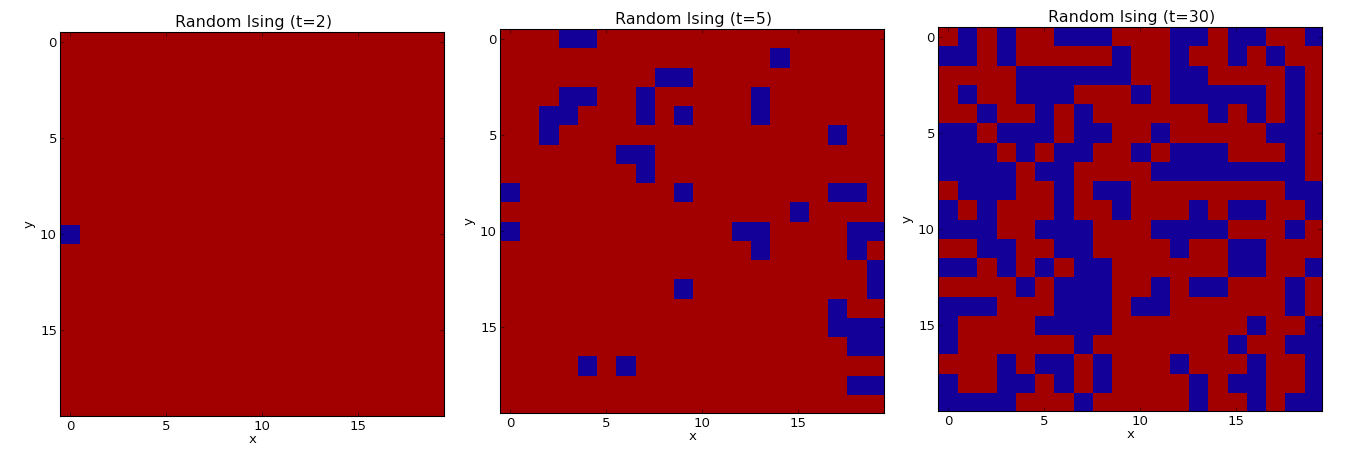
\includegraphics[width=4in]{images/ising2.png}
\caption{Random Ising states (2D section of 3D) for different temperatures.\label{ising-state}}
\end{figure}

\section{Simulated annealing}
\index{simulate annealing}\index{protein folding}

Simulated annealing is an application of Monte Carlo to solve optimization problems. It is best understood within the context of the Ising model. When the temperature is lowered, the system tends toward the state of minimum energy. At high temperature, the system fluctuates randomly and moves in the space of all possible states. This behavior is not specific to the Ising model. Hence, for any system for which we can define an energy, we can find its minimum energy state, by starting in a random state and slowly lowering the temperature as we evolve the simulation. The system will find a minimum. There may be more than one minimum, and one may need to repeat the procedure multiple times from different initial random states and compare the solutions. This process takes the name of annealing in analogy with the industrial process for removing impurities from metals: heat, cool slowly, repeat.

We can apply this process to any system for which we want to minimize a function $f(x)$ of multiple variables. We just have to think of $x$ as the state $s$ and of $f$ as the energy $E$. This analogy is purely semantic because the quantity we want to minimize is not necessarily an energy in the physical sense.

Simulated annealing does not assume the function is differentiable or continuous in its variables.

\subsection{Protein folding}

In the following we apply simulated annealing to the problem of folding of a protein.
A protein is a sequence of amino-acids. It is normally unfolded, and amino-acids are on a line. When placed in water, it folds. This is because some amino-acids are hydrophobic (repel water) and some are hydrophilic (like contact with water), therefore the protein tries to acquire a three-dimensional shape that minimizes the surface of hydrophobic amino-acids in contact with water~\cite{folding}. This is represented graphically in fig.~\ref{folding}.

\begin{figure}[ht]
\centering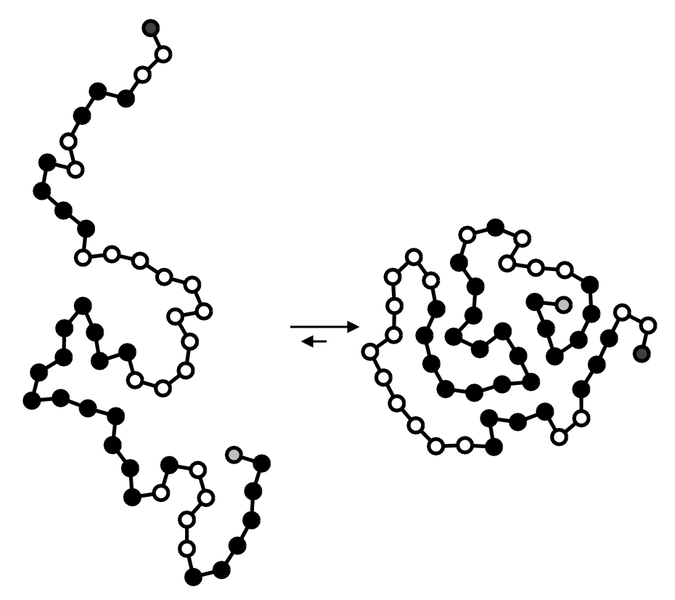
\includegraphics[width=2in]{images/folding.png}
\caption{Schematic example of protein folding. The white circles are hydrophilic amino-acids. The black ones are hydrophobic.\label{folding}}
\end{figure}

Here we assume only two types of amino-acids (H for hydrophobic and P for hydrophilic), and we assume each amino acid is a cube, that all cubes have the same size, and that each two consecutive amino-acids are connected at a face. These assumptions greatly simplify the problem because they limit the possible solid angles to six possible values (0: up, 1: down, 2: right, 3: left, 4: front, 5: back). Our goal is arranging the cubes to minimize the number of faces of hydrophobic cubes that are exposed to water:

\index{protein folding}\index{class!Protein}

%%% META:FILE:folding.nim
\begin{lstlisting}[caption={in file: {\ft folding.nim}}]
import nlib, std/random, std/math, std/tables

type
  Cell = (int, int, int)
  Protein* = ref object
    aminoacids*: string
    angles*: seq[int]
    folding*: Table[Cell, char]
    energy*: int

proc move(angle: int, c: Cell): Cell =
  case angle
  of 0: (c[0]+1, c[1], c[2])
  of 1: (c[0]-1, c[1], c[2])
  of 2: (c[0], c[1]+1, c[2])
  of 3: (c[0], c[1]-1, c[2])
  of 4: (c[0], c[1], c[2]+1)
  of 5: (c[0], c[1], c[2]-1)
  else: c

proc computeFolding(p: Protein, angles: seq[int]): Table[Cell, char] =
  var c: Cell = (0, 0, 0)
  var k = 0
  result[c] = p.aminoacids[k]
  for angle in angles:
    inc k
    let nxt = move(angle, c)
    if nxt in result: return initTable[Cell, char]()
    result[nxt] = p.aminoacids[k]
    c = nxt

proc computeEnergy(p: Protein, folding: Table[Cell, char]): int =
  for c, aa in folding:
    if aa == 'H':
      for face in 0 ..< 6:
        if not (move(face, c) in folding):
          inc result

proc newProtein*(aminoacids: string): Protein =
  result = Protein(
    aminoacids: aminoacids,
    angles: newSeq[int](aminoacids.len - 1))
  result.folding = result.computeFolding(result.angles)
  result.energy = result.computeEnergy(result.folding)

proc fold*(p: Protein, t: float): int =
  var newAngles: seq[int]
  var newFolding: Table[Cell, char]
  while true:
    newAngles = p.angles
    let n = rand(1 .. p.aminoacids.len - 2)
    newAngles[n] = rand(0 .. 5)
    newFolding = p.computeFolding(newAngles)
    if newFolding.len > 0: break
  let newEnergy = p.computeEnergy(newFolding)
  if float(p.energy - newEnergy) > t * ln(rand(1.0)):
    p.angles = newAngles
    p.folding = newFolding
    p.energy = newEnergy
  p.energy

proc main() =
  randomize()
  var aas = ""
  for _ in 0 ..< 20:
    aas.add (if rand(1.0) < 0.5: 'H' else: 'P')
  let protein = newProtein(aas)
  var t = 10.0
  while t > 1e-5:
    discard protein.fold(t)
    echo protein.energy, " ", protein.angles
    t *= 0.99

main()
\end{lstlisting}

The {\ft moves} dictionary is a dictionary of functions. For each solid angle (0--5), {\ft moves[angle]} is a function that maps {\ft x, y, z}, the coordinates of an amino acid, to the coordinates of the cube at that solid angle.

The annealing procedure is performed in the {\ft main} function. The {\ft fold} procedure is the same step as the Metropolis step. The purpose of the {\ft while} loop in the {\ft fold} function is to find a valid fold for the accept--reject step. Some folds are invalid because they are not physical and would require two amino-acids to occupy the same portion of space. When this happens, the {\ft compute\_folding} method returns {\ft None}, indicating that one must try a different folding.

\chapter{Parallel Algorithms}
\index{parallel algorithms}

Consider a program that performs the following computation:
\begin{lstlisting}
y = f(x)
z = g(x)
\end{lstlisting}
In this example, the function $g(x)$ does not depend on the result of the function $f(x)$, and therefore the two functions could be computed independently and in parallel.

Often large problems can be divided into smaller computational problems, which can be solved concurrently (``in parallel'') using different processing units (CPUs, cores). This is called {\it parallel computing}. Algorithms designed to work in parallel are called {\it parallel algorithms}.

In this chapter, we will refer to a processing unit as a node and to the code running on a node as a process. A parallel program consists of many processes running on as many nodes. It is possible for multiple processes to run on one and the same computing unit (node) because of the multitasking capabilities of modern CPUs, but that is not true parallel computing. We will use an emulator, {\ft PSim}, which does exactly that.

Programs can be parallelized at many levels: bit level, instruction level, data, and task parallelism. Bit-level parallelism is usually implemented in hardware. Instruction-level parallelism is also implemented in hardware in modern multi-pipeline CPUs.  Data parallelism is usually referred to as SIMD. Task parallelism is also referred to as MIMD.

Historically, parallelism was found in applications in high-performance computing, but today it is employed in many devices, including common cell phones. The reason is heat dissipation. It is getting harder and harder to improve speed by increasing CPU frequency because there is a physical limit to how much we can cool the CPU. So the recent trend is keeping frequency constant and increasing the number of processing units on the same chip.

Parallel architectures are classified according to the level at which the hardware supports parallelism, with multicore and multiprocessor computers having multiple processing elements within a single machine, while clusters, MPPs, and grids use multiple computers to work on the same task. Specialized parallel computer architectures are sometimes used alongside traditional processors for accelerating specific tasks.

Optimizing an algorithm to run on a parallel architecture is not an easy task. Details depend on the type of parallelism and details of the architecture.

In this chapter, we will learn how to classify architectures, compute running times of parallel algorithms, and measure their performance and scaling.

We will learn how to write parallel programs using standard programming patterns, and we will use them as building blocks for more complex algorithms.

For some parts of this chapter, we will use a simulator called {\ft PSim}, written in Nim on top of {\ft std/threadpool} and {\ft std/locks}. Its performance will only scale on multicore machines, but it allows us to emulate various network topologies on a single host.

\section{Parallel architectures}

\goodbreak\subsection{Flynn taxonomy}

\index{parallel architectures}\index{Flynn classification}\index{SISD}\index{SIMD}\index{MIMD}


Parallel computer architecture classifications are known as Flynn"s taxonomy~\cite{flynn} and are due to the work of Michael J. Flynn in 1966.

Flynn identified the following architectures:

\begin{itemize}
\item {\bf Single instruction, single data stream (SISD)}

A sequential computer that exploits no parallelism in either the instruction or data streams. A single control unit (CU) fetches a single instruction stream (IS) from memory. The CU then generates appropriate control signals to direct single processing elements (PE) to operate on a single data stream (DS), for example, one operation at a time.

Examples of SISD architecture are the traditional uniprocessor machines like a PC (currently manufactured PCs have multiple processors) or old mainframes.

\item {\bf Single instruction, multiple data streams (SIMD)}
A  computer  that   exploits   multiple  data   streams   against  a  single instruction stream  to perform operations that  may be naturally parallelized (e.g., an array processor or GPU).

\item {\bf Multiple instruction, single data stream (MISD)}

Multiple instructions operate on a single data stream. This is an uncommon architecture that is generally used for fault tolerance. Heterogeneous systems operate on the same data stream and must agree on the result. Examples include the now retired Space Shuttle flight control computer.

\item {\bf Multiple instruction, multiple data streams (MIMD)}
Multiple autonomous processors simultaneously executing different instructions on different data. Distributed systems are generally recognized to be MIMD architectures, either exploiting a single shared memory space (using threads) or a distributed memory space (using a message-passing protocol such as MPI).
\end{itemize}

\index{SPMD}\index{MPMD}

MIMD can be further subdivided into the following:
\begin{itemize}

\item {\bf Single program, multiple data (SPMD)}
Multiple autonomous processors simultaneously executing the same program but at independent points not synchronously (as in the SIMD case). SPMD is the most common style of parallel programming.

\item {\bf Multiple program, multiple data (MPMD)}
Multiple autonomous processors simultaneously operating at least two independent programs. Typically such systems pick one node to be the ``host'' (``the explicit host/node programming model'') or ``manager'' (the ``manager--worker'' strategy), which runs one program that farms out data to all the other nodes, which all run a second program. Those other nodes then return their results directly to the manager. The Map-Reduce pattern also falls under this category.
\end{itemize}

An embarrassingly parallel workload (or embarrassingly parallel problem) is one for which little or no effort is required to separate the problem into a number of parallel tasks. This is often the case where there exists no dependency (or communication) between those parallel tasks.

The manager--worker node strategy, when workers do not need to communicate with each other, is an example of an ``embarrassingly parallel'' problem.


\goodbreak\subsection{Network topologies}

\index{network topologies}\index{switch network}\index{bus network}\index{mesh network}\index{hypercube network}\index{tree network}

In the MIMD case, multiple copies of the same problem run concurrently (on different data subsets and branching differently, thus performing different instructions) on different processing units, and they exchange information using a network. How fast they can communicate depends on the network characteristics identified by the network topology and the latency and bandwidth of the individual links of the network.

Normally we classify network topologies based on the following taxonomy:

\begin{itemize}
\item {\bf Completely connected:}
Each node is connected by a directed link to each other node.
\item {\bf Bus topology:}
All nodes are connected to the same single cable. Each computer can therefore communicate with each other computer using one and the same bus cable. The limitation of this approach is that the communication bandwidth is limited by the bandwidth of the cable. Most bus networks only allow two machines to communicate with each other at one time (with the exception of one too many broadcast messages). While two machines communicate, the others are stuck waiting.
The bus topology is the most inexpensive but also slow and constitutes a single point of failure.
\item {\bf Switch topology (star topology):}
In local area networks with a switch topology, each computer is connected via a direct link to a central device, usually a switch, and it resembles a star. Two computers can communicate using two links (to the switch and from the switch). The central point of failure is the switch. The switch is usually intelligent and can reroute the messages from any computer to any other computer. If the switch has sufficient bandwidth, it can allow multiple computers to talk to each other at the same time. For example, for a 10 Gbit/s links and an 80 Gbit/s switch, eight computers can talk to each other (in pairs) at the same time.
\item {\bf Mesh topology:}
In a mesh topology, computers are assembled into an array (1D, 2D, etc.), and each computer is connected via a direct link to the computers immediately close (left, right, above, below, etc.). Next neighbor communication is very fast because it involves a single link and therefore low latency. For two computers not physically close to communicate, it is necessary to reroute messages. The latency is proportional to the distance in links between the computers. Some meshes do not support this kind of rerouting because the extra logic, even if unused, may be cause for extra latency. Meshes are ideal for solving numerical problems such as solving differential equations because they can be naturally mapped into this kind of topology.
\item {\bf Torus topology:}
Very similar to a mesh topology (1D, 2D, 3D, etc.), except that the network wraps around the edges. For example, in one dimension node, $i$ is connected to $(i+1) \% p$, where $p$ is the total number of nodes. A one-dimensional torus is called a {\it ring network}.
\item {\bf Tree network:}
The tree topology looks like a tree where the computer may be associated with every tree node or every leaf only. The tree links are the communication link. For a binary tree, each computer only talks to its parent and its two children nodes. The root node is special because it has no parent node.

Tree networks are ideal for global operations such as broadcasting and for sharing IO devices such as disks. If the IO device is connected to the root node, every other computer can communicate with it using only $\log p$ links (where $p$ is the number of computers connected). Moreover, each subset of a tree network is also a tree network. This makes it easy to distribute subtasks to different subsets of the same architecture.

\item{\bf Hypercube:}
This network assumes $2^d$ nodes, and each node corresponds to a vertex of a hypercube. Nodes are connected by direct links, which correspond to the edges of the hypercube. Its importance is more academic than practical, although some ideas from hypercube networks are implemented in some algorithms.
\end{itemize}

If we identify each node on the network with a unique integer number called its rank, we write explicit code to determine if two nodes $i$ and $j$ are connected for each network topology:

\index{PSim emulator}

%%% META:FILE:psim.nim
\begin{lstlisting}[caption={in file: {\ft psim.nim}}]
import std/math

type Topology* = proc(i, j: int): bool

proc BUS*(): Topology = (proc(i, j: int): bool = true)
proc SWITCH*(): Topology = (proc(i, j: int): bool = true)

proc MESH1*(p: int): Topology =
  result = proc(i, j: int): bool = (i - j) * (i - j) == 1

proc TORUS1*(p: int): Topology =
  result = proc(i, j: int): bool =
    ((i - j + p) mod p == 1) or ((j - i + p) mod p == 1)

proc MESH2*(p: int): Topology =
  let q = int(sqrt(float(p)) + 0.1)
  result = proc(i, j: int): bool =
    let dx = (i mod q - j mod q) * (i mod q - j mod q)
    let dy = (i div q - j div q) * (i div q - j div q)
    (dx, dy) in [(1, 0), (0, 1)]

proc TORUS2*(p: int): Topology =
  let q = int(sqrt(float(p)) + 0.1)
  result = proc(i, j: int): bool =
    ((i mod q - j mod q + q) mod q,
     (i div q - j div q + q) mod q) in [(0, 1), (1, 0)] or
    ((j mod q - i mod q + q) mod q,
     (j div q - i div q + q) mod q) in [(0, 1), (1, 0)]

proc TREE*(): Topology =
  result = proc(i, j: int): bool =
    i == (j - 1) div 2 or j == (i - 1) div 2
\end{lstlisting}

\goodbreak\subsection{Network characteristics}

\index{diameter of network}\index{bisection width}\index{arc connectivity}

\begin{itemize}
\item {\bf Number of links}

\item {\bf Diameter:} The max distance between any two nodes measured as a minimum number of links connecting them. Smaller diameter means smaller latency. The diameter is proportional to the maximum time it takes for a message go from one node to another.

\item {\bf Bisection width:} The minimum number of links one has to cut to turn the network into two disjoint networks. Higher bisection width means higher reliability of the network.

\item {\bf Arc connectivity:} The number of different paths (non-overlapping and of minimal length) connecting any two nodes. Higher connectivity means higher bandwidth and higher reliability.
\end{itemize}

Here are values of this parameter for each type of network:

\begin{tabular}{|l|lll|} \hline
Network              & Links & Diameter & Width \\ \hline
completely connected & $p(p-1)/2$   & $1$   & $p-1$ \\
switch               & $p$          & $2$   & $1$ \\
1D mesh              & $p-1$        & $p-1$ & $1$ \\
nD mesh              & $n(p^{\frac1n}-1)p^{\frac{n-1}n}$ & $n$ & $p^{\frac23}$ \\
1D torus             & $p$          & $\frac{p}2$ & $2$ \\
nD torus             & $np$         & $\frac{n}2 p^{\frac1n}$ & $2n$ \\
hypercube            & $\frac{p}2 \log_2 p$ & $\log_2 p$ & $log_2 p$ \\
tree                 & $p-1$        & $\log_2 p$ & $1$ \\ \hline
\end{tabular}

\begin{figure}[ht]
\centering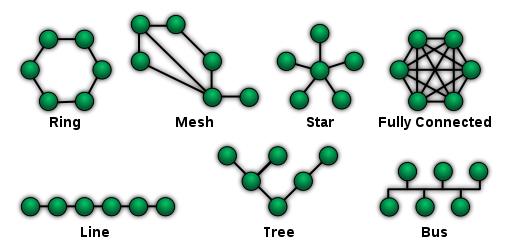
\includegraphics[width=4in]{images/network_topologies.png}
\caption{Examples of network topologies.}
\end{figure}

Most actual supercomputers implement a variety of taxonomies and topologies simultaneously. A modern supercomputer has many nodes, each node has many CPUs, each CPU has many cores, and each core implements SIMD instructions. Each core has it own cache, each CPU has its own cache, and each node has its own memory shared by all threads running on that one node. Nodes communicate with each other using multiple networks (typically a multidimensional mesh for point-to-point communications and a tree network for global communication and general disk IO).

This makes writing parallel programs very difficult. Parallel programs must be optimized for each specific architecture.

\goodbreak\section{Parallel metrics}

\goodbreak\subsection{Latency and bandwidth}

\index{latency}\index{bandwidth}

The time it takes for a message of size $m$ (in bytes) over a wire can be broken into two components: a fixed overall time that does not depend on the size of the message, called {\it latency} (and indicated with $t_s$), and a time proportional to the message size, called {\it inverse bandwidth} (and indicated with $t_w$).

Think of a pipe of length $L$ and section $s$, and you want to pump $m$ liters of water through the pipe at velocity $v$. From the moment you start pumping, it takes $L/v$ seconds before the water starts arriving at the other end of the pipe. From that moment, it will take $m / sv$ for all the water to arrive at its destination. In this analogy, $L/v$ is the latency $t_s$, $sv$ is the bandwidth, and $t_w = 1/sv$.

The total time to send the message (or the water) is

\begin{equation}
T(m) = t_s + t_w m
\end{equation}

From now on, we will use $T_1(n)$ to refer to the nonparallel running time of an algorithm as a function of its input $m$. We will use $T_p(n)$ to refer to its running time with $p$ parallel processes.

As a practical case, in the following example, we consider a generic algorithm with the following parallel and nonparallel running times:

\begin{eqnarray}
T_1(n) &=& t_a n^2 \\
T_p(n) &=& t_a n^2 / p + 2p (t_s+t_w n/p)
\end{eqnarray}

These formulas may come for example from the problem of multiplying a matrix times a vector.

Here $t_a$ is the time to perform one elementary instruction; $t_s$ and $t_w$ are the latency and inverse bandwidth. The first term of $T_p$ is nothing but $T_1/p$, while the second term is an overhead due to communications.

Typically $t_s >> t_w >> t_a$. In the following plots, we will always assume $t_a=1$, $t_s=0.2$, and $t_w=0.1$. With these assumptions, fig.~\ref{Tp} shows how $T_p$ changes with input size and number of parallel processes. Notice that while for small $p$, $T_p$ decreases $\propto 1/p$, for large $p$, the communication overhead dominates over computation. This overhead is our example and is dominated by the latency contribution, which grows with $p$.

\begin{figure}[ht]
\centering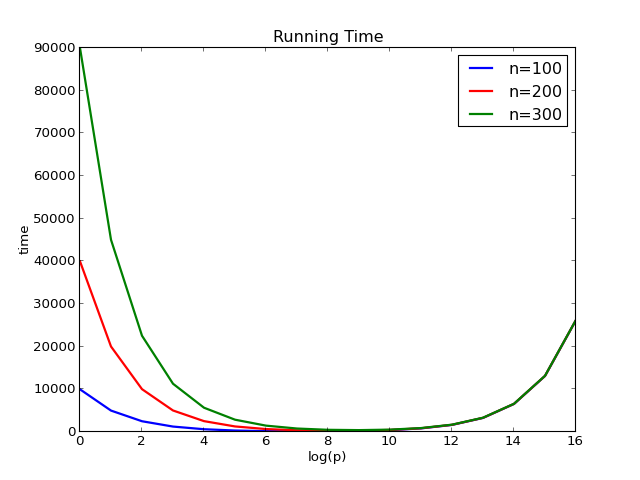
\includegraphics[width=4in]{images/Tp.png}
\caption{$T_p$ as a function of input size $n$ and number of processes $p$.\label{Tp}}
\end{figure}

\goodbreak\subsection{Speedup}\index{speedup}

The {\it speedup} is defined as

\begin{equation}
S_p(n) = \frac{T_1(n)}{T_p(n)}
\end{equation}
where $T_1$ is the time it takes to run the algorithm on an input of size $n$ on one processing unit (e.g., node), and $T_p$ is the time it takes to run the same algorithm on the same input using $p$ nodes in parallel. Fig.~\ref{Sp} shows an example of speedup. When communication overhead dominates, speedup decreases.

\begin{figure}[ht]
\centering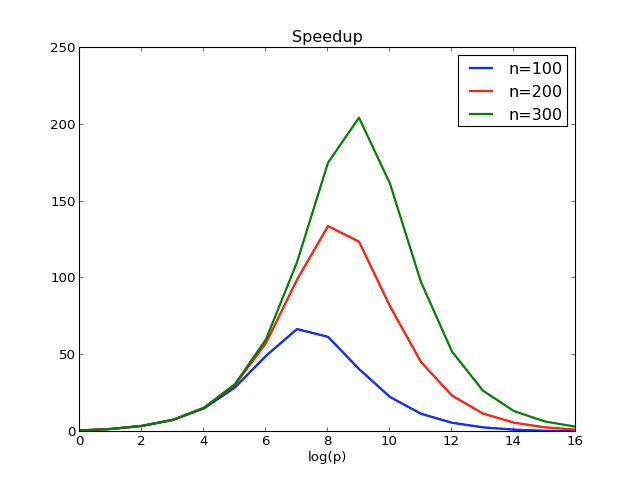
\includegraphics[width=4in]{images/Sp.png}
\caption{$S_p$ as a function of input size $n$ and number of processes $p$.\label{Sp}}
\end{figure}

\goodbreak\subsection{Efficiency}\index{efficiency}

The {\it efficiency} is defined as

\begin{equation}
E_p(n) = \frac{S_p(n)}{p} = \frac{T_1(n)}{p T_p(n)}
\end{equation}
Notice that in case of perfect parallelization (impossible), $T_p=T_1/p$, and therefore $E_p(n)=1$. Fig.~\ref{Ep} shows an example of efficiency. When communication overhead dominates, efficiency drops. Notice efficiency is always less than 1. We do not write parallel algorithms because they are more efficient. They are always less efficient and more costly than the nonparallel ones. We do it because we want the result sooner, and there is an economic value in it.

\begin{figure}[ht]
\centering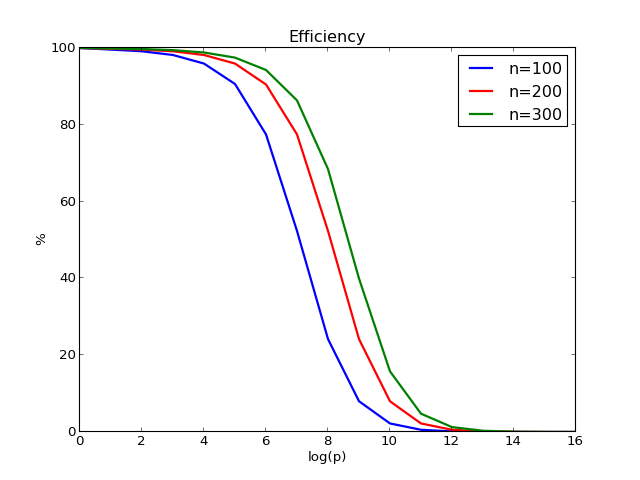
\includegraphics[width=4in]{images/Ep.png}
\caption{$E_p$ as a function of input size $n$ and number of processes $p$.\label{Ep}}
\end{figure}

\goodbreak\subsection{Isoefficiency}\index{isoefficiency}

Given a value of efficiency that we choose as target, $E$, and a given number of nodes, $p$, we ask what is the maximum size of a problem that we can solve. The answer is found by solving for $n$ the following equation:

\begin{equation}
E_p(n) = E
\end{equation}
For example $T_p$, we obtain
\begin{equation}
E_p = \frac1{1 + 2p^2(t_s + t_w n/p)/(n^2 t_a)} = E
\end{equation}
which solved in $n$ yields
\begin{equation}
n \simeq 2 \frac{t_w}{t_a} \frac{E}{1-E} p
\end{equation}
Isoefficiency curves for different values of $E$ are shown in fig.~\ref{Ip}.
For our example problem, $n$ is proportional to $p$. In general, this is not true, but $n$ is monotonic in $p$.

\begin{figure}[ht]
\centering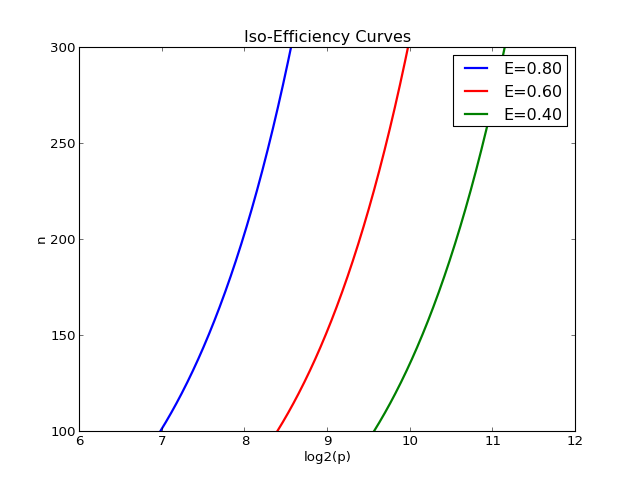
\includegraphics[width=4in]{images/Ip.png}
\caption{Isoefficiency curves for different values of the target efficiency.\label{Ip}}
\end{figure}

\goodbreak\subsection{Cost}\index{cost of computation}

The cost of a computation is equal to the time it takes to run on each node, multiplied by the number of nodes involved in the computation:

\begin{equation}
C_p(n) = p T_p(n)
\end{equation}

Notice that in general

\begin{equation}
\frac{\textrm{d}C_p(n)}{\textrm{d}p} = \alpha T_1(n) > 0
\end{equation}

This means that for a fixed problem size $n$, the more an algorithm is parallelized, the more it costs to run it (because it gets less and less efficient).

\begin{figure}[ht]
\centering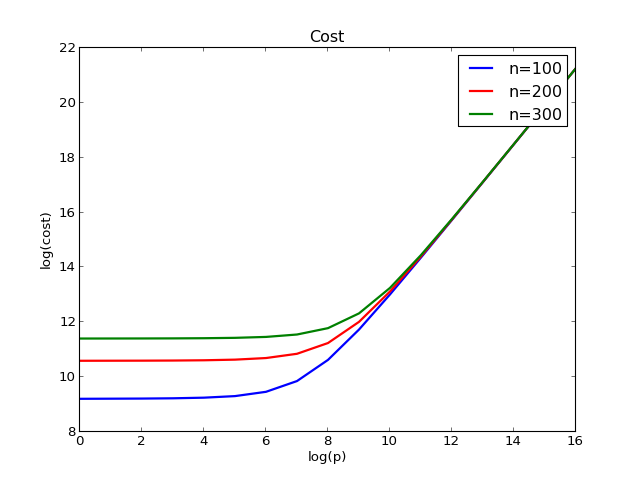
\includegraphics[width=4in]{images/Cp.png}
\caption{$C_p$ as a function of input size $n$ and a number of processes $p$.\label{Cp}}
\end{figure}

\goodbreak\subsection{Cost optimality}\index{cost optimality}

With the preceding disclaimer, we define cost optimality as the choice of $p$ (as a function of $n$), which makes the cost scale proportional to $T_1(n)$:

\begin{equation}
p T_p(n) \propto T_1(n)
\end{equation}

Or in other words, looking for the $p(n)$ such that

\begin{equation}
\lim_{n\rightarrow\infty} p(n) T_{p(n)}(n) / T_1(n) = const. \ne 0
\end{equation}

\goodbreak\subsection{Amdahl"s law}\index{Amdahl"s law}

Consider an algorithm that can be parallelized, but one fraction $\alpha$ of its total sequential running time $\alpha T_1$ cannot be parallelized. That means that $T_p = \alpha T_1 + (1-\alpha) T_1/p$, and this yields~\cite{admhal}

\begin{equation}
S_p = \frac{1}{\alpha+(1-\alpha)/p} < \frac{1}{\alpha}
\end{equation}

Therefore the speedup is theoretically limited.

\goodbreak\section{Message passing}\index{message passing}

Consider the following Nim program:
\begin{lstlisting}
import std/posix

proc f() =
  if fork() != 0:
    echo true
  else:
    echo false
f()
\end{lstlisting}
The output of the current program is
\begin{lstlisting}
true
false
\end{lstlisting}

{\ft fork} (from {\ft std/posix}) creates a copy of the current process (a child). The parent gets the child's PID; the child gets 0. So the {\ft if} branches both ways, on different processes.

The source of {\ft PSim} is included in the {\ft psim.nim} file.

\index{PSim emulator}\index{class!PSim}\index{send}\index{recv}\index{point-to-point}

%%% META:FILE:psim.nim
\begin{lstlisting}[caption={in file: {\ft psim.nim}}]
import std/[json, threadpool, locks]

type
  PSim* = ref object
    nprocs*, rank*: int
    topology*: Topology
    pipes*: seq[seq[Channel[string]]]
    logFile*: File

proc newPSim*(p: int, topology = SWITCH(),
              logFilename = ""): PSim =
  ## Spawns `p-1` worker threads via `std/threadpool` and creates one
  ## `Channel[string]` per (sender, receiver) pair; messages are
  ## serialized via JSON so any value type can flow through a channel.
  result = PSim(nprocs: p, topology: topology, rank: 0)
  result.pipes = newSeq[seq[Channel[string]]](p)
  for i in 0 ..< p:
    result.pipes[i] = newSeq[Channel[string]](p)
    for j in 0 ..< p:
      result.pipes[i][j].open()
  if logFilename.len > 0:
    result.logFile = open(logFilename, fmWrite)

proc log*(s: PSim, message: string) =
  if not s.logFile.isNil: s.logFile.write(message)

proc privateSend*[T](s: PSim, j: int, data: T) =
  if j < 0 or j >= s.nprocs:
    raise newException(IOError, "send: invalid rank")
  s.pipes[s.rank][j].send($ %*data)

proc send*[T](s: PSim, j: int, data: T) =
  if not s.topology(s.rank, j):
    raise newException(IOError, "topology violation")
  s.privateSend(j, data)

proc privateRecv*[T](s: PSim, j: int, _: typedesc[T]): T =
  if j < 0 or j >= s.nprocs:
    raise newException(IOError, "recv: invalid rank")
  let raw = s.pipes[j][s.rank].recv()
  to(parseJson(raw), T)

proc recv*[T](s: PSim, j: int, t: typedesc[T]): T =
  if not s.topology(s.rank, j):
    raise newException(IOError, "topology violation")
  s.privateRecv(j, t)
\end{lstlisting}

\index{communicator}

An instance of the class {\ft PSim} is an object that can be used to determine the total number of parallel processes, the rank of each running process, to send messages to other processes, and to receive messages from them. It is usually called a {\it communicator}; {\ft send} and {\ft recv} represent the simplest type of communication pattern, point-to-point communication.

A PSim program starts by importing and creating an instance of the {\ft PSim} class. The constructor takes two arguments, the number of parallel processes you want and the network topology you want to emulate. Before returning the {\ft PSim} instance, the constructor makes $p-1$ copies of the running process and creates sockets connecting each two of them. Here is a simple example in which we make two parallel processes and send a message from process 0 to process 1:

\begin{lstlisting}
import psim

let comm = newPSim(2, SWITCH())
if comm.rank == 0:
  comm.send(1, "Hello World")
elif comm.rank == 1:
  let message = comm.recv(0, string)
  echo message
\end{lstlisting}

Here is a more complex example that creates $p=10$ parallel processes, and node 0 sends a message to each one of them:


\begin{lstlisting}
import psim

const p = 10
let comm = newPSim(p, SWITCH())
if comm.rank == 0:
  for other in 1 ..< p:
    comm.send(other, "Hello " & $p)
else:
  let message = comm.recv(0, string)
  echo message
\end{lstlisting}

 Following is a more complex example that implements a parallel scalar product. The process with rank 0 makes up two vectors and distributes pieces of them to the other processes. Each process computes a part of the scalar product. Of course, the scalar product runs in linear time, and it is very inefficient to parallelize it, yet we do it for didactic purposes.

\index{parallel!scalar product}

%%% META:FILE:psim_scalar.nim
\begin{lstlisting}[caption={in file: {\ft psim\_scalar.nim}}]
import psim, std/random

proc scalarProductTest1(n, p: int) =
  let comm = newPSim(p)
  let h = n div p
  var a, b: seq[float]
  if comm.rank == 0:
    randomize()
    for _ in 0 ..< n: a.add rand(1.0)
    for _ in 0 ..< n: b.add rand(1.0)
    for k in 1 ..< p:
      comm.send(k, a[k*h ..< k*h + h])
      comm.send(k, b[k*h ..< k*h + h])
  else:
    a = comm.recv(0, seq[float])
    b = comm.recv(0, seq[float])
  var scalar = 0.0
  for i in 0 ..< h: scalar += a[i] * b[i]
  if comm.rank == 0:
    for k in 1 ..< p: scalar += comm.recv(k, float)
    echo scalar
  else:
    comm.send(0, scalar)

scalarProductTest1(10, 2)
\end{lstlisting}

Most parallel algorithms follow a similar pattern. One process has access to IO. That process reads and scatters the data. The other processes perform their part of the computation; the results are reduced (aggregated) and sent back to the root process. This pattern may be repeated by multiple functions, perhaps in loops. Different functions may handle different data structure and may have different communication patterns. The one thing that must be constant throughout the run is the number of processes because one wants to pair each process with one computing unit.

 In the following, we implement a parallel version of the {\ft mergesort}. At each step, the code splits the problem into two smaller problems. Half of the problem is solved by the process that performed the split and assigns the other half to an existing free process. When there are no more free processes, it reverts to the nonparallel {\ft mergesort} step. The {\ft merge} function here is the same as the nonparallel {\ft mergesort} of chapter 3.

\index{mergesort!parallel}

%%% META:FILE:psim_mergesort.nim
\begin{lstlisting}[caption={in file: {\ft psim\_mergesort.nim}}]
import psim, nlib, std/random
# `merge` and `mergesort` are reused from nlib (chapter 3).

proc mergesortTest(n, p: int) =
  let comm = newPSim(p)
  if comm.rank == 0:
    randomize()
    var data: seq[float]
    for _ in 0 ..< n: data.add rand(1.0)
    comm.send(1, data[n div 2 .. ^1])
    mergesort(data, 0, n div 2)
    let other = comm.recv(1, seq[float])
    for i, v in other:
      data[n div 2 + i] = v
    merge(data, 0, n div 2, n)
    echo data
  else:
    var data = comm.recv(0, seq[float])
    mergesort(data)
    comm.send(0, data)

mergesortTest(20, 2)
\end{lstlisting}

More interesting patterns are global communication patterns implemented on top of {\ft send} and {\ft recv}. Subsequently, we discuss the most common: broadcast, scatter, collect, and reduce. Our implementation is not the most efficient, but it is the simplest. In principle, there should be a different implementation for each type of network topology to take advantage of its features.


\goodbreak\subsection{Broadcast}\index{broadcast}

The simplest type of broadcast is the one-2-all, which consists of one process (source) sending a message (value) to every other process. A more complex broadcast is when each process broadcasts a message simultaneously and each node receives the list of values ordered by the rank of the sender:

%%% META:FILE:psim.nim
\begin{lstlisting}[caption={in file: {\ft psim.nim}}]
proc one2allBroadcast*[T](s: PSim, source: int, value: T): T =
  if s.rank == source:
    for i in 0 ..< s.nprocs:
      if i != source:
        s.privateSend(i, value)
    result = value
  else:
    result = s.privateRecv(source, T)

proc all2oneCollect*[T](s: PSim, destination: int, value: T): seq[T]
proc all2allBroadcast*[T](s: PSim, value: T): seq[T] =
  var vector = s.all2oneCollect(0, value)
  vector = s.one2allBroadcast(0, vector)
  vector
\end{lstlisting}

We have implemented the all-to-all broadcast using a trick. We collected all values and sent them to the node with rank 0 (via a function collect), and then we did a one-to-all broadcast of the entire list from node 0. In general, the implementation depends on the topology of the available network.

Here is an example of an application of broadcasting:

\begin{lstlisting}
import psim

const p = 10
let comm = newPSim(p, SWITCH())
var message = if comm.rank == 0: "Hello World" else: ""
message = comm.one2allBroadcast(0, message)
echo message
\end{lstlisting}

Notice how before the broadcast, only the process with rank 0 has knowledge of the message. After broadcast, all nodes are aware of it. Also notice that {\ft one2all\_broadcast} is a global communication function, and all processes must call it. Its first argument is the rank of the broadcasting process (0), while the second argument is the message to be broadcasted (only the value from node 0 is actually used).

\goodbreak\subsection{Scatter and collect}\index{scatter}\index{collect}

The all-to-one collect pattern works as follows. Every process sends a value to process {\ft destination}, which receives the values in a list ordered according to the rank of the senders:

%%% META:FILE:psim.nim
\begin{lstlisting}[caption={in file: {\ft psim.nim}}]
proc one2allScatter*[T](s: PSim, source: int,
                        data: seq[T]): seq[T] =
  if s.rank == source:
    var h = data.len div s.nprocs
    if data.len mod s.nprocs != 0: h += 1
    for i in 0 ..< s.nprocs:
      s.privateSend(i, data[i * h ..< min(i * h + h, data.len)])
  result = s.privateRecv(source, seq[T])

proc all2oneCollect*[T](s: PSim, destination: int, value: T): seq[T] =
  s.privateSend(destination, value)
  if s.rank == destination:
    for i in 0 ..< s.nprocs:
      result.add s.privateRecv(i, T)
\end{lstlisting}

Here is a revised version of the previous scalar product example using scatter:

%%% META:FILE:psim_scalar2.nim
\begin{lstlisting}[caption={in file: {\ft psim\_scalar2.nim}}]
import psim, std/random

proc scalarProductTest2(n, p: int) =
  let comm = newPSim(p)
  var a, b: seq[float]
  if comm.rank == 0:
    randomize()
    for _ in 0 ..< n: a.add rand(1.0)
    for _ in 0 ..< n: b.add rand(1.0)
  a = comm.one2allScatter(0, a)
  b = comm.one2allScatter(0, b)
  var scalar = 0.0
  for i in 0 ..< a.len: scalar += a[i] * b[i]
  scalar = comm.all2oneReduce(0, scalar,
                               proc(x, y: float): float = x + y)
  if comm.rank == 0: echo scalar

scalarProductTest2(10, 2)
\end{lstlisting}

\goodbreak\subsection{Reduce}\index{reduce}

The all-to-one reduce pattern is very similar to the collect, except that the {\ft destination} does not receive the entire list of values but some aggregated information about the values. The aggregation must be performed using a commutative binary function $f(x, y)=f(y, x)$. This guarantees that the reduction from the values go down in any order and thus are optimized for different network topologies.

The all-to-all reduce is similar to reduce, but every process will get the result of the reduction, not just one {\ft destination} node. This may be achieved by an all-to-one reduce followed by a one-to-all broadcast:

%%% META:FILE:psim.nim
\begin{lstlisting}[caption={in file: {\ft psim.nim}}]
proc all2oneReduce*[T](s: PSim, destination: int, value: T,
                       op: proc(a, b: T): T): T =
  s.privateSend(destination, value)
  if s.rank == destination:
    result = s.privateRecv(0, T)
    for i in 1 ..< s.nprocs:
      result = op(result, s.privateRecv(i, T))

proc all2allReduce*[T](s: PSim, value: T,
                       op: proc(a, b: T): T): T =
  result = s.all2oneReduce(0, value, op)
  result = s.one2allBroadcast(0, result)
\end{lstlisting}

And here are some examples of a reduce operation that can be passed to the {\ft op} argument of the {\ft all2one\_reduce} and {\ft all2all\_reduce} methods:

%%% META:FILE:psim.nim
\begin{lstlisting}[caption={in file: {\ft psim.nim}}]
proc psumOp*[T](x, y: T): T = x + y
proc pmulOp*[T](x, y: T): T = x * y
proc pmaxOp*[T](x, y: T): T = (if x > y: x else: y)
proc pminOp*[T](x, y: T): T = (if x < y: x else: y)
\end{lstlisting}

Graph algorithms can also be parallelized, for example, the Prim algorithm. One way to do it is to represent the graph using an adjacency matrix where term $i, j$ corresponds to the link between vertex $i$ and vertex $j$. The term can be {\ft None} if the link does not exist. Any graph algorithm, in some order, loops over the vertices and over the neighbors. This step can be parallelized by assigning different columns of the adjacency matrix to different computing processes. Each process only loops over some of the neighbors of the vertex being processed. Here is an example of the Prim algorithm:

%%% META:FILE:psim_prim.nim
\begin{lstlisting}[caption={in file: {\ft psim\_prim.nim}}]
import psim, std/random, std/sequtils

proc randomAdjacencyMatrix(n: int): seq[seq[int]] =
  result = newSeqWith(n, newSeq[int](n))
  for r in 0 ..< n:
    for c in 0 ..< r:
      let v = rand(1 .. 100)
      result[r][c] = v
      result[c][r] = v

type
  Vertex = object
    path: seq[int]

proc weight(path: seq[int], adjacency: seq[seq[int]]): int =
  for i in 1 ..< path.len:
    result += adjacency[path[i-1]][path[i]]

proc bb(adjacency: seq[seq[int]], p = 1): (seq[int], int) =
  let n = adjacency.len
  let comm = newPSim(p)
  var Q: seq[Vertex] = @[Vertex(path: @[0])]
  var bound = high(int)
  var optimal: seq[int] = @[]
  let localVertices = comm.one2allScatter(0, toSeq(0 ..< n))
  while true:
    var vertex: Vertex
    var sentinel = false
    if comm.rank == 0:
      if Q.len == 0:
        sentinel = true
      else:
        vertex = Q.pop()
    sentinel = comm.one2allBroadcast(0, sentinel)
    if sentinel: break
    vertex = comm.one2allBroadcast(0, vertex)
    var P: seq[Vertex] = @[]
    for k in localVertices:
      if k notin vertex.path:
        var newPath = vertex.path & k
        var newPathLength = weight(newPath, adjacency)
        if newPathLength < bound:
          if newPath.len == n:
            newPath.add newPath[0]
            newPathLength = weight(newPath, adjacency)
            if newPathLength < bound:
              bound = newPathLength
              optimal = newPath
          else:
            P.add Vertex(path: newPath)
        echo newPath, " ", newPathLength
    let x = comm.all2allReduce((bound, optimal),
              proc(a, b: (int, seq[int])): (int, seq[int]) =
                if a[0] < b[0]: a else: b)
    bound = x[0]
    optimal = x[1]
    let collected = comm.all2oneCollect(0, P)
    if comm.rank == 0:
      for batch in collected:
        for v in batch: Q.add v
  (optimal, bound)

let m = randomAdjacencyMatrix(5)
echo bb(m, p = 2)
\end{lstlisting}

\goodbreak\subsection{Barrier}\index{barrier}

Another global communication pattern is the barrier. It forces all processes when they reach the barrier to stop and wait until all the other processes have reached the barrier. Think of runners gathering at the  starting line  of a race; when  all the runners are there, the race can start.

Here we implement it using a simple all-to-all broadcast:

%%% META:FILE:psim.nim
\begin{lstlisting}[caption={in file: {\ft psim.nim}}]
proc barrier*(s: PSim) =
  discard s.all2allBroadcast(0)
\end{lstlisting}

The use of {\ft barrier} is usually a symptom of bad code because it forces parallel processes to wait for other processes without data actually being transferred.

\goodbreak\subsection{Global running times}

In the following table, we compute the order of growth or typical running times for the most common network topologies for typical communication algorithms:

\begin{tabular}{|l|lll|} \hline
Network & Send/Recv & One2All Bcast & Scatter \\ \hline
completely connected & $1$ & $1$ & $1$ \\
switch  & $2$ & $\log p$ & $2p$ \\
1D mesh  & $p-1$ & $p-1$ & $p^2$ \\
2D mesh  & $2(p^{\frac12}-1)$ & $\sqrt{p}$ & $p^2$ \\
3D mesh  & $3(p^{\frac13}-1)$ & $p^{1/3}$ & $p^2$ \\
1D torus  & $p/2$ & $p/2$ & $p^2$ \\
2D torus  & $2p^{\frac12}$ & $\sqrt{p}/2$ & $p^2$ \\
3D torus  & $3/2 p^{\frac13}$ & $p^{1/3}/2$ & $p^2$ \\
hypercube  & $\log p$ & $\log_2 p$ & $p$ \\
tree  & $\log p$ & $\log p$ & $p$
\\ \hline
\end{tabular}

It is obvious that the completely connected is the fastest network but also the most expensive to build. The tree is a cheap compromise. The switch tends to be faster for arbitrary point-to-point communication, but the switch comes to a premium. Multidimensional meshes and toruses become cost-effective when solving problems that are naturally defined on a grid because they only require next neighbor interaction.

\goodbreak\section{Master-Worker and Map-Reduce}\index{map-reduce}\index{master}\index{worker}\index{asynchat}\index{asyncore}

Map-Reduce~\cite{mapreduce} is a framework for processing highly distributable problems across huge data sets using a large number of computers (nodes). The group of computers is collectively referred to as a cluster (if all nodes use the same hardware) or a grid (if the nodes use different hardware). It comprises two steps:

``Map'' (implemented here in a function {\ft mapfn}): The master node takes the input data, partitions it into smaller subproblems, and distributes individual pieces of the data to worker nodes. A worker node may do this again in turn, leading to a multilevel tree structure. The worker node processes the smaller problem, computes a result, and passes that result back to its master node.

``Reduce'' (implemented here in a function {\ft reducefn}): The master node collects the partial results from all the subproblems and combines them in some way to compute the answer to the problem it needs.

Map-Reduce allows for distributed processing of the map and reduction operations. Provided each mapping operation is independent of the others, all maps can be performed in parallel---though in practice, it is limited by the number of independent data sources and/or the number of CPUs near each source. Similarly, a set of ``reducers'' can perform the reduction phase, provided all outputs of the map operation that share the same key are presented to the same reducer at the same time.

While this process can often appear inefficient compared to algorithms that are more sequential, Map-Reduce can be applied to significantly larger data sets than ``commodity'' servers can handle---a large server farm can use Map-Reduce to sort a petabyte of data in only a few hours, which would require much longer in a monolithic or single process system.

Parallelism also offers some possibility of recovering from partial failure of servers or storage during the operation: if one mapper or reducer fails, the work can be rescheduled---assuming the input data are still available.

Map-Reduce comprises two main functions: {\ft mapfn} and {\ft reducefn}. {\ft mapfn} takes a (key, value) pair of data with a type in one data domain and returns a list of (key, value) pairs in a different domain:
\begin{equation}
\textrm{mapfn}(k1, v1) \rightarrow (k2, v2)
\end{equation}
The {\ft mapfn} function is applied in parallel to every item in the input data set. This produces a list of (k2, v2) pairs for each call. After that, the Map-Reduce framework collects all pairs with the same key from all lists and groups them together, thus creating one group for each one of the different generated keys.
The {\ft reducefn} function is then applied in parallel to each group, which in turn produces a collection of values in the same domain:
\begin{equation}
\textrm{reducefn}(k2, [\textrm{list of }v2]) \rightarrow (k2, v3)
\end{equation}
The values returned by {\ft reducefn} are then collected into a single list. Each call to {\ft reducefn} can produce one, none, or multiple partial results.
Thus the Map-Reduce framework transforms a list of (key, value) pairs into a list of values.
It is necessary but not sufficient to have implementations of the map and reduce abstractions to implement Map-Reduce. Distributed implementations of Map-Reduce require a means of connecting the processes performing the {\ft mapfn} and {\ft reducefn} phases.

Here is a nonparallel implementation that explains the data workflow better:

%%% META:FILE:mapreduce.nim
\begin{lstlisting}[caption={in file: {\ft mapreduce.nim}}]
import std/tables

proc mapreduce*[T, K, V, R](
    mapper: proc(item: T): (K, V),
    reducer: proc(key: K, values: seq[V]): R,
    data: seq[T]): Table[K, R] =
  var partials = initTable[K, seq[V]]()
  for item in data:
    let (key, value) = mapper(item)
    if key notin partials:
      partials[key] = @[value]
    else:
      partials[key].add value
  for key, values in partials:
    result[key] = reducer(key, values)
\end{lstlisting}

And here is an example we can use to find how many random DNA strings contain the subsequence ``ACTA'':

\begin{lstlisting}
import std/[random, strutils]
randomize()
let bases = "ATGC"
var strings: seq[string]
for _ in 0 ..< 100:
  var s = ""
  for _ in 0 ..< 10: s.add bases[rand(bases.len - 1)]
  strings.add s

proc mapfn(s: string): (bool, int) = (("ACCA" in s), 1)
proc reducefn(check: bool, values: seq[int]): int = values.len
echo mapreduce(mapfn, reducefn, strings)
# {false: ..., true: ...}
\end{lstlisting}

The important thing about the preceding code is that there are two loops in Map-Reduce. Each loop consists of executing tasks (map tasks and reduce tasks) which are independent from each other (all the maps are independent, all the reduce are independent, but the reduce depend on the maps). Because they are independent, they can be executed in parallel and by different processes.

For a real distributed map-reduce, the worker pool model usually relies on asynchronous sockets so that neither workers nor the master is ever in a wait state. The code is event-based: communication only happens when a socket connecting the master to a worker is ready for a write (task assignment) or a read (task completed). Such a system is also fail-safe because if a worker closes the connection prematurely, the task is reassigned to another worker.

In Nim, a comparable runtime can be built with {\ft std/asyncnet} (event-driven sockets) and {\ft std/asyncdispatch} (cooperative scheduling); the {\ft mapreduce} routine above already captures the algorithmic core. For multi-machine deployments, mature systems such as Hadoop (accessed via Nim's C/JNI interop) or any MPI implementation are available.


\chapter{Appendices}

\goodbreak\section{Appendix A: Math Review and Notation}

\goodbreak\subsection{Symbols}

\begin{equation}
\begin{tabular}{|l|l|}
\hline
$\infty $ & infinity \\ \hline
$\wedge $ & and \\ \hline
$\vee $ & or \\ \hline
$\cap $ & intersection \\ \hline
$\cup $ & union \\ \hline
$\in $ & element or In \\ \hline
$\forall $ & for each \\ \hline
$\exists $ & exists \\ \hline
$\Rightarrow $ & implies \\ \hline
: & such that \\ \hline
iff & if and only if \\ \hline
\end{tabular}
\end{equation}

\goodbreak\subsection{Set theory}

\subsubsection{Important sets}

\begin{equation}
\begin{tabular}{|l|l|}
\hline
${\bf 0}$ & empty set \\ \hline
$\mathbb{N}$ & natural numbers \{0, 1, 2, 3, ...\} \\ \hline
$\mathbb{N}^{+}$ & positive natural numbers \{1, 2, 3, ...\} \\ \hline
$\mathbb{Z}$ & all integers \{..., -3, -2, -1, 0, 1, 2, 3, ...\} \\ \hline
$\mathbb{R}$ & all real numbers \\ \hline
$\mathbb{R}^{+}$ & positive real numbers (not including 0) \\ \hline
$\mathbb{R}^{0}$ & positive numbers including 0 \\ \hline
\end{tabular}
\end{equation}

\subsubsection{Set operations}

${\cal A}$, ${\cal B}$ and ${\cal C}$ are some generic sets.

\begin{itemize}
\item  {\bf Intersection}
\begin{equation}
{\cal A}\cap {\cal B}\equiv \{x:x\in {\cal A}\text{ and }x\in
{\cal B}\}
\end{equation}

\item  {\bf Union}
\begin{equation}
{\cal A}\cup {\cal B}\equiv \{x:x\in {\cal A}\text{ or }x\in {\cal %
B}\}
\end{equation}

\item  {\bf Difference}
\begin{equation}
{\cal A}-{\cal B}\equiv \{x:x\in {\cal A}\text{ and }x\notin {\cal %
B}\}
\end{equation}
\end{itemize}

\subsubsection{Set laws}

\begin{itemize}
\item  Empty set laws
\begin{eqnarray}
{\cal A}\cup {\bf 0} &=&{\cal A} \\
{\cal A}\cap {\bf 0} &=&{\bf 0}
\end{eqnarray}

\item  Idempotency laws
\begin{eqnarray}
{\cal A}\cup {\cal A} &=&{\cal A} \\
{\cal A}\cap {\cal A} &=&{\cal A}
\end{eqnarray}

\item  Commutative laws
\begin{eqnarray}
{\cal A}\cup {\cal B} &=&{\cal B}\cup {\cal A} \\
{\cal A}\cap {\cal B} &=&{\cal B}\cap {\cal A}
\end{eqnarray}

\item  Associative laws
\begin{eqnarray}
{\cal A}\cup ({\cal B}\cup {\cal C}) &=&({\cal A}\cup {\cal B})\cup {\cal C}
\\
{\cal A}\cap ({\cal B\cap C}) &=&({\cal A\cap B})\cap {\cal C}
\end{eqnarray}

\item  Distributive laws
\begin{eqnarray}
{\cal A}\cap ({\cal B}\cup {\cal C}) &=&({\cal A}\cap {\cal B})\cup ({\cal A}%
\cap {\cal C}) \\
{\cal A}\cup ({\cal B}\cap {\cal C}) &=&({\cal A}\cup {\cal B})\cap ({\cal A}%
\cup {\cal C})
\end{eqnarray}

\item  Absorption laws
\begin{eqnarray}
{\cal A}\cap ({\cal A}\cup {\cal B}) &=&{\cal A} \\
{\cal A}\cup ({\cal A}\cap {\cal B}) &=&{\cal A}
\end{eqnarray}

\item  DeMorgan laws
\begin{eqnarray}
{\cal A}-({\cal B}\cup {\cal C}) &=&({\cal A}-{\cal B})\cap ({\cal A}-{\cal C%
}) \\
{\cal A}-({\cal B}\cap {\cal C}) &=&({\cal A}-{\cal B})\cup ({\cal A}-{\cal C%
})
\end{eqnarray}
\end{itemize}

\subsubsection{More set definitions}

\begin{itemize}
\item  ${\cal A}$ is a {\bf subset} of ${\cal B}$ iff $\forall x\in {\cal A}%
, x\in {\cal B}$

\item  ${\cal A}$ is a {\bf proper subset} of ${\cal B}$ iff $\forall x\in
{\cal A}, x\in {\cal B}$ and $\exists x\in {\cal B}, x\notin {\cal A}$

\item  $P=\{S_i, i=1, ..., N\}$ (a set of sets $S_i$) is a {\bf partition} of $%
{\cal A}$ iff $S_1\cup S_2\cup ...\cup S_N={\cal A}$ and $\forall
i, j, S_i\cap S_j={\bf 0}$

\item  The number of elements in a set ${\cal A}$ is called the {\bf %
cardinality} of set ${\cal A}.$

\item  cardinality($\mathbb{N}$)=countable infinite ($\infty $)

\item  cardinality($\mathbb{R}$)=uncountable infinite ($\infty $) !!!
\end{itemize}


\subsubsection{Relations}

\begin{itemize}
\item  A {\bf Cartesian Product} is defined as
\begin{equation}
{\cal A}\times {\cal B}=\{(a, b):a\in {\cal A}\text{ and }b\in {\cal B}\}
\end{equation}

\item  A {\bf binary relation} $R$ between two sets ${\cal A}$ and ${\cal B}$
is a subset of their Cartesian product.

\item  A binary relation is {\bf transitive} if $aRb$ and $bRc$ implies $aRc$

\item  A binary relation is {\bf symmetric} if $aRb$ implies $bRa$

\item  A binary relation is {\bf reflexive} if $aRa$ if always true for each
$a.$
\end{itemize}

Examples:

\begin{itemize}
\item
$a<b$ for $a\in {\cal A}$ and $b\in {\cal B}$ is a relation (transitive)
\item
$a>b$ for $a\in {\cal A}$ and $b\in {\cal B}$ is a relation (transitive)
\item
$a=b$ for $a\in {\cal A}$ and $b\in {\cal B}$ is a relation (transitive, 
symmetric and reflexive)
\item
$a\leq b$ for $a\in {\cal A}$ and $b\in {\cal B}$ is a relation (transitive, 
and reflexive)
\item
$a\geq b$ for $a\in {\cal A}$ and $b\in {\cal B}$ is a relation (transitive, 
and reflexive)
\item  A relation $R$ that is transitive, symmetric and reflexive is called
an {\bf equivalence relation} and is often indicated with the notation $a\sim b$.
\end{itemize}

An equivalence relation is the same as a partition.

\subsubsection{Functions}

\begin{itemize}
\item  A {\bf function} between two sets ${\cal A}$ and ${\cal B}$ is a
binary relation on ${\cal A}\times {\cal B}$ and is usually indicated with
the notation $f:{\cal A}\longmapsto {\cal B}$

\item  The set ${\cal A}$ is called {\bf domain} of the function.

\item  The set ${\cal B}$ is called {\bf codomain} of the function.

\item  A function {\bf maps} each element $x\in {\cal A}$ into an element $%
f(x)=y\in {\cal B}$

\item  The {\bf image} of a function $f:{\cal A}\longmapsto {\cal B}$ is the
set ${\cal B}^{\prime }=\{y\in {\cal B}:\exists x\in {\cal A}%
, f(x)=y\}\subseteq {\cal B}$

\item  If ${\cal B}^{\prime }$ is ${\cal B}$ then a function is said to be
{\bf surjective}.

\item  If for each $x$ and $x^{\prime }$ in ${\cal A}$ where $x\neq
x^{\prime }$ implies that $f(x)\neq f(x^{\prime })$ (e.g., if not two
different elements of ${\cal A}$ are mapped into different element in ${\cal B%
}$) the function is said to be a {\bf bijection}.

\item  A function $f:{\cal A}\longmapsto {\cal B}$ is {\bf invertible} if it
exists a function $g:$ ${\cal B}\longmapsto {\cal A}$ such that for each $%
x\in {\cal A}, g(f(x))=x$ and $y\in {\cal B}, f(g(y))=y$. The function $g$ is
indicated with $f^{-1}$.

\item  A function $f:{\cal A}\longmapsto {\cal B}$ is a surjection and a
bijection iff $f$ is an invertible function.
\end{itemize}

Examples:

\begin{itemize}
\item
$f(n)\equiv n\func{mod}2$ with domain $\mathbb{N}$ and codomain $%
\mathbb{N}$ is not a surjection nor a bijection.
\item
$f(n)\equiv n\func{mod}2$ with domain $\mathbb{N}$ and codomain $%
\{0, 1\}$ is a surjection but not a bijection
\item
$f(x)\equiv 2x$ with domain $\mathbb{N}$ and codomain $\mathbb{N}$ is
not a surjection but is a bijection (in fact it is not invertible on odd
numbers)
\item
$f(x)\equiv 2x$ with domain $\mathbb{R}$ and codomain $\mathbb{R}$ is
not a surjection and is a bijection (in fact it is invertible)
\item
\end{itemize}

\goodbreak\subsection{Logarithms}

If $x=a^y$ with $a>0$, then $y=\log _ax$ with domain $x\in (0, \infty )$ and
codomain $y=(-\infty , \infty )$. If the base $a$ is not indicated, the
natural log $a=e=\allowbreak 2.\, 7183...$ is assumed.

Properties of logarithms:
\begin{eqnarray}
\log _ax &=&\frac{\log x}{\log a} \\
\log xy &=&(\log x)+(\log y) \\
\log \frac xy &=&(\log x)-(\log y) \\
\log x^n &=&n\log x
\end{eqnarray}

\goodbreak\subsection{Finite sums}

\subsubsection{Definition}

\begin{equation}
\sum_{i=0}^{i<n}f(i)\equiv f(0)+f(1)+...+f(n-1)
\end{equation}

\subsubsection{Properties}

\begin{itemize}
\item  {\bf Linearity I}
\begin{eqnarray}
\sum_{i=0}^{i\leq n}f(i) &=&\sum_{i=0}^{i<n}f(i)+f(n) \\
\sum_{i=a}^{i\leq b}f(i) &=&\sum_{i=0}^{i\leq b}f(i)-\sum_{i=0}^{i<a}f(i)
\end{eqnarray}

\item  {\bf Linearity II}
\end{itemize}

\begin{equation}
\sum_{i=0}^{i<n}af(i)+bg(i)=a\left( \sum_{i=0}^{i<n}f(i)\right) +b\left(
\sum_{i=0}^{i<n}g(i)\right)
\end{equation}

Proof:
\begin{eqnarray}
\sum_{i=0}^{i<n}af(i)+bg(i) &=&\left( af(0)+bg(0)\right) +...+\left(
af(n-1)+bg(n-1)\right)  \nonumber \\
&=&af(0)+...+af(n-1)+bg(0)+...+bg(n-1)  \nonumber \\
&=&a\left( f(0)+...+f(n-1)\right) +b\left( g(0)+...+g(n-1)\right)  \nonumber
\\
&=&a\left( \sum_{i=0}^{i<n}f(i)\right) +b\left( \sum_{i=0}^{i<n}g(i)\right)
\end{eqnarray}

Examples:

\begin{eqnarray}
\sum_{i=0}^{i<n}c &=&cn\text{ for any constant }c \\
\sum_{i=0}^{i<n}i &=&\frac 12n(n-1) \\
\sum_{i=0}^{i<n}i^2 &=&\frac 16n(n-1)(2n-1) \\
\sum_{i=0}^{i<n}i^3 &=&\frac 14n^2(n-1)^2 \\
\sum_{i=0}^{i<n}x^i &=&\frac{x^n-1}{x-1}\text{ (geometric sum)} \\
\sum_{i=0}^{i<n}\frac 1{i(i+1)} &=&1-\frac 1n\text{ (telescopic sum)}
\end{eqnarray}


\goodbreak\subsection{Limits ($n\rightarrow \infty $)}

In this section we will only deal with limits ($n\rightarrow \infty $) of
positive functions.

\begin{equation}
\lim_{n\rightarrow \infty }\frac{f(n)}{g(n)}=?
\end{equation}

First compute limits of the numerator and denominator separately:
\begin{eqnarray}
\lim_{n\rightarrow \infty }f(n) &=&a \\
\lim_{n\rightarrow \infty }g(n) &=&b
\end{eqnarray}

\begin{itemize}
\item  If $a\in \mathbb{R}$ and $b\in \mathbb{R}^{+}\, $then
\begin{equation}
\lim_{n\rightarrow \infty }\frac{f(n)}{g(n)}=\frac ab
\end{equation}

\item  If $a\in \mathbb{R}$ and $b=\infty $ then
\begin{equation}
\lim_{x\rightarrow \infty }\frac{f(x)}{g(x)}=0
\end{equation}

\item  If $(a\in \mathbb{R}^{+}$ and $b=0)$ or $(a=\infty$ and $b\in
\mathbb{R})$
\begin{equation}
\lim_{n\rightarrow \infty }\frac{f(n)}{g(n)}=\infty
\end{equation}

\item  If $(a=0$ and $b=0)$ or $(a=\infty$ and $b=\infty)$
use de l"Hopital rule
\begin{equation}
\lim_{n\rightarrow \infty }\frac{f(n)}{g(n)}=\lim_{n\rightarrow \infty }%
\frac{f^{\prime }(n)}{g^{\prime }(n)}
\end{equation}
and start again!

\item  Else ... the limit does not exist (typically oscillating functions or
non-analytic functions).
\end{itemize}

For any $a\in \mathbb{R}$ or $a=\infty $%
\begin{equation}
\lim_{n\rightarrow \infty }\frac{f(n)}{g(n)}=a\Rightarrow \lim_{n\rightarrow
\infty }\frac{g(n)}{f(n)}=1/a
\end{equation}

\subsubsection{Table of derivatives}

\begin{equation}
\begin{tabular}{|l|l|}
\hline
$f(x)$ & $f^{\prime }(x)$ \\ \hline
$c$ & $0$ \\ \hline
$ax^n$ & $anx^{n-1}$ \\ \hline
$\log x$ & $\frac 1x$ \\ \hline
$e^x$ & $e^x$ \\ \hline
$a^x$ & $a^x\log a$ \\ \hline
$x^n\log x, n>0$ & $x^{n-1}(n\log x+1)$ \\ \hline
\end{tabular}
\end{equation}

\subsubsection{Practical rules to compute derivatives}

\begin{eqnarray}
\frac d{dx}\left( f(x)+g(x)\right) &=&f^{\prime }(x)+g^{\prime }(x) \\
\frac d{dx}\left( f(x)-g(x)\right) &=&f^{\prime }(x)-g^{\prime }(x) \\
\frac d{dx}\left( f(x)g(x)\right) &=&f^{\prime }(x)g(x)+f(x)g^{\prime }(x) \\
\frac d{dx}\left( \frac 1{f(x)}\right) &=&-\frac{f^{\prime }(x)}{f(x)^2} \\
\frac d{dx}\left( \frac{f(x)}{g(x)}\right) &=&\frac{f^{\prime }(x)}{g(x)}-%
\frac{f(x)g^{\prime }(x)}{g(x)^2} \\
\frac d{dx}f(g(x)) &=&f^{\prime }(g(x))g^{\prime }(x)
\end{eqnarray}

\end{fullwidth}
\backmatter

\printindex

\begin{thebibliography}{999}
\bibitem{nim} Andreas Rumpf and contributors, ``Nim Programming Language''. \url{https://nim-lang.org}
\bibitem{sqlite} \url{http://www.sqlite.org/}
\bibitem{mergesort} Donald Knuth, ``The Art of Computer Programming, Volume 3'', Addison-Wesley, (1997). ISBN 0-201-89685-0
\bibitem{mastertheorem} Thomas H. Cormen, Charles E. Leiserson, Ronald L. Rivest, and Clifford Stein, ``Introduction to Algorithms'', Second Edition. MIT Press and McGraw-Hill (2001). ISBN 0-262-03293-7
\bibitem{heapsort} J.W.J. Williams, J. W. J. ``Algorithm 232 - Heapsort'', Communications of the ACM 7 (6) (1964) pp 347–348
\bibitem{bfs} E. F. Moore, ``The shortest path through a maze'', in Proceedings of the International Symposium on the Theory of Switching, Harvard University Press (1959) pp 285–292
\bibitem{dfs} Charles Pierre Trémaux (1859–1882) École Polytechnique of Paris (1876). re-published in the Annals academic, March 2011 – ISSN: 0980-6032
\bibitem{kruskal} Joseph Kruskal, ``On the Shortest Spanning Subtree of a Graph and the Traveling Salesman Problem'', in Proceedings of the American Mathematical Society, Vol.7, N.1 (1956) pp 48–50
\bibitem{prim} R. C. Prim, ``Shortest connection networks and some generalizations'' in Bell System Technical Journal, 36 (1957) pp 1389–1401
\bibitem{evolutionary} M. Farach-Colton {\it et al.}, ``Mathematical Support for Molecular Biology'', DIMACS: Series in Discrete Mathematics and Theoretical Computer Science (1999) Volume 47. ISBN:0-8218-0826-5
\bibitem{korber} B. Korber {\it et al.}, ``Timing the Ancestor of the HIV-1 Pandemic Strains'', Science (9 Jun 2000) Vol.288 no.5472.
\bibitem{dijkstra} E. W. Dijkstra, ``A note on two problems in connexion with graphs''. Numerische Mathematik 1, 269–271 (1959). DOI:10.1007/BF01386390
\bibitem{shannon} C. E. Shannon, ``A Mathematical Theory of Communication''. Bell System Technical Journal 27 (1948) pp 379–423
\bibitem{fano} R. M. Fano, ``The transmission of information'', Technical Report No. 65 MIT (1949)
\bibitem{huffman} D. A. Huffman, ``A Method for the Construction of Minimum-Redundancy Codes'', Proceedings of the I.R.E., (1952) pp 1098–1102
\bibitem{bergroth} Bergroth and H. Hakonen and T. Raita, ``A Survey of Longest Common Subsequence Algorithms''. SPIRE (IEEE Computer Society) 39–48 (2000). DOI:10.1109/SPIRE.2000.878178. ISBN:0-7695-0746-8
\bibitem{needleman} Saul Needleman and Christian Wunsch, ``A general method applicable to the search for similarities in the amino acid sequence of two proteins''. Journal of Molecular Biology 48 (3) (1970) pp 443–53. DOI:10.1016/0022-2836(70)90057-4
\bibitem{knapsack} Tobias Dantzig, ``Numbers: The Language of Science'', 1930.
\bibitem{clustering} V. Estivill-Castro, ``Why so many clustering algorithms'', ACM SIGKDD Explorations Newsletter 4 (2002) pp 65. DOI:10.1145/568574.568575
\bibitem{neural} J. J. Hopfield, ``Neural networks and physical systems with emergent collective computational abilities'', Proc. Natl. Acad. Sci. USA Vol. 79 (1982) pp 2554-2558
\bibitem{barricelli} Nils Aall Barricelli, Nils Aall, ``Symbiogenetic evolution processes realized by artificial methods'', Methodos (1957) pp 143–182
\bibitem{pnp} Michael Garey and David Johnson, ``Computers and Intractability: A Guide to the Theory of NP-Completeness'', San Francisco: W. H. Freeman and Company (1979). ISBN:0-7167-1045-5
\bibitem{hofstadter} Douglas R. Hofstadter, ``Gödel, Escher, Bach: An Eternal Golden Braid'', Basic Books (1979). ISBN:0-465-02656-7
\bibitem{mpt} Harry Markowitz, ``Foundations of portfolio theory'', The Journal of Finance 46.2 (2012) pp 469-477
\bibitem{chi2} P. E. Greenwood and M. S. Nikulin, ``A guide to chi-squared testing''. Wiley, New York (1996). ISBN:0-471-55779-X
\bibitem{andrew} Andrew Lo and Jasmina Hasanhodzic, ``The Evolution of Technical Analysis: Financial Prediction from Babylonian Tablets to Bloomberg Terminals'', Bloomberg Press (2010). ISBN:1576603490
\bibitem{minres} Y. Saad and M.H. Schultz, ``GMRES: A generalized minimal residual algorithm for solving nonsymmetric linear systems'', SIAM J. Sci. Stat. Comput. 7 (1986). DOI:10.1137/0907058
\bibitem{bicgstab} H. A. Van der Vorst, ``Bi-CGSTAB: A Fast and Smoothly Converging Variant of Bi-CG for the Solution of Nonsymmetric Linear Systems''. SIAM J. Sci. and Stat. Comput. 13 (2) (1992) pp 631–644. DOI:10.1137/0913035
\bibitem{bisection} Richard Burden and Douglas Faires, ``2.1 The Bisection Algorithm'', Numerical Analysis (3rd ed.), PWS Publishers (1985). ISBN:0-87150-857-5
\bibitem{newton} Michiel Hazewinkel, ``Newton method'', Encyclopedia of Mathematics, Springer (2001). ISBN:978-1-55608-010-4
\bibitem{golden} Mordecai Avriel and Douglas Wilde, ``Optimality proof for the symmetric Fibonacci search technique'', Fibonacci Quarterly 4 (1966) pp 265–269 MR:0208812
\bibitem{fourier} Loukas Grafakos, ``Classical and Modern Fourier Analysis'', Prentice-Hall (2004). ISBN:0-13-035399-X
\bibitem{largenumbers} S.D. Poisson, ``Probabilité des jugements en matière criminelle et en matière civile, précédées des règles générales du calcul des probabilitiés'', Bachelier (1837)
\bibitem{central} A. W. Van der Vaart, ``Asymptotic statistics'', Cambridge University Press (1998). ISBN:978-0-521-49603-2
\bibitem{gambler} Jonah Lehrer, ``How We Decide'', Houghton Mifflin Harcourt (2009). ISBN:978-0-618-62011-1
\bibitem{lorenz} Edward N. Lorenz, ``Deterministic non-periodic flow''. Journal of the Atmospheric Sciences 20 (2) (1963) pp 130–141. DOI:10.1175/1520-0469
\bibitem{determinism} Ian Hacking, ``19th-century Cracks in the Concept of Determinism'', Journal of the History of Ideas, 44 (3) (1983) pp 455-475 JSTOR:2709176
\bibitem{decay} F. Cannizzaro, G. Greco, S. Rizzo, E. Sinagra, ``Results of the measurements carried out in order to verify the validity of the poisson-exponential distribution in radioactive decay events''. The International Journal of Applied Radiation and Isotopes 29 (11) (1978) pp 649. DOI:10.1016/0020-708X(78)90101-1
\bibitem{bits} Yuval Perez, ``Iterating Von Neumann"s Procedure for Extracting Random Bits''. The Annals of Statistics 20 (1) (1992) pp 590–597
\bibitem{lusher} Martin Luescher, ``A Portable High-Quality Random Number Generator for Lattice Field Theory Simulations'', Comput. Phys. Commun. 79 (1994) pp 100-110
\bibitem{randu} \url{http://demonstrations.wolfram.com/PoorStatisticalQualitiesForTheRANDURandomNumberGenerator}
\bibitem{fishman} G. S. Fishman, ``Grouping observations in digital simulation'', Management Science 24 (1978) pp 510-521
\bibitem{resampling} P. Good, ``Introduction to Statistics Through Resampling Methods and R/S-PLUS'', Wiley (2005). ISBN:0-471-71575-1
\bibitem{bootstrap} J. Shao and D. Tu, ``The Jackknife and Bootstrap'', Springer-Verlag (1995)
\bibitem{wilmott} Paul Wilmott, ``Paul Wilmott Introduces Quantitative Finance'', Wiley 92005). ISBN:978-0-470-31958-1
\bibitem{neutron} http://www.fas.org/sgp/othergov/doe/lanl/lib-www/la-pubs/00326407.pdf
\bibitem{stochastic} S. M. Ross, ``Stochastic Processes'', Wiley (1995). ISBN:978-0-471-12062-9
\bibitem{rwalk} Révész Pal, ``Random walk in random and non random environments'', World Scientific (1990)
\bibitem{markov} A.A. Markov. ``Extension of the limit theorems of probability theory to a sum of variables connected in a chain''. reprinted in Appendix B of R. Howard. ``Dynamic Probabilistic Systems'', Vol.1, John Wiley and Sons (1971)
\bibitem{wiener} W. Vervaat, ``A relation between Brownian bridge and Brownian excursion''. Ann. Prob. 7 (1) (1979) pp 143–149 JSTOR:2242845
\bibitem{ito} Kiyoshi Ito, ``On stochastic differential equations'', Memoirs, American Mathematical Society 4, 1–51 (1951)
\bibitem{shreve} Steven Shreve, ``Stochastic Calculus for Finance II: Continuous Time Models'', Springer (2008) pp 114. ISBN:978-0-387-40101-0
\bibitem{folding} Sorin Istrail and Fumei Lam, ``Combinatorial Algorithms for Protein Folding in Lattice Models: A Survey of Mathematical Results'' (2009)
\bibitem{flynn} Michael Flynn, ``Some Computer Organizations and Their Effectiveness''. IEEE Trans. Comput. C–21 (9) (1972) pp 948–960. DOI:10.1109/TC.1972.5009071
\bibitem{admhal} Gene Amdahl, ``Validity of the Single Processor Approach to Achieving Large-Scale Computing Capabilities'', AFIPS Conference Proceedings (30) (1967) pp 483–485
\bibitem{mapreduce} Jeffrey Dean and Sanjay Ghemawat. 2008. MapReduce: simplified data processing on large clusters. Commun. ACM 51, 1 (January 2008), 107-113. DOI=10.1145/1327452.1327492 http://doi.acm.org/10.1145/1327452.1327492
\end{thebibliography}
\end{document}
